%%
%% getstart-zh.tex -- Flight Gear documentation: The FlightGear Manual
%% Master file in Chinese
%%
%% Written by Michael Basler % Bernhard Buckel, starting September 1998.
%%
%% Copyright (C) 2002 Michael Basler
%%                  & Bernhard Buckel
%%
%% This program is free software; you can redistribute it and/or
%% modify it under the terms of the GNU General Public License as
%% published by the Free Software Foundation; either version 2 of the
%% License, or (at your option) any later version.
%%
%% This program is distributed in the hope that it will be useful, but
%% WITHOUT ANY WARRANTY; without even the implied warranty of
%% MERCHANTABILITY or FITNESS FOR A PARTICULAR PURPOSE.  See the GNU
%% General Public License for more details.
%%
%% You should have received a copy of the GNU General Public License
%% along with this program; if not, write to the Free Software
%% Foundation, Inc., 675 Mass Ave, Cambridge, MA 02139, USA.

\documentclass[11pt,a4paper,UTF8, openright]{ctexbook}
\usepackage[CJKspace]{xeCJK}
\pagestyle{headings}

\newif\ifchinese
\chinesetrue

\usepackage{titlesec} % texlive-latex-extra package
\usepackage{xltxtra} 
\usepackage{upquote}
\usepackage{changepage}
\usepackage{pdfpages}
\usepackage{babel}
\usepackage{graphicx}
\usepackage{xltxtra}
\usepackage{fancyhdr}
\usepackage{booktabs}
\usepackage{indentfirst}
\usepackage{footnpag}
\usepackage{listings}
\usepackage{array}

\setCJKmainfont
    [
      %BoldFont   = WenQuanYi Micro Hei,
      ItalicFont = FandolKai,
    ]
    {FandolSong}
\setCJKsansfont{Noto Sans CJK SC}
\setCJKmonofont{Noto Sans Mono CJK SC}

%\pagestyle{fancy}

\CTEXsetup[format={\Large\bfseries}]{section}  
\CTEXsetup[format={\Huge\bfseries\par\vskip}]{chapter}
%\titleformat{\chapter}{\Huge\bfseries}{\chaptername}\\{}

\renewcommand{\baselinestretch}{1.1}

\begin{CJK*}
  

%%
%% getstart.tex -- Flight Gear documentation: The FlightGear Manual
%% Master file
%%
%% Written by Michael Basler % Bernhard Buckel, starting September 1998.
%%
%% Copyright (C) 2002 Michael Basler
%%                  & Bernhard Buckel
%%
%% This program is free software; you can redistribute it and/or
%% modify it under the terms of the GNU General Public License as
%% published by the Free Software Foundation; either version 2 of the
%% License, or (at your option) any later version.
%%
%% This program is distributed in the hope that it will be useful, but
%% WITHOUT ANY WARRANTY; without even the implied warranty of
%% MERCHANTABILITY or FITNESS FOR A PARTICULAR PURPOSE.  See the GNU
%% General Public License for more details.
%%
%% You should have received a copy of the GNU General Public License
%% along with this program; if not, write to the Free Software
%% Foundation, Inc., 675 Mass Ave, Cambridge, MA 02139, USA.
%%
%% $Id: getstart.tex,v 0.6 2002/09/09 michael
%% (Log is kept at end of this file)

\usepackage[latin1]{inputenc}
\usepackage[T1]{fontenc}
\usepackage{graphicx}
%%\usepackage{tex4ht}
\usepackage{times}

\newcommand{\Index}[1]{#1\index{#1}}
\newcommand{\OSG}{{\itshape OpenSceneGraph}}
\newcommand{\OPENAL}{{\itshape OpenAL}}
\newcommand{\PLIB}{{\itshape PLIB}}
\newcommand{\SimGear}{{\itshape SimGear}}
\newcommand{\FlightGear}{{\itshape FlightGear}}
\newcommand{\TerraGear}{{\itshape TerraGear}}
\newcommand{\TerraSync}{{\itshape TerraSync}}
\newcommand{\JSBSim}{{\itshape JSBSim}}
\newcommand{\YASim}{{\itshape YASim}}
\newcommand{\web}[1]{\href{#1}{#1}}
\newcommand{\mail}[1]{\href{mailto:#1}{#1}}
\newcommand{\Cygwin}{{\itshape Cygwin}}

% Cheezy morse code definitions.
\newcommand{\mdot}{\raisebox{0.58ex}{\texttt{\makebox[0.33em]{.}}}}
\newcommand{\mdash}{\makebox[0.5em]{\texttt{-}}}
\newcommand{\mspace}{\makebox[0.5em]{}}

% To get and use the 'morse' package:
%
%   http://tug.ctan.org/tex-archive/fonts/morse/
%
%   Install morse.sty somewhere.
%
%   Move morse10.mf, morse.alf, morse.def, and morse.num to
%
%     $TEX/texmf.local/fonts/source/public/morse
%
%   and run 'sudo texhash'.
%
% \usepackage{morse}
%
% {\morse SOS}


\newcommand{\longpage}{\enlargethispage{\baselineskip}}
\newcommand{\shortpage}{\enlargethispage{-\baselineskip}}

\makeindex
\usepackage{makeidx}
\makeglossary

\usepackage[
%%	pdftex,
	a4paper,
	bookmarks,
	bookmarksopen=true,
	bookmarksnumbered=true,
%%	pdfauthor={The FlightGear Community},
%%	pdftitle={The FlightGear Manual},
	colorlinks,
	linkcolor=blue,
	urlcolor=blue
]{hyperref}

% Hyperlinks are written in Roman font (default is typewriter).
\urlstyle{rm}

\begin{document}
%%
%% getstart.tex -- Flight Gear documentation: The FlightGear Manual
%% Title file
%%
%% Written by Michael Basler, started September 1998.
%%
%% Copyright (C) 2002 Michael Basler
%%
%%
%% This program is free software; you can redistribute it and/or
%% modify it under the terms of the GNU General Public License as
%% published by the Free Software Foundation; either version 2 of the
%% License, or (at your option) any later version.
%%
%% This program is distributed in the hope that it will be useful, but
%% WITHOUT ANY WARRANTY; without even the implied warranty of
%% MERCHANTABILITY or FITNESS FOR A PARTICULAR PURPOSE.  See the GNU
%% General Public License for more details.
%%
%% You should have received a copy of the GNU General Public License
%% along with this program; if not, write to the Free Software
%% Foundation, Inc., 675 Mass Ave, Cambridge, MA 02139, USA.
%%
%% $Id: title.tex,v 0.6 2002/09/09 michael
%% (Log is kept at end of this file)

%%%%%%%%%%%%%%%%%%%%%%%%%%%%%%%%%%%%%%%%%%%%%%%%%%%%%%%%%%%%%%%%%%%%%%%%%%%%%%%%%%%%%%%%%%%%%%%
\title{The FlightGear Manual}
%%%%%%%%%%%%%%%%%%%%%%%%%%%%%%%%%%%%%%%%%%%%%%%%%%%%%%%%%%%%%%%%%%%%%%%%%%%%%%%%%%%%%%%%%%%%%%%

\author{
  Michael Basler, Martin Spott,\\
  Stuart Buchanan, Jon Berndt,\\
  Bernhard Buckel, Cameron Moore,\\
  Curt Olson, Dave Perry,\\
  Michael Selig, Darrell Walisser,\\
  and others\\
{ \setlength{\fboxsep}{12mm}\setlength{\fboxrule}{0pt}
 \centerline{\fbox{
\includegraphics[clip,width=10.0cm]{start2}
 }}}}

\date{The FlightGear Manual version 1.0\\
\today\\
For \FlightGear{} version 1.0}


\maketitle


\tableofcontents

%% Revision 0.00  1998/09/08  michael
%% Initial revision for version 0.53.
%% revision 0.10  1998/10/01  michael
%% final proofreading for release
%% revision 0.11  1998/11/01  michael
%% added title pic
%% revision 0.3 2000/04/20 michael
%% Remark for tracing version
%% revision 0.5.2 2002/XX/XX michael
%% glad to add several new contributors
%% revision 0.6 2002/09/05 michael
%% changed title picture
%% revision 0.7 2005/10/29 Stuart Buchanan
%% add self to contributors and updated datestamp

%%
%% getstart.tex -- Flight Gear documentation: The FlightGear Manual
%% Chapter file
%%
%% Written by Michael Basler, started September 1998.
%%
%% Copyright (C) 2002 Michael Basler
%%
%%
%% This program is free software; you can redistribute it and/or
%% modify it under the terms of the GNU General Public License as
%% published by the Free Software Foundation; either version 2 of the
%% License, or (at your option) any later version.
%%
%% This program is distributed in the hope that it will be useful, but
%% WITHOUT ANY WARRANTY; without even the implied warranty of
%% MERCHANTABILITY or FITNESS FOR A PARTICULAR PURPOSE.  See the GNU
%% General Public License for more details.
%%
%% You should have received a copy of the GNU General Public License
%% along with this program; if not, write to the Free Software
%% Foundation, Inc., 675 Mass Ave, Cambridge, MA 02139, USA.
%%
%% $Id: preface.tex,v 0.6 2002/09/09 michael
%% (Log is kept at end of this file)

%%%%%%%%%%%%%%%%%%%%%%%%%%%%%%%%%%%%%%%%%%%%%%%%%%%%%%%%%%%%%%%%%%%%%%%%%%%%%%%%%%%%%%%%%%%%%%%
\chapter*{Preface\label{preface}}
%%%%%%%%%%%%%%%%%%%%%%%%%%%%%%%%%%%%%%%%%%%%%%%%%%%%%%%%%%%%%%%%%%%%%%%%%%%%%%%%%%%%%%%%%%%%%%%

\FlightGear{} is a free Flight Simulator developed cooperatively over the Internet 
by a group of flight simulation and programming enthusiasts. "The
FlightGear Manual" is meant to give beginners a guide in getting
\FlightGear{} up and running, and themselves into the air. It is not
intended to provide complete documentation of all the features and
add-ons of \FlightGear{} but, instead, aims to give a new user the best
start to exploring what \FlightGear{} has to offer.

This version of the document was written for \FlightGear{} version 0.9.11. 
Users of earlier versions of \FlightGear{} will still find this document
useful, but some of the features described may not be present.

This guide is split into three parts and is structured as follows.

\medskip

\noindent
\textbf{Part I: Installation}
\medskip

 \noindent
Chapter~\ref{free}, \textit{Want to have a free flight? Take \FlightGear{}}, introduces
\FlightGear{}, provides background on the philosophy behind it and describes the system requirements.
 \medskip

 \noindent
In Chapter~\ref{prefligh}, \textit{Preflight: Installing \FlightGear{}}, you will find
instructions for installing the binaries\index{binary distribution} and additional scenery and aircraft. 
 \medskip

\noindent
\textbf{Part II: Flying with \FlightGear{}}
\medskip

 \noindent
  The following Chapter~\ref{takeoff}, \textit{Takeoff: How to start
  the program}, describes how to actually start the installed program.
  It includes an overview on the numerous command line options as well
  as configuration files.
 \medskip

 \noindent
  Chapter~\ref{flight}, \textit{In-flight: All about instruments,
  keystrokes and menus}, describes how to operate the program, i.\,e\.
  how to actually fly with \FlightGear{}\hspace{-1mm}. This includes a
  (hopefully) complete list of pre-defined keyboard commands, an
  overview on the menu entries, detailed descriptions on the instrument
  panel and HUD (head up display), as well as hints on using the mouse
  functions.
 \medskip

 \noindent
  Chapter~\ref{features}, \textit{Features}: Illustration of special
  features that \FlightGear{} offers to the advanced user.
 \medskip

\noindent
\textbf{Part III: Tutorials}
\medskip

 \noindent
 Chapter~\ref{tutorials}, \textit{Tutorials},
provides information on the many tutorials available for new pilots.
 \medskip

 \noindent
 Chapter~\ref{basic}, \textit{A Basic Flight Simulator Tutorial},
provides a tutorial on the basics of flying, illustrated with many
examples on how things actually look in \FlightGear{}.
 \medskip

 \noindent
 Chapter~\ref{crosscountry}, \textit{A Cross Country Flight Tutorial},
describes a simple cross-country flight in the San Fransisco area that
can be run with the default installation.
 \medskip

\noindent
\textbf{Appendices}
\medskip

 \noindent
  In Appendix~\ref{missed}, \textit{Missed approach: If anything refuses to work},
   we try to help you work through some common problems faced when using \FlightGear{}.
 \bigskip

 \noindent
Appendix~\ref{opengl}, \textit{OpenGL graphics drivers}, describes some
special problems you may encounter in case your system lacks support
for the OpenGL graphics API \Index{OpenGL} which \FlightGear{} is based
on.
 \medskip

 \noindent
 Appendix~\ref{building}, \textit{Building the plane: Compiling the program},
explains how to build (compile and link) the simulator. Depending on your platform this
may or may not be required. 
 \medskip

 \noindent
  In the final Appendix~\ref{landing}, \textit{Landing: Some further thoughts before leaving the plane}, we would like to give credit to those who deserve it, sketch an overview
on the development of \FlightGear and point out what remains to be done.
 \medskip

 \noindent
 Accordingly, we suggest reading the Chapters as follows:
 \medskip


\noindent
\begin{tabular}{ll}
 \textbf{Installation}                                  	&\\
 Users of binary distributions (notably under Windows):	 	&~\ref{prefligh}\\
 Installation under Linux/UNIX:               			&~\ref{building},~\ref{prefligh}\\
 Installation under Macintosh:               			&~\ref{prefligh}\\
  \textbf{Operation}                           			& \\
 Program start (all users):                      		&~\ref{takeoff}\\
 Keycodes, Panel, Mouse\ldots (all users):       		&~\ref{flight}\\
 \textbf{Troubleshooting}                      				& \\
 General issues:																						&~\ref{missed}\\
 Graphics problems: 									            				&~\ref{opengl}\\
 \textbf{Optionally}                           						&~\ref{free},~\ref{landing} 
\end{tabular}
\bigskip

\noindent
 While this introductory guide is meant to be self contained, we strongly suggest having a look into further documentation, especially in case of trouble:

\begin{itemize}
 \item For additional hints on troubleshooting and more, \textbf{please read the FAQ}\index{FAQ} 
 \medskip

 \noindent
 \web{http://www.flightgear.org/Docs/FlightGear-FAQ.html},
 
 The FAQ contains a host of valuable information, especially on rapidly changing flaws and additional reading, thus we strongly suggest consulting it in conjunction with our guide.
 
 
 \item A handy \textbf{leaflet}\index{leaflet} on operation for printout is available at
 \medskip

 \noindent
 \web{http://www.flightgear.org/Docs/InstallGuide/FGShortRef.html},
 \item Additional user documentation on special aspects is available within the base package under the directory \texttt{/FlightGear/Docs}.
 \end{itemize}

\noindent 
Finally:
\medskip


We know most people hate reading manuals. If you are sure the graphics driver for your card supports \Index{OpenGL} (check documentation; for instance all \Index{NVIDIA} Windows and Linux drivers for \Index{TNT}/TNT2/\Index{Geforce}/Geforce2/Geforce3 do) and if you are using one of the following operating systems:

\begin{itemize}
\item \Index{Windows} 95/98/ME/NT/2000/XP,
\item \Index{Macintosh} Mac OSX
\item \Index{Linux}
\item \Index{SGI Irix}
\end{itemize}

 \noindent
you can possibly skip at least Part I of this manual and exploit the pre-compiled binaries\index{binaries!pre-compiled}. These as well as instructions on how to set them up, can be found at
 \medskip

\web{http://www.flightgear.org/Downloads/}.
 \medskip

 \noindent
In case you are running \FlightGear{} on Linux, you may also be able to get binaries bundled with your distribution. Several vendors already include \FlightGear{} binaries into their distributions.
 
Just download them, install them according to the description and run them via the installed FlightGear icon (on Windows), or texttt{fgfs} having set the environmental variables described in Chapter \ref{takeoff} (on Linux).

There is no guarantee for this approach to work, though. If it doesn't, don't give up! Have a closer look through this guide notably Section~\ref{prefligh} and be sure to check out the \Index{FAQ}.


%% Revision 0.00  1998/09/08  michael
%% Initial revision for version 0.41.
%% Revision 0.01  2002/01/01 michael
%% Included outline of the Guide, integrated former separate chapter ''Quickstart''
%% revision 0.5 2002/01/01 michael/martin
%% Hint on Linux distros
%% revision 0.6 2002/09/09 michael
%% minor corrections
%% revision 0.7 2005/11.10 stuart
%% Changes for moving compilation information to appendix

\part{Installation}
%%
%% getstart.tex -- Flight Gear documentation: Installation and Getting Started
%% Chapter file
%%
%% Written by Michael Basler, started September 1998.
%%
%% Copyright (C) 2002 Michael Basler
%%
%%
%% This program is free software; you can redistribute it and/or
%% modify it under the terms of the GNU General Public License as
%% published by the Free Software Foundation; either version 2 of the
%% License, or (at your option) any later version.
%%
%% This program is distributed in the hope that it will be useful, but
%% WITHOUT ANY WARRANTY; without even the implied warranty of
%% MERCHANTABILITY or FITNESS FOR A PARTICULAR PURPOSE.  See the GNU
%% General Public License for more details.
%%
%% You should have received a copy of the GNU General Public License
%% along with this program; if not, write to the Free Software
%% Foundation, Inc., 675 Mass Ave, Cambridge, MA 02139, USA.
%%
%% $Id: free.tex,v 0.6 2002/09/09 michael
%% (Log is kept at end of this file)

%%%%%%%%%%%%%%%%%%%%%%%%%%%%%%%%%%%%%%%%%%%%%%%%%%%%%%%%%%%%%%%%%%%%%%%%%%%%%%%%%%%%%%%%%%%%%%%
\chapter{Want to have a free flight? Take {\FlightGear{}}!\label{free}}
%%%%%%%%%%%%%%%%%%%%%%%%%%%%%%%%%%%%%%%%%%%%%%%%%%%%%%%%%%%%%%%%%%%%%%%%%%%%%%%%%%%%%%%%%%%%%%%

%%%%%%%%%%%%%%%%%%%%%%%%%%%%%%%%%%%%%%%%%%%%%%%%%%%%%%%%%%%%%%%%%%%%%%%%%%%%%%%%%%%%%%%%%%%%%%%
\section{Yet Another Flight Simulator?}
%%%%%%%%%%%%%%%%%%%%%%%%%%%%%%%%%%%%%%%%%%%%%%%%%%%%%%%%%%%%%%%%%%%%%%%%%%%%%%%%%%%%%%%%%%%%%%%
\markboth{\thechapter.\hspace*{1mm} WANT TO HAVE A FREE FLIGHT?}{\thesection\hspace*{1mm}
YET ANOTHER FLIGHT SIMULATOR?}

Did you ever want to fly a plane yourself, but lacked the money or ability to do so? Are
you a real pilot looking to improve your skills without having to take off? Do you want
to try some dangerous maneuvers without risking your life? Or do you just want to have
fun with a more serious game without any violence? If any of these questions apply
to you, PC flight simulators are just for you.

You may already have some experience using \Index{Microsoft}'s {\copyright} Flight Simulator
or any other of the commercially available PC flight simulators. As the
price tag of those is usually within the {\$}50 range, buying one of them should not be a
serious problem given that running any serious PC flight simulator requires PC hardware
within the {\$}1500 range, despite dropping prices.

With so many commercially available flight simulators, why would we spend
thousands of hours of programming and design work to build a free flight
simulator?  Well, there are many reasons, but here are the major ones:

\begin{itemize}
 \item All of the commercial simulators have a serious drawback: they are made
 by a small group of developers defining their properties according to what
 is important to them and providing limited interfaces to end users.  Anyone
 who has ever tried to contact a commercial developer would agree that getting
 your voice heard in that environment is a major challenge.  In contrast,
 \FlightGear{} is designed by the people and for the people with everything
 out in the open.

 \item Commercial simulators are usually a compromise of features and
 usability.  Most commercial developers want to be able to serve a broad
 segment of the population, including serious pilots, beginners, and even
 casual gamers.
 In reality the result is always a compromise due to deadlines and
 funding.  As \FlightGear{} is free and open, there is no need for such
 a compromise.  We have no publisher breathing down our necks, and
 we're all volunteers that make our own deadlines.  We are also at
 liberty to support markets that no commercial developer would consider
 viable, like the scientific research community.
 \item Due to their closed-source nature, commercial simulators keep developers
 with excellent ideas and skills from contributing to the products.  With
 \FlightGear{}, developers of all skill levels and ideas have the potential
 to make a huge impact on the project.  Contributing to a project as large
 and complex as \FlightGear{} is very rewarding and provides the developers
 with a great deal of pride in knowing that we are shaping the future of a
 great simulator.
 \item Beyond everything else, it's just plain fun!  I suppose you could
 compare us to real pilots that build kit-planes or scratch-builts.  Sure,
 we can go out a buy a pre-built aircraft, but there's just something special
 about building one yourself.
\end{itemize}

The points mentioned above form the basis of why we created \FlightGear{}.
With those motivations in mind, we have set out to create a high-quality
flight simulator that aims to be a civilian,\index{Flight simulator!civilian}
multi-platform,\index{Flight simulator!multi-platform} open,\index{Flight simulator!open}
user-supported,\index{Flight simulator!user-sported} and user-extensible\index{Flight
simulator!user-extensible} platform.  Let us take a closer look at each of these
characteristics:

\begin{itemize}
 \item \textbf{Civilian:}\index{Flight simulator!civilian} The project is primarily aimed
 at civilian flight simulation.  It should be appropriate for simulating general aviation
 as well as civilian aircraft.  Our long-term goal is to have \FlightGear{} FAA-approved as
 a flight training device.  To the disappointment of some users, it is currently not a
 combat simulator; however, these features are not explicitly excluded.  We just have
 not had a developer that was seriously interested in systems necessary for combat
 simulation.

 \item\textbf{Multi-platform:}\index{Flight simulator!multi-platform} The
 developers are attempting to keep the code as platform-independent as possible. This
 is based on their observation that people interested in flight simulations run quite a
 variety of computer hardware and operating systems. The present code supports the
 following \Index{Operating Systems}:
  \begin{itemize}
  \item\Index{Linux} (any distribution and platform),
  \item\Index{Windows NT/2000/XP} (Intel/AMD platform),
  \item\Index{Windows 95/98/ME},
  \item\Index{BSD UNIX},
  \item\Index{SGI IRIX},
  \item\Index{Sun-OS},
  \item{Macintosh.}
  \end{itemize}

At present, there is no known flight simulator -- commercial or free -- supporting such a
broad range of platforms.

  \item\textbf{Open:}\index{Flight simulator!open} The project is not restricted to a
  static or elite cadre of developers. Anyone who feels they are able to contribute
  is most welcome.  The code (including documentation) is copyrighted under the
  terms of the \Index{GNU General Public License} (\Index{GPL}).

  The \Index{GPL} is often misunderstood. In simple terms it
  states that you can copy and freely distribute the program(s) so licensed.
  You can modify them if you like and even charge as much money as want to for the
  distribution of the modified or original program.  However, you must freely provide
  the entire source code to anyone who wants it, and it must retain the original copyrights.
  In short:
\medskip

\centerline{\textit{''You can do anything with the software except make it non-free''}.}

The full text of the \Index{GPL} can be obtained from the \FlightGear{} source code or from
 \medskip

\web{http://www.gnu.org/copyleft/gpl.html}.
 \medskip

\item\textbf{User-supported and user-extensible:}\index{Flight simulator!user-supported}
  \index{Flight simulator!user-extensible} Unlike most commercial simulators,
  \FlightGear{}'s scenery and aircraft formats, internal variables, APIs, and everything
  else are user accessible and documented from the beginning. Even without any explicit
  development \Index{documentation} (which naturally has to be written at some point),
  one can always go to the \Index{source code} to see how something works. It is the
  goal of the developers to build a basic engine to which scenery designers, panel
  engineers, maybe adventure or ATC routine writers, sound artists, and others can build
  upon. It is our hope that the project, including the developers and end users, will
  benefit from the creativity and ideas of the hundreds of talented ``simmers'' around
  the world.
\end{itemize}

  Without doubt, the success of the \Index{Linux} project, initiated by Linus
  Torvalds,\index{Torvalds, Linus} inspired several of the developers.
  Not only has \Index{Linux} shown that distributed development of highly
  sophisticated software projects over the Internet is possible, it has also
  proven that such an effort can surpass the level of quality of competing
  commercial products.
\medskip

 \centerline{\fbox{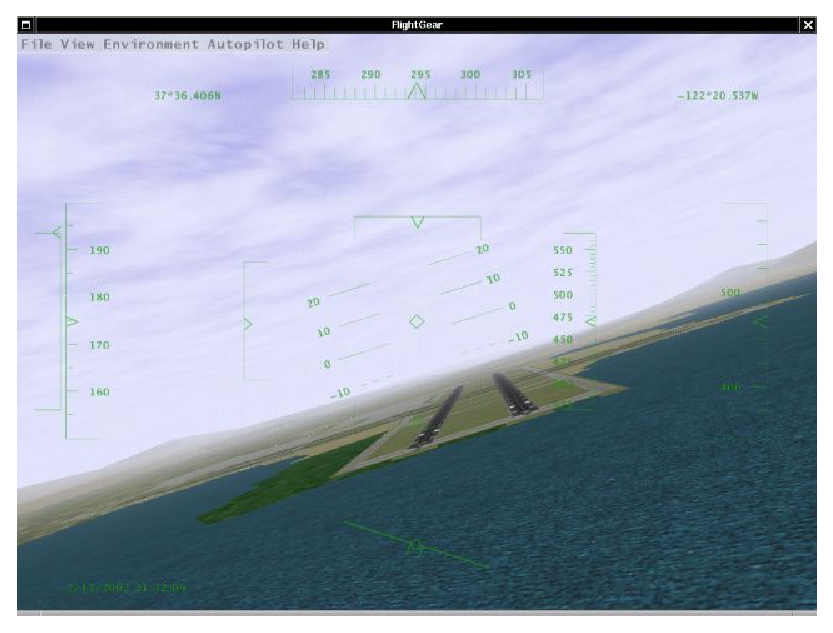
\includegraphics[clip,width=12.5cm]{KSFOapp}
}}

\smallskip
 \noindent
Fig.\,1: \textit{\FlightGear{} under UNIX: Bad approach to San Francisco International - by one of the authors of this manual\ldots}

%%%%%%%%%%%%%%%%%%%%%%%%%%%%%%%%%%%%%%%%%%%%%%%%%%%%%%%%%%%%%%%%%%%%%%%%%%%%%%%%%%%%%%%%%%%%%%%
\section{System Requirements}\index{system requirements}
%%%%%%%%%%%%%%%%%%%%%%%%%%%%%%%%%%%%%%%%%%%%%%%%%%%%%%%%%%%%%%%%%%%%%%%%%%%%%%%%%%%%%%%%%%%%%%%
In comparison to other recent flight simulators, the \Index{system requirements} for
\FlightGear{} are not extravagant. A decent PIII/800, or something in that range, should be
sufficient given you have a proper 3-D \Index{graphics card}. Additionally, any
modern \Index{UNIX}-type \Index{workstation} with a 3-D graphics card will handle
\FlightGear{} as well.

One important prerequisite for running \FlightGear{} is a graphics card whose driver supports
\Index{OpenGL}. If you don't know what \Index{OpenGL} is, the overview given at the OpenGL website
\medskip

\web{http://www.opengl.org}
\medskip

\noindent
 says it best: ``Since its introduction in 1992, OpenGL has become the
industry's most widely used and supported 2-D and 3-D graphics application programming
interface (API)...''.

\FlightGear{} does not run (and will never run) on a graphics board which only supports
\Index{Direct3D}. Contrary to OpenGL, Direct3D is a proprietary interface, being restricted to
the Windows operating system.

You may be able to run \FlightGear{} on a computer that features a 3-D video card not
supporting hardware accelerated \Index{OpenGL} -- and even on systems without 3-D
graphics hardware at all. However, the absence of hardware accelerated OpenGL support can bring even the fastest machine to its knees. The typical signal for missing hardware acceleration
are \Index{frame rate}s below 1 frame per second.

Any modern 3-D graphics featuring \Index{OpenGL} support will do. For
\Index{Windows} video card drivers that support OpenGL, visit the home page of your video
card manufacturer. You should note that sometimes OpenGL drivers\index{OpenGL!drivers}
are provided by the manufacturers of the graphics chip instead of by the makers of the
board. If you are going to buy a graphics card for running \FlightGear{}, one based on a
NVIDIA chip (TNT X/Geforce X) might be a good choice.

To install the executable and basic scenery, you will need around 50 MB of free \Index{disk
space}. In case you want/have to compile the program yourself you will need about an additional
500 MB for the source code and for temporary files created during compilation. This does not
include the development environment, which will vary in size depending on the operating system
and environment being used.  Windows users can expect to need approximately 300 MB of additional
disk space for the development environment.  Linux and other UNIX machines should have most of
the development tools already installed, so there is likely to be little additional space
needed on those platforms.

For the \Index{sound effects}, any capable \Index{sound card} should suffice.
Due to its flexible design, \FlightGear{} supports a wide range of \Index{joysticks} and
\Index{yokes} as well as \Index{rudder pedals} under \Index{Linux} and \Index{Windows}. 
\FlightGear{} can also provide interfaces to full-motion flight chairs.

\FlightGear{} is being developed primarily under \Index{Linux}, a free UNIX clone
(together with lots of GNU utilities) developed cooperatively over the Internet in much
the same spirit as \FlightGear{} itself. \FlightGear{} also runs and is partly developed
under several flavors of \Index{Windows}. Building \FlightGear{} is also possible on a Macintosh OSX
and several different UNIX/X11 workstations. Given you have a proper \Index{compiler} installed,
\FlightGear{} can be built under all of these platforms. The primary compiler for all platforms is
the free \Index{GNU C++} compiler (the \Index{Cygnus} \Index{Cygwin} compiler under Win32).

If you want to run \FlightGear{} under Mac OSX we suggest a Power PC G3 300 MHz or better. As a
graphics card we would suggest an ATI Rage 128 based card as a minimum. Joysticks are supported
under Mac OS 9.x only; there is no joystick support under Max OSX at this time.


%%%%%%%%%%%%%%%%%%%%%%%%%%%%%%%%%%%%%%%%%%%%%%%%%%%%%%%%%%%%%%%%%%%%%%%%%%%%%%%%%%%%%%%%%%%%%%%
\section{Choosing A Version}\index{FlightGear!versions}
%%%%%%%%%%%%%%%%%%%%%%%%%%%%%%%%%%%%%%%%%%%%%%%%%%%%%%%%%%%%%%%%%%%%%%%%%%%%%%%%%%%%%%%%%%%%%%%

Concerning the \FlightGear{} source code there exist two branches, a stable branch and a
developmental branch.\index{branch, stable}\index{branch, developmental} Even version numbers
like 0.6, 0.8, and (someday hopefully) 1.0 refer to stable releases, while odd
numbers like 0.7, 0.9, and so on refer to developmental releases. The policy is to only do
bug fixes in the even versions, while new features are generally added to odd-numbered
versions which, after all things have stabilized, will become the next stable release
with a version number calculated by adding 0.1.\label{branches}

To add to the confusion, there usually are several versions of the ``unstable''
branch. First, there is a ``latest official release'' which the pre-compiled binaries are based
on.  It is available from
\medskip

\web{ftp://ftp.flightgear.org/pub/fgfs/Source/FlightGear-X.Y.Z.tar.gz}
\medskip

For developers there exist CVS snapshots\index{CVS snapshots}\index{nightly snapshots} of the
source code, available from
 \medskip

\web{ftp://www.flightgear.org/pub/flightgear/Devel/Snapshots/}.
 \medskip

 \noindent
While theses are quite recent, they may still be sometimes a few days back behind
development. Thus, if you really want to get the very latest and greatest (and, at times,
buggiest) code, you can use a tool called \Index{anonymous cvs}\index{cvs, anonymous}
available from
 \medskip

\web{http://www.cvshome.org/}
 \medskip

 \noindent
to get the recent code. A detailed description of how to set this up for \FlightGear{}
can be found at
 \medskip

\web{http://www.flightgear.org/cvsResources/}.
 \medskip

 \noindent
 Unfortunately, the system implemented above does not really work as it should. As a matter of
 fact, the stable version is usually so much outdated, that it does not at all reflect the state
 of development \FlightGear{} has reached. Given that the recent developmental versions on the
 other hands may contain bugs (\ldots undocumented features), we recommend using the
 ``latest official (unstable) release'' for the average user. This is the latest version named at

 \web{http://www.flightgear.org/News/};
 \medskip

\noindent
 usually this is also the version which the binary distributions\index{distribution!binary}
 available at
 \medskip

\web{http://www.flightgear.org/Downloads/}
 \medskip

 \noindent
 are based on. If not otherwise stated, all procedures in this ``Installation and Getting Started''
 will be based on these packages.

%%%%%%%%%%%%%%%%%%%%%%%%%%%%%%%%%%%%%%%%%%%%%%%%%%%%%%%%%%%%%%%%%%%%%%%%%%%%%%%%%%%%%%%%%%%%%%%
\section{Flight Dynamics Models\label{flightmodels}}\index{flight dynamics model}\index{flight model}
%%%%%%%%%%%%%%%%%%%%%%%%%%%%%%%%%%%%%%%%%%%%%%%%%%%%%%%%%%%%%%%%%%%%%%%%%%%%%%%%%%%%%%%%%%%%%%%
Historically, \FlightGear{} has been based on a flight model it inherited (together
with the Navion airplane) from LaRCsim. As this had several limitations (most important,
many characteristics were hard wired in contrast to using configuration files), there were
several attempts to develop or include alternative \Index{flightmodels}. As a result,
\FlightGear{} supports several different flight models, to be chosen from at runtime.

The most important one is the JSB flight model developed by Jon Berndt. Actually, the JSB
flight model is part of a stand-alone project called \JSBSim, having its home at
 \medskip

\web{http://jsbsim.sourceforge.net/}.
 \medskip

 \noindent
Concerning airplanes, the JSB flight model at present provides support for a
\Index{Cessna 172}, a \Index{Cessna 182}, a \Index{Cessna 310}, and for an experimental plane
called \Index{X15}. Jon and his group are gearing towards a very accurate flight model, and the
JSB model has become \FlightGear{}'s default flight model.

As an interesting alternative, Christian Mayer developed a flight model of a hot air
balloon. Moreover, Curt Olson integrated a special ``UFO'' slew mode, which
helps you to quickly fly from point A to point B.

Recently, Andrew Ross contributed another flight model called \YASim{}\index{YASim} for
\textit{Yet Another Simulator}. At present, it sports another \Index{Cessna 172}, a
\Index{Turbo 310}, a fairly good \Index{DC-3} model, along with a \Index{Boeing 747},
\Index{Harrier}, and \Index{A4}. \YASim{} takes a fundamentally different approach since it's
based on geometry information rather than aerodynamic coefficients. Where \JSBSim{} will be exact for every situation that is known and flight tested, but may have odd and/or unrealistic behavior outside normal flight, \YASim{} will be sensible and consistent in almost every flight situation, but is likely to differ in performance numbers.

As a further alternative, there is the \Index{UIUC flight model}, developed by a 
team at the University of Illinois at Urbana-Champaign.  This work was 
initially geared toward modeling aircraft in icing conditions\index{icing!modelling} together with a smart icing system to better enable pilots to fly safely in an icing 
encounter.  While this research continues, the project has expanded to 
include modeling ``nonlinear'' aerodynamics, which result in more realism 
in extreme attitudes, such as stall and high angle of attack flight.  Two 
good examples that illustrate this capability are the \Index{Airwave Xtreme 150} 
\Index{hang glider} and the 1903 \Index{Wright Flyer}.  For the hang glider, throttle can 
be use to fly to gliding altitude or Ctrl-U can be used to jump up in 
1000-ft increments.  Try your hand at the unstable Wright Flyer and don't 
stall the canard!  Considerable up elevator trim will be required for level 
flight.  In general, the aerodynamics are probably very close to the 
original Wright Flyer as they are partly based on experimental data taken 
on a replica tested recently at the NASA Ames Research Center.  Also 
included are two more models, a \Index{Beech 99} and \Index{Marchetti S-211} jet trainer, 
which are older generation UIUC/FGFS models and based on simpler ``linear'' 
aerodynamics.  More details of the UIUC flight model and a list of aircraft 
soon to be upgraded can be found on their website at
\medskip

\href{http://amber.aae.uiuc.edu/~m-selig/apasim.html}{http://amber.aae.uiuc.edu/\~{}m-selig/apasim.html}
\medskip

\noindent
Note that the 3D models of the UIUC airplanes\index{UIUC airplanes!3D models} can be downloaded from a site maintained by Wolfram Kuss
\medskip

\web{http://home.t-online.de/home/Wolfram.Kuss/}
\medskip

It is even possible to drive FlightGear's scene display using an external
FDM\index{FDM!external} running on a different computer or via named
pipe\index{FDM!pipe} on the local machine -- although this might not be a
setup recommended to people just getting in touch with \FlightGear.


%%%%%%%%%%%%%%%%%%%%%%%%%%%%%%%%%%%%%%%%%%%%%%%%%%%%%%%%%%%%%%%%%%%%%%%%%%%%%%%%%%%%%%%%%%%%%%%
\section{About This Guide}
%%%%%%%%%%%%%%%%%%%%%%%%%%%%%%%%%%%%%%%%%%%%%%%%%%%%%%%%%%%%%%%%%%%%%%%%%%%%%%%%%%%%%%%%%%%%%%%
\markright{\thesection.\hspace*{1mm} ABOUT THIS GUIDE}

There is little, if any, material in this Guide that is presented here exclusively. You
could even say with Montaigne that we ``merely gathered here a big bunch of other men's
flowers, having furnished nothing of my own but the strip to hold them together''. Most
(but fortunately not all) of the information herein can also be obtained from the
\FlightGear{} web site\index{FlightGear Website} located at
\medskip

\web{http://www.flightgear.org/}
\medskip

Please, keep in mind that there are several mirrors of the \FlightGear{} web sites, all
of which are linked to from the \FlightGear{} homepage listed above.
You may prefer to download \FlightGear{} from a mirror closer to you than from the
main site.

This \textit{\FlightGear{} Installation and Getting Started} manual is intended to be a
first step towards a complete \FlightGear{} documentation\index{FlightGear
documentation}. The target
audience is the end-user who is not interested in the internal workings of \Index{OpenGL}
or in building his or her own scenery. It is our hope, that someday there
will be an accompanying \textit{\FlightGear{} Programmer's Guide}\index{FlightGear
Programmer's Guide} (which could be based on some of the documentation found at
 \medskip

\web{http://www.flightgear.org/Docs};
 \medskip

 \noindent
a \textit{\FlightGear{} Scenery Design Guide},\index{FlightGear Scenery Design Guide}
describing the Scenery tools now packaged as \TerraGear{}; and a \textit{\FlightGear{}
Flight School}\index{FlightGear Flight School} package.
 \medskip

As a supplement, we recommend reading the \FlightGear{} FAQ to be found at

\web{http://www.flightgear.org/Docs/FlightGear-FAQ.html}

which has a lot of supplementary information that may not be included in this manual.

\textbf{We kindly ask you to help us refine this document by submitting corrections,
improvements, and suggestions. All users are invited to contribute descriptions of alternative
setups (graphics cards, operating systems etc.). We will be more than happy to include
those into future versions of this \textit{Installation and Getting Started} (of course
not without giving credit to the authors).}

While we intend to continuously update this document, we may not be able to produce a
new version for every single release of {\FlightGear{}}.  To do so would require more
manpower that we have now, so please feel free to jump in and help out.  We hope to
produce documentation that measures up to the quality of \FlightGear{} itself.


%% Revision 0.00  1998/09/08  michael
%% Initial revision for version 0.53.
%% Revision 0.01  1998/09/20  michael
%% several extensions and corrections
%% revision 0.10  1998/10/01  michael
%% final proofreading for release
%% revision 0.11  1998/11/01  michael
%% minor corrections on platforms, satellite data, OpenGL
%% added Navion pic
%% revision 0.12  1999/03/07  michael
%% update on recent development
%% revision 0.20  1999/06/04  michael
%% updates on recent development, corrections of links
%% revision 0.3 2000/04/20 michael
%% Rewritten for version 0.7.2, many changes, added development since summer 1999,
%% development vs. stable version, split into SimGear/FlightGear/TerraGear
%% Proofread by Jon Berndt
%% revision 0.4 2001/05/12 michael
%% update on development during the last year, corrections on requirements,
%% new sections on different versions and on flight models
%% revision 0.41 2001/07/01 martin & michael
%% comment on external FDM
%% hint to FAQ
%% extended remarks on property manager
%% revision 0.5 2002/01/01 michael
%% several minor updates, corrected links
%% Hint on YASim by Martin
%% Picture KSFOapp added by Martin
%% System requirements contributed from Darrell
%% revision 0.6 2002/02/23 cameron
%% Many, many corrections
%% Rewrote several parts
%% Changed section titles
%% revision 0.6 2002/09/07 michael
%% Added contribution by M Selig on UIUC models
%% 3 minor typo/grammar edits by Dave Perry 
%% (P.12 replaced double apostrophe, p.14 <<<to to  >>> to, <<<users is >>>users are

%%
%% getstart.tex -- Flight Gear documentation: The FlightGear Manual
%% Chapter file
%%
%% Written by Michael Basler, started September 1998.
%%
%% Copyright (C) 2002 Michael Basler
%%
%%
%% This program is free software; you can redistribute it and/or
%% modify it under the terms of the GNU General Public License as
%% published by the Free Software Foundation; either version 2 of the
%% License, or (at your option) any later version.
%%
%% This program is distributed in the hope that it will be useful, but
%% WITHOUT ANY WARRANTY; without even the implied warranty of
%% MERCHANTABILITY or FITNESS FOR A PARTICULAR PURPOSE.  See the GNU
%% General Public License for more details.
%%
%% You should have received a copy of the GNU General Public License
%% along with this program; if not, write to the Free Software
%% Foundation, Inc., 675 Mass Ave, Cambridge, MA 02139, USA.
%%
%% $Id: prefligh.tex,v 0.6 2002/09/09 michael
%% (Log is kept at end of this file)

%%%%%%%%%%%%%%%%%%%%%%%%%%%%%%%%%%%%%%%%%%%%%%%%%%%%%%%%%%%%%%%%%%%%%%%%%%%%%%%%%%%%%%%%%%%%%%%
\ifchinese
\chapter{{\\}飞行前:安装 \FlightGear{}}
\fi
\IfLanguageName{french}{
\chapter{Pr\'{e}vol : installer \FlightGear{}}
}{}
\IfLanguageName{italian}{
\chapter{Prima di volare: installazione di \FlightGear{}}
}{}
\label{prefligh}
%%%%%%%%%%%%%%%%%%%%%%%%%%%%%%%%%%%%%%%%%%%%%%%%%%%%%%%%%%%%%%%%%%%%%%%%%%%%%%%%%%%%%%%%%%%%%%%

\ifchinese
若要运行 \FlightGear{} 你需要安装二进制程序。之后如果你愿意,还可以安装额外的地景和航空器。

最新发布的预先编译的二进制程序,支持如下平台

\begin{itemize}
\item Windows - 任何版本
\item Mac OS X
\item Linux
\end{itemize}

要下载请前往

\medskip
\web{http://www.flightgear.org/download/main-program/}
\medskip
\fi
%\IfLanguageName{english}{
%To run \FlightGear{} you need to install the binaries. Once you've done this you may install additional scenery and aircraft if you wish.
%
%Pre-compiled binaries for the latest release are available for
%
%\begin{itemize}
%\item Windows - any flavor,
%\item Mac OS X,
%\item Linux.
%\end{itemize}
%
%To download them go to
%
%\medskip
%\web{http://www.flightgear.org/download/main-program/}
%\medskip
%
%and follow the instructions provided on the page.
%}{}

\IfLanguageName{french}{
Pour faire fonctionner \FlightGear{}, vous devez en installer les binaires. Une fois que vous aurez fait ceci vous pourrez, si vous le souhaitez, installer les paysages et avions additionnels.

Les binaires pr\'{e}-compil\'{e}s de la derni\`{e}re version sont disponibles pour :

\begin{itemize}
\item Windows - toutes versions,
\item Mac OS X,
\item Linux.
\end{itemize}

Pour les t\'{e}l\'{e}charger, rendez-vous sur la page :

\medskip
\web{http://www.flightgear.org/download/main-program/}
\medskip

et suivez les instructions qui y sont pr\'{e}sentes.
}{}

\IfLanguageName{italian}{
Per eseguire  \FlightGear{}\`{e} necessario installare i file binari. Una
volta fatto questo \`{e} possibile installare scenari e velivoli aggiuntivi, se lo si desidera.
File binari pre-compilati per l'ultima versione sono disponibili per:

\begin{itemize}
\item Microsoft Windows - qualsiasi versione
\item Mac OS X
\item Linux
\end{itemize}

Per scaricarli, andare sul sito
\web{http://www.flightgear.org/download/main-program/}
e seguire le istruzioni fornite nella pagina.
}{}


%%%%%%%%%%%%%%%%%%%%%%%%%%%%%%%%%%%%%%%%%%%%%%%%%%%%%%%%%%%%%%%%%%%%%%%%%%%%%%%%%%%%%%%%%%%%%%%
\ifchinese
\section{安装地景}\index{scenery 地景!额外的}\index{额外地景}\index{scenery 地景}
\fi
%\IfLanguageName{english}{
%\section{Installing scenery}\index{scenery!additional}\index{additional scenery}\index{scenery}
%}{}
\IfLanguageName{french}{
\section{Installer des sc\`{e}nes}\index{scenery!additional}\index{additional scenery}\index{sc\`{e}enes}
}{}
\IfLanguageName{italian}{
\section{Installare scenari}\index{scenery!additional}\index{additional scenery}\index{scenari}
}{}
%%%%%%%%%%%%%%%%%%%%%%%%%%%%%%%%%%%%%%%%%%%%%%%%%%%%%%%%%%%%%%%%%%%%%%%%%%%%%%%%%%%%%%%%%%%%%%%

\ifchinese
\FlightGear{} 的详细地景可以覆盖整个世界,从世界之巅的喜马拉雅山脉到堪萨斯乡村,都可以任君自由飞行。\FlightGear{}  的基础包包括了檀香山及周边岛屿在内的一小片区域,所以要想飞到其他地方,就需要下载额外地景。

每一块地景都被打包成了一个压缩文件,或者一个 tarball,每经纬度10度为一块。每一个 tarball 以 10 x 10 经纬度块来命名,比如 w130n50.tgz。

要下载你想要飞行的区域,可以在启动器里启用 TerraSync 这样就会启用自动下载。你

也可以在模拟器之外,使用下面这个可以点选的地图里下载或使用 TerraMaster 工具:
\fi
%\IfLanguageName{english}{
%Detailed \FlightGear{} scenery is available for the entire world, allowing
%you to fly everywhere from the Himalaya mountains to rural Kansas.
%The \FlightGear{} base package contains scenery for a small area around San
%Francisco, so to fly elsewhere you will need to download additional scenery.
%
%Each piece of scenery is packaged into a compressed archive, or tarball, in
%a 10 degree by 10 degree chunk. Each tarball is named after the 10x10 degree
%chunk it represents, for example w130n50.tgz.
%
%You can download scenery from a clickable map here:
%}{}

\IfLanguageName{french}{
Des sc\`{e}nes d\'{e}taill\'{e}es de \FlightGear{} sont disponibles pour le monde entier,
vous permettant de voler n'importe o\`{u}, des sommets de l'Himalaya \`{a} la campagne du Kansas.
Le paquetage de base de \FlightGear{} comprend les sc\`{e}nes d'une petite zone autour de San
Francisco, donc pour aller voler dans d'autres parties du monde vous aurez besoin de t\'{e}l\'{e}charger des
sc\`{e}nes additionnelles.

Chaque portion de sc\`{e}ne est regroup\'{e}e dans une archive compress\'{e}e (appel\'{e}e \textit{tarball}, en anglais),
qui correspond \`{a} une tuile de 10 degr\'{e}s par 10 degr\'{e}s. Chaque archive est nomm\'{e}e en fonction de la tuile
de 10x10 degr\'{e}s qu'elle repr\'{e}sente, par exemple w130n50.tgz.

Vous pouvez t\'{e}l\'{e}charger les sc\`{e}nes \`{a} partir d'une carte cliquable ici :
}{}

\IfLanguageName{italian}{
ono disponibili scenari dettagliati raffiguranti tutto il mondo, che consentono di volare
ovunque, dalle montagne dell'Himalaya al rurale Kansas. Il pacchetto base di \FlightGear{}
contiene scenari per una piccola area intorno a San Francisco, per volare altrove \`{e}
necessario scaricare uno scenario aggiuntivo.
Ogni pezzo di scenario 10x10 gradi (latitudine e longitudine) viene compresso in un
archivio (solitamente di formato, .rar, .tar o .tgz). Ogni archivio \`{e} chiamato con
le coordinate che rappresenta, per esempio ''w130n50.tgz''
\'{E} possibile scaricare gli scenari ufficiali da un planisfero cliccabile qua:
}{}

\medskip

\web{http://wiki.flightgear.org/TerraSync}

\web{http://www.flightgear.org/download/scenery/}

\web{http://wiki.flightgear.org/TerraMaster}
\medskip

\ifchinese
另外,你可以通过购买覆盖全世界的完整地景集来支持 \FlightGear{}:
\fi
%\IfLanguageName{english}{
%Alternatively, you can support the \FlightGear{} project by purchasing a complete
%set of scenery for the entire world from here:
%}{}

\IfLanguageName{french}{
Sinon, vous pouvez soutenir le projet \FlightGear{} en achetant un lot complet des sc\`{e}nes du monde entier
sur DVD \`{a} l'adresse :
}{}

\IfLanguageName{italian}{
In alternativa, \`{e} possibile sostenere il progetto \FlightGear{} con l'acquisto del set completo
di scenari per il mondo intero da qui:
}{}

\medskip
\web{http://shopping.flightgear.org/}
\medskip

\ifchinese
你下载了 tarball 到你的电脑上以后,首先需要找到 \FlightGear{} 的 \texttt{Scenery} 安装目录。
\fi
%\IfLanguageName{english}{
%Once you have downloaded the tarball onto your computer, you need to find the
%\texttt{Scenery} directory of your \FlightGear{} installation.
%}{}

\IfLanguageName{french}{
Une fois le fichier compress\'{e} t\'{e}l\'{e}charg\'{e} sur votre ordinateur, il vous faut localiser
le r\'{e}pertoire \texttt{Scenery} de votre installation \FlightGear{}.
}{}

\IfLanguageName{italian}{
Dopo aver scaricato gli archivi sul computer, \`{e} necessario trovare la directory di \FlightGear{}
contenente gli scenari
}{}

\begin{itemize}
\ifchinese
\item 对 Windows 而言,可能在这样的文件夹下:
\fi
%\IfLanguageName{english}{
%\item For Windows, this directory is likely to be
%}{}
\IfLanguageName{french}{
\item Pour Windows, ce r\'{e}pertoire devrait \^{e}tre :
}{}
\IfLanguageName{italian}{
\item In Windows questa cartella \`{e} probabile che sia:
}{}

\texttt{c:$\backslash$Program Files$\backslash$FlightGear$\backslash$data$\backslash$Scenery}.

\ifchinese
\item 对各种 UNIX 系统,通常是:
\fi
%\IfLanguageName{english}{
%\item For Unices, it is usually
%}{}

\IfLanguageName{french}{
\item Pour les machines fonctionnant sous la famille Unix, il s'agit g\'{e}n\'{e}ralement du r\'{e}pertoire :
}{}

\IfLanguageName{italian}{
\item Per i sistemi UNIX, di solito \`{e}:
}{}

\texttt{/usr/local/share/FlightGear/data/Scenery}.

\ifchinese
\item 对 Mac OS X,可能是这种:
\fi
%\IfLanguageName{english}{
%\item For Mac OS X, it is usually either
%}{}

\IfLanguageName{french}{
\item Pour Mac OS X, il s'agit g\'{e}n\'{e}ralement de:
}{}

\IfLanguageName{italian}{
\item Per Mac OS X, \`{e} solitamente:
}{}

\texttt{/Applications/FlightGear.app/Contents/Resources/data/Scenery}.

\end{itemize}

\ifchiense
要安装地景,首先解压缩 tarball 到 \texttt{Scenery} 目录。大多数操作系统提供了解压缩 tarball 的工具。如果你不能解压缩 tarball,可以安装相应的程序比如 7-zip(\web{http://www.7-zip.org/})。

注意不要解压缩 tarball 包里像 958402.gz 这样以数字命名的地景文件——这会由 \FlightGear{} 在飞行时自动解压。

解压了 tarball 以后,\texttt{Terrain} 和 \texttt{Objects} 目录会包含额外的子目录,里面有新加的地景。

要使用新的地景,只需要选择地景所在区域的机场。如果你在使用 \FlightGear{} 启动器(FlightGear Launcher),选择机场前请先按刷新按钮。
\fi
%\IfLanguageName{english}{
%To install the scenery, uncompress the tarball into the \texttt{Scenery}
%directory. Most operating system provide tools to uncompress tarballs. If you cannot
%uncompress the tarball, install an extractor program such as 7-zip
%(\web{http://www.7-zip.org/}).
%
%Note that you should not decompress the numbered scenery files inside the tarball like
%958402.gz - this will be done by \FlightGear{} on the fly.
%
%Once you have uncompressed the tarball, the \texttt{Terrain} and \texttt{Objects} directories
%will contain additional sub-directories with your new scenery inside.
%
%To use the new scenery, simply select a starting airport within the new scenery.
%If you are using the \FlightGear{} Launcher, you will need to press the Refresh
%button before you select your airport.
%}{}

\IfLanguageName{french}{
Pour installer les sc\`{e}nes, d\'{e}compressez le fichier compress\'{e} dans le r\'{e}pertoire \texttt{Scenery}.
La plupart des syst\`{e}mes d'exploitation propose des outils pour d\'{e}compresser des fichiers type \textit{tarball}.
Si vous ne parvenez par \`{a} le d\'{e}compresser, installez un programme d'extraction comme 7-zip
(\web{http://www.7-zip.org/}).

Notez que vous ne devez pas d\'{e}compresser les fichiers de sc\`{e}nes num\'{e}rot\'{e}s pr\'{e}sents au sein du fichier
\textit{tarball}, comme par exemple 958402.gz - cette action sera r\'{e}alis\'{e}e \`{a} la vol\'{e}e par \FlightGear{}.

Une fois que ce fichier est d\'{e}compress\'{e}, les r\'{e}pertoires \texttt{Terrain} et \texttt{Objects} contiendront de
nouveaux sous-r\'{e}pertoires o\`{u} se situent vos nouvelles sc\`{e}nes.

Pour utiliser ces nouvelles sc\`{e}nes, rendez-vous simplement \`{a} l'a\'{e}roport de d\'{e}marrage de votre choix situ\'{e} au sein
de la nouvelle sc\`{e}ne. Si vous utilisez l'assistant de d\'{e}marrage de \FlightGear{}, vous devrez appuyer sur le
bouton Rafra\^{i}chir avant de choisir votre a\'{e}roport.
}{}

\IfLanguageName{italian}{
Per installare gli scenari, decomprimere l'archivio nella directory Scenery.
La maggior parte dei sistemi operativi fornisce gli strumenti per decomprimere gli archivi.
Se ci\`{o} non fosse, installare un programma estrattore come 7-zip (\web{http://www.7-zip.org/}).
Si noti che non \`{e} necessario decomprimere i file numerati all'interno dell'archivio
come \texttt{958402.tgz} - questo sar\`{a} fatto da FlightGear durante il volo.
Dopo aver decompresso l'archivio, le directory \texttt{Terrain} e \texttt{Objects} conterranno
ulteriori sotto-cartelle con il nuovo scenario all'interno.
Per utilizzare il nuovo scenario, \`{e} sufficiente selezionare nella schermata di
avvio del simulatore un aeroporto di partenza contenuto nello scenario.
Se si utilizza il Launcher di FlightGear, sar\`{a} necessario premere il
pulsante \texttt{Aggiorna} prima di selezionare l'aeroporto.
}{}

\subsection{MS Windows Vista/7}
\ifchinese
如果你使用 Windows Vista 或 Windows 7,会发现 Windows 把安装下载的地景(和航空器)放到你的 Virtual Store 目录下:
\fi
%\IfLanguageName{english}{
%If you are using Windows Vista or Windows 7, you may find that Windows installs downloaded scenery
%(and aircraft) to your Virtual Store:
%}{}
\IfLanguageName{french}{
Si vous utilisez Windows Vista ou Windows 7, vous pourriez \^{e}tre confontr\'{e} au fait que Windows installe
les sc\`{e}nes (et a\'{e}ronefs) t\'{e}l\'{e}charg\'{e}s dans votre Virtual Store :
}{}
\IfLanguageName{french}{
Se si utilizza Windows Vista o Windows 7, \`{e} possibile che Windows posizioni gli scenari scaricati
(e gli aeromobili) al Virtual Store:
}{}

\noindent

\ifchinese
  \noindent { \footnotesize{\texttt{c:\char`\\Users\char`\\(Your Name)\char`\\AppData\char`\\Local\char`\\}

  \hspace*{3em}\texttt{VirtualStore\char`\\Program Files\char`\\FlightGear\char`\\Scenery}}}
\fi
%\IfLanguageName{english}{
%{ \footnotesize{\texttt{c:$\backslash$Users$\backslash$(Your
%Name)$\backslash$AppData$\backslash$Local$\backslash$VirtualStore$\backslash$Program
%Files$\backslash$FlightGear$\backslash$Scenery}}}
%}{}
\IfLanguageName{french}{
{ \footnotesize{\texttt{c:$\backslash$Users$\backslash$(Votre Nom)$\backslash$AppData$\backslash$Local$\backslash$VirtualStore$\backslash$Program Files$\backslash$FlightGear$\backslash$Scenery}}}
}{}
\IfLanguageName{italian}{
{ \footnotesize{\texttt{c:$\backslash$Users$\backslash$(tuo nome)$\backslash$AppData$\backslash$Local$\backslash$VirtualStore$\backslash$Program Files$\backslash$FlightGear$\backslash$Scenery}}}
}{}

\ifchinese
如果是这样的话,你需要把 \texttt{Terrain} 和 \texttt{Objects} 目录手动拷贝到如上面所说 \FlightGear{} 的实际 \texttt{Scenery} 目录。
\fi
%\IfLanguageName{english}{
%If it does this, you need to copy the \texttt{Terrain} and \texttt{Objects}
%directories manually to your real \FlightGear{} \texttt{Scenery} directory
%as described above.
%}{}

\IfLanguageName{french}{
S'il le fait, vous devrez copier manuellement les r\'{e}pertoires \texttt{Terrain} et \texttt{Objects}
vers votre v\'{e}ritable r\'{e}pertoire \texttt{Scenery} de \FlightGear{}, comme cela a \'{e}t\'{e} d\'{e}crit ci-dessus.
}{}

\IfLanguageName{italian}{
Se dovesse succedere questo, \`{e} necessario copiare manualmente i file nella directory reale degli scenari
di FlightGear come descritto sopra.
}{}

\subsection{Mac OS X \label{sceneryOnMac}}
\ifchinese
你可以使用图形化(GUI)启动器安装下载的地景数据和航空器。在 \textit{Advanced Features >> Others} 选项卡上找到 \textit{Install Add-On data} 按钮,将会打开一个文件浏览窗口。选择一个或多个地景数据文件,将会安装这些地景到 \\ \texttt{/Applications/FlightGear.app/Contents/Resources/data/Scenery}\\可以接受的地景文件类型可以是 zip、tar.gz、tgz、tar 和已经解压缩的文件夹。如果使用图形化启动器安装时因为某些原因失败的话,你可以用替代方法安装数据。打开数据文件夹,按“其他”选项卡上“Open data folder”会弹出一个 Finder 窗口。拖拽一个地景文件夹到 data 文件夹下的 data/Scenery 文件夹(或一个航空器文件夹到 data/Aircraft 文件夹),就可以了。
\fi
%\IfLanguageName{english}{
%You may install the downloaded scenery data and aircraft using the GUI launcher. Pressing \textit{Install Add-On data}
%on the \textit{Advanced Features >> Others} tab opens up the file browser window. Selecting one or more scenery data
%files will install the scenery data into \texttt{/Applications/FlightGear.app/Contents/Resources/data/Scenery}. Acceptable
%formats for the scenery data are one of zip, tar.gz, tgz, tar, and extracted folder. If the installation via the
%GUI launcher failure for some reason, you still have an alternative way to install the data. Opening the data folder
%by pressing ``Open data folder'' on the Others tab will pop up an Finder window for the data folder. Dragging an
%aircraft folder to data/Aircraft folder (or a scenery folder to data/Scenery folder) under the data folder will get the job done.
%}{}
\IfLanguageName{french}{
Vous pouvez installer les donn\'{e}es des sc\`{e}nes et des avions t\'{e}l\'{e}charg\'{e}s en utilisant l'interface
de lancement (GUI launcher). Appuyez sur \textit{Installez des donn\'{e}es additionnelles} dans l'onglet
\textit{Fonctionnalit\'{e}s avanc\'{e}es >> Autres}, ceci ouvrira la fen\^{e}tre d'exploration des fichiers.
En choisissant un ou plusieurs fichiers de sc\`{e}nes, ceci installera les donn\'{e}es de sc\`{e}nes dans
\texttt{/Applications/FlightGear.app/Contents/Resources/data/Scenery}. Les formats acceptables pour les donn\'{e}es de
sc\`{e}nes sont zip, tar.gz, tgz, tar, et dossier extrait. Si l'installation via le GUI launcher ne fonctionne pas,
pour quelque raison que ce soit, vous avez toujours une possibilit\'{e} alternative d'installer les donn\'{e}es.
Ouvrez le fichier de donn\'{e}es en appuyant sur ``Ouvrir le fichier de donn\'{e}es'' dans l'onglet Autres. Vous
ouvrirez ainsi une fen\^{e}tre Rechercher pour le r\'{e}pertoire des donn\'{e}es. Glisser le r\'{e}pertoire d'un
avion vers le r\'{e}pertoire data/Aircraft (ou un r\'{e}pertoire de sc\`{e}nes vers un r\'{e}pertoire data/Scenery)
sous le r\'{e}pertoire donn\'{e}es permettra d'aboutir au m\^{e}me r\'{e}sultat.
}{}

\IfLanguageName{italian}{
\`{e} possibile installare gli scenari/aeromobili scaricati usando l'interfaccia grafica del Launcher.
Premendo ''Installa Add-On'' nella scheda ''funzioni avanzate'' si dovrebbe aprire una finestra dove
\`{e} possibile selezionare dei file. Selezionando uno o pi\`{u} scenari, questi verranno installati automaticamente in:

\texttt{/Applications/FlightGear.app/Contents/Resources/data/Scenery}

I formati accettabili per gli scenari sono: ''.zip'', ''.rar'', ''.tgz'', ''.tar'', e cartelle gi\`{a} estratte.
Se l'installazione tramite il Launcher dovesse fallire per qualche motivo, \`{e} possibile installarli manualmente.
Per far ci\`{o}, bisogna aprire la cartella dati di FlightGear, premendo "Apri cartella dati" nella scheda ''Altro''
del simulatore. Una volta aperta la cartella, \`{e} possibile copiare i paesaggi/aerei al suo interno.

}{}

\subsection{FG\_SCENERY}\index{FG\_SCENERY}
\ifchinese
如果你想将下载的地景放到与安装位置不同的地方,可以设置 \texttt{FG\_SCENERY} 环境变量。

\FlightGear{} 会到此去寻找地景文件,可以在此按顺序列出要搜索的目录。在 UNIX (包括 Mac OS X)下用“:”分隔,在 Windows 下则用“;”。

例如,Linux 下的 \texttt{FG\_SCENERY} 环境变量可以设置成
\fi
%\IfLanguageName{english}{
%If you would prefer to keep your downloaded scenery separate from the core
%installation, you can do so by setting your \texttt{FG\_SCENERY} environment
%variable.
%
%This is where \FlightGear{} looks for Scenery files. It consists of a list
%of directories that will be searched in order. The directories are separated
%by ``:'' on Unix (including Mac OS X) and ``;'' on Windows.
%
%For example, on Linux a \texttt{FG\_SCENERY} environment variable set to
%}{}

\IfLanguageName{french}{
Si vous pr\'{e}f\'{e}rez conserver vos sc\`{e}nes t\'{e}l\'{e}charg\'{e}es s\'{e}par\'{e}es de
l'installation de base, vous pouvez le faire en pr\'{e}cisant votre variable d'environnement \texttt{FG\_SCENERY}.

Il s'agit de l'emplacement auquel \FlightGear{} recherche des fichiers de sc\`{e}nes. Il contient une liste de
r\'{e}pertoires qui seront analys\'{e}s dans l'ordre. Les r\'{e}pertoires sont s\'{e}par\'{e}s par des ``:'' sous Unix
(dont Mac OS X) et par des ``;'' sous Windows.

Par exemple, sous Linux, une variable d'environnement \texttt{FG\_SCENERY} param\'{e}tr\'{e}e \`{a} :
}{}

\IfLanguageName{italian}{
Se si preferisce mantenere gli scenari scaricati separati dall'installazione di base, \`{e} possibile
farlo impostando la variabile d'ambiente \texttt{FG\_SCENERY}.

Questa variabile contiene i posti dove FlightGear cerca i file degli scenari. Essa consiste di un lista
di directory che saranno esaminate in ordine. Le directory sono separate da '':'' su Unix (incluso Mac OS X)
e da '';'' su Windows.

Ad esempio, su Linux la variabile \texttt{FG\_SCENERY} impostata cos\`{i}:
}{}

\noindent
\texttt{/home/jsmith/WorldScenery:/usr/local/share/Flightgear/data/Scenery}

\noindent
\ifchinese
首先会搜索这里的地景文件\texttt{/home/jsmith/WorldScenery}\\之后则会去
\fi
%\IfLanguageName{english}{
%searches for scenery in \texttt{/home/jsmith/WorldScenery} first, followed by
%}{}
\IfLanguageName{french}{
pr\'{e}cisera \`{a} \FlightGear{} de rechercher des sc\`{e}nes en priorit\'{e} dans le r\'{e}pertoire \texttt{/home/jsmith/WorldScenery}, suivi de :
}{}

\IfLanguageName{italian}{
cercher\`{a} gli scenari prima in:

\texttt{/home/jsmith/WorldScenery}

E poi in:
}{}
\noindent
\texttt{/usr/local/share/Flightgear/data/Scenery}.

\medskip
\ifchinese
在 Windows 下 \texttt{FG\_SCENERY} 环境变量设置成
\fi
%\IfLanguageName{english}{
%On Windows, a \texttt{FG\_SCENERY} environment variable set to
%}{}

\IfLanguageName{french}{
Sous Windows, une variable d'environnement \texttt{FG\_SCENERY} param\'{e}tr\'{e}e \`{a} :
}{}

\IfLanguageName{french}{
In Windows, una variabile di ambiente FG_SCENERY impostata cos\`{i}:
}{}

\texttt{c:\char`\\Program Files\char`\\FlightGear\char`\\data\char`\\Scenery;c:\char`\\data\char`\\WorldScenery}

\noindent
\ifchinese
首先去
\fi
%\IfLanguageName{english}{
%searches for scenery in
%}{}
\IfLanguageName{french}{
cherchera d'abord pour des sc\`{e}nes dans le r\'{e}pertoire :
}{}
\IfLanguageName{italian}{
Cercher\`{a} gli scenari prima in:
}{}
\texttt{c:\char`\\Program Files\char`\\FlightGear\char`\\data\char`\\Scenery}
\medskip
\ifchinese
搜索地景文件,之后
\fi
%\IfLanguageName{english}{
%first, followed by
%}{}
\IfLanguageName{french}{
suivi de :
}{}
\IfLanguageName{italian}{
E poi in :
}{}
\texttt{c:\char`\\data\char`\\WorldScenery}\\
\medskip

\ifchinese
在不同的平台设置环境变量的方法已经超出了本文的范畴,在此不多赘述。
\fi
%\IfLanguageName{english}{
%Setting up environment variables on different platforms is beyond the scope of this document.
%}{}
\IfLanguageName{french}{
Le param\'{e}trage de variables d'environnement sur diff\'{e}rentes plate-formes d\'{e}passe le cadre de ce document.
}{}
\IfLanguageName{italian}{
Come impostare le variabili di ambiente sule diverse piattaforme va oltre lo scopo di questo manuale.
}{}

\ifchinese
\subsection{飞行时获取地景}
\fi
%\IfLanguageName{english}{
%\subsection{Fetch Scenery as you fly}
%}{}
\IfLanguageName{french}{
\subsection{T\'{e}l\'{e}chargez automatiquement des sc\`{e}nes en plein vol}
}{}
\IfLanguageName{italian}{
\subsection{Scaricare scenari mentre si vola}
}{}

\ifchinese
如果你能保证网络的连续性,\FlightGear{} 支持在飞行时获取地景。首先为 \TerraSync{} 创建一个空的“工作”目录,并给予用户可写的权限,并将 \FlightGear{} 地景的 \texttt{FG\_SCENERY} 变量指向相应的路径(如上文所述)。请\textbf{不要}把 \TerraSync{} 下载的地景放到预先安装的地景目录

在 \FlightGear{} 里,到 Environment(环境)菜单下选择 Scenery Download(地景下载)选项。然后选择上面创建的目录并选择 Enable Automatic Scenery(自动地景下载)。

\TerraSync{} 最主要的一个好处是总能从 FlightGear World Scenery 项目下载到最新且最强大的地景文件,因此允许你在 World Scenery 发布之外(通常与 \FlightGear{} 的发布保持同步)进行地景的增量更新。
\fi
%\IfLanguageName{english}{
%\FlightGear{} is able to fetch the Scenery as you fly, if you have a permanent
%Internet connection at your disposal. Create an empty `working'
%directory for \TerraSync{}, writable to the user and point
%\FlightGear{} at this directory using the \texttt{FG\_SCENERY} variable
%(as explained above). Do \textbf{not} let \TerraSync{} download Scenery
%into your pre-installed Scenery directory.
%
%Within \FlightGear{} itself, select the Scenery Download option under the
%Environment menu. Then simply select the directory you created above and
%enable automatic scenery download.
%
%One major benefit of \TerraSync{} is that it always fetches the latest and
%greatest Scenery from the FlightGear World (Custom) Scenery Project and
%therefore allows you to pick up incremental updates independant of the
%comprehensive World Scenery releases, which are generally synchronized
%with \FlightGear{} releases.
%}{}

\IfLanguageName{french}{
\FlightGear{} est capable de t\'{e}l\'{e}charger automatiquement les sc\`{e}nes pendant que
vous volez, si vous avez \`{a} votre disposition une connexion Internet permanente. Cr\'{e}ez un
r\'{e}pertoire de travail `fonctionnel' pour \TerraSync{}, accessible en \'{e}criture pour l'utilisateur
et faites pointer \FlightGear{} vers ce r\'{e}pertoire en utilisant la variable \texttt{FG\_SCENERY}
(comme expliqu\'{e} ci-dessus). Ne laissez \textbf{pas} \TerraSync{} t\'{e}l\'{e}charger des sc\`{e}nes
dans le r\'{e}pertoire Scenery cr\'{e}\'{e} lors de l'installation.

Le probl\`{e}me de la poule et de l'\oe{}uf est pr\'{e}sent lorsque vous d\'{e}marrez pour la premi\`{e}re fois dans
une nouvelle zone. \FlightGear{} s'attend \`{a} trouver les sc\`{e}nes pour cette zone, mais il est possible qu'il ne
les ait pas encore r\'{e}cup\'{e}r\'{e}es. Aussi, d\`{e}s que \TerraSync{} a charg\'{e} la nouvelle tuile (ce que
vous pouvez v\'{e}rifier \`{a} partir de la section Statut de la fen\^{e}tre T\'{e}l\'{e}chargement de sc\`{e}nes),
cliquez sur le bouton Rafra\^ichissement manuel pour recharger les sc\`{e}nes. Si vous rencontrez toujours des
difficult\'{e}s, red\'{e}marrez \FlightGear{}.

Un des b\'{e}n\'{e}fices majeurs de \TerraSync{} est qu'il r\'{e}cup\`{e}re toujours la derni\`{e}re et meilleure
version des sc\`{e}nes \`{a} partir du \textit{\FlightGear{} World (Custom) Scenery Project} et vous permet
ainsi d'obtenir les mises \`{a} jour incr\'{e}mentales ind\'{e}pendamment des versions compl\`{e}tes des sc\`{e}nes
mondiales, qui sont g\'{e}n\'{e}ralement synchronis\'{e}es avec les versions de \FlightGear{}.
}{}

\IfLanguageName{italian}{
FlightGear \`{e} in grado di installare gli scenari mentre si vola, se si dispone di una buona connessione a Internet.
Creare una directory ''working'' vuota e scrivibile per \TerraSync{}, e impostarla affinch\'{e} FlightGear vi cerchi gli
scenari utilizzando la variabile \texttt{FG\_SCENERY} (come spiegato sopra). Non lasciate che \TerraSync{} scarichi gli scenari
nella directory ''Scenery'' pre-installata.
All'interno di FlightGear stesso, selezionare l'opzione ''Download Scenari'' nel men\`{u} ''Ambiente''. Poi basta
selezionare la directory creata sopra e abilitare il download automatico degli scenari.

Uno dei principali vantaggi di \TerraSync{} \`{e} che si ottiene sempre l'ultima versione dello scenario dal database
mondiale di FlightGear.
}{}

\ifchinese
\subsection{独立运行 \TerraSync{}}
\fi
%\IfLanguageName{english}{
%\subsubsection{Running \TerraSync{} as a separate tool}
%}{}
\IfLanguageName{french}{
\subsubsection{Utiliser \TerraSync{} comme un outil s\'{e}par\'{e}}
}{}
\IfLanguageName{italian}{
\subsubsection{Eseguire \TerraSync{} come uno strumento separato}
}{}

\ifchinese
可以将 \TerraSync{} 作为一个外部工具来运行。

在 Mac OS X 或 Windows,只需要在图形化启动器上选择“Download scenery on the fly”,这样就会以一个独立的进程启动 \TerraSync{} 自动下载你飞机周围的地景,因此你根本不用指定 FG\_SCENERY 的地图。

另外你可以直接运行 terrasync 程序。它会告诉 \FlightGear{} 使用“Atlas”协议,因此可以这样调用 \FlightGear{}:
\fi
%\IfLanguageName{english}{
%It is also possible to run \TerraSync{} as an external tool.
%
%On Mac OS X or Windows, just checking ``Download scenery on the fly'' on
%the GUI launcher launches \TerraSync{} as a separate process automatically
%for downloading the Scenery around your aircraft, so you don't have to
%specify the atlas option or FG\_SCENERY at all.
%
%Alternatively you can run the terrasync program directly. It talks to
%\FlightGear{} using the `Atlas' protocol, so call \FlightGear{} with the:
%}{}

\IfLanguageName{french}{
Il est \'{e}galement possible d'utiliser \TerraSync{} comme un outil externe.

Sur Mac OS X ou Windows, le simple fait de cocher ``T\'{e}l\'{e}charger les sc\`{e}nes \`{a} la vol\'{e}e''
dans l'interface graphique de lancement permet d'ex\'{e}ctuer \TerraSync{} de mani\`{e}re automatique dans un
processus s\'{e}par\'{e} pour t\'{e}l\'{e}charger les sc\`{e}nes autour de votre avion, de telle sorte que
vous n'avez pas besoin de sp\'{e}cifier du tout ni l'option atlas, ni FG\_SCENERY.

Sinon, vous pouvez lancer le programme terrasync directement. Il communique
avec \FlightGear{} en utilisant le protocole `Atlas'. Il vous suffit donc d'appeler \FlightGear{} avec les param\`{e}tres de ligne de commande suivants :
}{}

\IfLanguageName{italian}{
\`{e} anche possibile utilizzare TerraSync come uno strumento esterno.

Su Mac OS X o su Windows, si pu\`{o} fare semplicemente selezionando la casella
''TerraSync'' nella schermata di avvio del programma.

In alternativa \`{e} possibile eseguire direttamente il programma TerraSync.
Esso comunica con FlightGear utilizzando il protocollo 'Atlas' e usando i seguenti
parametri da riga di comando (modificare il numero della porta usata):
}{}

\medskip
\texttt{-$ $-atlas=socket,out,1,localhost,5505,udp}
\medskip

\ifchinese
用命令行参数告诉 \TerraSync{} 使用的端口号,以及各自的目录:
\fi
%\IfLanguageName{english}{
%command line parameter and tell \TerraSync{} about the port number you're
%using as well as the respective directory:
%}{}
\IfLanguageName{french}{
et pr\'{e}cisez \`{a} \TerraSync{} le num\'{e}ro de port que vous utilisez ainsi que le r\'{e}pertoire de destination :
}{}
\IfLanguageName{italian}{
Si raccomanda inoltre di modificare la directory con il seguente comando:
}{}

\medskip
\texttt{terrasync -p 5505 -S -d /usr/local/share/TerraSync}
\medskip

\ifchinese
请注意 \TerraSync{} (当用“\texttt{-S}”命令行参数时)将会使用 Subversion 通过 HTTP 下载。因此如果你的互联网连接使用了 HTTP 代理,请先确保并配置好“libsvn” Subversion 客户端使用代理。如果你使用的是 Mac OS X 10.5,图形化的启动器会在 svn 可用时自动指定 -S 选项。
\fi
%\IfLanguageName{english}{
%Note that \TerraSync{} (when called with the "\texttt{-S}" command line
%switch, as recommended) is going to download Scenery via the Subversion
%protocol over HTTP. Thus, if your Internet access is set up to use a
%HTTP proxy, plase make yourself aware how to configure the "libsvn"
%Subversion client for use of a proxy. If you are using Mac OS X 10.5,
%The GUI launcher automatically specifies -S if svn is available.
%}{}
\IfLanguageName{french}{
Notez que \TerraSync{}, lorsqu'il est appel\'{e} avec le param\`{e}tre de ligne de commande "\texttt{-S}",
comme cela est recommand\'{e}, va t\'{e}l\'{e}charger les sc\`{e}nes \`{a} l'aide du protocole Subversion
sur HTTP. Aussi, si votre acc\`{e}s Internet est configur\'{e} pour utiliser un proxy HTTP, informez-vous de
la mani\`{e}re de configurer le client Subversion "libsvn" pour l'utilisation d'un proxy. Si vous utilisez
Mac OS X 10.5, l'interface GUI launcher sp\'{e}cifie automatiquement -S si svn est disponible.
}{}
\IfLanguageName{italian}{
Notare che TerraSync (quando chiamato con la ''-S'' dalla riga di comando, come raccomandato) scarica gli
scenari tramite il protocollo HTTP.
Cos\`{i}, se l'accesso a Internet \`{e} configurato per utilizzare un proxy HTTP bisogner\`{a} configurare
la "libsvn" per l'utilizzo di un proxy. Se si utilizza Mac OS X 10.5, il programma di avvio specifica ''-S''
automaticamente se svn \`{e} disponibile.
}{}

\medskip
\ifchinese
\subsection{创建自己的地景}
\fi
%\IfLanguageName{english}{
%\subsection{Creating your own Scenery}
%}{}
\IfLanguageName{french}{
\subsection{Cr\'{e}er vos propres sc\`{e}nes}
}{}
\IfLanguageName{italian}{
\subsection{Creare il proprio scenario}
}{}

\ifchinese
如果你有兴趣想要生成自己的地景,可以先看 TerraGear ——\FlightGear{} 里用于生成地景的工具:
\fi
%\IfLanguageName{english}{
%If you are interested in generating your own Scenery, have a look at TerraGear -
%the tools that generate the Scenery for \FlightGear{}:
%}{}
\IfLanguageName{french}{
Si vous \^{e}tes int\'{e}ress\'{e} par la cr\'{e}ation de vos propres sc\`{e}nes, jetez un \oe{}il \`{a} TerraGear -
les outils qui sont utilis\'{e}s pour g\'{e}n\'{e}rer les sc\`{e}nes pour \FlightGear{} :
}{}
\IfLanguageName{italian}{
Se siete interessati a sviluppare degli scenari, date un'occhiata a TerraGear,
lo strumento che genera il paesaggio per \FlightGear{}:
}{}

\medskip
\web{http://wiki.flightgear.org/TerraGear}
\medskip

\ifchines
维护最活跃的 TerraGear 工具链源码树,与 \FlightGear{} 一起托管在 SourceForge:
\fi
%\IfLanguageName{english}{
%The most actively maintained source tree of the TerraGear toolchain is
%co-located at the \FlightGear{} landuse data Mapserver:
%}{}

\IfLanguageName{french}{
L'arbre des sources les plus activement maintenues de la cha\^{i}ne d'outils TerraGear est colocalis\'{e}e sur le
serveur des donn\'{e}es g\'{e}ospatiales Mapserver de \FlightGear{} :
}{}

\IfLanguageName{italian}{
I codici sorgenti pi\`{u} aggiornati e usati della serie di strumenti ''TerraGear''
sono visibili sul ''FlightGear Landuse Data Mapserver'':
}{}

\medskip
\web{https://sourceforge.net/p/flightgear/terragear/ci/next/tree/}.
\medskip

%%%%%%%%%%%%%%%%%%%%%%%%%%%%%%%%%%%%%%%%%%%%%%%%%%%%%%%%%%%%%%%%%%%%%%%%%%%%%%%%%%%%%%%%%%%%%%%
\ifchinese
\section{安装航空器}\index{航空器!安装}\index{安装航空器}\label{install_aircraft}
\fi
%\IfLanguageName{english}{
%\section{Installing aircraft}\index{aircraft!installation}\index{installing aircraft}\label{install_aircraft}
%}{}
\IfLanguageName{french}{
\section{Installer des a\'{e}ronefs}\index{aircraft!installation}\index{installer des a\'{e}ronefs}\label{install_aircraft}
}{}
\IfLanguageName{italian}{
\section{Installare altri aerei}\index{aircraft!installation}\index{Installare altri aerei}\label{install_aircraft}
}{}

%%%%%%%%%%%%%%%%%%%%%%%%%%%%%%%%%%%%%%%%%%%%%%%%%%%%%%%%%%%%%%%%%%%%%%%%%%%%%%%%%%%%%%%%%%%%%%%

\ifchinese
\FlightGear{} 基础包里只有少数的航空器可以在 \FlightGear 里面玩。开发者已经创建了大量的航空器,从二战时的“喷火”(Spitfile)战斗机到现在的大型客机比如波音747。

可以从这里下载这些航空器:
\fi
%\IfLanguageName{english}{
%The base \FlightGear{} package contains only a small subset of the aircraft that are available for \FlightGear{}.
%Developers have created a wide range of aircraft, from WWII fighters like the Spitfire, to passenger planes like the Boeing 747.
%
%You can download aircraft from
%}{}
\IfLanguageName{french}{
Le paquetage de base de \FlightGear{} contient uniquement un petit nombre des a\'{e}ronefs effectivement disponibles pour  \FlightGear{}.
Les d\'{e}veloppeurs ont cr\'{e}\'{e} une large gamme d'a\'{e}ronefs, des chasseurs de la seconde guerre mondiale comme le Spitfire aux avions de transport de passagers comme le Boeing 747.

Vous pouvez t\'{e}l\'{e}charger les a\'{e}ronefs \`{a} partir de la page :
}{}

\IfLanguageName{italian}{
Il pacchetto FlightGear di base contiene solo un piccolo sottoinsieme di tutti velivoli che sono disponibili per FlightGear.
Gli sviluppatori hanno creato una vasta gamma di aerei, dai combattenti della seconda guerra mondiale, come lo Spitfire,
ad aerei passeggeri come il Boeing 747.

\`{e} possibile scaricare altri aeromobili da:
}{}

\medskip
\web{http://home.flightgear.org/download/download-aircraft/}
\medskip

\ifchinese
只需要将文件解压缩到你安装位置的 \texttt{data/Aircraft} 子目录下即可。航空器是以 \texttt{.zip} 格式下载的。解压缩以后,将会在 \texttt{data/Aircraft} 目录下有一个包含此航空器的子目录。下次你运行 \FlightGear{},新的航空器就可以用了。

在 Mac OS X,可以使用图形化启动器来安装下载的航空器文件,可以参考 \ref{sceneryOnMac} 节。
\fi
%\IfLanguageName{english}{
%Simply download the file and uncompress it into the \texttt{data/Aircraft}
%subdirectory of your installation. The aircraft are downloaded as \texttt{.zip}
%files. Once you have uncompressed them, there will be a new sub-directory in your
%\texttt{data/Aircraft} directory containing the aircraft. Next time you run
%\FlightGear{}, the new aircraft will be available.
%
%On Mac OS X, you may use the GUI launcher to install the downloaded aircraft files as described in section \ref{sceneryOnMac}.
%}{}
\IfLanguageName{french}{
T\'{e}l\'{e}chargez simplement le fichier et d\'{e}compressez-le dans le sous-r\'{e}pertoire \texttt{data/Aircraft} de votre installation. L'a\'{e}ronef est t\'{e}l\'{e}charg\'{e} sous la forme d'un fichier \texttt{.zip}. Une fois que vous l'aurez d\'{e}compress\'{e}, un nouveau sous-r\'{e}pertoire sera cr\'{e}\'{e} dans votre r\'{e}pertoire \texttt{data/Aircraft}, contenant le nouvel a\'{e}ronef. La prochaine fois que vous lancerez \FlightGear{}, le nouvel a\'{e}ronef sera disponible.

Sous Mac OS X, vous pouvez utiliser le GUI launcher pour installer les fichiers de l'a\'{e}ronef t\'{e}l\'{e}charg\'{e} comme
d\'{e}crit dans la section \ref{sceneryOnMac}.
}{}

\IfLanguageName{italian}{
Basta scaricare i file e decomprimerli nella cartella ''Aircraft'' all'interno della directory d'installazione. Gli
aerei vengono scaricati solitamente come archivi .zip. Sar\`{a} possibile usare gli aerei appena installati alla
prossima esecuzione del simulatore.

Su Mac OS X, \`{e} possibile utilizzare l'apposito pulsante situato nella schermata d'avvio di FlightGear per
installare gli aerei scaricati come descritto nella sezione
}{}

%%%%%%%%%%%%%%%%%%%%%%%%%%%%%%%%%%%%%%%%%%%%%%%%%%%%%%%%%%%%%%%%%%%%%%%%%%%%%%%%%%%%%%%%%%%%%%%
\ifchinese
\section{安装文档}\index{文档!安装}
\fi
%\IfLanguageName{english}{
%\section{Installing documentation}\index{documentation!installation}
%}{}
\IfLanguageName{french}{
\section{Installer la documentation}\index{documentation!installation}
}{}
\IfLanguageName{italian}{
\section{Installare documentazioni aggiuntive}\index{documentation!installation}\index{documentazioni!Installare}
}{}
%%%%%%%%%%%%%%%%%%%%%%%%%%%%%%%%%%%%%%%%%%%%%%%%%%%%%%%%%%%%%%%%%%%%%%%%%%%%%%%%%%%%%%%%%%%%%%%

\ifchinese
上面提到的软件包都会有一份 PDF 版的\textit{《FlightGear 手册》},这样可以通过 Adobe Reader 打印下来。下载 Adobe Reader: \footnote{在 Linux 下可以安装自由开源的 Evince 软件 \web{https://wiki.gnome.org/Apps/Evince}。Windows 平台可以安装开源的 SumatraPDF Reader \web{http://www.sumatrapdfreader.org}。 ——译者注}
\medskip
\web{http://get.adobe.com/reader/}
\medskip
\fi
%\IfLanguageName{english}{
%Most of the packages named above include the complete \FlightGear{}
%documentation including a PDF version of \textit{The FlightGear
%Manual} intended for pretty printing using Adobe Reader,
%available from
%\medskip
%\web{http://get.adobe.com/reader/}
%\medskip
%}{}

\IfLanguageName{french}{
La plupart des paquetages cit\'{e}s ci-dessus incluent la documentation compl\`{e}te de \FlightGear{},
qui comprend une version au format PDF du \textit{Manuel FlightGear}, qui a \'{e}t\'{e} con\c{c}u pour un
affichage et une impression de qualit\'{e} en utilisant le logiciel Reader d'Adobe, disponible \`{a} l'adresse :
\medskip
\web{http://get.adobe.com/reader/}
\medskip
}{}

\IfLanguageName{italian}{
La maggior parte dei pacchetti sopra citati includono la documentazione completa di FlightGear. \'{E}
anche possibile visualizzare la guida completa di FlightGear in formato HTML tramite il men\`{u} ''Aiuto'' del gioco.
Inoltre, il codice sorgente del simulatore contiene la directory ''docs-mini'' che comprende numerose
idee e soluzioni a problemi specifici e ulteriori approfondimenti.
}{}


\ifchinese
此外,如果安装得当,HTML 版本的文档可以通过 \FlightGear{} 的 \texttt{help} 菜单找到。

除此之外,源代码里也包括了一个 \texttt{docs-mini} 目录,里面有大量想法和解决方案来处理特殊的问题。这里也是一个很好的延伸阅读。
\fi
 \noindent
%\IfLanguageName{english}{
%Moreover, if properly installed, the HTML version can be accessed via
%\FlightGear{}'s \texttt{help} menu entry.
%
%Besides, the source code contains a directory \texttt{docs-mini} containing numerous
%ideas on and solutions to special problems. This is also a good place for further
%reading.
%}{}

\IfLanguageName{french}{
De plus, si elle est correctement install\'{e}e, la version HTML de ce document est accessible \`{a} partir du menu \texttt{Aide}
de \FlightGear{}.

Enfin, le code source comporte un r\'{e}pertoire \texttt{docs-mini} qui contient de nombreuses id\'{e}es et solutions pour des probl\`{e}mes sp\'{e}cifiques. Il s'agit donc \'{e}galement d'un bon endroit pour trouver d'avantage d'informations.
}{}

%% Revision 0.00  1998/09/08  michael
%% Initial revision for version 0.53.
%% Revision 0.01  1998/09/20  michael
%% several extensions and corrections
%% revision 0.10  1998/10/01  michael
%% final proofreading for release
%% revision 0.11  1998/11/01  michael
%% support files Section completely re-written
%% revision 0.20  1999/06/04  michael
%% some updates and corrections, corrected links
%% revision 0.3 2000/04/20 michael
%% minor updates, reference to click map
%% revision 0.4 2001/05/12 michael
%% completely re-written, added MacOS, Debian, SGI secions
%% separate sections on global scenery and help
%% revision 0.5 2002/01/01 michael
%% minor tweaks
%% Installing on Mac newly written based on material by Darrell
%% revision 0.6 2002/01/01 michael
%% Added installation of W. Riley's VMap0 scenery
%% Dave Perry edits: p.35 removed "again using a.", p.36 added /Scenery, etc. to the directory
%% structures to match what I thought was intended.
%% revision 0.7 2005/11/10 stuart
%% Update for v0.9.8 installers, removing out of date build information.
%% revision 0.8 2008/06/10 stuart
%% Update for v1.0.0 installers, simplifying instructions
%% Revision 16/10/08: changed "pdf" to "PDF" and removed an erroneous instance of "\." (backslash dot) at the same location.


\part{Flying with \FlightGear{}}
%%
%% getstart.tex -- Flight Gear documentation: The FlightGear Manual
%% Chapter file
%%
%% Copyright (C) 2002 Michael Basler
%%                  & Bernhard Buckel
%%
%% This program is free software; you can redistribute it and/or
%% modify it under the terms of the GNU General Public License as
%% published by the Free Software Foundation; either version 2 of the
%% License, or (at your option) any later version.
%%
%% This program is distributed in the hope that it will be useful, but
%% WITHOUT ANY WARRANTY; without even the implied warranty of
%% MERCHANTABILITY or FITNESS FOR A PARTICULAR PURPOSE.  See the GNU
%% General Public License for more details.
%%
%% You should have received a copy of the GNU General Public License
%% along with this program; if not, write to the Free Software
%% Foundation, Inc., 675 Mass Ave, Cambridge, MA 02139, USA.
%%
%% $Id: takeof.tex,v 0.6 2002/09/09 michael
%% (Log is kept at end of this file)

%%%%%%%%%%%%%%%%%%%%%%%%%%%%%%%%%%%%%%%%%%%%%%%%%%%%%%%%%%%%%%%%%%%%%%%%%%%%%%%%%%%%%%%%%%%%%%%
\iflanguage{english}{
\chapter{Takeoff: How to start the program}
}{}
\iflanguage{french}{
\chapter{D\'{e}collage : comment d\'{e}marrer le programme}
}{}
\label{takeoff}
%%%%%%%%%%%%%%%%%%%%%%%%%%%%%%%%%%%%%%%%%%%%%%%%%%%%%%%%%%%%%%%%%%%%%%%%%%%%%%%%%%%%%%%%%%%%%%%
\iflanguage{english}{
\markboth{\thechapter.\hspace*{1mm} TAKEOFF}{\thesection\hspace*{1mm} Command line parameters}
}{}
\iflanguage{french}{
\markboth{\thechapter.\hspace*{1mm} DECOLLAGE}{\thesection\hspace*{1mm} Param\`{e}tres de ligne de commande }
}{}

%%%%%%%%%%%%%%%%%%%%%%%%%%%%%%%%%%%%%%%%%%%%%%%%%%%%%%%%%%%%%%%%%%%%%%%%%%%%%%%%%%%%%%%%%%%%%%%
\iflanguage{english}{
\section{Environment Variables}\index{environment variables}
}{}
\iflanguage{french}{
\section{Variables d'environnement}\index{variables d'environment}
}{}
%%%%%%%%%%%%%%%%%%%%%%%%%%%%%%%%%%%%%%%%%%%%%%%%%%%%%%%%%%%%%%%%%%%%%%%%%%%%%%%%%%%%%%%%%%%%%%%

\iflanguage{english}{
There are two environment variables that must be defined to run \FlightGear{}.
These tell \FlightGear{} where to find its data and scenery.

You can set them in a number of ways depending on your platform and requirements. 
}{}
\iflanguage{french}{
Il existe deux variables d'environnement qui doivent \^{e}tre d\'{e}finies pour faire fonctionner \FlightGear{}.
Elles indiquent \`{a} \FlightGear{} o\`{u} trouver ses donn\'{e}es et ses sc\`{e}nes.

Vous pouvez les param\'{e}trer de plusieurs fa\c{c}ons en fonction de votre plate-forme et de vos besoins.
}{}

\subsection{FG\_ROOT}\index{FG\_ROOT}

\iflanguage{english}{
This is where \FlightGear{} will find data files such as aircraft, navigational
beacon locations, airport frequencies. This is the \texttt{data} subdirectory
of where you installed \FlightGear{}. e.g.
\texttt{/usr/local/share/FlightGear/data} or
\texttt{c:$\backslash$Program Files$\backslash$FlightGear$\backslash$data}.
}{}
\iflanguage{french}{
Il s'agit de l'emplacement o\`{u} \FlightGear{} recherchera ses fichiers de donn\'{e}es comme
les a\'{e}ronefs, les emplacements des balises de navigation, les fr\'{e}quences des a\'{e}roports. Il s'agit du
sous-r\'{e}pertoire \texttt{data} de l'emplacement o\`{u} vous avez install\'{e} \FlightGear{}, par exemple :
\texttt{/usr/local/share/FlightGear/data} ou 
\texttt{c:$\backslash$Program Files$\backslash$FlightGear$\backslash$data}.
}{}

\subsection{FG\_SCENERY}\index{FG\_SCENERY}

\iflanguage{english}{
This is where \FlightGear{} will look for scenery files. It consists of a list
of directories that will be searched in order. The directories are separated
by ``:'' on Unix and ``;'' on Windows. e.g.
}{}
\iflanguage{french}{
Il s'agit de l'emplacement o\`{u} \FlightGear{} recherchera ses fichiers de sc\`{e}nes. Il s'agit
d'une liste de r\'{e}pertoires qui seront analys\'{e}s de mani\`{e}re s\'{e}quentielle. Les r\'{e}pertoires
sont s\'{e}par\'{e}s par ``:'' sous Unix et ``;'' sous Windows, par exemple :
}{}

\noindent
{\footnotesize{\texttt{/home/joebloggs/WorldScenery:/usr/local/share/FlightGear/data/Scenery}}}

\noindent

\iflanguage{english}{
or
}{}
\iflanguage{french}{
ou
}{}

\noindent
{\footnotesize{\texttt{c:$\backslash$Program Files$\backslash$FlightGear$\backslash$data$\backslash$Scenery;c:$\backslash$Program Files$\backslash$FlightGear$\backslash$data$\backslash$WorldScenery}}}.

\iflanguage{english}{
\subsection{Environment Variables on Windows and Mac OS X}
The graphical wizard on Windows and the GUI launcher on Mac OS X internally
define these environment variables so you don't have to define these yourself.
However, in case you launch \FlightGear{} from command-line, you need to
explicitly define these variables.
}{}
\iflanguage{french}{
\subsection{Variables d'environnement sous Windows et Mac OS X}
Les assistants graphiques sous Windows et le GUI launcher sous Mac OS X d\'{e}finissent
de mani\`{e}re interne ces variables d'environnement de telle sorte que vous n'avez pas besoin de les d\'{e}finir vous-m\^{e}me.
Cependant, si jamais vous lancez \FlightGear{} depuis la ligne de commande, vous devez d\'{e}finir ces variables de mani\`{e}re
explicite.
}{}

%%%%%%%%%%%%%%%%%%%%%%%%%%%%%%%%%%%%%%%%%%%%%%%%%%%%%%%%%%%%%%%%%%%%%%%%%%%%%%%%%%%%%%%%%%%%%%%
\iflanguage{english}{
\section{Launching the simulator under Unix/Linux}\index{Launching Flightgear!Linux}\index{Starting Flightgear!Linux}
}{}
\iflanguage{french}{
\section{D\'{e}marrer le simulateur sous Unix/Linux}\index{D\'{e}marrer Flightgear!Linux}\index{D\'{e}marrer Flightgear!Linux}
}{}
%%%%%%%%%%%%%%%%%%%%%%%%%%%%%%%%%%%%%%%%%%%%%%%%%%%%%%%%%%%%%%%%%%%%%%%%%%%%%%%%%%%%%%%%%%%%%%%

\centerline{\fbox{
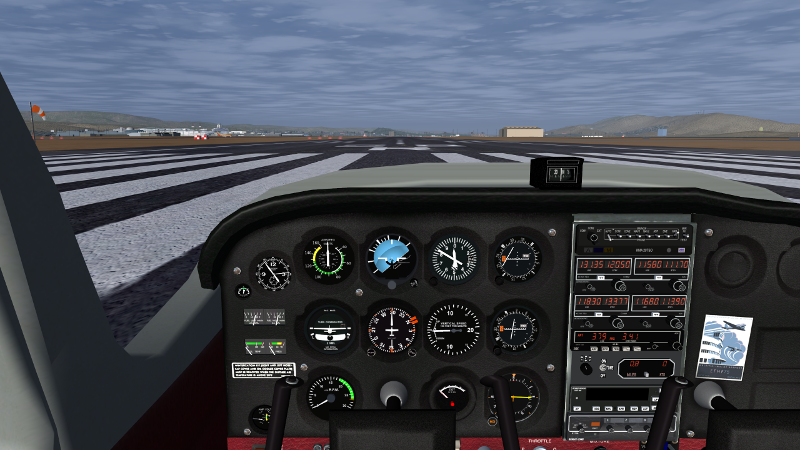
\includegraphics[clip,width=12.5cm]{img/ksfo}
}}
\smallskip
 \noindent

\iflanguage{english}{
Fig.\,3: Ready for takeoff: \textit{Waiting at the default startup position at San Francisco Intl., KSFO.}
}{}
\iflanguage{french}{
Fig.\,3 : Par\'{e} \`{a} d\'{e}coller : \textit{en attente \`{a} la position de d\'{e}marrage par d\'{e}faut de l'a\'{e}roport de San Francisco Intl., KSFO.}
}{}
\medskip

\iflanguage{english}{
Before you can run \FlightGear{}, you need to set a couple of environment variables:
}{}
\iflanguage{french}{
Avant de pouvoir d\'{e}marrer \FlightGear{}, vous devez d\'{e}finir deux variables d'environnement :
}{}

\begin{itemize}
\iflanguage{english}{
\item You must add \texttt{/usr/local/share/FlightGear/lib} to your \texttt{LD\_LIBRARY\_PATH}
\item \texttt{FG\_ROOT} must be set to the data directory of your \FlightGear{} installation. e.g. \texttt{/usr/local/share/FlightGear/data}.
\item \texttt{FG\_SCENERY} should be a list of scenery directories, separated by '':''. This works like \texttt{PATH} when searching for scenery.
e.g. \texttt{\$FG\_ROOT/Scenery:\$FG\_ROOT/WorldScenery}.
}{}

\iflanguage{french}{
\item Vous devez ajouter \texttt{/usr/local/share/FlightGear/lib} \`{a} votre \texttt{LD\_LIBRARY\_PATH}
\item \texttt{FG\_ROOT} doit \^{e}tre param\'{e}tr\'{e} pour pointer vers le r\'{e}pertoire contenant les donn\'{e}es de votre installation de  \FlightGear{}, par exemple : \texttt{/usr/local/share/FlightGear/data}.
\item \texttt{FG\_SCENERY} doit \^{e}tre une liste de r\'{e}pertoires de sc\`{e}nes, s\'{e}par\'{e}s par '':''. Ce fonctionnement est semblable \`{a} celui de \texttt{PATH} lorsqu'on recherche des sc\`{e}nes.
par exemple : \texttt{\$FG\_ROOT/Scenery:\$FG\_ROOT/WorldScenery}.
}{}

\end{itemize}

\noindent
\iflanguage{english}{
To add these in the Bourne shell (and compatibles):
}{}
\iflanguage{french}{
Pour les ajouter dans le Bourne shell (et compatibles) :
}{}
\begin{verbatim}
LD_LIBRARY_PATH=/usr/local/share/FlightGear/lib:$LD_LIBRARY_PATH
export LD_LIBRARY_PATH
FG_HOME=/usr/local/share/FlightGear
export FG_HOME
FG_ROOT=/usr/local/share/FlightGear/data
export FG_ROOT
FG_SCENERY=$FG_ROOT/Scenery:$FG_ROOT/WorldScenery
export FG_SCENERY
\end{verbatim}
\noindent

\iflanguage{english}{
 or in C shell (and compatibles):
}{}
\iflanguage{french}{
 ou en C shell (et compatibles) :
}{}

\begin{verbatim}
setenv LD_LIBRARY_PATH=\
  /usr/local/share/FlightGear/lib:$LD_LIBRARY_PATH
setenv FG_HOME=/usr/local/share/FlightGear
setenv FG_ROOT=/usr/local/share/FlightGear/data
setenv FG_SCENERY=\
  $FG_HOME/Scenery:$FG_ROOT/Scenery:$FG_ROOT/WorldScenery
\end{verbatim}

\iflanguage{english}{
 Once you have these environment variables set up, simply start \FlightGear{} by running
}{}
\iflanguage{french}{
 Une fois que ces variables d'environnement ont \'{e}t\'{e} param\'{e}tr\'{e}es, d\'{e}marrez tout simplement \FlightGear{} en utilisant la commande 
}{}
\texttt{fgfs -$ $-option1 -$ $-option2\dots}
\medskip
\iflanguage{english}{
Command-line options are described in Chapter~\ref{options}.
}{}
\iflanguage{french}{
Les options de ligne de commande sont d\'{e}crites dans le chapitre~\ref{options}.
}{}

%%%%%%%%%%%%%%%%%%%%%%%%%%%%%%%%%%%%%%%%%%%%%%%%%%%%%%%%%%%%%%%%%%%%%%%%%%%%%%%%%%%%%%%%%%%%%%%
\iflanguage{english}{
\section{Launching the simulator under Windows}\index{Launching Flightgear!Windows}\index{Starting Flightgear!Windows}
}{}
\iflanguage{french}{
\section{D\'{e}marrer le simulateur sous Windows}\index{D\'{e}marrer Flightgear!Windows}\index{D\'{e}marrer Flightgear!Windows}
}{}
%%%%%%%%%%%%%%%%%%%%%%%%%%%%%%%%%%%%%%%%%%%%%%%%%%%%%%%%%%%%%%%%%%%%%%%%%%%%%%%%%%%%%%%%%%%%%%%

\iflanguage{english}{
The pre-built windows binaries come complete with a graphical wizard to start \FlightGear{}. Simply double-click on the \texttt{FlightGear Launcher} Start Menu item, or the icon on the Desktop. The launcher allows you to select your aircraft, the start airport and runway, time of day, current weather, and lots
of other settings.
}{}
\iflanguage{french}{
Les binaires pr\'{e}-compil\'{e}s pour Windows sont livr\'{e}s avec un assistant graphique pour d\'{e}marrer \FlightGear{}. Cliquez tout simplement sur l'\'{e}l\'{e}ment \texttt{FlightGear Launcher} du menu D\'{e}marrer, ou double-cliquez sur l'ic\^{o}ne pr\'{e}sente sur le Bureau. L'assistant vous permet de choisir votre a\'{e}ronef, l'a\'{e}roport de d\'{e}marrage et la piste, l'heure du jour, la m\'{e}t\'{e}o en cours, et de nombreux autres param\`{e}tres.
}{}

 \centerline{\fbox{
\includegraphics[clip,width=12.5cm]{launcher}
}}
\smallskip
\noindent

\iflanguage{english}{
Fig.\,4: \textit{The FlightGear Launcher}
}{}
\iflanguage{french}{
Fig.\,4: \textit{L'assistant de d\'{e}marrage de FlightGear}
}{}

\medskip
\iflanguage{english}{
The first time your run it, you will be asked to set your \texttt{FG\_ROOT} variable
(normally \texttt{c:$\backslash$Program Files$\backslash$FlightGear$\backslash$data}) and \texttt{FG\_SCENERY}.
This should be a list of the directories where you have installed scenery, typically
\texttt{c:$\backslash$Program Files$\backslash$FlightGear$\backslash$data$\backslash$Scenery}.

If you set invalid values or change your scenery directories later, you can
change the settings by pressing the ''Prev'' button from the first page of
the launcher.
}{}
\iflanguage{french}{
La premi\`{e}re fois que vous le lancerez, il vous sera demand\'{e} de param\'{e}trer vos variables \texttt{FG\_ROOT}
(g\'{e}n\'{e}ralement \texttt{c:$\backslash$Program Files$\backslash$FlightGear$\backslash$data}) et \texttt{FG\_SCENERY}.
Ce cette derni\`{e}re variable doit contenir une liste de r\'{e}pertoire(s) o\`{u} vous avez install\'{e} des sc\`{e}nes,
typiquement :

\texttt{c:$\backslash$Program Files$\backslash$FlightGear$\backslash$data$\backslash$Scenery}.

Si vous indiquez des valeurs incorrectes ou si vous modifiez les r\'{e}pertoires de vos sc\`{e}nes apr\`{e}s coup, vous pourrez
corriger ces valeurs et appuyant sur le bouton ''Pr\'{e}c\'{e}dent'' \`{a} partir de la premi\`{e}re page de l'assistant.
}{}

\iflanguage{english}{
\subsection{Launching from the command line}
}{}
\iflanguage{french}{
\subsection{Lancement \`{a} partir de la ligne de commande}
}{}

\iflanguage{english}{
Alternatively, you can run FlightGear from the command line. To do this, you
need to set up the \texttt{FG\_ROOT} and \texttt{FG\_SCENERY} environment
variables manually.

Open a command shell, change to the directory where your binary resides
(typically something like
\texttt{c:$\backslash$Program Files$\backslash$FlightGear$\backslash$bin$\backslash$Win32}),
set the environment variables by typing
}{}
\iflanguage{french}{
Alternativement, vous pouvez d\'{e}marrer FlightGear \`{a} partir de la ligne de commande. Pour cela, vous devez param\'{e}trer
les variables d'environnement \texttt{FG\_ROOT} et \texttt{FG\_SCENERY} manuellement.

Ouvrez une invite de commandes, placez-vous dans le r\'{e}pertoire o\`{u} sont positionn\'{e}s vos binaires (g\'{e}n\'{e}ralement quelque chose comme \texttt{c:$\backslash$Program Files$\backslash$FlightGear$\backslash$bin$\backslash$Win32}), puis param\'{e}trez les variables d'environnement en tapant :
}{}

\medskip

\begin{verbatim}
SET FG_HOME="c:\Program Files\FlightGear"
SET FG_ROOT="c:\Program Files\FlightGear\data"
SET FG_SCENERY="c:\Program Files\FlightGear\data\Scenery"
\end{verbatim}
\medskip

\noindent
\iflanguage{english}{
 and invoke \FlightGear{} (within the same Command shell, as environment
 settings are only valid locally within the same shell) via
}{}
\iflanguage{french}{
 et d\'{e}marrez \FlightGear{} (dans la m\^{e}me fen\^{e}tre d'invite de commandes, car les variables d'environnement sont valides
uniquement localement au sein de la m\^{e}me invite de commandes) par l'interm\'{e}diaire de la commande :
}{}
\medskip

\texttt{fgfs -$ $-option1 -$ $-option2\dots}
\medskip
\iflanguage{english}{
Command-line options are described in Chapter~\ref{options}.
Of course, you can create a batch file with a Windows text editor (like notepad)
using the lines above.
For maximum performance it is recommended that you to minimize (iconize) the
text output window while running \FlightGear{}.
}{}
\iflanguage{french}{
Les options de ligne de commande sont d\'{e}crites dans le chapitre~\ref{options}.
Naturellement, vous pouvez cr\'{e}er un fichier \textit{batch} avec un \'{e}diteur de texte Windows (comme le bloc-notes) contenant les lignes ci-dessus.
Pour obtenir les meilleures performances \`{a} l'ex\'{e}cution, il est recommand\'{e} de r\'{e}duire (ic\^{o}nifier) la fen\^{e}tre de sortie pendant que \FlightGear{} est en fonctionnement. 
}{}


%%%%%%%%%%%%%%%%%%%%%%%%%%%%%%%%%%%%%%%%%%%%%%%%%%%%%%%%%%%%%%%%%%%%%%%%%%%%%%%%%%%%%%%%%%%%%%%
\iflanguage{english}{
\section{Launching the simulator under Mac OS X}\index{Launching Flightgear!Mac OS X}\index{Starting Flightgear!Mac OS X}
}{}
\iflanguage{french}{
\section{D\'{e}marrer le simulateur sous Mac OS X}\index{D\'{e}marrer Flightgear!Mac OS X}\index{D\'{e}marrer Flightgear!Mac OS X}
}{}
%%%%%%%%%%%%%%%%%%%%%%%%%%%%%%%%%%%%%%%%%%%%%%%%%%%%%%%%%%%%%%%%%%%%%%%%%%%%%%%%%%%%%%%%%%%%%%%
\iflanguage{english}{
The prebuilt binary package for Mac OS X comes with the GUI launcher. Simply double-click the \FlightGear{} icon on /Applications folder shows up the GUI launcher window as shown in Fig. 5. The launcher allows you to :

\begin{itemize}
\item Select an aircraft and an airport
\item Enable/Disable automatic scenery download (using \TerraSync{})
\item Enable/Disable the Navigation Map (Atlas)
\item Launch \FlightGear{}
\end{itemize}

The following sections describe the use of these features.
}{}

\iflanguage{french}{
Le paquetage de binaires pr\'{e}-compil\'{e}s pour Mac OS X est livr\'{e} avec un assistant en mode graphique. Double-cliquez simplement sur l'ic\^{o}ne \FlightGear{} dans le dossier /Applications pour lancer la fen\^{e}tre GUI launcher comme d\'{e}montr\'{e} \`{a} la Fig. 5. L'assistant vous permet :

\begin{itemize}
\item de choisir un a\'{e}ronef et un a\'{e}roport
\item d'activer/d\'{e}sactiver le t\'{e}l\'{e}chargement automatique des sc\`{e}nes (en utilisant \TerraSync{})
\item d'activer/d\'{e}sactiver la carte de navigation (Atlas)
\item de d\'{e}marrer \FlightGear{}
\end{itemize}

Les sections suivantes d\'{e}crivent l'utilisation de ces fonctionnalit\'{e}s.
}{}
\smallskip
\centerline{\fbox{
\includegraphics[clip,width=12.5cm]{img/maclauncher}
}}
\smallskip
\noindent
\iflanguage{english}{
Fig.\,5: \textit{The GUI Launcher for Mac OS X} \label{fig:maclauncher}
}{}
\iflanguage{french}{
Fig.\,5: \textit{L'assistant graphique pour Mac OS X} \label{fig:maclauncher}
}{}

\medskip

\iflanguage{english}{
\subsection{Selecting an aircraft and an airport}
At the launcher window, you can select an aircraft and an airport by clicking gear buttons at the right end of the airport/aircraft name. The thumbnail image of a selected aircraft will show up at the image panel on the window. The airport that you select here will be the starting point of your flight. \FlightGear{} uses ICAO 4-letter airport code, which is composed with one or two prefix letters followed by a two or three letter airport code. For example, the ICAO code for San Francisco International Airport is KSFO. ``K'' in this case is the prefix for The United States, and SFO is the airport code for San Francisco International Airport. You can use \textit{Advanced features >> Position} or \textit{Aircraft} tab to find an airport or an aircraft.
}{}
\iflanguage{french}{
\subsection{Choisir un a\'{e}ronef et un a\'{e}roport}
Dans la fen\^{e}tre de l'assistant, vous pouvez choisir un a\'{e}ronef et un a\'{e}roport en cliquant sur les boutons situ\'{e}s \`{a} droite du nom de l'a\'{e}roport/a\'{e}ronef. L'image miniature de l'a\'{e}ronef s\'{e}lectionn\'{e} s'affichera dans le panneau image de la fen\^{e}tre. L'a\'{e}roport que vous choisissez ici sera le point de d\'{e}part de votre vol. \FlightGear{} utilise les codes a\'{e}roport \`{a} quatre lettres de l'OACI, qui se compose d'une ou deux lettres de pr\'{e}fixe, suivies de une ou deux lettres correspondant au code a\'{e}roport. Par exemple, le code OACI de l'a\'{e}roport international de San Francisco est KSFO. Dans cet exemple, ``K'' est le pr\'{e}fixe pour les Etats-Unis, et SFO est le code a\'{e}roport pour l'a\'{e}roport international de San Francisco. Vous pouvez utiliser l'onglet \textit{Fonctionnalit\'{e}s avanc\'{e}es >> Position} ou \textit{A\'{e}ronef} pour trouver un a\'{e}roport ou un a\'{e}ronef.
}{}

\iflanguage{english}{
\subsection{Enabling on-the-fly scenery downloading}
By checking \textit{Download scenery on the fly} at the launcher window, the scenery data will be downloaded while you're flying using \TerraSync{}. The scenery downloader will install the scenery data into \\
}{}
\iflanguage{french}{
\subsection{Activer le t\'{e}l\'{e}chargement des sc\`{e}nes \`{a} la vol\'{e}e}
En activant \textit{T\'{e}l\'{e}charger les sc\`{e}nes \`{a} la vol\`{e}e} dans la fen\^{e}tre de l'assistant, les donn\'{e}es des sc\`{e}nes seront t\'{e}l\'{e}charg\'{e}es pendant que vous volez grace \'{a} \TerraSync{}. L'outil de t\'{e}l\'{e}chargement des scenes installera ces donn\'{e}es dans le r\'{e}pertoire \\
}{}

\texttt{/Applications/FlightGear.app/Contents/Resouces/data/Scenery-Terrasync}. 

\iflanguage{english}{
\subsection{Enabling Navigation Map (Atlas)}
The Mac version of \FlightGear{} includes Atlas, the navigation map that helps your flight plan, for your convenience. Checking this option will automatically launch Atlas when you start the flight. You don't have to specify any Atlas options. The GUI launcher will specify these for you.
}{}
\iflanguage{french}{
\subsection{Activer la carte de navigation (Atlas)}
La version Mac de \FlightGear{} comprend Atlas, la carte de navigation qui vous aide \`{a} suivre votre plan de vol, pour votre confort. L'activation de cette option lancera automatiquement Atlas lorsque vous d\'{e}marrerez votre vol. Vous n'avez pas besoin de sp\'{e}cifier d'options Atlas. L'assistant graphique les pr\'{e}cisera pour vous.
}{}

\iflanguage{english}{
\subsection{Launching FlightGear - the simulator}
Clicking \textit{Start Flight} button at the launcher window opens up another window - the FlightGear main window. \FlightGear{} immediately starts loading tons of data required for simulation. It may take a while on slower machines to load everything.
}{}
\iflanguage{french}{
\subsection{D\'{e}marrer FlightGear - le simulateur}
Cliquer sur le bouton \textit{D\'{e}marrer le vol} dans la fen\^{e}tre de l'assistant ouvre une nouvelle fen\^{e}tre - la fen\^{e}tre principale de FlightGear. \FlightGear{} d\'{e}marre imm\'{e}diatement le chargement des tonnes de donn\'{e}es n\'{e}cessaires pour la simulation. Le temps de chargement peut \^{e}tre un peu long sur des machines lentes.
}{}

\iflanguage{english}{
\subsection{Advanced Features}
\FlightGear{} has many features and options that you can specify at launch time. Some of these are not changeable from the menu in the \FlightGear{} main window. To enable / disable these features, click the triangle-shaped button at the left-bottom of the launcher window. This displays the advanced features tabs. All settings are saved so you don't have to respecify them.
}{}

\iflanguage{french}{
\subsection{Fonctionnalit\'{e}s avanc\'{e}es}
\FlightGear{} poss\`{e}de de nombreuses fonctionnalit\'{e}s et options que vous pouvez sp\'{e}cifier lors du d\'{e}marrage. Quelques-unes d'entre elles ne peuvent pas \^{e}tre modifi\'{e}es \`{a} partir du menu de la fen\^{e}tre principale de \FlightGear{}. Pour activer/d\'{e}sactiver ces fonctionnalit\'{e}s, cliquez sur le bouton en forme de triangle dans l'angle inf\'{e}rieur gauche de la fen\^{e}tre de l'assistant. Ceci affiche l'onglet fonctionnalit\'{e}s avanc\'{e}es. Tous les param\`{e}tres sont sauvegard\'{e}s de mani\`{e}re \`{a} ce que vous n'ayez pas \`{a} les resp\'{e}cifier \`{a} chaque fois.
}{}

\iflanguage{english}{
\subsubsection{General, Features, and Rendering tabs}
These tabs let you specify some of \FlightGear{} options:
\begin{itemize}
\item \textbf{Save preferences on exit:} lets \FlightGear{} save preferences that you changed from the menu in the \FlightGear{} (fgfs) main window will be saved to \\ \texttt{\$HOME/.fgfs/autosave.xml}.
\item \textbf{Control:} specifies the control device you will use in \FlightGear{}. \textit{auto, joystick, mouse, and keyboard} are available. You can leave it as \textit{auto} unless you really want to change it manually.
\item \textbf{Unit:} specifies the unit used in \FlightGear{}. \textit{feet} and \textit{meters} are available.
\item \textbf{Time of day:} specifies the time of day. Available options are \textit{real, dawn, morning, noon, afternoon, dusk, evening, and midnight}.
\item \textbf{Season:} specifies the season of \FlightGear{} world. You can choose either summer or winter.
\item \textbf{Sound:} disabling this will cut all the sound in FlightGear.
\item \textbf{Instrumental panel:} specifies if 2D panel is drawn from the beginning. You can also enable/disable the 2D panel from \FlightGear{} menu.
\item \textbf{Random objects:} specifies whether \FlightGear{} draws random objects or not.
\item \textbf{AI models:} specifies whether \FlightGear{} handles AI aircraft and ships.
\item \textbf{Clock never advances:} specifies whether the clock advances in \FlightGear{} or not.
\item \textbf{No fuel consumption:} makes aircraft consume no fuel while it's flying.
\item \textbf{Start in a frozen state:} starts \FlightGear{} with frozen state. it does not seem working at this moment.
\item \textbf{Display HUD:} displays HUD at the beginning, I guess. You can turn HUD on/off by pressing 'h' while you are flying.
\item \textbf{3D HUD:} enables 3D HUD if an selected aircraft supports it.
\item \textbf{Real weather fetch:} enables fetching real weather condition using METAR.
\item \textbf{Horizon effect:} enables horizon effect.
\item \textbf{Clouds:} enables drawing clouds.
\item \textbf{3D clouds:} enables drawing 3D clouds. You need to enable 3D clouds by checking \textit{3D cloud} from the \textit{View >> Rendering option} on the \FlightGear{} simulator window. 
\item \textbf{Turbulence:} specifies the strength of turbulence. 0.0 is calm and 1.0 is severe. You need to specify value from 0.0 through 1.0
\item \textbf{Visibility:} specifies the visibility in meter. You can specify 5000 or less if \FlightGear{} runs slow on your machine.
\item \textbf{Fullscreen mode:} enabling this will launch \FlightGear{} as full-screen mode.
\item \textbf{Window size:} specifies the size of \FlightGear{} window. It will be ignored when full-screen mode is enabled.
\item \textbf{Sky blending:} enables or disables \FlightGear{} to blend the sky depending on time and surrounding environment. DO NOT disable this option, or \FlightGear{} crashes.
\item \textbf{Textures:} enables or disables textures on runways, buildings, and scenery objects. Disabling this will give you some more fps, effective especially on G4 Macs.
\item \textbf{Wireframe:} lets \FlightGear{} draw wire-frames so you can see how the world of \FlightGear{} is drawn. This should be enabled only for debug / development purpose.
\item \textbf{Fog:} specifies how fog is drawn. \textit{disable, fastest, nicest} are available.
\end{itemize}
}{}

\iflanguage{french}{
\subsubsection{Onglets G\'{e}n\'{e}ralit\'{e}s, Fonctionnalit\'{e}s et Rendu}
Ces onglets vous permettent de d\'{e}finir certaines options de \FlightGear{} :
\begin{itemize}
\item \textbf{Sauvegarder les pr\'{e}f\'{e}rences \`{a} la fermeture :} permet \`{a} \FlightGear{} de sauvegarder les pr\'{e}f\'{e}rences que vous avez modifi\'{e}es \`{a} partir du menu dans la fen\^{e}tre principale de \FlightGear{} (fgfs) vers le fichier \\ \texttt{\$HOME/.fgfs/autosave.xml}.
\item \textbf{Contr\^{o}les :} pr\'{e}cise le moyen de contr\^{o}le que vous utiliserez dans \FlightGear{}. \textit{auto, joystick, souris et clavier} sont disponibles. Vous pouvez conserver ce param\`{e}tre en mode \textit{auto} sauf si vous tenez \`{a} le param\'{e}trer manuellement.
\item \textbf{Unit\'{e}s :} d\'{e}finit l'unit\'{e} utilis\'{e}e dans \FlightGear{}. Les \textit{pieds} et les \textit{m\`{e}tres} sont disponibles.
\item \textbf{Heure du jour :} fixe l'heure du jour. Les options disponibles sont \textit{r\'{e}elle, aube, matin, midi, apr\`{e}s-midi, cr\'{e}puscule, soir et minuit}.
\item \textbf{Saison :} d\'{e}finit la saison du monde \FlightGear{}. Vous pouvez choisir \'{e}t\'{e} ou hiver.
\item \textbf{Son :} la d\'{e}sactivation de cette option coupera le son dans FlightGear.
\item \textbf{Panneaux d'instruments :} pr\'{e}cise si un panneau 2D est activ\'{e} par d\'{e}faut. Vous pouvez \'{e}galement activer/d\'{e}sactiver le panneau 2D \`{a} partir du menu \FlightGear{}.
\item \textbf{Objets al\'{e}atoires :} pr\'{e}cise si \FlightGear{} affichera des objets al\'{e}atoires ou non.
\item \textbf{Mod\`{e}les IA :} pr\'{e}cise si \FlightGear{} g\`{e}rera les a\'{e}ronefs et navires IA.
\item \textbf{L'horloge n'avance jamais :} d\'{e}finit si l'horloge avance dans \FlightGear{} ou non.
\item \textbf{Pas de consommation de carburant :} laisse l'avion ne consommer aucun carburant lorsqu'il vole.
\item \textbf{D\'{e}marrer dans un \'{e}tat fig\'{e} :} d\'{e}marre \FlightGear{} dans un \'{e}tat fig\'{e}. Cette option a l'air de ne pas fonctionner actuellement.
\item \textbf{Activer l'affichage t\^{e}te haute (HUD) :} affiche le HUD au d\'{e}marrage, je pense. Vous pouvez activer/d\'{e}sactiver le HUD en appuyant sur 'h' lorsque vous volez.
\item \textbf{HUD 3D :} active le HUD 3D si un avion s\'{e}lectionn\'{e} le prend en charge.
\item \textbf{M\'{e}t\'{e}o r\'{e}elle :} active la r\'{e}cup\'{e}ration des conditions m\'{e}t\'{e}o r\'{e}elles en utilisant les METAR.
\item \textbf{Effet de l'horizon :} active l'effet de l'horizon.
\item \textbf{Nuages :} active l'affichage des nuages.
\item \textbf{Nuages 3D :} active l'affichage des nuages 3D. Vous devrez activer les nuages 3D en activant la case \textit{Nuages 3D} dans le menu \textit{Affichage >> Options de rendu} dans la fen\^{e}tre du simulateur \FlightGear{}. 
\item \textbf{Turbulence :} pr\'{e}cise la force des turbulences en vol. 0.0 est calme et 1.0 est forte. Vous devez sp\'{e}cifier une valeur allant de 0.0 \`{a} 1.0.
\item \textbf{Visibilit\'{e} :} sp\'{e}cifie la visibilit\'{e} en m\`{e}tres. Vous pouvez donner une valeur de 5 000 ou moins si \FlightGear{} tourne lentement sur votre machine.
\item \textbf{Mode plein \'{e}cran :} l'activation de ce param\`{e}tre lancera \FlightGear{} en mode plein \'{e}cran.
\item \textbf{Taille de la fen\^{e}tre :} d\'{e}finit la taille de la fen\^{e}tre \FlightGear{}. Sera ignor\'{e} si le mode plein \'{e}cran est activ\'{e}.
\item \textbf{Fondu du ciel :} active ou d\'{e}sactive le fondu du ciel dans \FlightGear{} en fonction du temps et de l'environnement proche. NE DESACTIVEZ PAS cette option, sous peine de voir \FlightGear{} dysfonctionner.
\item \textbf{Textures :} active ou d\'{e}sactive les textures sur les pistes, les immeubles et les objets des sc\`{e}nes. La d\'{e}sactivation vous donnera quelques images par seconde en plus, sp\'{e}cialement sur les Macs G4.
\item \textbf{Fil de fer :} demande \`{a} \FlightGear{} de dessiner le monde en fils de fer, de telle sorte que vous puissiez visualiser la mani\`{e}re dont le monde de \FlightGear{} est rendu. Ceci ne devrait \^{e}tre activ\'{e} que pour des besoins de d\'{e}bogage ou de d\'{e}veloppement.
\item \textbf{Brouillard :} pr\'{e}cise la mani\`{e}re dont le brouillard est rendu. \textit{d\'{e}sactiv\'{e}, plus rapide, plus beau} sont les options disponibles.
\end{itemize}
}{}

\iflanguage{english}{
\subsubsection{Favorite tab}
Favorite list provides a means of preserving a named set of current options like a book mark of a web browser. To save the current set of options, press ``+'' button on the top window or at the bottom of the Favorite tab. Once favorites are added, You can switch from one configuration to another by double-clicking a row in the table view in the Favorite tab. Pressing ``-'' button (or delete key) on a favorite in the table view deletes the selected favorite.
}{}
\iflanguage{french}{
\subsubsection{Onglet Favoris}
La liste des favoris offre un moyen de conserver un \'{e}tat nomm\'{e} des options actuelles, \`{a} la fa\c{c}on du marque-pages d'un navigateur Internet. Pour sauvegarder l'\'{e}tat actuel des options, appuyez sur le bouton ``+'' dans le haut de la fen\^{e}tre ou en-bas de l'onglet Favoris. Une fois que les favoris ont \'{e}t\'{e} ajout\'{e}s, vous pouvez basculer d'une configuration \`{a} l'autre en double-cliquant sur une ligne du tableau dans l'onglet Favoris. L'appui sur le bouton ``-'' (ou sur la touche suppression) sur un favori dans le tableau efface le favori s\'{e}lectionn\'{e}.
}{}

\subsubsection{Position}
\iflanguage{english}{
You can find airports or aircraft carriers by searching with a keyword into the filter text area. Available keywords are:
}{}
\iflanguage{french}{
Vous pouvez trouver des a\'{e}roports ou des porte-avions en cherchant en utilisant une recherche par mot-cl\'{e} dans la zone de texte filtre. Les mots-cl\'{e}s disponibles sont :
}{}

\begin{itemize}
\iflanguage{english}{
\item For airports:
	\begin {itemize} 
	\item a part of airport name (e.g. international, ranch, or civil),
	\item country name (such as Japan, USA, or France) if available,
	\item location name (such as city or county or U.S. state abbrev. if available),
	\item IATA code (such as SFO, LAX, HND) if available,
	\item ICAO code (such as KSFO, KLAX, RJTT) - works on all airports.
	\end{itemize}
\item For aircraft carriers:
	\begin{itemize}
	\item carrier name (Nimitz or Eisenhower),
	\item ``carrier''.
	\end{itemize}
}{}
\iflanguage{french}{
\item Pour les a\'{e}roports :
	\begin {itemize} 
	\item une partie du nom de l'a\'{e}roport (par exemple : international, ranch, ou civil),
	\item le nom du pays (comme Japon, USA, ou France) si connu,
	\item le nom de l'emplacement (comme la ville ou le nom abbr\'{e}g\'{e} de l'\'{e}tat aux Etats-Unis),
	\item code IATA (comme SFO, LAX, HND) si disponible,
	\item code OACI (comme KSFO, KLAX, RJTT) - fonctionne pour tous les a\'{e}roports.
	\end{itemize}
\item Pour les porte-avions :
	\begin{itemize}
	\item nom du porte-avions (Nimitz ou Eisenhower),
	\item ``carrier''.
	\end{itemize}
}{}

\end{itemize}

\iflanguage{english}{
Airports and carriers that match the keyword are shown at the table view below the filter text area. The airport name at the upper pane is synchronized with the currently selected airport or carrier. You can also open this tab by clicking the gear button at the right end of airport name on the top pane.
When you choose an airport, available runways show up at the ``runway'' pop-up button. You can choose a runway or leave it as ``default.''
}{}
\iflanguage{french}{
Les a\'{e}roports et les porte-avions qui correspondent au mot-cl\'{e} sont affich\'{e}s dans la vue du tableau sous la zone de texte filtre. Vous pouvez \'{e}galement ouvrir cet onglet en cliquant sur le bouton situ\'{e} \`{a} l'extr\'{e}mit\'{e} droite du nom de l'a\'{e}roport sur le panneau sup\'{e}rieur.
Lorsque vous choisissez un a\'{e}roport, les pistes disponibles s'affichent dans le bouton pop-up ``piste''. Vous pouvez choisir une piste ou le laisser sur ``d\'{e}faut.''
}{}

\iflanguage{english}{
\subsubsection{Aircraft tab}
You can find aircraft by searching with a keyword into the filter text area. Available keywords are:
}{}
\iflanguage{french}{
\subsubsection{Onglet A\'{e}ronefs}
Vous pouvez trouver les a\'{e}ronefs en cherchant avec un mot cl\'{e} dans la zone de texte filtre. Les mot-cl\'{e}s disponibles sont :
}{}

\iflanguage{english}{
\begin{itemize}
\item a part of aircraft name (e.g. c172, zero, shinden)
\item configuration file name without -set.xml (e.g. a6m2, p51d)
\item fdm (Flight Dynamics Model) name (e.g. yasim, jsb)
\item status (e.g. alpha, beta, production, development)
\end{itemize}
A list of aircraft that match the keyword shows up at the table view below the filter text area. The aircraft name at the upper pane is synchronized with the currently selected aircraft. You can also open this tab by clicking the gear button at the right end of aircraft name on the top pane.

If you want to find more aircraft data from the internet, click ``Get Aircraft'' button at the bottom of the Aircraft tab. It opens a web browser to lead you to the Aircraft Links page on \textit{FlightGear Mac OS X} web site. You can visit some links there and download an aircraft you want. Once an aircraft is downloaded, open ``Others'' tab to install it. 

If you encounter some weird behavior in searching aircraft, removing a cache file for aircraft database might solve your problem. Open \\ \texttt{/Applications/Utilities/Terminal.app} and type the following commands to remove the cache file:
}{}
\iflanguage{french}{
\begin{itemize}
\item une partie du nom de l'a\'{e}ronef (par exemple : c172, zero, shinden)
\item le nom d'un fichier de configuration sans le -set.xml (par exemple : a6m2, p51d)
\item le nom du FDM (Mod\`{e}le de dynamique de vol) (par exemple : yasim, jsb)
\item le statut (par exemple : alpha, beta, production, d\'{e}veloppement)
\end{itemize}
Une liste des a\'{e}ronefs correspondant au mot cl\'{e} s'affichent dans la vue du tableau sous la zone de texte filtre. Le nom d'a\'{e}ronef sur le panneau sup\'{e}rieur est synchronis\'{e} avec l'a\'{e}ronef actuellement s\'{e}lectionn\'{e}. Vous pouvez \'{e}galement ouvrir cet onglet en cliquant sur le bouton situ\'{e} \`{a} l'extr\'{e}mit\'{e} droite du nom de l'avion sur le panneau sup\'{e}rieur.

Si vous voulez trouver plus d'a\'{e}ronefs \`{a} partir d'Internet, cliquez sur le boutou ``Obtenir des a\'{e}ronefs'' en bas de l'onglet A\'{e}ronefs. Ceci ouvrira un navigateur pour vous mener \`{a} la page Liens A\'{e}ronefs sur le site Internet \textit{FlightGear Mac OS X}. Vous pouvez consulter certains liens qui s'y trouvent et t\'{e}l\'{e}charger l'a\'{e}ronef que vous souhaitez. Une fois que l'a\'{e}ronef est t\'{e}l\'{e}charg\'{e}, ouvrez l'onglet ``Autres'' pour l'installer. 

Si vous constatez un comportement anormal lorsque vous recherchez un a\'{e}ronef, supprimer un fichier de cache de la base de donn\'{e}es des a\'{e}ronefs peut r\'{e}soudre votre probl\`{e}me. Ouvrez \\ \texttt{/Applications/Utilities/Terminal.app} et tapez les commandes suivantes pour supprimer le fichier de cache :
}{}

\begin{verbatim}
  cd /Applications/FlightGear.app/Contents/Resources
  rm AircraftCache.rb
\end{verbatim}

\medskip
\iflanguage{english}{
Note that you must not launch \FlightGear{} from mounted disk image of a prebuilt binary package since the folder in the mounted disk image is read-only, which prevents you from installing any add-on data. Vou need to install \FlightGear{} by copying the \FlightGear{} icon from the mounted disk image to \texttt{/Applications} folder.
}{}
\iflanguage{french}{
Notez que vous ne devez pas lancer \FlightGear{} \`{a} partir de l'image disque d'un paquetage binaire pr\'{e}compil\'{e} car le r\'{e}pertoire de l'image disque mont\'{e}e est en lecture seule, ce qui vous emp\^{e}che d'installer toute donn\'{e}e ajout\'{e}e. Vous devez installer \FlightGear{} en copiant l'ic\^{o}ne \FlightGear{} depuis l'image disque mont\'{e}e vers le r\'{e}pertoire \texttt{/Applications}.
}{}

\iflanguage{english}{
\subsubsection{Network tab}
This tab contains two network features of \FlightGear{}. One is multi-player mode and another is FGCOM (a voice ATC). To enable multi-player mode, specify the followings:
\begin{itemize}
\item \textbf{Enable Multiplay:} enables or disables multi-player mode. Enabling this will open a new browser window to show the map on a multi player server.
\item \textbf{Callsign:} specifies the name shown in the map. Username must contain only alphabet letters, numbers, underscores, and dots. \FlightGear{} will exit when you specify a call sign with invalid characters. A user name with 8 or more characters will be truncated into the first 7 characters. 
\item \textbf{Server:} specifies the server to connect. \texttt{mpserver02.flightgear.org} is available at the time of writing this.
\item \textbf{Your Mac:} specifies your Mac's IP address. Usually the launcher detects the address automatically. If something is wrong with network connection, clear this text field.
\item \textbf{Port:} must be 5000
\end{itemize}

FGCOM enables you to make a real voice communication using radio setting. You can talk at a selected radio frequency (COM1) while pressing space bar. You can listen to some other player's talking in the frequency if some others are using the same frequency and you are in range. The options available for FGCOM are listed below:

\begin{itemize}
\item \textbf{Enable FGCOM in Multi Player mode:} specifies if you use FGCOM when Multiplay is enabled.
\item \textbf{FGCOM Server:} specifies a VOIP server.
\end{itemize}

For further instructions on FGCOM, and Multiplay, please see Chapter \ref{features}.
}{}

\iflanguage{french}{
\subsubsection{Onglet r\'{e}seau}
Cet onglet contient deux fonctionnalit\'{e}s r\'{e}seau de \FlightGear{}. L'une est le mode multijoueurs et l'autre est FGCOM (un syst\`{e}me de contr\^{o}le a\'{e}rien vocal). Pour activer le mode multijoueurs, pr\'{e}cisez les items suivants :
\begin{itemize}
\item \textbf{Activer le mode multijoueurs :} active ou d\'{e}sactive le mode multijoueurs. L'activation ouvrira une nouvelle fen\^{e}tre du navigateur pour afficher la carte sur un serveur multijoueurs.
\item \textbf{Indicatif :} pr\'{e}cise le nom affich\'{e} sur la carte. Un nom d'utilisateur peut contenir des lettres de l'alphabet, des nombres, des tirets-bas (\textit{underscores}) et des points. \FlightGear{} se terminera si vous pr\'{e}cisez un indicatif avec des caract\`{e}res invalides. Un nom d'utilisateur contenant 8 caract\`{e}res ou plus sera tronqu\'{e} avec les seuls 7 premiers caract\`{e}res. 
\item \textbf{Serveur :} pr\'{e}cise le serveur auquel se connecter. \texttt{mpserver02.flightgear.org} est disponible \`{a} l'heure de l'\'{e}criture de ce document.
\item \textbf{Votre Mac :} d\'{e}finit l'adresse IP de votre Mac. G\'{e}n\'{e}ralement, l'assistant d\'{e}tecte l'adresse de mani\`{e}re automatique. Si quelque chose n'est pas exact avec votre connection r\'{e}seau, effacez le contenu de ce champ texte.
\item \textbf{Port :} doit \^{e}tre \'{e}gal \`{a} 5000.
\end{itemize}

FGCOM vous permet d'effectuer une v\'{e}ritable communication audio en utilisant des param\`{e}tres radio. Vous pouvez parler sur une fr\'{e}quence radio pr\'{e}cise (COM1) en appuyant sur la barre d'espace. Vous pouvez \'{e}coutez d'autres joueurs parlant sur la fr\'{e}quence si d'autres joueurs sont sur cette fr\'{e}quence et que vous \^{e}tes \`{a} leur port\'{e}e. Les options pour FGCOM sont list\'{e}es ci-dessous :

\begin{itemize}
\item \textbf{Active FGCOM en mode multijoueurs :} indique si vous utilisez FGCOM lorsque le mode multijoueurs est activ\'{e}.
\item \textbf{Serveur FGCOM :} pr\'{e}cise un serveur VOIP.
\end{itemize}

Des informations compl\'{e}mentaires concernant FGCOM et le mode multijoueurs sont disponibles au chapitre \ref{features}.
}{}

\iflanguage{english}{
\subsubsection{Others tab}
You can specify any options other than aircraft, airport, and the options shown in the launcher. Entering space-separated options as shown in Figure 11 will pass additional options to \FlightGear{}. You can see all available options by pressing ``View Options.'' Some options might cause \FlightGear{} crash. If you encounter such crashes with a specific option, please let us know.

To install additional aircraft and scenery data, press "Install Add-on Data." You can specify multiple files and/or folders to install to the \FlightGear{} data folder. Acceptable file types are:
\begin{itemize}
\item zip
\item tar
\item tar.gz
\item tar.bz2
\item folder
\item 7zip (only if 7zip is installed)
\end{itemize}

You will see the message window when all the data is successfully installed, otherwise error message will show up. You can select both aircraft and scenery data at the same time. If you select an archived file that does not contain aircraft files, it will be extracted into the data folder, but will be ignored. When you finish installing new aircraft, you can select the aircraft on the ``Aircraft'' tab.
}{}
\iflanguage{french}{
\subsubsection{Onglet Autres}
Vous pouvez pr\'{e}ciser toutes les options autres que a\'{e}ronef, a\'{e}roport et les options affich\'{e}es dans l'assistant. En entrant des options s\'{e}par\'{e}es par des espaces comme pr\'{e}sent\'{e} \`{a} la Figure 11, vous passerez des options additionnelles \`{a} \FlightGear{}. Vous pouvez voir toutes les options disponibles en appuyant sur ``Voir Options.'' Certaines options peuvent faire dysfonctionner \FlightGear{}. Si vous rencontrez de tels dysfonctionnements avec une option particuli\`{e}re, merci de nous le signaler.

Pour installer des a\'{e}ronefs et des sc\`{e}nes additionnelles, appuyez sur "Installer des donn\'{e}es additionnelles." Vous pouvez pr\'{e}ciser les fichiers ou r\'{e}pertoires multiples \`{a} installer dans le r\'{e}pertoire des donn\'{e}es \FlightGear{}. Les types de fichiers accept\'{e}s sont :
\begin{itemize}
\item zip
\item tar
\item tar.gz
\item tar.bz2
\item dossier
\item 7zip (seulement si 7zip est install\'{e})
\end{itemize}

Vous verrez la fen\^{e}tre d'information lorsque toutes les donn\'{e}es ont \'{e}t\'{e} correctement install\'{e}es, dans le cas contraire les messages d'erreurs y seront affich\'{e}s. Vous pouvez choisir des donn\'{e}es d'a\'{e}ronefs et de sc\`{e}nes en m\^{e}me temps. Si vous choisissez un fichier archiv\'{e} qui ne contient pas de fichiers d'a\'{e}ronefs, il sera extrait dans le r\'{e}pertoire des donn\'{e}es, mais sera ignor\'{e}. Lorsque vous aurez termin\'{e} l'installation d'un nouvel a\'{e}ronef, vous pouvez choisir l'a\'{e}ronef concern\'{e} dans l'onglet ``A\'{e}ronefs''.
}{}

\iflanguage{english}{
\subsection{Launching from the command line}
You can also launch the simulator from the command line on Mac OS X. To do so, open Terminal.app (located at \texttt{/Applications/Utilities}) and type the following commands:
}{}
\iflanguage{french}{
\subsection{D\'{e}marrage \`{a} partir de la ligne de commande}
Vous pouvez \'{e}galement d\'{e}marrer le simulateur \`{a} partir de la ligne de commande sur Mac OS X. Pour le faire, ouvrez Terminal.app (situ\'{e} dans \texttt{/Applications/Utilitaires}) et tapez les commandes suivantes :
}{}

\begin{verbatim}
  cd /Applications/FlightGear.app/Contents/Resources
  ./fgfs --option1 --option2 ....
\end{verbatim}

\iflanguage{english}{
See chapter \ref{options} for detail information on command line options. Unlike the other platforms, you don't have to manually specify the environment variables such as FG\_ROOT and FG\_SCENERY as long as you use a prebuilt binary package.
}{}
\iflanguage{french}{
Reportez-vous au chapitre \ref{options} pour obtenir plus d'informations d\'{e}taill\'{e}es sur les options en ligne de commande. Contrairement aux autres plate-formes, vous n'avez pas besoin de pr\'{e}ciser manuellement les variables d'environnement comme FG\_ROOT et FG\_SCENERY tant que vous utilisez un paquetage binaire pr\'{e}compil\'{e}.
}{}

%%%%%%%%%%%%%%%%%%%%%%%%%%%%%%%%%%%%%%%%%%%%%%%%%%%%%%%%%%%%%%%%%%%%%%%%%%%%%%%%%%%%%%%%%%%%%%%
\section{Command line parameters\label{options}}\index{command line options}
%%%%%%%%%%%%%%%%%%%%%%%%%%%%%%%%%%%%%%%%%%%%%%%%%%%%%%%%%%%%%%%%%%%%%%%%%%%%%%%%%%%%%%%%%%%%%%%
Following is a complete list and short description of the numerous \Index{command line options}
available for \FlightGear{}. Most of these options are exposed through the \FlightGear{} launcher delivered with the
Windows binaries.

If you have options you re-use continually, you can create a preferences file
containing a set of command-line options that will be set automatically. You
can create the file with any text editor (notepad, emacs, vi, if you like).

\begin{itemize}
\item On Unix systems (including Mac OS X), put the command line options in a
file called \texttt{.fgfsrc}\index{.fgfsrc} in your home directory.

\item On Windows, put the command line options in a file called \texttt{system.fgfsrc}
\index{system.fgfsrc} in the \texttt{FG\_ROOT} directory (e.g. \texttt{c:$\backslash$Program Files$\backslash$FlightGear$\backslash$data}).
\end{itemize}

%%%%%%%%%%%%%%%%%%%%%%%%%%%%%%%%%%%%%%%%%%%%%%%%%%%%%%%%%%%%%%%%%%%%%%%%%%%%%%%%%%%%%%%%%%%%%%%
\subsection{General Options}\index{options!general}\label{generaloptions}
%%%%%%%%%%%%%%%%%%%%%%%%%%%%%%%%%%%%%%%%%%%%%%%%%%%%%%%%%%%%%%%%%%%%%%%%%%%%%%%%%%%%%%%%%%%%%%%
\begin{itemize}
\item{\texttt{-$ $-help}}

  Display the most relevant command line options.

\item{\texttt{-$ $-help} \texttt{-$ $-verbose}}

  Display all command line options.

\item{\texttt{-$ $-language={\it code}}}

  Select the language for this session. e.g. pl, nl, it, fr, en, de.

\item{\texttt{-$ $-version} }

Display the current \FlightGear{} version.

\item{\texttt{-$ $-fg-root={\it path}}}

  Tells \FlightGear{} where to look for its root data files if you
  didn't compile it with the \Index{default settings}.

\item{\texttt{-$ $-fg-scenery={\it path}}}

  Allows specification of a path to the base scenery path
  \index{scenery directory!path}, in case scenery is not at the default
  position under \texttt{\$FG\underline{~}ROOT/Scenery}; this might
  be especially useful in case you have scenery on a CD-ROM.

\item{\texttt{-$ $-enable-save-on-exit}, \texttt{-$ $-disable-save-on-exit}}

  Enable or disable saving of user-preferences on exit from the simulator.

\item{\texttt{-$ $-enable-freeze}, \texttt{-$ $-disable-freeze}}

  Control whether \FlightGear{} starts paused or not. Defaults to not paused.

\item{\texttt{-$ $-control={\it mode}}}

  Specify your primary \Index{control mode} (\Index{\texttt{joystick}},  \texttt{keyboard},
  \texttt{mouse}) Defaults to \Index{joystick}.

\item{\texttt{-$ $-enable-auto-coordination}, \texttt{-$ $-disable-auto-coordination}}

  Switches \Index{auto-co-ordination} between aileron and rudder on/off. Auto-coordination
  is recommended for users without rudder pedals or a `twist' joystick. Defaults to off.

\item{\texttt{-$ $-browser-app={\it path}}}

  Specify location of your web browser. E.g:
  \texttt{-$ $-browser-app=}\\
  \texttt{``C:$\backslash$Program~Files$\backslash$Internet~Explorer$\backslash$iexplore.exe''}
  (Note the `` '' because of the spaces!).

\item{\texttt{-$ $-config={\it path}}}

  Load additional properties from the given path. E.g:\\
  \texttt{-$ $-config=./Aircraft/X15-set.xml}

\item{\texttt{-$ $-units-feet}}

  Use feet as the unit of measurement.

\item{\texttt{-$ $-units-meters}}
  Use meters as the unit of measurement.
\end{itemize}
%%%%%%%%%%%%%%%%%%%%%%%%%%%%%%%%%%%%%%%%%%%%%%%%%%%%%%%%%%%%%%%%%%%%%%%%%%%%%%%%%%%%%%%%%%%%%%%
\subsection{Features}\index{options!features}
%%%%%%%%%%%%%%%%%%%%%%%%%%%%%%%%%%%%%%%%%%%%%%%%%%%%%%%%%%%%%%%%%%%%%%%%%%%%%%%%%%%%%%%%%%%%%%%
\begin{itemize}

\item{\texttt{-$ $-enable-ai-models}, \texttt{-$ $-disable-ai-models}}

  Enable or disable other aircraft/AI-models in the simulator.

\item{\texttt{-$ $-ai-scenario={\it name}}}

  Enable a specific AI scenario (e.g. \texttt{-$ $-ai-scenario=vinson-demo}). May be used multiple times.

\item{\texttt{-$ $-enable-random-objects}, \texttt{-$ $-disable-random-objects}}

  Enable, disable random scenery objects (buildings/trees). Enabled by default.

\end{itemize}

%%%%%%%%%%%%%%%%%%%%%%%%%%%%%%%%%%%%%%%%%%%%%%%%%%%%%%%%%%%%%%%%%%%%%%%%%%%%%%%%%%%%%%%%%%%%%%%
\subsection{Sound}\index{options!sound}
%%%%%%%%%%%%%%%%%%%%%%%%%%%%%%%%%%%%%%%%%%%%%%%%%%%%%%%%%%%%%%%%%%%%%%%%%%%%%%%%%%%%%%%%%%%%%%%
\begin{itemize}
\item{\texttt{-$ $-enable-sound}, \texttt{-$ $-disable-sound}}

  Enable or disable sound.

\item{\texttt{-$ $-show-sound-devices}}

  Show the available sound devices.

\item{\texttt{-$ $-sound-device={\it device}}}

  Specify the sound device to use for audio.

\item{\texttt{-$ $-enable-intro-music}, \texttt{-$ $-disable-intro-music}}

  Enable or disable playing an audio sample when \FlightGear{} starts up.

\end{itemize}

%%%%%%%%%%%%%%%%%%%%%%%%%%%%%%%%%%%%%%%%%%%%%%%%%%%%%%%%%%%%%%%%%%%%%%%%%%%%%%%%%%%%%%%%%%%%%%%
\subsection{Aircraft\index{aircraft!selection}}\index{options!aircraft}
%%%%%%%%%%%%%%%%%%%%%%%%%%%%%%%%%%%%%%%%%%%%%%%%%%%%%%%%%%%%%%%%%%%%%%%%%%%%%%%%%%%%%%%%%%%%%%%

\begin{itemize}
\item{\texttt{-$ $-aircraft={\it aircraft}}}

Load the specified aircraft, for example: \texttt{-$ $-aircraft=c172p}. For available choices
check the directory \texttt{\$FG\underline{~}ROOT/Aircraft}, and look for files ending in \texttt{``-set.xml''}.
When specifying the aircraft, drop the \texttt{``-set.xml''} from the filename. Alternatively, use
the \texttt{-$ $-show-aircraft} option described below to list the available aircraft. For information
on downloading additional aircraft, see Section \ref{install_aircraft}.

\item{\texttt{-$ $-show-aircraft}}

Print a sorted list of the currently available aircraft types.

\item{\texttt{-$ $-min-status={\it status}}}

Display only those aircraft with a specified minimum declared status, one of
\texttt{alpha}, \texttt{beta}, \texttt{early-production}, \texttt{production}. For use with \texttt{-$ $-show-aircraft}.

\item{\texttt{-$ $-aircraft-dir={\it PATH}}}

Aircraft directory relative to the executable location. Defaults to \texttt{\$FG\underline{~}ROOT/Aircraft}.

\item{\texttt{-$ $-vehicle={\it name of aircraft definition file}}}

Synonym for \texttt{-$ $-aircraft}.

\item{\texttt{-$ $-livery={\it Name}}}

Set the aircraft livery.

\end{itemize}

%%%%%%%%%%%%%%%%%%%%%%%%%%%%%%%%%%%%%%%%%%%%%%%%%%%%%%%%%%%%%%%%%%%%%%%%%%%%%%%%%%%%%%%%%%%%%%%
\subsection{Flight model\index{flight dynamics model}}\index{options!flight model}\label{flight dynamics model}
%%%%%%%%%%%%%%%%%%%%%%%%%%%%%%%%%%%%%%%%%%%%%%%%%%%%%%%%%%%%%%%%%%%%%%%%%%%%%%%%%%%%%%%%%%%%%%%
\begin{itemize}
\item{\texttt{-$ $-fdm={\it abcd}}}

Select the core \Index{flight model}. Options are \texttt{jsb}, \texttt{larcsim}, \texttt{yasim},
\texttt{magic}, \texttt{balloon}, \texttt{external}, \texttt{pipe}, \texttt{ada}, \texttt{null}.
This option can normally be ignored, as the \texttt{-$ $-aircraft} option will set the FDM correctly.

\item{\texttt{-$ $-aero={\it aircraft}}}

Specifies the \Index{aircraft aeronautical model} to load. This option can normally be ignored, as
the \texttt{-$ $-aircraft} option will set the aircraft model correctly.

\item{\texttt{-$ $-model-hz={\it n}}}

Run the Flight Dynamics Model with this rate (iterations per second).

\item{\texttt{-$ $-speed={\it n}}}

Run the Flight Dynamics Model this much faster than real time.

\item{\texttt{-$ $-trim}, \texttt{-$ $-notrim}}

Trim (or not) when initializing JSBSim. Defaults to trim.

\item{\texttt{-$ $-on-ground}, \texttt{-$ $-in-air}}

Start up at ground level (default), or in the air. If specifying \texttt{-$ $-in-air} you
must also set an initial altitude using \texttt{-$ $-altitude}, and may also want to set
an initial velocity with \texttt{-$ $-vc}. Note that some aircraft (notably the X15) must
be started in mid-air.

\item{\texttt{-$ $-enable-fuel-freeze}, \texttt{-$ $-disable-fuel-freeze}}

Control whether fuel state is constant (e.g. frozen) or consumed normally (default).

\end{itemize}

%%%%%%%%%%%%%%%%%%%%%%%%%%%%%%%%%%%%%%%%%%%%%%%%%%%%%%%%%%%%%%%%%%%%%%%%%%%%%%%%%%%%%%%%%%%%%%%
\subsection{Initial Position and Orientation\label{aiportid}}\index{options!initial position}\index{options!orientation}
%%%%%%%%%%%%%%%%%%%%%%%%%%%%%%%%%%%%%%%%%%%%%%%%%%%%%%%%%%%%%%%%%%%%%%%%%%%%%%%%%%%%%%%%%%%%%%%
\begin{itemize}
\item{\texttt{-$ $-airport={\it ABCD}}}

Start at a specific \Index{airport}. The airport is specified by its ICAO code, e.g. \texttt{-$ $-airport=KJFK} for
JFK airport in New York. For US airport without an ICAO code, try prefixing the 3 character code
with `K'.

\item{\texttt{-$ $-parking-id={\it ABCD}}}

Start at a specific parking spot on the airport.

\item{\texttt{-$ $-runway={\it NNN}}}

Start at the threshold of a specific runway (e.g. 28L). If no runway or parking ID is
specified, a runway facing into the wind will be chosen for takeoff.

\item{\texttt{-$ $-vor={\it ABCD}}, \texttt{-$ $-ndb={\it ABCD}}, \texttt{-$ $-fix={\it ABCD}}}

Set the starting position relative to a VOR, NDB or FIX. Useful for practising approaches.

\item{\texttt{-$ $-carrier={\it NAME}}}

Start on an aircraft carrier. See \ref{carrier} for details of carrier operations.

\item{\texttt{-$ $-parkpos={\it NAME}}}

Start at a particular parking position on the carrier. Must be used with \texttt{-$ $-carrier}.
Defaults to a catapult launch position.

\item{\texttt{-$ $-offset-distance={\it nm}}, \texttt{-$ $-offset-azimuth={\it deg}}}

Start at a particular distance and heading from a position set using \texttt{-$ $-airport},
\texttt{-$ $-vor}, \texttt{-$ $-ndb}, \texttt{-$ $-fix}, \texttt{-$ $-carrier}.

\item{\texttt{-$ $-lon={\it degrees}}, \texttt{-$ $-lat={\it degrees}}}

\index{longitude}\index{latitude}\index{Startup longitude}\index{Startup latitude}
Start at a particular longitude and latitude, in decimal degrees (south, west negative).

\item{\texttt{-$ $-altitude={\it feet}}}

Start at specific altitude. Implies \texttt{-$ $-in-air}. Altitude is specified in feet unless you
also select \texttt{-$ $-units-meters}, in which case altitude is in meters. You may also want to set
an initial velocity with \texttt{-$ $-vc} to avoid stalling immediately.

\item{\texttt{-$ $-heading={\it degrees}}, \texttt{-$ $-roll={\it degrees}}, \texttt{-$ $-pitch={\it degrees}}}

Set the initial \Index{orientation} of the aircraft. All values default to 0 - heading North, in straight and level flight.

\item{\texttt{-$ $-uBody={\it X}}, \texttt{-$ $-vBody={\it Y}}, \texttt{-$ $-wBody={\it Z}}}

Set the initial speed along the X, Y and Z axes. Speed is in feet per second unless you
also select \texttt{-$ $-units-meters}, in which case altitude is in meters per second.

\item{\texttt{-$ $-vNorth={\it N}}, \texttt{-$ $-vEast={\it E}}, \texttt{-$ $-vDown={\it D}}}

Set the initial speed along the South-North, West-East and vertical axes. Speed is in feet per second unless you
also select \texttt{-$ $-units-meters}, in which case altitude is in meters per second.

\item{\texttt{-$ $-vc={\it knots}}, \texttt{-$ $-mach={\it num}}}

Set the initial airspeed in knots or as a Mach number. Useful if setting \texttt{-$ $-altitude}, unless you want to stall immediately!

\item{\texttt{-$ $-glideslope={\it degrees}}, \texttt{-$ $-roc={\it fpm}}}

Set the initial glide slope angle in degrees or as a climb rate in feet per minute. May be positive or negative.

\end{itemize}

%%%%%%%%%%%%%%%%%%%%%%%%%%%%%%%%%%%%%%%%%%%%%%%%%%%%%%%%%%%%%%%%%%%%%%%%%%%%%%%%%%%%%%%%%%%%%%%
\subsection{Environment Options\index{options!environment}}
%%%%%%%%%%%%%%%%%%%%%%%%%%%%%%%%%%%%%%%%%%%%%%%%%%%%%%%%%%%%%%%%%%%%%%%%%%%%%%%%%%%%%%%%%%%%%%%
\begin{itemize}
\item{\texttt{-$ $-ceiling={\it FT\underline{~}ASL[:THICKNESS\underline{~}FT]}}}

Sets an overcase ceiling at a particular height, and with an optional thickness (defaults to 2000ft).

\item{\texttt{-$ $-enable-real-weather-fetch}, \texttt{-$ $-disable-real-weather-fetch}}

Control whether real-time weather information is downloaded and used.

\item{\texttt{-$ $-metar={\it METAR STRING}}}

Use a specific METAR string, e.g. \texttt{-$ $-metar="XXXX 012345Z 00000KT 99SM CLR 19/M01 A2992"}. The METAR may
be specified in most common formats (US, European). Incompatible with \texttt{-$ $-enable-real-weather-fetch}.

\item{\texttt{-$ $-random-wind}}

Sets random wind direction and strength.

\item{\texttt{-$ $-turbulence={\it n}}}

Sets turbulence from completely calm (0.0) to severe (1.0).


\item{\texttt{-$ $-wind={\it DIR@SPEED}}}

Specify the surface wind. Direction is in degrees, and speed in knots. Values may be specified as a range
by using a colon separator; e.g. \texttt{-$ $-wind=180:220@10:15}.

\item{\texttt{-$ $-season={\it param}}}

Sets the simulated season. Valid parameters are \texttt{summer} (default), \texttt{winter}.

\item{\texttt{-$ $-visibility={\it meters}}, \texttt{-$ $-visibility-miles={\it miles}}}

\end{itemize}

%%%%%%%%%%%%%%%%%%%%%%%%%%%%%%%%%%%%%%%%%%%%%%%%%%%%%%%%%%%%%%%%%%%%%%%%%%%%%%%%%%%%%%%%%%%%%%%
\subsection{Rendering Options\index{options!rendering}}
%%%%%%%%%%%%%%%%%%%%%%%%%%%%%%%%%%%%%%%%%%%%%%%%%%%%%%%%%%%%%%%%%%%%%%%%%%%%%%%%%%%%%%%%%%%%%%%
\begin{itemize}

\item{\texttt{-$ $-aspect-ratio-multiplier={\it N}}}

Set a multiplier for the display aspect ratio.

\item{\texttt{-$ $-bpp={\it depth}}}

Specify the bits per pixel.


\item{\texttt{-$ $-enable-clouds}, \texttt{-$ $-disable-clouds}}

Enable (default) or disable \Index{cloud layers}.

\item{\texttt{-$ $-enable-clouds3d}, \texttt{-$ $-disable-clouds3d}}

Enable (default), disable \Index{3D clouds}. Very pretty, but depend on your graphics card supporting
GLSL Shaders, which some older, or less powerful graphics cards do not.

\item{\texttt{-$ $-enable-distance-attenuation}, \texttt{-$ $-disable-distance-attenuation}}

Enable or disable more realistic runway and approach light attenuation.

\item{\texttt{-$ $-enable-enhanced-lighting}, \texttt{-$ $-disable-enhanced-lighting}}

Enable or disable more realistic runway and approach lights.

\item{\texttt{-$ $-enable-fullscreen}, \texttt{-$ $-disable-fullscreen}}

Enable, disable (default) full screen mode.

\item{\texttt{-$ $-enable-game-mode}, \texttt{-$ $-disable-game-mode}}

Enable or disable \Index{full screen display} for 3DFX graphics cards.

\item{\texttt{-$ $-enable-horizon-effect}, \texttt{-$ $-disable-horizon-effect}}

Enable (default), disable celestial body growth illusion near the horizon.

\item{\texttt{-$ $-enable-mouse-pointer}, \texttt{-$ $-disable-mouse-pointer}}

Enable, disable (default) extra \Index{mouse pointer}. Useful in full screen mode for old Voodoo based cards.

\item{\texttt{-$ $-enable-panel}, \texttt{-$ $-disable-panel}}

Enable (default) the \Index{instrument panel}.

\item{\texttt{-$ $-enable-skyblend}, \texttt{-$ $-disable-skyblend}}

Enable (default), disable fogging/haze.

\item{\texttt{-$ $-enable-specular-highlight}, \texttt{-$ $-disable-specular-highlight}}

Enable (default), disable specular highlights.

\item{\texttt{-$ $-enable-splash-screen}, \texttt{-$ $-disable-splash-screen}}

Enable or disable (default) the rotating 3DFX logo when the accelerator board gets initialized (3DFX only).

\item{\texttt{-$ $-enable-textures}, \texttt{-$ $-disable-textures}}

Enable (default), disable use of textures.

\item{\texttt{-$ $-enable-wireframe}, \texttt{-$ $-disable-wireframe}}

Enable, disable (default) display of wireframes. If you want to know what the world of
\FlightGear{} looks like internally, try this!\index{wireframe}

\item{\texttt{-$ $-fog-disable}, \texttt{-$ $-fog-fastest}, \texttt{-$ $-fog-nicest}}

Set the fog level. To cut down the rendering efforts, distant regions vanish in \Index{fog} by default.
If you disable \Index{fog} you'll see farther, but your frame rates will drop. Using \texttt{-$ $-fog-fastest}
will display a less realistic fog, by increase \Index{frame rate}. Default is \texttt{-$ $-fog-nicest}.

\item{\texttt{-$ $-fov={\it degrees}}}

Sets the \Index{field of view} in degrees. Default is 55.0.

\item{\texttt{-$ $-geometry={\it WWWxHHH}}}

Defines the window/screen resolution. E.g. \texttt{-$ $-geometry=1024x768}.\index{window size}.

\item{\texttt{-$ $-shading-smooth}, \texttt{-$ $-shading-flat}}

Use smooth shading (default), or flat shading which is faster but less pretty.

\item{\texttt{-$ $-texture-filtering={\it N}}}

Configure anisotropic texture filtering. Values are 1 (default), 2, 4, 8 or 16.

\item{\texttt{-$ $-view-offset={\it xxx}}}

Allows setting the default forward view direction as an offset from straight ahead.
Possible values are \texttt{LEFT, RIGHT, CENTER}, or a specific number of degrees.
Useful for multi-window display.\index{offset}
\end{itemize}

%%%%%%%%%%%%%%%%%%%%%%%%%%%%%%%%%%%%%%%%%%%%%%%%%%%%%%%%%%%%%%%%%%%%%%%%%%%%%%%%%%%%%%%%%%%%%%%
\subsection{HUD Options\index{HUD}\index{options!HUD}}
%%%%%%%%%%%%%%%%%%%%%%%%%%%%%%%%%%%%%%%%%%%%%%%%%%%%%%%%%%%%%%%%%%%%%%%%%%%%%%%%%%%%%%%%%%%%%%%
\begin{itemize}
\item{\texttt{-$ $-enable-anti-alias-hud}, \texttt{-$ $-disable-anti-alias-hud}}

Control whether the \Index{HUD} (\textbf{H}ead \textbf{U}p  \textbf{D}isplay) is shown anti-aliased.

\item{\texttt{-$ $-enable-hud}, \texttt{-$ $-disable-hud}}

Control whether the HUD is displayed. Defaults to disabled.

\item{\texttt{-$ $-enable-hud-3d}, \texttt{-$ $-disable-hud-3d}}

Control whether the 3D HUD is displayed.

\item{\texttt{-$ $-hud-culled}, \texttt{-$ $-hud-tris}}

Display the percentage of triangles culled, or the number of triangles rendered in the HUD. Mainly
of interest to graphics developers.

\end{itemize}

%%%%%%%%%%%%%%%%%%%%%%%%%%%%%%%%%%%%%%%%%%%%%%%%%%%%%%%%%%%%%%%%%%%%%%%%%%%%%%%%%%%%%%%%%%%%%%%
\subsection{Aircraft System Options\index{Avionics}\index{options!Aircraft Systems}}
%%%%%%%%%%%%%%%%%%%%%%%%%%%%%%%%%%%%%%%%%%%%%%%%%%%%%%%%%%%%%%%%%%%%%%%%%%%%%%%%%%%%%%%%%%%%%%%
\begin{itemize}
\item{\texttt{-$ $-adf={\it [radial:]frequency}}}

Set the ADF frequency and radial.

\item{\texttt{-$ $-com1={\it frequency}}, \texttt{-$ $-com2={\it frequency}}}

Set the COM1/COM2 radio frequency.

\item{\texttt{-$ $-dme={\it {nav1|nav2|frequency}}}}

Set the DME to NAV1, NAV2, or a specific frequency and radial.

\item{\texttt{-$ $-failure={\it system}}}

Fail a specific aircraft system. Valid systems are \texttt{pitot}, \texttt{static},
\texttt{vacuum}, \texttt{electrical}. Specify multiple times to fail multiple systems.

\item{\texttt{-$ $-nav1={\it [radial:]frequency}}, \texttt{-$ $-nav2={\it [radial:]frequency}}}

Set the NAV1/NAV2 radio frequency and radial.

\end{itemize}

%%%%%%%%%%%%%%%%%%%%%%%%%%%%%%%%%%%%%%%%%%%%%%%%%%%%%%%%%%%%%%%%%%%%%%%%%%%%%%%%%%%%%%%%%%%%%%%
\subsection{Time Options}\index{time options}\index{options!time}
%%%%%%%%%%%%%%%%%%%%%%%%%%%%%%%%%%%%%%%%%%%%%%%%%%%%%%%%%%%%%%%%%%%%%%%%%%%%%%%%%%%%%%%%%%%%%%%
\begin{itemize}

\item{\texttt{-$ $-enable-clock-freeze}, \texttt{-$ $-disable-clock-freeze}}

Control whether time advances normally or is frozen.

\item{\texttt{-$ $-start-date-gmt={\it yyyy:mm:dd:hh:mm:ss}},
\texttt{-$ $-start-date-lat={\it yyyy:mm:dd:hh:mm:ss}}, \texttt{-$ $-start-date-sys={\it yyyy:mm:dd:hh:mm:ss}}}

Specify the exact startup time/date. The three functions differ in that they
take either Greenwich Mean Time, the local time of your virtual flight, or
your computer system's local time as the reference point.

Incompatible with \texttt{-$ $-time-match-local}, \texttt{-$ $-time-match-real}.

\item{\texttt{-$ $-time-match-local}, \texttt{-$ $-time-match-real}}

{-$ $-time-match-real}, is default: Simulator time is read from the system clock, and
is used as is. When your virtual flight is in the same timezone as where your computer
is located, this may be desirable, because the clocks are synchronized. However,
when you fly in a different part of the world, it may not be the case, because there
is a number of hours difference, between the position of your computer and the position of your
virtual flight.

The option {-$ $-time-match-local} takes care of this by computing the timezone
difference between your real world time zone and the position of your virtual
flight, and local clocks are synchronized.

Incompatible with \texttt{-$ $-start-date-gmt}, \texttt{-$ $-start-date-lat}, \texttt{-$ $-start-date-sys}.

\item{\texttt{-$ $-time-offset={\it [+-]hh:mm:ss}}}

Specify a time offset relative to one of the time options above.

\item{\texttt{-$ $-timeofday={\it param}}}

Set the time of day. Valid parameters are \texttt{real}, \texttt{dawn}, \texttt{morning},
\texttt{noon}, \texttt{afternoon}, \texttt{dusk}, \texttt{evening}, \texttt{midnight}.

\end{itemize}

%%%%%%%%%%%%%%%%%%%%%%%%%%%%%%%%%%%%%%%%%%%%%%%%%%%%%%%%%%%%%%%%%%%%%%%%%%%%%%%%%%%%%%%%%%%%%%%
\subsection{Network Options}\index{network options}\index{options!network}
%%%%%%%%%%%%%%%%%%%%%%%%%%%%%%%%%%%%%%%%%%%%%%%%%%%%%%%%%%%%%%%%%%%%%%%%%%%%%%%%%%%%%%%%%%%%%%%
\begin{itemize}
\item{\texttt{-$ $-multiplay={\it dir,Hz,host,port}}, \texttt{-$ $-callsign={\it ABCD}}}

Set multiplay options and aircraft call-sign. See Section \ref{multiplayer}.

\item{\texttt{-$ $-httpd={\it port}}, \texttt{-$ $-telnet={\it port}}}

Enable \Index{http server} or \Index{telnet server} on the specified port to provide
access to the property tree.

\item{\texttt{-$ $-jpg-httpd={\it port}}}

Enable screen shot http server on the specified port.

\item{\texttt{-$ $-proxy={\it [user:password@]host:port}}}

Specify a proxy server to use.

\end{itemize}
%%%%%%%%%%%%%%%%%%%%%%%%%%%%%%%%%%%%%%%%%%%%%%%%%%%%%%%%%%%%%%%%%%%%%%%%%%%%%%%%%%%%%%%%%%%%%%%
\subsection{Route/Waypoint Options}\index{options!route}\index{options!waypoint}
%%%%%%%%%%%%%%%%%%%%%%%%%%%%%%%%%%%%%%%%%%%%%%%%%%%%%%%%%%%%%%%%%%%%%%%%%%%%%%%%%%%%%%%%%%%%%%%
\begin{itemize}
\item{\texttt{-$ $-wp={\it ID[@alt]}}}

  Allows specifying a waypoint for the GC autopilot; it is possible to
  specify multiple waypoints (i.e. a route) via multiple instances of
  this command.

\item{\texttt{-$ $-flight-plan={\it [file]}}}

  This is more comfortable if you have several waypoints. You can
  specify a file to read them from.
\end{itemize}

NB: These options are rather geared to the advanced user who knows what he is doing.

%%%%%%%%%%%%%%%%%%%%%%%%%%%%%%%%%%%%%%%%%%%%%%%%%%%%%%%%%%%%%%%%%%%%%%%%%%%%%%%%%%%%%%%%%%%%%%%
\subsection{IO Options}\index{options!IO}
%%%%%%%%%%%%%%%%%%%%%%%%%%%%%%%%%%%%%%%%%%%%%%%%%%%%%%%%%%%%%%%%%%%%%%%%%%%%%%%%%%%%%%%%%%%%%%%

More detailed descriptions of the various IO parameters can be found in the README.IO file 
within the Docs directory of your \FlightGear{} installation.

\begin{itemize}

\item{\texttt{-$ $-atlas={\it params}}}

  Open connection using the Atlas protocol (used by Atlas and TerraSync).

\item{\texttt{-$ $-atcsim={\it params}}}

  Open connection using the ATC Sim protocol (atc610x).

\item{\texttt{-$ $-AV400={\it params}}}

  Open connection to drive a Garmin 196/296 series GPS

\item{\texttt{-$ $-AV400Sim={\it params}}}

  Open connection to drive a Garmin 400 series GPS

\item{\texttt{-$ $-generic={\it params}}}

  Open connection using the Generic (XML-defined) protocol.

\item{\texttt{-$ $-garmin={\it params}}}

  Open connection using the Garmin GPS protocol.

\item{\texttt{-$ $-joyclient={\it params}}}

  Open connection to an Agwagon joystick.

\item{\texttt{-$ $-jsclient={\it params}}}

  Open connection to a remote joystick.

\item{\texttt{-$ $-native-ctrls={\it params}}}

  Open connection using the FG native Controls protocol.

\item{\texttt{-$ $-native-fdm={\it params}}}

  Open connection using the FG Native FDM protocol.

\item{\texttt{-$ $-native-gui={\it params}}}

  Open connection using the FG Native GUI protocol.

\item{\texttt{-$ $-native={\it params}}}

  Open connection using the FG Native protocol.

\item{\texttt{-$ $-nmea={\it params}}}

  Open connection using the NMEA protocol.

\item{\texttt{-$ $-opengc={\it params}}}

  Open connection using the OpenGC protocol.

\item{\texttt{-$ $-props={\it params}}}

  Open connection using the interactive property manager.

\item{\texttt{-$ $-pve={\it params}}}

  Open connection using the PVE protocol.

\item{\texttt{-$ $-ray={\it params}}}

  Open connection using the RayWoodworth motion chair protocol.

\item{\texttt{-$ $-rul={\it params}}}

  Open connection using the RUL protocol.

\end{itemize}

%%%%%%%%%%%%%%%%%%%%%%%%%%%%%%%%%%%%%%%%%%%%%%%%%%%%%%%%%%%%%%%%%%%%%%%%%%%%%%%%%%%%%%%%%%%%%%%
\subsection{Debugging options}\index{options!debugging}
%%%%%%%%%%%%%%%%%%%%%%%%%%%%%%%%%%%%%%%%%%%%%%%%%%%%%%%%%%%%%%%%%%%%%%%%%%%%%%%%%%%%%%%%%%%%%%%
\begin{itemize}

\item{\texttt{-$ $-enable-fpe}}

Enable abort on a Floating Point Exception. 

\item{\texttt{-$ $-fgviewer}}

Instead of loading the entire simulator, load a lightweight OSG viewer. Useful for checking aircraft
models.

\item{\texttt{-$ $-log-level={\it LEVEL}}}

Set the logging level. Valid values are \texttt{bulk}, \texttt{debug}, \texttt{info}, \texttt{warn}, \texttt{alert}.

\item{\texttt{-$ $-prop:[type:]name=value}}

Set property \texttt{name} to \texttt{value}

Example: \texttt{-$ $-prop:/engines/engine[0]/running=true} starts the simulator with running engines.

Another example:

\texttt{-$ $-aircraft=c172p}\\
\texttt{-$ $-prop:/consumables/fuels/tank[0]/level-gal=10}\\
\texttt{-$ $-prop:/consumables/fuels/tank[1]/level-gal=10}\\

fills the Cessna for a short flight. You may optionally specific
the property type (\texttt{double}, \texttt{string}, \texttt{boolean}).

\item{\texttt{-$ $-trace-read={\it params}}}

Trace the reads for a property; multiple instances are allowed.

\item{\texttt{-$ $-trace-write={\it params}}}

Trace the writes for a property; multiple instances are allowed.
\end{itemize}



%%%%%%%%%%%%%%%%%%%%%%%%%%%%%%%%%%%%%%%%%%%%%%%%%%%%%%%%%%%%%%%%%%%%%%%%%%%%%%%%%%%%%%%%%%%%%%%
\section{Joystick support\label{joysticksupp}}\index{joystick}
%%%%%%%%%%%%%%%%%%%%%%%%%%%%%%%%%%%%%%%%%%%%%%%%%%%%%%%%%%%%%%%%%%%%%%%%%%%%%%%%%%%%%%%%%%%%%%%
Could you imagine a pilot in his or her Cessna controlling the machine with
a keyboard alone? For getting the proper feeling of flight you will need a
joystick/yoke plus rudder pedals, right? However, the combination of
numerous types of \Index{joystick}s, flightsticks, \Index{yoke}s,
\Index{pedal}s etc. on the market with the several target operating systems,
makes joystick support a non-trivial task in \FlightGear{}.

\FlightGear{} has integrated joystick support, which automatically detects
any joystick, yoke, or pedals attached. Just try it! If this does work for
you, lean back and be happy! You can see what \FlightGear{} has detected your
joystick as by selecting Help -> Joystick Information from the menu.

Unfortunately, given the several combinations of operating systems supported
by \FlightGear{} (possibly in foreign languages) and joysticks available,
chances are your joystick does not work out of the box. Basically, there are
two alternative approaches to get it going, with the first one being
preferred.


%%%%%%%%%%%%%%%%%%%%%%%%%%%%%%%%%%%%%%%%%%%%%%%%%%%%%%%%%%%%%%%%%%%%%%%%%%%%%%%%%%%%%%%%%%%%%%%
\subsection{Built-in joystick support\label{joystickbuiltin}}\index{options!joystick}
%%%%%%%%%%%%%%%%%%%%%%%%%%%%%%%%%%%%%%%%%%%%%%%%%%%%%%%%%%%%%%%%%%%%%%%%%%%%%%%%%%%%%%%%%%%%%%%

%%%%%%%%%%%%%%%%%%%%%%%%%%%%%%%%%%%%%%%%%%%%%%%%%%%%%%%%%%%%%%%%%%%%%%%%%%%%%%%%%%%%%%%%%%%%%%%
\subsubsection{General remarks\label{generalremarks}}
%%%%%%%%%%%%%%%%%%%%%%%%%%%%%%%%%%%%%%%%%%%%%%%%%%%%%%%%%%%%%%%%%%%%%%%%%%%%%%%%%%%%%%%%%%%%%%%
In order for joystick auto-detection to work, a joystick bindings xml file
must exist for each joystick. This file describes what axes and buttons are
to be used to control which functions in \FlightGear{}.  The associations
between functions and axes or buttons are called ``bindings''.  This
bindings file can have any name as long as a corresponding entry exists in
the joysticks description file
\medskip

     	\texttt{/FlightGear/joysticks.xml}
\medskip

\noindent
which tells \FlightGear{} where to look for all the bindings files.  We will
look at examples later.

\FlightGear{} includes several such bindings files for several joystick
manufacturers in folders named for each manufacturer.  For example, if you
have a CH Products joystick, look in the folder
\medskip

    \texttt{/FlightGear/Input/Joysticks/CH}
    \medskip

\noindent
for a file that might work for your joystick.  If such a file exists and
your joystick is working with other applications, then it should work with
\FlightGear{} the first time you run it.  If such a file does not exist,
then we will discuss in a later section how to create such a file by cutting
and pasting bindings from the examples that are included with \FlightGear{}.

%%%%%%%%%%%%%%%%%%%%%%%%%%%%%%%%%%%%%%%%%%%%%%%%%%%%%%%%%%%%%%%%%%%%%%%%%%%%%%%%%%%%%%%%%%%%%%%
\subsubsection{Verifying your joystick is working\label{verifying}}
%%%%%%%%%%%%%%%%%%%%%%%%%%%%%%%%%%%%%%%%%%%%%%%%%%%%%%%%%%%%%%%%%%%%%%%%%%%%%%%%%%%%%%%%%%%%%%%
Does your computer see your joystick?  One way to answer this question under Linux is to reboot your system and immediately enter on the command line
\medskip

	\texttt{dmesg | grep Joystick}
\medskip

\noindent
which pipes the boot message to grep which then prints every line in the
boot message that contains the string ``Joystick''.  When you do this with a
Saitek joystick attached, you will see a line similar to this one:
\medskip

\begin{ttfamily}
\noindent
   input0: USB HID v1.00 Joystick [SAITEK CYBORG 3D USB] on usb2:3.0
\end{ttfamily}
\medskip

\noindent
This line tells us that a joystick has identified itself as SAITEK CYBORG 3D USB to the operating system.  It does not tell us that the joystick driver sees your joystick. If you are working under Windows, the method above does not work, but you can still go on with the next paragraph.

%%%%%%%%%%%%%%%%%%%%%%%%%%%%%%%%%%%%%%%%%%%%%%%%%%%%%%%%%%%%%%%%%%%%%%%%%%%%%%%%%%%%%%%%%%%%%%%
\subsubsection{Confirming that the driver recognizes your joystick\label{confirming}}
%%%%%%%%%%%%%%%%%%%%%%%%%%%%%%%%%%%%%%%%%%%%%%%%%%%%%%%%%%%%%%%%%%%%%%%%%%%%%%%%%%%%%%%%%%%%%%%
\FlightGear{} ships with a utility called js\underline{~}demo. It will report the number of joysticks attached to a system, their respective ``names'', and their capabilities. Under Linux, you can run js\underline{~}demo from the folder \texttt{/FlightGear/bin} as follows:
\medskip

\noindent
	\texttt{\$ cd /usr/local/FlightGear/bin}\\
	\texttt{\$ ./js\underline{~}demo}
\medskip

\noindent
Under Windows, open a command shell (Start$\left|\right.$All Programs$\left|\right.$Accessories), go to the \FlightGear{} binary folder and start the program as follows (given \FlightGear{} is installed under \texttt{c:$\backslash$Flightgear})
\medskip

\noindent
	\texttt{cd {$\backslash$}FlightGear{$\backslash$}bin}\\
	\texttt{js\underline{~}demo.exe}
\medskip

\noindent
Under Mac OS X, open Terminal.app (\texttt{/Applications/Utilities/}) and run js\underline{~}demo as follows:
\medskip

\noindent
	\texttt{\$ cd /Applications/FlightGear.app/Contents/Resources}\\
	\texttt{\$ ./js\underline{~}demo}
\medskip

On our system, the first few lines of output are (stop the program with Ctrl-C if it is quickly scrolling  past your window!) as follows:
\medskip

\begin{ttfamily}
\tiny
\noindent
\underline{Joystick test program}.\\
Joystick 0: ``CH PRODUCTS CH FLIGHT SIM YOKE USB\, ''\\
Joystick 1: ``CH PRODUCTS CH PRO PEDALS USB\,''\\
Joystick 2 not detected\\
Joystick 3 not detected\\
Joystick 4 not detected\\
Joystick 5 not detected\\
Joystick 6 not detected\\
Joystick 7 not detected\\
+--------------------JS.0----------------------+--------------------JS.1----------------------+\\
| Btns Ax:0 Ax:1 Ax:2 Ax:3 Ax:4 Ax:5 Ax:6      | Btns Ax:0 Ax:1 Ax:2                          |\\
+----------------------------------------------+----------------------------------------------+\\
| 0000 +0.0 +0.0 +1.0 -1.0 -1.0 +0.0 +0.0   .  | 0000 -1.0 -1.0 -1.0   .    .    .    .    .  |\\
\end{ttfamily}

\noindent
First note that js\underline{~}demo reports which number is assigned to each joystick recognized by the driver.  Also, note that the ``name'' each joystick reports is also included between quotes.  We will need the names for each bindings file when we begin writing the binding xml files for each joystick.

%%%%%%%%%%%%%%%%%%%%%%%%%%%%%%%%%%%%%%%%%%%%%%%%%%%%%%%%%%%%%%%%%%%%%%%%%%%%%%%%%%%%%%%%%%%%%%%
\subsubsection{Identifying the numbering of axes and buttons\label{identifying}}
%%%%%%%%%%%%%%%%%%%%%%%%%%%%%%%%%%%%%%%%%%%%%%%%%%%%%%%%%%%%%%%%%%%%%%%%%%%%%%%%%%%%%%%%%%%%%%%
Axis and button numbers can be identified using js\underline{~}demo as follows. By observing the output of js\underline{~}demo while working your joystick axes and buttons you can determine what axis and button numbers are assigned to each joystick axis and button. It should be noted that numbering generally starts with zero.

The buttons are handled internally as a binary number in which bit 0 (the least significant bit) represents button 0, bit 1 represents button 1, etc., but this number is displayed on the screen in hexadecimal notation, so:
\medskip

\noindent
  0001 $\Rightarrow$ button 0 pressed\\
  0002 $\Rightarrow$ button 1 pressed\\
  0004 $\Rightarrow$ button 2 pressed\\
  0008 $\Rightarrow$ button 3 pressed\\
  0010 $\Rightarrow$ button 4 pressed\\
  0020 $\Rightarrow$ button 5 pressed\\
  0040 $\Rightarrow$ button 6 pressed\\
  ... etc. up to ...\\
  8000 $\Rightarrow$ button 15 pressed\\
  ... and ...\\
  0014 $\Rightarrow$ buttons 2 and 4 pressed simultaneously\\
  ... etc.
  \medskip

For Linux users, there is another option for identifying the ``name'' and the numbers assigned to each axis and button.  Most Linux distributions include a very handy program, ``jstest''.  With a CH Product Yoke plugged into the system, the following output lines are displayed by jstest:
\medskip

\begin{ttfamily}
\tiny
\noindent
jstest /dev/js3\\
Joystick (CH PRODUCTS CH FLIGHT SIM YOKE USB ) has 7 axes and 12 buttons. Driver version is 2.1.0\\
Testing\ldots (interrupt to exit)\\
Axes:  0:\quad 0   1:\quad 0   2:\quad 0  3:\quad 0  4:\quad 0  5:\quad 0  6:\quad 0 Buttons:  0:off  1:off  2:off  3:on  4:off  5:off  6:off  7:off 8:off 9:off 10:off  11:off\\
\end{ttfamily}

\noindent
Note the ``name'' between parentheses.  This is the name the system associates with your joystick.

When you move any control, the numbers change after the axis number corresponding to that moving control and when you depress any button, the ``off'' after the button number corresponding to the button pressed changes to ``on''.  In this way, you can quickly write down the axes numbers and button numbers for each function without messing with binary.

%%%%%%%%%%%%%%%%%%%%%%%%%%%%%%%%%%%%%%%%%%%%%%%%%%%%%%%%%%%%%%%%%%%%%%%%%%%%%%%%%%%%%%%%%%%%%%%
\subsubsection{Writing or editing joystick binding xml files\label{writing}}
%%%%%%%%%%%%%%%%%%%%%%%%%%%%%%%%%%%%%%%%%%%%%%%%%%%%%%%%%%%%%%%%%%%%%%%%%%%%%%%%%%%%%%%%%%%%%%%
At this point, you have confirmed that the operating system and the joystick driver both recognize your joystick(s).  You also know of several ways to identify the joystick ``name'' your joystick reports to the driver and operating system.  You will need a written list of what control functions you wish to have assigned to which axis and button and the corresponding numbers.

 Make the following table from what you learned from js\underline{~}demo or jstest above (pencil and paper is fine).  Here we assume there are 5 axes including 2 axes associated with the hat.
\medskip

\begin{tabular}{c|c}
		Axis			      &           Button\\\hline
	elevator 	= 0	     &     	view cycle 	= 0\\
	rudder 		= 1	     &     	all brakes 	= 1\\
	aileron 	= 2	     &      	up trim 	= 2\\
	throttle 	= 3		   &       down trim 	= 3\\
	leftright hat 	= 4&	    	extend flaps	= 4\\
	foreaft hat 	= 5	&	      retract flaps	= 5\\
					          &        decrease RPM	= 6\\
					          &        increase RPM	= 7
\end{tabular}
\medskip


We will assume that our hypothetical joystick supplies the ``name'' QUICK STICK 3D USB to the system and driver. With all the examples included with \FlightGear{}, the easiest way to get a so far unsupported joystick to be auto detected, is to edit an existing binding xml file.  Look at the xml files in the sub-folders of \texttt{/FlightGear/Input/Joysticks/}. After evaluating several of the xml binding files supplied with \FlightGear{}, we decide to edit the file

\noindent
 \texttt{/FlightGear/Input/Joysticks/Saitek/Cyborg-Gold-3d-USB.xml}.

 \noindent
  This file has all the axes functions above assigned to axes and all the button functions above assigned to buttons.  This makes our editing almost trivial.

Before we begin to edit, we need to choose a name for our bindings xml file, create the folder for the QS joysticks, and copy the original xml file into this directory with this name.
\medskip


\begin{ttfamily}
\noindent
\$ cd /usr/local/FlightGear/Input/Joysticks\\
\$ mkdir QS\\
\$ cd QS\\
\$ cp  /usr/local/FlightGear/Input/Joysticks/Saitek/\\
Cyborg-Gold-3d-USB.xml  QuickStick.xml
\end{ttfamily}
\medskip

\noindent
Here, we obviously have supposed a Linux/UNIX system with \FlightGear{} being installed under \texttt{/usr/local/FlightGear}. For a similar procedure under Windows with \FlightGear{} being installed under \texttt{c:\FlightGear}, open a command shell and type
\medskip

\begin{ttfamily}
\noindent
c:\\
cd /FlightGear/Input/Joysticks\\
mkdir QS\\
cd QS\\
copy  /FlightGear/Input/Joysticks/Saitek/\\
Cyborg-Gold-3d-USB.xml  QuickStick.xml
\end{ttfamily}
\medskip

\noindent
Next, open \texttt{QuickStick.xml} with your favorite editor.  Before we forget to change the joystick name, search for the line containing $<$name$>$.  You should find the line
\medskip

\texttt{<name>SAITEK CYBORG 3D USB$<$/name$>$}
\medskip

\noindent
and change it to
\medskip

	\texttt{$<$name$>$QUICK STICK 3D USB$<$/name$>$}.
	\medskip

\noindent
This line illustrates a key feature of xml statements.  They begin with a $<$tag$>$ and end with a $<$/tag$>$.

You can now compare your table to the comment table at the top of your file copy.  Note that the comments tell us that the Saitek elevator was assigned to axis 1.  Search for the string
\medskip

	\texttt{$<$axis n="1"$>$}
\medskip

\noindent
and change this to
\medskip

	\texttt{$<$axis n="0"$>$.}
\medskip

Next, note that the Saitek rudder was assigned to axis 2.  Search for the string
\medskip

	\texttt{$<$axis n="2"$>$}

\noindent
and change this to
\medskip

	\texttt{$<$axis n="1"$>$.}
\medskip

\noindent
Continue comparing your table with the comment table for the Saitek and changing the axis numbers and button numbers accordingly.  Since QUICKSTICK USB and the Saitek have the same number of axes but different number of buttons, you must delete the buttons left over.  Just remember to double-check that you have a closing tag for each opening tag or you will get an error using the file.

Finally, be good to yourself (and others when you submit your new binding file to a \FlightGear{} developers or users archive!) by taking the time to change the comment table in the edited file to match your changed axis and button assignments.  The new comments should match the table you made from the js\underline{~}demo output.  Save your edits.

Several users have reported that the numbers of axes and buttons assigned to functions may be different with the same joystick under Windows and Linux.  The above procedure should allow one to easily change a binding xml file created for a different operating system for use by their operating system.

%%%%%%%%%%%%%%%%%%%%%%%%%%%%%%%%%%%%%%%%%%%%%%%%%%%%%%%%%%%%%%%%%%%%%%%%%%%%%%%%%%%%%%%%%%%%%%%
\subsubsection{Telling \FlightGear{} about your new bindings xml file\label{telling}}
%%%%%%%%%%%%%%%%%%%%%%%%%%%%%%%%%%%%%%%%%%%%%%%%%%%%%%%%%%%%%%%%%%%%%%%%%%%%%%%%%%%%%%%%%%%%%%%
Before \FlightGear{} can use your new xml file, you need to edit the file

\noindent
 \texttt{/FlightGear/joysticks.xml},


\noindent
adding a line that will include your new file if the ``name'' you entered between the name tags matches the name supplied to the driver by your joystick.  Add the following line to \texttt{joysticks.xml}.
\medskip

\noindent
	\texttt{<js-named include="Input/Joysticks/QS/QuickStick.xml"/>}
\medskip

You can tell how \FlightGear{} has interpreted your joystick setup by selecting
Help -> Joystick Information from the Menu.

%%%%%%%%%%%%%%%%%%%%%%%%%%%%%%%%%%%%%%%%%%%%%%%%%%%%%%%%%%%%%%%%%%%%%%%%%%%%%%%%%%%%%%%%%%%%%%%
\subsubsection{Some hints for Windows users\label{joyxp}}
%%%%%%%%%%%%%%%%%%%%%%%%%%%%%%%%%%%%%%%%%%%%%%%%%%%%%%%%%%%%%%%%%%%%%%%%%%%%%%%%%%%%%%%%%%%%%%%
Basically, the procedures described above should work for Windows as well. If your joystick/yoke/pedals work out of the box or if you get it to work using the methods above, fine. Unfortunately, however, it's likely you may encounter a few problems.

The first one concerns users of non-US Windows versions. As stated above, you can get the name of the joystick from the program js\underline{~}demo. If you have a non-US version of Windows and the joystick~.xml files named above do not contain that special name, just add it on top of the appropriate file in the style of
\medskip

 \texttt{<name>Microsoft-PC-Joysticktreiber </name>}
 \medskip

\noindent
No new entry in the base \texttt{joysticks.xml} file is required.

Unfortunately, there is one more loophole with Windows joystick support. In the case that you have two USB devices attached (for instance, a yoke plus pedals), it's possible that the same driver name will be reported twice. In this
case, you can at least get the yoke working by assigning it number 0 (out of
0 and 1). For this purpose, rotate the yoke (aileron control) and observe
the output of js\underline{~}demo. If figures in the first group of colons
(for device 0) change, assignment is correct. If figures in the second group
of colons (for device 1) change, you have to make the yoke the preferred
device first. For doing so, enter the
Windows ``Control panel'', open ``Game controllers'' and select the
``Advanced'' button. Here you can select the yoke as the ``Preferred''
device. Afterward you can check that assignment by running
js\underline{~}demo again. The yoke should now control the first group of
figures.

Unfortunately, we did not find a way to get the pedals to work, too, that way. Thus, in cases like this one (and others) you may want to try an alternative method of assigning joystick controls.

%%%%%%%%%%%%%%%%%%%%%%%%%%%%%%%%%%%%%%%%%%%%%%%%%%%%%%%%%%%%%%%%%%%%%%%%%%%%%%%%%%%%%%%%%%%%%%%
\subsubsection{Some hints for Mac OS X users\label{joymac}}
%%%%%%%%%%%%%%%%%%%%%%%%%%%%%%%%%%%%%%%%%%%%%%%%%%%%%%%%%%%%%%%%%%%%%%%%%%%%%%%%%%%%%%%%%%%%%%%
Thanks to Mac OS X, most of HID compatible joysticks are recognized and usable on Mac OS X. Some of joysticks are already defined properly in FlightGear. However, sometimes your joystick does not work as you expect due to some reasons such as missing joystick ID, and misconfigured buttons or axis. In such cases, you need to modify a joystick configuration file.

The basic procedures in configuring joysticks under Mac OS X are the same as those of Linux as described above. The main differences are the path to the joystick configuration files and the means of finding a joystick name. The joystick configuration files are at \texttt{Contents/Resources/data/Input/Joysticks} under the FlightGear.app folder. You can open the data folder by choosing ``Advanced Features >> Others >> Open data folder'' on the GUI launcher. You can also open it by right-clicking the FlightGear icon at Applications folder and choose ``Show Package Contents'' to access the folders inside the application. To find a joystick name, follow the steps below:

\begin{enumerate}
\item Open \textit{System Profiler} by choosing \textit{Apple Menu | About this Mac | More Info...}
\item Select USB from the \textit{Hardware} list in the left pane.
\item Find the name of your joystick (e.g. Logitech Extreme 3D) from the USB Device Tree.
\item Add a name tag with the recognized joystick name to a proper configuration XML file (e.g. \verb=<name>Logitech Extreme 3D</name>=)
\item Check if your device name is shown properly by choosing \textit{Help | Joystick information} from the menu on the \FlightGear{} simulator window.
\end{enumerate}

In case your joystick doesn't work as expected even it is recognized properly, you need to modify the button and/or axis settings. Some Mac users reported that twisting a joystick controls the throttle instead of the rudder. This is a typical joystick misconfiguration on Mac OS X. To fix this issue, you need to edit two axis tags in a joystick configuration file. 

In many cases, the rudder is assigned to axis 2 and the throttle to axis 3 in driver level. Editing or adding a mac tag inside an axis tag for the rudder (and throttle) will fix this problem. The example below is a part of a joystick configuration file that assigns axis 3 for rudder control. 

\begin{verbatim}
<axis>
 <desc>Rudder</desc>
 <number>
   <linux>2</linux>
   <mac>3</mac> <!-- This must be 2 -->
   <windows>3</windows>
  </number>
  .....
\end{verbatim}

%%%%%%%%%%%%%%%%%%%%%%%%%%%%%%%%%%%%%%%%%%%%%%%%%%%%%%%%%%%%%%%%%%%%%%%%%%%%%%%%%%%%%%%%%%%%%%%
\subsection{Joystick support via .fgfsrc entries\label{fgfsrcjoy}}\index{joystick!.fgfsrc}
%%%%%%%%%%%%%%%%%%%%%%%%%%%%%%%%%%%%%%%%%%%%%%%%%%%%%%%%%%%%%%%%%%%%%%%%%%%%%%%%%%%%%%%%%%%%%%%
Fortunately, there is now a utility available which makes things easier for the average, non-XML savvy user.

To configure your joystick using this approach do the following:

\begin{enumerate}
\item Open a command shell. Under Windows this is known as a Command prompt and can be found under \texttt{Start -> All programs -> Accessories}
\item Change to the directory \texttt{/FlightGear/bin} (e.g. \texttt{cd c:$\backslash$FlightGear$\backslash$bin}).
\item Run the \texttt{fgjs} tool.
\end{enumerate}

The program will tell you which joysticks, if any, were detected. Now follow the
commands given on screen, i.e. move the axis and press the buttons as required.
Be careful, a minor touch already ``counts'' as a movement. Check the reports
on screen. If you feel something went wrong, just re-start the program.

After you are done with all the axes and switches, the directory above will hold a file called \texttt{fgfsrc.js}. The contents on this file can be copied into your personal preferences file
 (\texttt{.fgfsrc}/\texttt{system.fgfsrc}). See \ref{options} for details of how to create this file.

Note that output of \texttt{fgjs} is UNIX formatted. As a result, Windows Editor
may not display it properly. It may be helpful to use an editor capable of
handling UNIX files as well. My favorite freeware file editor for that purpose,
although somewhat dated, is \Index{PFE}, which can be obtained from \web{http://www.lancs.ac.uk/staff/steveb/cpaap/pfe/}.

The axis/button assignment of \texttt{fgjs} should at least get the axis assignments
right, but the output may need some tweaking. For example, some axes may be moving
the opposite way they should, or the dead zones may be too small. For instance,
the elevator axes on my USB CH Yoke was reversed so I had to change

\medskip
\noindent
\texttt{-$ $-prop:/input/joysticks/js[1]/axis[1]/binding/factor=-1.0}

\medskip
into

\medskip
\noindent
\texttt{-$ $-prop:/input/joysticks/js[1]/axis[1]/binding/factor=1.0}

\medskip
To help with tuning, here is a short introduction into the assignments of joystick properties.
Basically, all axes settings are specified via lines having the following structure:
 \medskip

\begin{ttfamily}
\tiny
\noindent
-$ $-prop:/input/joysticks/js[\textit{n}]/axis[\textit{m}]/binding/command=property-scale\\
-$ $-prop:/input/joysticks/js[\textit{n}]/axis[\textit{m}]/binding/property=/controls/\textit{steering option}\\
-$ $-prop:/input/joysticks/js[\textit{n}]/axis[\textit{m}]/binding/dead-band=\textit{db}\\
-$ $-prop:/input/joysticks/js[\textit{n}]/axis[\textit{m}]/binding/offset=\textit{os}\\
-$ $-prop:/input/joysticks/js[\textit{n}]/axis[\textit{m}]/binding/factor=\textit{fa}\\
\end{ttfamily}

\medskip

\noindent
where
\medskip

\begin{tabular}{rcl}
 \textit{n} &=& number of device (usually starting with 0)\\
 \textit{m} &=& number of axis (usually starting with 0)\\
 \textit{steering option} &=& \texttt{elevator}, \texttt{aileron}, \texttt{rudder},
 \texttt{throttle}, \texttt{mixture}, \texttt{pitch}\\
 \textit{dead-band} &=& range within which signals are discarded.\\
                   && Useful to avoid jittering for minor yoke movements\\
 \textit{offset} &=& Applies an offset after any \textit{factor}. \\
                   && Useful to handle devices where the neutral position does not map to 0.\\
  \textit{factor} &=& controls sensitivity of that axis; defaults to +1,\\
                 &&with a value of -1 reversing the behavior
  \end{tabular}
 \medskip

You should be able to at least get your joystick working along
these lines. Concerning all the finer points, such as getting the joystick buttons
working, John Check\index{Check, John} has written a very useful README  included in the base package under \texttt{\$FG\_ROOT/Docs/README.Joystick.html}. In case of any trouble with your input device, it is highly recommended to read this document.

%% Revision 0.02  1998/09/29  bernhard
%% revision 0.10  1998/10/01  michael
%% final proofreading for release
%% revision 0.11  1998/11/01  michael
%% Added pic from Arizona takeoff
%% revision 0.20  1999/06/04  michael
%% added new options
%% revision 0.3 2000/04/20 michael
%% added numerous new options (number rapidly growing...)
%% revision 0.4 2001/05/12 michael
%% description of .fgfsrc/system.fgfsrc
%% again many new options
%% joystick section added based on John Check's joystick howto
%% updated arizona pic
%% revision 0.4 2001/07/01 martin
%% comments on debug options under Unix
%% revision 0.5 2002/01/01 michael/martin
%% added more options, notably the --aircraft option
%% tweaks in the introductory section
%% revised joystick section based on fgjs
%% New KFSO picture
%% Paragraphs on UIUC + tweaks by Martin
%% Added Section on IIO options
%% revision 0.6 2002/09/05 michael
%% Corrected win shell call in 4.2
%% added/corrected/deleted several command line options
%% Added large section on built-in joystick support by Dave Perry
%% Added section/table with complete list of aircraft
%% Command line options in quotes for Win batch start
%% D Perry edits:  p.42 changed feed to feet, p43. changed incentive to challenging
%% p.51 added a space after USB in the joystick name per what jstest really reports.
%% p.52 removed at after evaluating, p.53 added "and change this to" along with the LaTex syntax between <axis n="2"> and <axis n="1">
%% p.53 added a sentence pointing out that Windows and Linux often assign different axes and buttons to functions and the above edit procedure easily allows moving from one OS to antother.
%% Added section on env. vars, the Joystick Information menu option and aircraft.
%% Revision 16/10/08: corrected various grammar, syntax and spelling errors.
%% Revision 22/12/09: Sync with actual command-line options, significant text update.

%%
%% getstart.tex -- Flight Gear documentation: The FlightGear Manual
%% Chapter file
%%
%% Written by Michael Basler, started September 1998.
%%
%% Copyright (C) 2002 Michael Basler
%%
%%
%% This program is free software; you can redistribute it and/or
%% modify it under the terms of the GNU General Public License as
%% published by the Free Software Foundation; either version 2 of the
%% License, or (at your option) any later version.
%%
%% This program is distributed in the hope that it will be useful, but
%% WITHOUT ANY WARRANTY; without even the implied warranty of
%% MERCHANTABILITY or FITNESS FOR A PARTICULAR PURPOSE.  See the GNU
%% General Public License for more details.
%%
%% You should have received a copy of the GNU General Public License
%% along with this program; if not, write to the Free Software
%% Foundation, Inc., 675 Mass Ave, Cambridge, MA 02139, USA.
%%
%% $Id: flight.tex,v 0.5 0.6 2002/09/09 michael
%% (Log is kept at end of this file)

%%%%%%%%%%%%%%%%%%%%%%%%%%%%%%%%%%%%%%%%%%%%%%%%%%%%%%%%%%%%%%%%%%%%%%%%%%%%%%%%
%%%%%%%%%%%%%%%
\chapter{In-flight: All about instruments, keystrokes and menus}
\label{flight}
%%%%%%%%%%%%%%%%%%%%%%%%%%%%%%%%%%%%%%%%%%%%%%%%%%%%%%%%%%%%%%%%%%%%%%%%%%%%%%%%
%%%%%%%%%%%%%%%
\markboth{\thechapter.\hspace*{1mm} FLIGHT}{\thesection\hspace*{1mm} KEYBOARD
CONTROLS}

The following is a description of the main systems for controlling the
program and piloting the plane. It is assumed that the reader is already
familiar with flying, possibly from experience on other simulators. If you are
completely new to flying, the tutorials in section \ref{tutorials} are a better
resource for learning to fly using FlightGear{}.

A short leaflet showing the standard keys and designed to be printed can be found at
\medskip
\web{http://www.flightgear.org/Docs/FGShortRef.pdf}.
\medskip

\noindent
A reference to most of the keyboard controls can be found under the Help menu in the simulator.

%%%%%%%%%%%%%%%%%%%%%%%%%%%%%%%%%%%%%%%%%%%%%%%%%%%%%%%%%%%%%%%%%%%%%%%%%%%%%%%%
%%%%%%%%%%%%%%%
\section{Starting the engine}\index{engine!starting}
%%%%%%%%%%%%%%%%%%%%%%%%%%%%%%%%%%%%%%%%%%%%%%%%%%%%%%%%%%%%%%%%%%%%%%%%%%%%%%%%
%%%%%%%%%%%%%%%

Depending on the type of aircraft, you may have to start the engine(s) before you can
go flying. The instructions below are generic. Check the aircraft help or aircraft tutorials
for more specific instructions.

Once you've started the engine, you should check whether the \Index{parking brake}s are engaged.
If so, press the `B' to release them.

\subsection{Piston Aircraft}\index{engine!starting!piston}

For piston-engined aircraft, the magnetos are controlled by the `\{' and `\}' keys. On most aircraft, the starter is engaged using the `s' key. On multi-engined aircraft you can select which engines to control. Use `\~' to select all the engines at once. Most magnetos have 4 positions -
OFF, LEFT, RIGHT and BOTH. So, to start the selected engine, press the `\}' key three times, then hold down `s'.

Note that the starting procedure for powerful WWII-era fighter aircraft is often more complex. See the aircraft help for details.

\subsection{Turboprop Aircraft}\index{engine!starting!turboprop}

Starting a turbo-prop engine generally requires simply moving the condition lever from Off to Idle, using 'm'.

\subsection{Jet Aircraft}\index{engine!starting!jet}

Starting a jet aircraft is significantly more complex, and the controls vary between different aircraft.

\begin{enumerate}
\item Set cutoff ON
\item Engage the starter
\item Once the engines spools up to approximately 5\% N1, set cutoff OFF
\item Disengage the starter once the engine has reached operational speed.
\end{enumerate}

%%%%%%%%%%%%%%%%%%%%%%%%%%%%%%%%%%%%%%%%%%%%%%%%%%%%%%%%%%%%%%%%%%%%%%%%%%%%%%%%
%%%%%%%%%%%%%%%
\section{Keyboard controls}\index{keyboard controls}
%%%%%%%%%%%%%%%%%%%%%%%%%%%%%%%%%%%%%%%%%%%%%%%%%%%%%%%%%%%%%%%%%%%%%%%%%%%%%%%%
%%%%%%%%%%%%%%%

While \Index{joystick}s, \Index{yoke}s and \Index{rudder pedals} are supported,
you can fly \FlightGear{} using the keyboard alone or in conjunction with a mouse,
described below.

However you control the aircraft, you will need to use the keyboard for at least some controls.

These key bindings\index{keybindings!configuration} are not hard-coded, but
user-adjustable. You can check and change these setting via the file
\texttt{keyboard.xml}\index{keyboard.xml} which can be found in the main
\FlightGear{} directory. This is a human-readable plain ASCII file.
Although it's perhaps not the best idea for beginners to modify this file,
more advanced users will find it useful to change key bindings according to
their wished, e.g. to match other simulators.

\subsection{Aircraft controls}\index{keyboard controls!aircraft}

In order to have full control of the plane during flight via the keyboard you should ensure that
\texttt{\Index{NumLock}} is on, and the \FlightGear{} window is in focus.

\medskip
\centerline{%%
%% tab2.tex -- Flight Gear documentation: The FlightGear Manual
%% Keyboard controls table 1/Main controls
%%
%% Written by Michael Basler, started September 1998.
%%
%% Copyright (C) 2002 Michael Basler
%%
%%
%% This program is free software; you can redistribute it and/or
%% modify it under the terms of the GNU General Public License as
%% published by the Free Software Foundation; either version 2 of the
%% License, or (at your option) any later version.
%%
%% This program is distributed in the hope that it will be useful, but
%% WITHOUT ANY WARRANTY; without even the implied warranty of
%% MERCHANTABILITY or FITNESS FOR A PARTICULAR PURPOSE.  See the GNU
%% General Public License for more details.
%%
%% You should have received a copy of the GNU General Public License
%% along with this program; if not, write to the Free Software
%% Foundation, Inc., 675 Mass Ave, Cambridge, MA 02139, USA.
%%
%% $Id: tab1.tex,v 0.6 2002/09/09 michael
%% (Log is kept at end of this file)
%%%%%%%%%%%%%%%%%%%%%%%%%%%%%%%%%%%%%%%%%%%%%%%%%%%%%%%%%%%%%%%%%%%%%%%%%%%%%%%%%%%%%%%%%%%%%%%%
\begin{tabular}{|l|l|}\hline
\IfLanguageName{english}{
  Key      &  Action\\\hline
 9 / 3     &  Throttle\index{throttle}\\
 4 / 6     &  Aileron\index{aileron}\\
 8 / 2     &  Elevator\index{elevator}\\
 0 / Enter &  Rudder\index{rudder}\\
 5         &  Center aileron/elevator/rudder\\
 7 / 1     &  Elevator \Index{trim}\\\hline
}{}
\IfLanguageName{french}{
  Touche      &  Action\\\hline
 9 / 3     &  Commande des gaz\index{gaz}\\
 4 / 6     &  Aileron\index{aileron}\\
 8 / 2     &  Gouverne de profondeur\index{gouverne de profondeur}\\
 0 / Entr\'{e}e &  gouverne de direction\index{gouverne de direction}\\
 5         &  Centrage des ailerons/gouverne de profondeur/direction\\
 7 / 1     &  Trim de la gouverne de profondeur \Index{trim}\\\hline
}{}
\IfLanguageName{italian}{
  Pulsante/i      &  Azione\\\hline
 9 / 3     &  Manetta (Throttle)\index{manetta}\index{throttle}\\
 4 / 6     &  Alettoni\index{Alettoni}\\
 8 / 2     &  Elevatore (timone di coda)\index{Elevatore}\\
 0 / Invio &  Timone di direzione\index{gouverne de direction}\\
 5         &  Centra alettoni, timone di coda e di direzione\\
 7 / 1     &  Regola il trim \Index{trim}\\\hline
}{}

\end{tabular}

%% revision 0.5 2002/02/15 michael
%% Initial revision
}
Tab.\,1: \textit{Main aircraft controls.}
\medskip

The following keys control the engines \index{engine controls}:

\medskip
\centerline{%%
%% tab7.tex -- Flight Gear documentation: The FlightGear Manual
%% Keyboard controls table 6/Engine related controls
%%
%% Written by Michael Basler, started September 1998.
%%
%% Copyright (C) 2002 Michael Basler
%%
%%
%% This program is free software; you can redistribute it and/or
%% modify it under the terms of the GNU General Public License as
%% published by the Free Software Foundation; either version 2 of the
%% License, or (at your option) any later version.
%%
%% This program is distributed in the hope that it will be useful, but
%% WITHOUT ANY WARRANTY; without even the implied warranty of
%% MERCHANTABILITY or FITNESS FOR A PARTICULAR PURPOSE.  See the GNU
%% General Public License for more details.
%%
%% You should have received a copy of the GNU General Public License
%% along with this program; if not, write to the Free Software
%% Foundation, Inc., 675 Mass Ave, Cambridge, MA 02139, USA.
%%
%% $Id: tab6.tex,v 0.6 2002/09/09 michael
%% (Log is kept at end of this file)
%%%%%%%%%%%%%%%%%%%%%%%%%%%%%%%%%%%%%%%%%%%%%%%%%%%%%%%%%%%%%%%%%%%%%%%%%%%%%%%%%%%%%%%%%%%%%%%%
\begin{tabular}{|l|l|}\hline
  \ifchinese
  按键   &    操作\\\hline
  !     &    选择第一号发动机\\
  @     &    选择第二号发动机\\
  \#    &    选择第三号发动机\\
  \$    &    选择第四号发动机\\
  $\sim$$ &  选择所有发动机\\\hline
  \{    &    减少所选发动机的磁电机档位\\
  \}    &    增加所选发动机的磁电机档位\\
  s     &    为所选的发动机点火启动\\
  M / m &    贫油/富油所选发动机的油气混合比\\
  N / n &    减少/增加所选发动机的螺旋桨转速 \\\hline
  \fi
\iffalse
\IfLanguageName{english}{
Key      &  Action\\ \hline
   !     & Select 1st engine\\
   @	   & Select 2nd engine\\
  \#     & Select 3rd engine\\
  \$     & Select 4th engine\\
  $\sim$ & Select all engines\\\hline
  \{     & Decrease magneto on selected engine\\
  \}     & Increase magneto on selected engine\\
   s     & Fire starter on selected engine(s)\\
  M / m  & Lean/Enrich selected engine mixture\\
  N / n  & Decrease/Increase selected propeller RPM\\\hline
}{}
\fi
\IfLanguageName{french}{
Touche     &  Action\\ \hline
   !     & S\'{e}l\'{e}ctionne le premier moteur\\
   @	 & S\'{e}l\'{e}ctionne le deuxi\`{e}me moteur\\
  \#     & S\'{e}l\'{e}ctionne le troisi\`{e}me moteur\\
  \$     & S\'{e}l\'{e}ctionne le quatri\`{e}me moteur\\
  $\sim$ & S\'{e}l\'{e}ctionne tous les moteurs\\\hline
  \{     & D\'{e}cr\'{e}mente le magn\'{e}to sur le moteur s\'{e}lectionn\'{e}\\
  \}     & Incr\'{e}mente le magn\'{e}to sur le moteur s\'{e}lectionn\'{e}\\
   s     & D\'{e}marrage du/des moteur(s) s\'{e}lectionn\'{e}(s)\\
  M / m  & Appauvrir/Enrichir le m\'{e}lange du moteur s\'{e}lectionn\'{e}\\
  N / n  & Diminue/Augmente le nombre de tours par minute du moteur s\'{e}lectionn\'{e}\\\hline
}{}
\IfLanguageName{italian}{
Pulsante/i &  Azione\\ \hline
   !     & Seleziona il 1\textdegree{} motore\\
   @	   & Seleziona il 2\textdegree{} motore\\
  \#     & Seleziona il 3\textdegree{} motore\\
  \$     & Seleziona il 4\textdegree{} motore\\
  $\sim$ & Seleziona tutti i motori\\\hline
  \{     & Diminuisce la forza dei magneti sui motori selezionati\\
  \}     & Aumenta la forza dei magneti sui motori selezionati\\
   s     & Avvia i(l) motore/i selezionato/i\\
  M / m  & Impoverisce/Arricchisce la miscela del motore selezionato\\
  N / n  & Diminuisce/Aumenta il passo dell'elica del motore selezionato\\\hline
}{}
\end{tabular}

%% revision 0.5 2002/02/15 michael
%% Initial revision
}
Tab.\,2: \textit{Engine control keys}
\medskip

\subsection{Simulator controls}\index{keyboard controls!simulator controls}

To change the \Index{view direction}, you must de-activate \texttt{NumLock}. The available controls are as follows:
\medskip

\centerline{%%
%% tab3.tex -- Flight Gear documentation: The FlightGear Manual
%% Keyboard controls table 2/View directions
%%
%% Written by Michael Basler, started September 1998.
%%
%% Copyright (C) 2002 Michael Basler
%%
%%
%% This program is free software; you can redistribute it and/or
%% modify it under the terms of the GNU General Public License as
%% published by the Free Software Foundation; either version 2 of the
%% License, or (at your option) any later version.
%%
%% This program is distributed in the hope that it will be useful, but
%% WITHOUT ANY WARRANTY; without even the implied warranty of
%% MERCHANTABILITY or FITNESS FOR A PARTICULAR PURPOSE.  See the GNU
%% General Public License for more details.
%%
%% You should have received a copy of the GNU General Public License
%% along with this program; if not, write to the Free Software
%% Foundation, Inc., 675 Mass Ave, Cambridge, MA 02139, USA.
%%
%% $Id: tab2.tex,v 0.6 2002/09/09 michael
%% (Log is kept at end of this file)
%%%%%%%%%%%%%%%%%%%%%%%%%%%%%%%%%%%%%%%%%%%%%%%%%%%%%%%%%%%%%%%%%%%%%%%%%%%%%%%%%%%%%%%%%%%%%%%%
\begin{tabular}{|c|l|}\hline
\iflanguage{english}{
   Numpad Key  &  View direction\index{view directions}\\\hline
    Shift-8  & Forward\\
    Shift-7  & Left/forward\\
    Shift-4  & Left\\
    Shift-1  & Left/back\\
    Shift-2  & Back\\
    Shift-3  & Right/back\\
    Shift-6  & Right\\
    Shift-9  & Right/forward\\\hline
}{}
\iflanguage{french}{
   Touche pav\'{e} num\'{e}rique & Angle de vue\index{angle de vue}\\\hline
    Shift-8  & Vers l'avant\\
    Shift-7  & Avant/Gauche\\
    Shift-4  & Gauche\\
    Shift-1  & Arri\`{e}re/Gauche\\
    Shift-2  & Arri\`{e}re\\
    Shift-3  & Arri\`{e}re/Droit\\
    Shift-6  & Droit\\
    Shift-9  & Avant/Droit\\\hline
}{}
\end{tabular}

%% revision 0.5 2002/02/15 michael
%% Initial revision
}
Tab.\,3: \textit{View directions}
\medskip

Additionally, the following keys allow you to change the view:
\medskip

\noindent
\centerline{%%
%% tab4.tex -- Flight Gear documentation: Installation and Getting Started
%% Keyboard controls table 3/Additional view options
%%
%% Written by Michael Basler, started September 1998.
%%
%% Copyright (C) 2002 Michael Basler (pmb@epost.de)
%%
%%
%% This program is free software; you can redistribute it and/or
%% modify it under the terms of the GNU General Public License as
%% published by the Free Software Foundation; either version 2 of the
%% License, or (at your option) any later version.
%%
%% This program is distributed in the hope that it will be useful, but
%% WITHOUT ANY WARRANTY; without even the implied warranty of
%% MERCHANTABILITY or FITNESS FOR A PARTICULAR PURPOSE.  See the GNU
%% General Public License for more details.
%%
%% You should have received a copy of the GNU General Public License
%% along with this program; if not, write to the Free Software
%% Foundation, Inc., 675 Mass Ave, Cambridge, MA 02139, USA.
%%
%% $Id: tab3.tex,v 0.6 2002/09/09 michael
%% (Log is kept at end of this file)
%%%%%%%%%%%%%%%%%%%%%%%%%%%%%%%%%%%%%%%%%%%%%%%%%%%%%%%%%%%%%%%%%%%%%%%%%%%%%%%%%%%%%%%%%%%%%%%%
\begin{tabular}{|l|l|}\hline
 Key              &         Action\\\hline
 P                &    Toggle \Index{instrument panel} on/off \\
 c                &    Toggle3D/2D cockpit
 											 \index{2D cockpit} (if both are available)
 											 \index{3D cockpit}\index{cockpit}\\
 s                &    Cycle panel style full/mini\\
 Shift-F5/F6      &    Shift the panel in y direction\\
 Shift-F7/F8      &    Shift the panel in x direction\\
 Shift-F3					&    Read a panel from a property list\\
 i/I              &    Minimize/maximize HUD              \\
 h/H              &    Change color  of HUD/toggle HUD off\\
                  &    forward/backward      \\   \hline
  x/X             &    Zoom in/out\\
   v              &    Cycle \Index{view modes} (pilot, chase, tower)\\ \hline
   W              &    Toggle \Index{full screen mode} on/off (3dfx only)\\
   z/Z            &    Change \Index{visibility} (fog)  forward/backward \\
   F8             &    Toggle fog on/off\\
   F2			 				& 	 Refresh Scenery tile cache\\
   F4			 				& 	 Force Lighting update\\
   F9             &    Toggle texturing on/off\\
   F10      			&    Toggle menu on/off\\ \hline   
 \end{tabular}

%% revision 0.5 2002/02/15 michael
%% Initial revision}
Tab.\,4: \textit{Display options\index{display options}}
\medskip

Besides these basic keys there are miscellaneous keys for special
actions; some of these you'll probably not want to try during your
first flight:

\medskip
\centerline{%%
%% tab8.tex -- Flight Gear documentation: The FlightGear Manual
%% Keyboard controls table 7/Miscellaneous
%%
%% Written by Michael Basler, started September 1998.
%%
%% Copyright (C) 2002 Michael Basler
%%
%%
%% This program is free software; you can redistribute it and/or
%% modify it under the terms of the GNU General Public License as
%% published by the Free Software Foundation; either version 2 of the
%% License, or (at your option) any later version.
%%
%% This program is distributed in the hope that it will be useful, but
%% WITHOUT ANY WARRANTY; without even the implied warranty of
%% MERCHANTABILITY or FITNESS FOR A PARTICULAR PURPOSE.  See the GNU
%% General Public License for more details.
%%
%% You should have received a copy of the GNU General Public License
%% along with this program; if not, write to the Free Software
%% Foundation, Inc., 675 Mass Ave, Cambridge, MA 02139, USA.
%%
%% $Id: tab7.tex,v 0.5 2002/15/02 michael
%% (Log is kept at end of this file)
%%%%%%%%%%%%%%%%%%%%%%%%%%%%%%%%%%%%%%%%%%%%%%%%%%%%%%%%%%%%%%%%%%%%%%%%%%%%%%%%%%%%%%%%%%%%%%%%
\begin{tabular}{|l|l|}\hline
  \ifchinese
  按键       &    操作\\\hline
  b         &    启用所有\Index{刹车}\\
  , / .     &    启用左右刹车\\
            &    (用于\Index{差动刹车})\\
  l         &    切换\Index{尾轮锁定}\\
  B         &    切换停留刹车 \index{刹车}\index{停留刹车}\\
  g / G     &    收起/放下起落架 \index{机轮}\index{起落架}\\
  空格       &    按键通话(PTT)\\
  - / \_    &    多人飞行时文字聊天菜单/输入\\
  $[$ / $]$ &    收起/放下\Index{襟翼}\\
  j / k     &    收起/张开\Index{扰流板}\\
  CTRL-B    &    切换\Index{减速板}\\\hline
  \fi
\iffalse
\IfLanguageName{english}{
Key           &  Action\\\hline
  b           & Apply  all \Index{brakes}\\
  , / .       & Apply left/right brake \\
              & (useful for \Index{differential braking})\\
  l           & Toggle \Index{tail-wheel lock}\\
  B           & Toggle parking brake \index{brakes}\index{parking brake}\\
  g/G         & Raise/lower landing gear\index{gear}\index{landing gear}\\
  Space       & Push To Talk (PTT)\\
  - / \_      & MP text chat menu/entry\\
  $[$ / $]$   & Retract/extend \Index{flaps}\\
  j / k       & Retract/extend \Index{spoilers}\\
  Ctrl-B      & Toggle \Index{speed brakes}\\ \hline
}{}
\fi
\IfLanguageName{french}{
Touche        &  Action\\\hline
  b           & Appliquer tous les \Index{freins}\\
  , / .       & Appliquer le frein gauche/droit\\
              & (utile pour le \Index{freinage diff\'{e}rentiel})\\
  l           & Active le \Index{verrouillage de la roue de queue}\\
  B           & Active le frein de parking \index{freins}\index{freins de parking}\\
  g/G         & Monter/descendre le train d'atterrissage\index{train d'atterrissage}\index{train d'atterrissage}\\
  Espace      & Appuyez pour parler (Push To Talk, PTT)\\
  - / \_      & Entr\'{e}e/menu du clavardage clavier du mode multijoueurs\\
  $[$ / $]$   & Rentre/d\'{e}ploie les \Index{volets}\\
  j / k       & Rentre/d\'{e}ploie les \Index{a\'{e}rofreins}\\
  Ctrl-B      & Active les \Index{freins de vitesse}\\ \hline
}{}
\IfLanguageName{italian}{
Pulsante/i     &  Azione\\\hline
  b           & Applica tutti i \Index{freni} (tenere premuto)\\
  , / .       & Applica/Toglie il freno di sinistra/destra \\
  l           & Mette/Toglie il \Index{blocco delle ruote di coda}\\
  B           & Toglie/Mette i \Index{freni di parcheggio}\\
  g/G         & Alza/Abbassa il carrello d'atterraggio\index{carrello d'atterraggio}\\
  Space       & Tenendolo premuto si parla usando FGCom (PTT)\\
  - / \_      & Comandano la chat scritta\\
  $[$ / $]$   & Ritrae/Estende i \Index{flaps}\\
  j / k       & Ritrae/Estende i \Index{deflettori}\\
  Ctrl-B      & Applica/Toglie gli \Index{aerofreni}\\ \hline
}{}
\end{tabular}

%% revision 0.5 2002/02/15 michael
%% Initial revision
}
\noindent Tab.\,5: \textit{Miscellaneous keyboard controls.\index{keyboard
controls! miscellaneous}}
\medskip

\subsection{Autopilot controls}\index{keyboard controls!autopilot}

\FlightGear{} supports two types of \Index{autopilot} - a \Index{generic autopilot}
that works with all aircraft (even those that would not normally have an autopilot),
and aircraft-specific autopilots that are controlled from within the cockpit.

The generic autopilot is controlled via the following keys:

\medskip

\centerline{%%
%% tab5.tex -- Flight Gear documentation: Installation and Getting Started
%% Keyboard controls table 4/autopilot controls
%%
%% Written by Michael Basler, started September 1998.
%%
%% Copyright (C) 2002 Michael Basler
%%
%%
%% This program is free software; you can redistribute it and/or
%% modify it under the terms of the GNU General Public License as
%% published by the Free Software Foundation; either version 2 of the
%% License, or (at your option) any later version.
%%
%% This program is distributed in the hope that it will be useful, but
%% WITHOUT ANY WARRANTY; without even the implied warranty of
%% MERCHANTABILITY or FITNESS FOR A PARTICULAR PURPOSE.  See the GNU
%% General Public License for more details.
%%
%% You should have received a copy of the GNU General Public License
%% along with this program; if not, write to the Free Software
%% Foundation, Inc., 675 Mass Ave, Cambridge, MA 02139, USA.
%%
%% $Id: tab4.tex,v 0.6 2002/09/09 michael
%% (Log is kept at end of this file)
%%%%%%%%%%%%%%%%%%%%%%%%%%%%%%%%%%%%%%%%%%%%%%%%%%%%%%%%%%%%%%%%%%%%%%%%%%%%%%%%%%%%%%%%%%%%%%%%
\begin{tabular}{|l|l|}\hline
 Key              &         Action\\\hline
    Ctrl + A      &         Altitude hold\index{altitude hold} toggle on/off\\
    Ctrl + G      &         Follow glide slope 1 toggle on/off\\
    Ctrl + H      &         Heading hold\index{heading hold} toggle on/off\\
    Ctrl + N      &         Follow NAV 1 radial toggle on/off\\
    Ctrl + S      &         Autothrottle\index{autothrottle} toggle on/off\\
    Ctrl + T      &         Terrain follow toggle on/off\\
    Ctrl + U      &         Add 1000 ft. to your altitude (emergency)\\
    Enter		      &         Increase autopilot heading\\
    F6 		    		&         Toggle autopilot target:\\
                  &         current heading/waypoint\\
    F11           &         Autopilot altitude dialog\\
    F12           &         Autopilot heading dialog\\\hline
\end{tabular}

%% revision 0.5 2002/02/15 michael
%% Initial revision}
\noindent
 Tab.\,6: \textit{Autopilot controls.\index{autopilot controls}}
\medskip

\noindent Ctrl + T is especially interesting as it makes your aircraft behave
like a cruise missile, and follow the terrain. Ctrl + U might be handy in case
you feel you're just about to crash.

When the \Index{autopilot} is enabled, some of the numeric keypad keys function
differently and adjust the autopilot rather than the controls themselves:

\medskip
\centerline{%%
%% tab6.tex -- Flight Gear documentation: Installation and Getting Started
%% Keyboard controls table 5/key actions for autopilot enabled
%%
%% Written by Michael Basler, started September 1998.
%%
%% Copyright (C) 2002 Michael Basler (pmb@epost.de)
%%
%%
%% This program is free software; you can redistribute it and/or
%% modify it under the terms of the GNU General Public License as
%% published by the Free Software Foundation; either version 2 of the
%% License, or (at your option) any later version.
%%
%% This program is distributed in the hope that it will be useful, but
%% WITHOUT ANY WARRANTY; without even the implied warranty of
%% MERCHANTABILITY or FITNESS FOR A PARTICULAR PURPOSE.  See the GNU
%% General Public License for more details.
%%
%% You should have received a copy of the GNU General Public License
%% along with this program; if not, write to the Free Software
%% Foundation, Inc., 675 Mass Ave, Cambridge, MA 02139, USA.
%%
%% $Id: tab5.tex,v 0.6 2002/09/09 michael
%% (Log is kept at end of this file)
%%%%%%%%%%%%%%%%%%%%%%%%%%%%%%%%%%%%%%%%%%%%%%%%%%%%%%%%%%%%%%%%%%%%%%%%%%%%%%%%%%%%%%%%%%%%%%%%
\begin{tabular}{|l|l|}\hline
 Key           &         Action\\\hline
    8 / 2      &         Altitude adjust\\
    0 / ,      &         Heading adjust\\
    9 / 3      &         Autothrottle adjust \\\hline
 \end{tabular}

%% revision 0.5 2002/02/15 michael
%% Initial revision}
\noindent
 Tab.\,7: \textit{Additional Autopilot controls.}
\medskip

Note that some keyboards use``.'' instead of ``,''.

%%%%%%%%%%%%%%%%%%%%%%%%%%%%%%%%%%%%%%%%%%%%%%%%%%%%%%%%%%%%%%%%%%%%%%%%%%%%%%%%
%%%%%%%%%%%%%%%
\section{Mouse-controlled actions\index{mouse, actions}\index{mouse}}
%%%%%%%%%%%%%%%%%%%%%%%%%%%%%%%%%%%%%%%%%%%%%%%%%%%%%%%%%%%%%%%%%%%%%%%%%%%%%%%%
%%%%%%%%%%%%%%%

As well as selecting menu items and clicking on controls in the cockpit, your
mouse can be used for a variety of other valuable functions in \FlightGear{}.

There are three \Index{mouse modes}: Normal (the default), Control and View. You can
change between them by using the right mouse button.

\subsection{Normal mode}\index{mouse, normal}

In normal mode, you can control the menus and the panel controls. This mode is indicated by
a normal arrow cursor.

To change a switch or toggle, simply click on it with the left or middle mouse button.

To change a knob on a radio or linear control such as the throttle, click on the left
hand side to decrease the value, and the right hand side to increase the value. Click
with the left mouse button to make a small adjustment, or the right button to make a
large one. Some controls, such as radios, also support using the mouse wheel.

Pressing Ctrl-C highlights the clickable hotspots and objects.

\subsection{Control mode}\index{mouse, control}

In control mode you can control the aircraft flight controls by moving the mouse.
This mode is indicated by a cross-hair mouse cursor.

In this mode, moving the mouse left or right controls the ailerons and rolls the
aircraft. Moving the mouse forwards and or backwards controls the elevator and
changes the pitch of the aircraft.

Holding the left mouse button down changes the behaviour so that moving the
mouse left/right controls the rudder. Holding the middle mouse button down and
moving the mouse forwards/backwards controls the throttle.

Finally, the scroll-wheel may be used to set the elevator trim.

This mode is particularly useful if you do not have a joystick, as it provides much better
control of the aircraft than using the keyboard. If you intend to use the mouse to control
the aircraft regularly, it is recommended that you enabled auto-coordination, so the
ailerons are linked to the rudder. This can be done using \texttt{-$ $-enable-auto-coordination}
or selecting auto-coordination from the launcher.

\subsection{View mode}\index{mouse, view}

In view mode you can look around using the mouse. This mode is indicated by a double-headed
arrow cursor.

Simply moving the mouse pans and tilts your view in the current position. This is
particularly useful for looking around the cockpit, or out a side window. The
scroll-wheel can be used to zoom in or out. Clicking the left mouse button
resets the view back to its initial position, usually straight ahead.

Holding down the middle mouse button and moving the mouse allows you to move the viewpoint
itself left/right and up/down. Moving the mouse while both the middle button and Ctrl are
held down allows you to move the viewpoint forwards and backwards.

%%%%%%%%%%%%%%%%%%%%%%%%%%%%%%%%%%%%%%%%%%%%%%%%%%%%%%%%%%%%%%%%%%%%%%%%%%%%%%%%
%%%%%%%%%%%%%%%
\section{Menu entries}\index{menu entries}
%%%%%%%%%%%%%%%%%%%%%%%%%%%%%%%%%%%%%%%%%%%%%%%%%%%%%%%%%%%%%%%%%%%%%%%%%%%%%%%%
%%%%%%%%%%%%%%%

The menu bar provides access to a variety of options for the simulator and the aircraft.
Many aircraft have their own menu items, for changing their registration to automatically
starting their engines. These can be found at the end of the menu bar.

To display or hide the menu bar, press F10. You can also display the menu automatically
by moving your mouse to the top of the screen.

The menu bar provides the following menus and options.

\begin{itemize}
 \item \textbf{File}
 \begin{itemize}
 \item \textbf{Reset (Shift-Esc)} resets\index{reset flight} the flight to the selected starting
position. Comes in handy if you get lost or something goes wrong.
  \item \textbf{Screenshot (F3)} saves a screen shot\index{screenshot} as \\
\texttt{fgfs-screen-XXX.jpg} to the directory you started the program from, or whatever
directory you have set\texttt{/sim/paths/screenshot-dir} to.
  \item \textbf{Sound Configuration} configures the volume for various sound
channels, and whether they are heard outside the aircraft.
  \item \textbf{Quit (Esc)} exits\index{exit} the program.
 \end{itemize}

 \item \textbf{View}\index{view}
 \begin{itemize}
  \item \textbf{Display Options} configures various display options, including whether
  the 2D panel, frame rate and chat messages are displayed.
  \item \textbf{Rendering Options} configures various graphical features.
  This allows you to trade eye-candy such as shadows, 3D clouds and specular
reflections for frame-rate.
  To help you achieve a good balance, enable the ``Show Frame Rate'' option in the
Display Options menu, which will show the current frame-rate in frames-per-second
in the bottom right of the screen.
  Most people find a frame-rate of around 20fps adequate for flying. The
frame-rate is affected by the
  graphical features you have enabled, the current visibility (set by Z/z), the
number of objects in view
  and their level of detail (LOD).
  \item \textbf{View Options} configures which views are enabled.
  \item \textbf{Cockpit View Options} configures
the view within the cockpit, the pilot's head movement, black-out due
to high G, and redout due to negative G.
  \item \textbf{Adjust LOD Ranges} sets the range at which different
  levels of detail are displayed. This affects the textures and objects
displayed in the simulator.
  \item \textbf{Adjust View Position} displays the current view offset.
  You can adjust this by dragging the dials. Alternatively you can make small
adjustments   to your view-point using the mouse (see below).
  \item \textbf{Adjust HUD Properties} configures the Head Up Display (HUD)
settings, such as transparency and whether anti-aliasing is used to display it.
 \item \textbf{Toggle Glide Slope Tunnel} displays a virtual tunnel to guide
 you down to the runway on a normal approach path. Useful if you are having
 difficulties setting up your approach for landing.
  \item \textbf{Instant Replay (Ctrl-R)} controls the instant replay
feature - a good tool for checking your landings!
   \item \textbf{Stereoscopic View Options} configures stereoscopic display,
   using Red/Green glasses or other display methods.
\end{itemize}

\item \textbf{Location}\index{location}
 \begin{itemize}
   \item \textbf{Position Aircraft On Ground} positions the aircraft
   on the runway of any installed airport. You need to know the ICAO code for
the airport you wish to start from (e.g. KSFO for San Fransisco International).
   \item \textbf{Position Aircraft In Air} positions the aircraft at
   an arbitary point in the air. You must select a known ground point, e.g. an
airport, VOR, long/lat
   coordinates, and a position relative to that point, e.g distance, direction,
altitude. You can also
   set your initial speed and heading. This is useful for practising approaches.
   \item \textbf{Select Airport from List} positions the aircraft at an airport.
You can search amongst all the airports that you have installed.
Clicking Apply will place you at that airport on a runway appropriate for the current wind.
   \item \textbf{Random Attitude} Sets the aircraft with a random heading, speed
and attitude. Useful for practising recovery from unusual attitudes.
   \item \textbf{Tower position} configures the airport tower used for the Tower
   View and Tower View Look From views.
 \end{itemize}

\item \textbf{Autopilot}\index{autopilot} This menu is only available for
aircraft that have the default
autopilot configured. Some aircraft may have their own autopilot which is
configured through the panel, in which case this menu is disabled.
 \begin{itemize}

   \item \textbf{Autopilot Settings} configures the aircraft autopilot.
   You can set the autopilot up in a variety of different ways - from simply
keeping the wings level, to following an ILS.
  \item \textbf{Route Manager} sets the route (waypoint) list for the autopilot.
Waypoints can be airports or fixes. The heading, distance and time to the
current waypoint may be displayed in the HUD.
  \item \textbf{Pop Waypoint} removes the top waypoint from the route list.
 \item \textbf{Clear Route} clears current route.
  \item \textbf{Set Lat/Lon Format} toggles the HUD Latitude/Longitude format
between decimal minutes and seconds.
 \end{itemize}

\item \textbf{Environment}\index{weather}
 \begin{itemize}

  \item \textbf{Global Weather} shows the current weather.
  You can change the weather scenario between various general weather scenarios,
  configure weather manually,
  or use the weather reported by the closest weather reporting station (usually
  and airport) via METAR.
  \item \textbf{Local Weather} allows you to place individual clouds anywhere you wish.
  \item \textbf{Local Weather Tile}  configures specific weather scenarios in
  the local area, which may change over time.
  \item \textbf{Local Weather Config} allows you to fine tune local weather
  settings for performance.
  \item \textbf{Time Settings} allows you to set the current
time in the simulator, speed up the simulation, and change the rate at which
time passes in the simulator. Also displays UTC and local time.
  \item \textbf{Wildfire Settings} configures whether aircraft crashes create realistic
  wildfires, which may spread and be extinguished using an appropriately equipped water
  bomber aircraft.
 \end{itemize}

\item \textbf{Equipment}\index{equipment}
 \begin{itemize}
  \item \textbf{Map} displays a moving map, showing airports, navigational beacons etc.
  \item \textbf{Stopwatch} displays a simple stopwatch. Useful for instrument
approaches.
  \item \textbf{Fuel and Payload} allows you to
set the fuel and levels and current payload within the aircraft. Only available on
some aircraft.
  \item \textbf{Radio Settings (F12)} sets the frequencies and radials being used by
  the radios and navigational equipment.
  \item \textbf{GPS Settings}  configures waypoints and views course information for the GPS.
  \item \textbf{Instrument Settings}  allows you to set the
altimeter pressure and Heading Indicator offset.
  \item \textbf{Random Failures} configures random failure of various
aircraft systems and instruments, by setting a mean time between failure (MTBF) or mean cycles
between failure (MCBF).
  \item \textbf{System Failures} configures random failure of aircraft systems, such as the vacuum
  system.
  \item \textbf{Instrument Failures} configures random failure of specific aircraft instruments.
 \end{itemize}

\item \textbf{AI}\index{AI}
 \begin{itemize}
  \item \textbf{Traffic Options} configures auto-generated AI aircraft traffic.
  You may also set the AI traffic density from 1 (few aircraft) to 3 (busy skies!).
  \item \textbf{Wingman Controls} allows you to control AI wingmen (depending on aircraft).
  \item \textbf{Tanker Controls}  allows you to dynamically create an air-to-air refueling
  tanker, if your aircraft supports it. See Section \ref{aar} for further details.
  \item \textbf{Carrier Controls} allows you to control an AI aircraft carrier.
  \item \textbf{Scenario Select}  configures the active AI scenarios.
  Note that this will only take effect after the simulator is re-started.
 \end{itemize}

\item \textbf{Multiplayer}\index{multiplayer}
 \begin{itemize}
  \item \textbf{Chat Dialog} allows you to chat with other aircraft in
the multi-player environment.
  \item \textbf{Chat Menu (-)} allows you to send common chat messages to
  other aircraft in the multi-player environment. Some menus
  contain sub-menus of options.
  \item \textbf{Pilot List} displays list of the other multi-player pilots
  within range, along with their distance, heading and altitude.
  \item \textbf{MPCarrier Selection} displays a list of the available MPCarriers.
\end{itemize}

\item \textbf{Debug}\index{debug} menu contains various options
outside the scope of this guide.

 \item \textbf{Help}\index{help}
 \begin{itemize}
 \item \textbf{Help} opens the help system in a browser window.
 \item \textbf{Joystick Information} displays information about any joystick
 in use, including axis and button assignments.
 \item \textbf{Aircraft Help} displays information specific to the aircraft.
 \item \textbf{Basic Simulator Keys} lists the basic keys for the controlling the
simulator.
 \item \textbf{Common Aircraft Keys} lists the basic keys for controlling the
aircraft.
 \item \textbf{Start Tutorial} allows you to start an in-simulator tutorial for
 the current aircraft.
 This is only available on some aircraft. See Tutorials below for details.
 \item \textbf{End Tutorial} ends the current tutorial.
 \item \textbf{About} displays information about this version of FlightGear.
 \end{itemize}
\end{itemize}

%%%%%%%%%%%%%%%%%%%%%%%%%%%%%%%%%%%%%%%%%%%%%%%%%%%%%%%%%%%%%%%%%%%%%%%%%%%%%%%%
%%%%%%%%%%%%%%%
\section{The Instrument Panel\index{panel}\index{instrument panel}}
%%%%%%%%%%%%%%%%%%%%%%%%%%%%%%%%%%%%%%%%%%%%%%%%%%%%%%%%%%%%%%%%%%%%%%%%%%%%%%%%
%%%%%%%%%%%%%%%

 \centerline{\fbox{
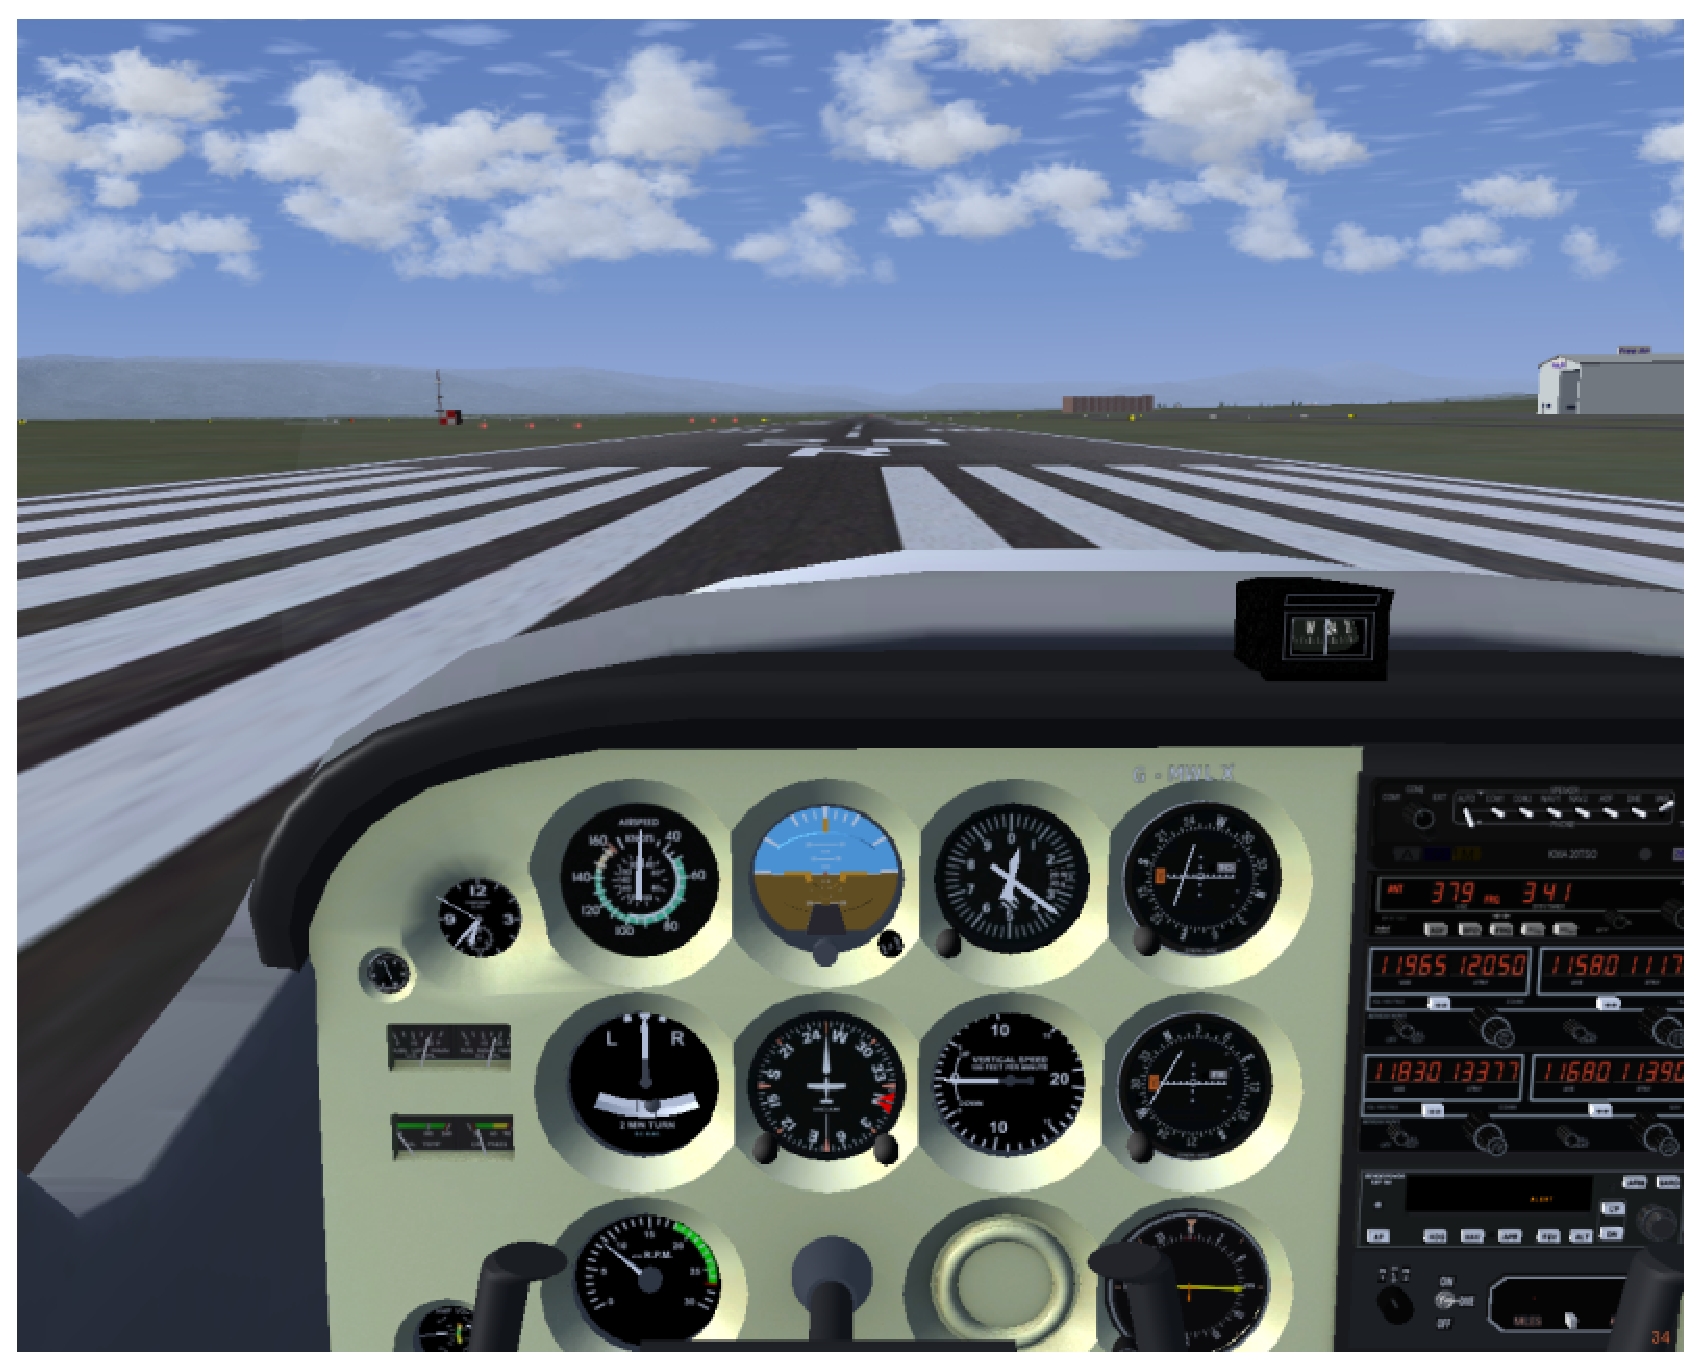
\includegraphics[clip,width=12.5cm]{panel3d}
}}

\smallskip
 \noindent
Fig.\,6: \textit{The 3D cockpit of the Cessna 172.}
\medskip

Aircraft within \FlightGear{} can have both a 2-dimensional instrument panel
and a 3-dimensional cockpit. The 3-dimensional cockpit provides a much
more realistic pilot-eye view, but can be difficult to read with small
monitors.

The default Cessna 172P (c172p) has both a 3-dimensional and 2-dimensional
cockpit. The 3-dimensional cockpit is activated by default when you start
\FlightGear{}, but you can overlay the 2-dimensional instrument panel by
selecting \texttt{View->Toggle 2D Panel} from the menu, or pressing the ``P'' key.

All panel levers and knobs can be operated with the mouse. To change a
control, just click with the left/middle mouse button on the
corresponding knob/lever. For controls that have a range of positions,
using the middle mouse button for larger adjustments. In general, clicking
on the right side of a control will increase the value, while clicking the left side
of the control will decrease the value.

Some instruments (particularly radios) also support use of a mouse scroll-wheel
to change values.

%%%%%%%%%%%%%%%%%%%%%%%%%%%%%%%%%%%%%%%%%%%%%%%%%%%%%%%%%%%%%%%%%%%%%%%%%%%%%%%%
%%%%%%%%%%%%%%%
\section{The Head Up Display\index{head up display}}
%%%%%%%%%%%%%%%%%%%%%%%%%%%%%%%%%%%%%%%%%%%%%%%%%%%%%%%%%%%%%%%%%%%%%%%%%%%%%%%%
%%%%%%%%%%%%%%%

\FlightGear{} also provides a \Index{HUD} (\textbf{H}ead \textbf{U}p
\textbf{D}isplay) \index{head up display}. HUDs are generally found in military
aircraft and some very advanced jets. However, \FlightGear{} also allows you
to use a HUD on many GA aircraft. To activat the HUD, press `h'.

The \Index{HUD} shown in Fig.\,7  displays all main flight parameters of the
plane. In the center you find the \Index{pitch indicator} (in degrees) with the
\Index{aileron indicator} above and the \Index{rudder indicator} below. A
corresponding scale for the elevator\index{elevation indicator} can be found
to the left of the pitch scale along with a pitch trim indicator. On the bottom
there is a simple \Index{turn indicator}.

There are two scales at the extreme left: The inner one displays the \Index{speed}
 (in kts) while the outer one indicates position of the \Index{throttle}.
The two scales on the extreme right display your \Index{height} - the left one
shows the height above ground while the right of it displays hieght above sea-level,
both being displayed in feet.

Besides this, the \Index{HUD} delivers some additions information. On the upper
left you will find date and time, along with your current position, in \Index{latitude}
and \Index{longitude}.

You can change color of the \textbf{HUD} using the ``H'' or ``'h''  key.
Pressing the toggle ``i/I'' minimizes/maximizes the HUD.

\medskip

 \centerline{\fbox{
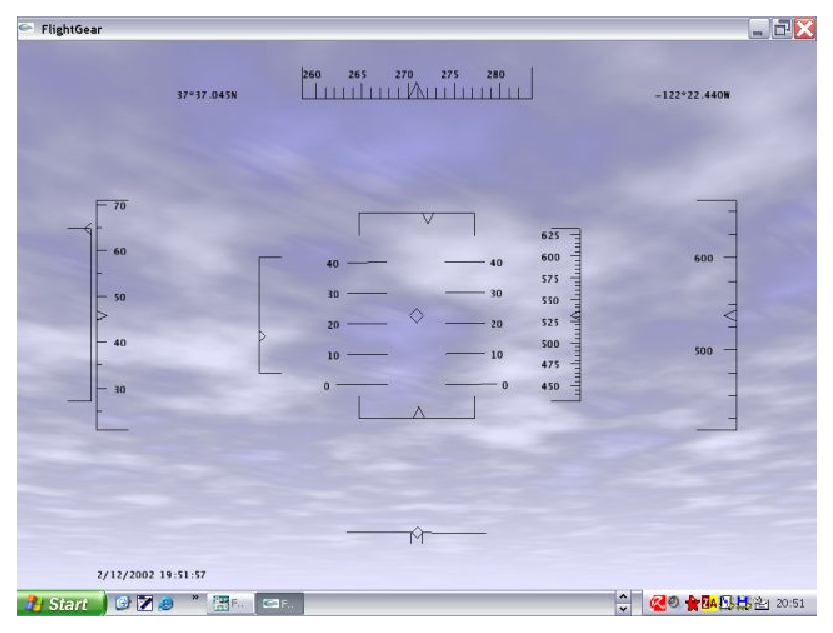
\includegraphics[clip,width=12.5cm]{hud2}
}}

\smallskip
 \noindent
Fig.\,7: \textit{The HUD, or Head Up Display.}
\medskip

%% Revision 0.00  1998/09/08  michael
%% Initial revision for version 0.53.
%% Revision 0.01  1998/09/20  michael
%% several extensions and corrections, added Fig.1.
%% revision 0.10  1998/10/01  michael
%% final proofreading for release
%% revision 0.11  1998/11/01  michael
%% Complete revision of keyborad controls, interesting places
%% revision 0.12  1999/03/07  michael
%% Corrected rudder key
%% revision 0.20  1999/06/04  michael
%% HUD completely rewritten, added panel section with picture, and menu section
%% updated keystrokes
%% revision 0.3 2000/04/20 michael
%% again updated and added keystrokes
%% revised menu entries
%% picture of new panel and re-written panel section
%% added mouse control section
%% Updated many keys, notably autopilot related, added two new tables
%% revision 0.4 2001/05/12 michael
%% updated/added many keystrikes, updated/added panel description
%% (radio stack etc.), new panel pic, panel before HUD now
%% short description of VOR/NDB
%% revision 0.41 2001/01/01 michael
%% added section on flight school material
%% added hints to user configurable *.xml files
%% revision 0.5 2002/01/01 michael
%% revised all changed keybindings now mostly read off of keyboard.xml
%% restructured tables more logically and put into separate files
%% for inclusion in Short Reference
%% New panel picture and revised descirption of panel according to new features
%% New HUD picture
%% revision 0.6 2002/09/05 michael
%% Several corrections/tweaks in plus renumbering of tables
%% Tweaks in menu entries
%% Added 3D cockpit picture
%% Changing numbers in radios
%% Added new menu items, swapped over 3D and 2-D pictures, as 3D cockpit is
%%  now the default
%% Revision 18/10/08: Numerous changes to improve readability, correct spelling errors etc.
%% Revision 8/3/09: Improved description of mouse modes.
%% Revision 26/12/09: Re-organization, move panel description to tutorial, update menu items.


%%
%% getstart.tex -- Flight Gear documentation: The FlightGear Manual
%% Chapter file
%%
%% Written by Michael Basler, started September 1998.
%%
%% Copyright (C) 2002 Michael Basler
%%
%%
%% This program is free software; you can redistribute it and/or
%% modify it under the terms of the GNU General Public License as
%% published by the Free Software Foundation; either version 2 of the
%% License, or (at your option) any later version.
%%
%% This program is distributed in the hope that it will be useful, but
%% WITHOUT ANY WARRANTY; without even the implied warranty of
%% MERCHANTABILITY or FITNESS FOR A PARTICULAR PURPOSE.  See the GNU
%% General Public License for more details.
%%
%% You should have received a copy of the GNU General Public License
%% along with this program; if not, write to the Free Software
%% Foundation, Inc., 675 Mass Ave, Cambridge, MA 02139, USA.
%%
%% $Id: features.tex,v 0.6 2002/09/09 Stuart
%% (Log is kept at end of this file)

%%%%%%%%%%%%%%%%%%%%%%%%%%%%%%%%%%%%%%%%%%%%%%%%%%%%%%%%%%%%%%%%%%%%%%%%%%%%%%%%%%%%%%%%%%%%%%%
\iflanguage{english}{
\chapter{Features}
\label{features}
}{}
\iflanguage{french}{
\chapter{Fonctionnalit\'{e}s}
\label{Fonctionnalit\'{e}s}
}{}
%%%%%%%%%%%%%%%%%%%%%%%%%%%%%%%%%%%%%%%%%%%%%%%%%%%%%%%%%%%%%%%%%%%%%%%%%%%%%%%%%%%%%%%%%%%%%%%
\iflanguage{english}{
\FlightGear{} contains many special features, some of which are not obvious to the new user. This section
describes how to enable and make use of some of the more advanced features.

Many of the features are under constant development, so the information here may not be completely up-to-date.
For the very latest information (and new features), see the \FlightGear{} Wiki, available from
\web{http://wiki.flightgear.org/}
}{}

\iflanguage{french}{
\FlightGear{} contient de nombreuses fonctonnalit\'{e}s sp\'{e}cifiques, certaines d'entre elles n'\'{e}tant pas
directement apparentes pour le nouvel utilisateur. Ce chapitre d\'{e}crit comment activer et utiliser quelques
unes des fonctionnalit\'{e}s les plus avanc\'{e}es.

De nombreuses fonctionnalit\'{e}s sont en d\'{e}veloppement permanent, donc l'information pr\'{e}sente dans le manuel
peut ne pas \^{e}tre compl\`{e}tement \`{a} jour.
For the very latest information (and new features), see the \FlightGear{} Wiki, available from
\web{http://wiki.flightgear.org/}
}{}

\iflanguage{english}{
\section{Multiplayer}\index{Multiplayer}\label{multiplayer}
}{}

\iflanguage{french}{
\section{Multijoueurs}\index{Multijoueurs}\label{multijoueurs}
}{}

\iflanguage{english}{
\FlightGear{} supports a multiplayer environment, allowing you to share the air with other flight-simmers.
For server details and to see who is online (and where they are flying), have a look at the excellent
multiplayer map, available from
}{}
\iflanguage{french}{
\FlightGear{} offre un environnement multijoueurs, vous permettant de partager l'air avec d'autres amateurs de simulation de vol.
Pour plus de d\'{e}tail sur les serveurs et pour voir qui est en ligne (et o\`{u} ils volent), allez jeter un \oe{}il \`{a} l'excellente
carte multijoueurs, disponible \`{a} l'adresse :
}{}

\noindent
\web{http://mpmap02.flightgear.org}

\iflanguage{english}{
Click on the `server' tab to see a list of multiplayer servers.
}{}
\iflanguage{french}{
Cliquez sur l'onglet `server' pour voir une liste des serveurs multijoueurs.
}{}

\iflanguage{english}{
\subsection{Quick Start}

You can connect to the MP environment from the MP Settings dialog under the Multiplayer menu. Simply select the
server closest to you from the list, enter a callsign (which will be seen by other players), and click
''Connect''.

To see a list of other pilots are in the area, select Pilot List from the Multiplayer menu.

All the standard MP servers are interconnected, so there is no need to be on the same server as people you are flying with.
}{}
\iflanguage{french}{
\subsection{D\'{e}marrage rapide}

Vous pouvez vous connecter \`{a} l'environnement multijoueurs (MP) \`{a} partir de la bo\^{i}te de dialogue du menu `Multijoueurs'. Choisissez simplement le
serveur le plus proche de chez vous \`{a} partir de la liste, entrez un indicatif (qui sera vu par les autres joueurs) et cliquez sur
''Connect''.

Pour affichez une liste des autres pilotes dans la zone, s\'{e}lectionnez Pilot List \`{a} partir du menu `Multijoueurs'.

Sous les serveurs multijoueurs standard sont interconnect\'{e}s, donc il n'est pas n\'{e}cessaire d'\^{e}tre connect\'{e} sur le
m\^{e}me serveur que les gens avec qui vous volez.
}{}

\subsection{Other Methods}

If you are connecting to a non-standard server, or the above method does not work, you can also connect
using the methods below.

\subsubsection{Using the FlightGear Launcher}

The final screen of the FlightGear Launcher has a section for Multiplayer.
Simply select the checkbox, enter the hostname and port
number you noted above and choose a callsign to identify yourself.
Your callsign can be up to 7 characters in length.
You must also check The AI models checkbox under Features to make other aircraft visible.

\subsubsection{Using the Command Line}

The basic arguments to pass to fgfs for multiplayer are these:

\begin{verbatim}
--multiplay=out,10,<server>,<portnumber>
--multiplay=in,10,<client>,<portnumber>
--callsign=<anything>
--enable-ai-models
\end{verbatim}

Where
\begin{enumerate}
\item <portnumber> is the port number of the server e.g. 5000.
\item <server> is the name of the multiplayer server e.g. mpserver01.flightgear.org.
\item <client> is the name of your computer, or the IP address ip address of the network interface being
used by FG to connect to the server - even if that's a local 192.168 type address. e.g. 192.168.0.1
\item <callsign> is the call sign to identify yourself, up to 7 characters, e.g. N-FGFS.
\end{enumerate}

Once the simulator has loaded, you should see yourself displayed on the map. If you don't, check the
console for error messages and see the Troubleshooting section below.

\subsection{Troubleshooting}

To get multiplayer to work, we need information about the IP address of our computer and the
ability to communicate with the server. How to get this information depends on your configuration and is described below.

\subsubsection{Those using a USB modem to connect to the Internet}

First of all, you need to know the IP address of the network interface you're going to be running FG multiplayer over.
If your Internet connection is via an ADSL modem that plugs directly into your computer with a USB connection, you
should be able to find your IP address by visiting http://www.whatismyip.com . Please note that this address may very well
change every now and again - if MP stops working, check this first.

\subsubsection{Those using some kind of Ethernet router to connect to the Internet}

Otherwise, your connection is likely via some kind of router that connects to your computer via an RJ-45, or "Ethernet" connector
(similar shape to most Western telephone plugs), or by a wireless link. You need to find the IP address of that network interface.

Under Linux, this can be found by logging in as root and typing "ifconfig". You may find more than one interface listed,
beginning with "lo" - ignore that one. You should have something like "eth0" or "wlan0" also listed - look through this block
of text for "inet addr". This will be followed directly by the number you're looking for, e.g. "inet addr:192.168.0.150"

Under Windows XP, click start, run, and type "cmd". In the terminal window which appears, type "ipconfig"
This should show you your IP address - note it down.

With Windows 98, click start, run, and type "winipcfg" to get information about your IP address.

\subsubsection{If It Still Doesn't Work}

You MUST give your local, behind-the-router IP address for MultiPlayer to work. Trust me on this one!

You should check that your firewall is not causing problems - either turn it off temporarily or add an exception
to allow incoming connections on port 5000.

If it's still just not working for you, ask nicely on the FlightGear IRC channel and someone should be able to assist.

\section{Aircraft Carrier}\index{Aircraft Carrier}\label{carrier}

\FlightGear{} supports carrier operations on the Nimitz, (located near San Fransisco), Vinson, San Antonio, Foch, and Eisenhower.
The carriers are equipped with working catapult, arrester wires, elevators, TACAN and FLOLS.

To enable the carrier, you must edit your preferences.xml file in \$FG\_ROOT using a text editor (e.g. Notepad
under Windows). Search for the word ``nimitz''. You ought to find something that looks like this;

\begin{verbatim}
<!--<scenario>nimitz_demo</scenario>-->
\end{verbatim}

You should remove the ``comment'' marks so that it looks like this;


\begin{verbatim}
<scenario>nimitz_demo</scenario>
\end{verbatim}

Also ensure that the line above that referring to ai being enabled is set to "true"

Save the file and quit the text editor.

\subsection{Starting on the Carrier}

You are now ready to start FlightGear. To position your aircraft on the carrier at startup,
use the following command line options:

\begin{verbatim}
--carrier=Nimitz --aircraft=seahawk
\end{verbatim}

Please note the uppercase ``N' in ``Nimitz'.

If you are using the Windows or OS X launcher to run FG, you should find a text entry box in the gui that
allows you to specify command line options, add the above options there.

Note that several FG aircraft are carrier capable, but the seahawk is possibly the easiest to fly to begin with.

\subsection{Launching from the Catapult}

Once FlightGear has started, you should ensure that the parking brakes are off and press and hold ``L'' to
engage the launchbar. You must hold down ``L'' until the launch bar has engaged.
You should notice the aircraft being pulled into alignment with the catapult and see
the strops appear and hold down the aircraft.  This will only happen if your aircraft is
close enough to the correct spot on the catapult; as a rough guide, for the default
parking position the seahawk's nose should be rougly level with the deck observation bubble.

To get the carrier into as good a position as possible for launch, select the ``ATC/AI'' menu, then
check the ``Turn into wind'' box under the ``AI Carrier'' section. You should now notice the carrier
begin to pick up speed and turn into the wind, and naturally the deck may tilt somewhat as it turns.
You should wait for this maneuver to finish and the deck to return to level before moving on to the next stage.

Being attached to the catapult, you should spool up the engines to full power, ensure the brakes are off
and that all flight controls are in a suitable position for launch (stick held right back with the seahawk.)
When ready, press ``C'' to release the catapult. Your aircraft will be hurled forward off the deck, and
you should be able to raise the undercarriage and climb slowly away, being careful to avoid stalling.

\subsection{Finding the Carrier - TACAN}

Actually finding the carrier in a vast expanse of open water can be very difficult, especially if visibility
is poor. To assist with this task, Nimitz is equipped with TACAN, which allows a suitably-equipped
aircraft (including the Seahawk) to obtain a range and bearing to the carrier. First, you must set
the appropriate TACAN channel, 029Y in this case, in the radios dialogue (ctrl-r or choose
Equipment/Radio Settings from the FG menubar). You should, if within range, notice the DME instrument
show your distance from the carrier, and the ADF instrument (next to the DME in the seahawk) should
indicate a bearing to the carrier. Turn to the indicated heading and you should see the DME dial
indicate your closing in on the carrier.

\subsection{Landing on the Carrier}

This is the most difficult part of the operation, as in real life. You might well find Andy Ross' tutorial on
operating the A4 Skyhawk useful. It is available from here:

\noindent
\web{http://wiki.flightgear.org/A-4F\_Skyhawk\_Operations\_Manual}

Once you have used the TACAN to locate the carrier, you must
line up with the rear of the flight deck. As this part of the deck is at an angle to the course of the vessel,
you may need to correct your alignment often. Ensure that the aircraft is in the correct configuration for
approach (the Help/Aircraft Help menu should contain useful data for your aircraft) and that the gear and
the arrestor hook are down.

As you approach you should see, on the left hand side of the deck, a set of brightly coloured lights - called
the Fresnel Lens Optical landing System (FLOLS). This indicates your position on the landing glideslope.
You will see a horizontal row of green lights, and when approximately on the glideslope, an orange light
(known in some circles as the ``meatball'') approximately in line with the green lights. When approaching
correctly, the meatball appears in line with the green lights. If you are high it is above, and when low
it is below. If you are very low the meatball turns red. If you fly to keep the meatball aligned you
should catch number 3 wire.

Carrier landings are often described as ``controlled crashes'' and you shouldn't waste your time attempting
to flare and place the aircraft gently on the deck like you would with a conventional landing - ensuring that
you catch the wires is the main thing.

Immediately your wheels touch the deck, you should open the throttles to full power, in case you have
missed the wires and need to ``go around'' again; the wires will hold the aircraft if you have caught them,
even at full power.

If you wish, you can then raise the elevators from the ATC/AI menu, taxi onto one of the elevators,
lower it (uncheck the box on the menu) and taxi off into the hangar.

Don't be discouraged if you don't succeed at first - it's not an easy maneouver to master. If after a little
practice you find the Seahawk too easy, you could move on to the Seafire for more of a challenge!


\section{Atlas\label{Atlas}}\index{Atlas}

Atlas is a "moving map" application for FlightGear. It displays the aircraft in relation to the terrain below,
along with airports, navigation aids and radio frequencies.

Further details can be found on the Atlas website:

\noindent
\web{http://atlas.sourceforge.net}

\section{Multiple Displays}\index{Multiple Displays}

\FlightGear{} supports multiple displays. Using some straightforward
 XML, you can configure multiple "slave cameras" that are offset from
the main view, so you can use multiple monitors to display a
single view of the simulator. For example, you can have one display
showing the view straight ahead, while two additional displays show
the view to either side.

Information on configuring multiple displays can be found in the
README.multiscreen file in the docs directory of your \FlightGear{}
installation.

\section{Multiple Computer}\index{Multiple Displays}

\FlightGear{} allows you to connect multiple instances of the program
using the very flexible I/O subsystem, and display completely different views
 and controls on different computers. This can be used in combination
 with the Multiple Display support to create a more sophisticated environment
 with separate cockpit panel displays and even a separate control
station allowing an instructor to fail instruments, change the weather etc.

An example of this is the 747 cockpit project.

\noindent
\web{http://www.flightgear.org/Projects/747-JW/}

\subsection{Setup}

Each instance of \FlightGear{} can support a single display. Due to the
complexity of the FDM and graphics, \FlightGear{} is very processor-intensive,
so running multiple instances of \FlightGear{} on a single machine is not
recommended.

You will therefore need a computer for each view of the simulation you wish
to display, including the panel. The computers obviously must be networked
and for simplicity should be on the same subnet.

One computer is designated as the master. This computer will run the FDM and
be connected to controls such as yokes, joysticks and pedals. As the machine is
running the FDM, it usually only displays a simple view, typically the main
panel, to maximize performance.

All other computers are designated as slaves. They are purely used for display
purposes and receive FDM information from the master.

\subsection{Basic Configuration}

Creating a basic configuration for multiple displays is straightforward. The
master computer needs to broadcast the FDM and control information to the slaves.
This is done using the following command line options:

\begin{verbatim}
--native-fdm=socket,out,60,,5505,udp
--native-ctrls=socket,out,60,,5506,udp
\end{verbatim}

The slave computers need to listen for the information, and also need to have
their own FDMs switched off:

\begin{verbatim}
--native-fdm=socket,in,60,,5505,udp
--native-ctrls=socket,in,60,,5506,udp
--fdm=null
\end{verbatim}

\subsection{Advanced Configuration}

The options listed above will simply show the same view on both machines. You will probably also want to set the
following command-line options on both master and slave computers.

\begin{verbatim}
--enable-game-mode  (full screen for glut systems)
--enable-full-screen (full screen for sdl or windows)
--prop:/sim/menubar/visibility=false (hide menu bar)
--prop:/sim/ai/enabled=false (disable AI ATC)
--prop:/sim/ai-traffic/enabled=false (disable AI planes)
--prop:/sim/rendering/bump-mapping=false
\end{verbatim}

If using the master computer to display a panel only, you may wish to create a full-screen panel for the
aircraft you wish to fly (one is already available for the Cessna 172), and use the following options.

\begin{verbatim}
--prop:/sim/rendering/draw-otw=false (only render the panel)
--enable-panel
\end{verbatim}

\section{Recording and Playback}\index{Playback}

As well as the Instant Replay feature within the simulator, you can record your
flight for later analysis or replay using the I/O system.  Technical details of
how to record specific FDM information can be found in the
\$FG\_ROOT/protocol/README.protocol file.

To record a flight, use the following command line options:

\begin{verbatim}
--generic=file,out,20,flight.out,playback
\end{verbatim}

This will record the FDM state at 20Hz (20 times per second), using the playback
protocol and write it to a file flight.out.

To play it back later, use the following command line options:

\begin{verbatim}
--generic=file,in,20,flight.out,playback
--fdm=external
\end{verbatim}

The playback.xml protocol file does not include information such as plane type,
time of day, so you should use the same set of command line options as you
did when recording.

\section{Text to Speech with Festival}\index{Text To Speech}

\FlightGear{} supports Text To Speech (TTS) for ATC and tutorial messages through the festival TTS
engine (\web{http://www.cstr.ed.ac.uk/projects/festival/}). This is available on many Linux distros,
and can also be installed easily on a Cygwin Windows system. At time of writing, support on other platforms is unknown.

\subsection{Installing the Festival system}

\begin{enumerate}
\item Install festival from \web{http://www.cstr.ed.ac.uk/projects/festival/}

\item Check if Festival works. Festival provides a direct console interface. Only the relevant lines are
shown here. Note the parentheses!

\begin{verbatim}
$ festival
festival> (SayText "FlightGear")
festival> (quit)
\end{verbatim}

\item Check if MBROLA is installed, or download it from here:

\web{http://tcts.fpms.ac.be/synthesis/mbrola/}

See under "Downloads"m "MBROLA binary and voices"
(link at the bottom; hard to find). Choose the binary for your platform. Unfortunately, there's no
source code available. If you don't like that, then you can skip the whole MBROLA setup.
But then you can't use the more realistic voices. See below for details of more voices.
Run MBROLA and marvel at the help screen. That's just to check if it's in the path and executable.

\begin{verbatim}
$ mbrola -h
\end{verbatim}
\end{enumerate}

\subsection{Running FlightGear with Voice Support}

First start the festival server:

\begin{verbatim}
$ festival --server
\end{verbatim}

Now, start \FlightGear{} with voice support enabled. This is set through the
/sim/sound/voices/enabled property. You can do this through the command line as follows.

\begin{verbatim}
$ fgfs --aircraft=j3cub \
       --airport=KSQL \
       --prop:/sim/sound/voices/enabled=true
\end{verbatim}

Of course, you can put this option into your personal configuration file.
This doesn't mean that you then always have to use FlightGear together with Festival.
You'll just get a few error messages in the terminal window, but that's it. You cannot enable
the voice subsystem when FlightGear is running.

To test it is all working, contact the KSFO ATC using the ' key. You should hear "your"
voice first (and see the text in yellow color on top of the screen), then you should hear
ATC answer with a different voice (and see it in light-green color).

ou can edit the voice parameters in the preferences.xml file, and select different screen colors
and voice assignments in \$FG\_ROOT/Nasal/voice.nas. The messages aren't written to the
respective /sim/sound/voices/voice[*]/text properties directly, but rather to aliases
/sim/sound/voices/{atc,approach,ground,pilot,ai-plane}.

\subsection{Troubleshooting}

On some Linux distros, festival access is restricted, and you will get message like the following.

\begin{verbatim}
client(1) Tue Feb 21 13:29:46 2006 : \
  rejected from localhost.localdomain
not in access list
\end{verbatim}

Details on this can be found from:

\web{http://www.cstr.ed.ac.uk/projects/festival/manual/festival\_28.html\#SEC130}.

You can disable access restrictions from localhost and localhost.localdomain by adding
the following to a .festivalrc file in \$HOME:
\begin{verbatim}
(set! server_access_list '("localhost"))
(set! server_access_list '("localhost.localdomain"))
\end{verbatim}

Or, you can just disable the access list altogether:

\begin{verbatim}
(set! server_access_list nil)
\end{verbatim}

This will allow connections from anywhere, but should be OK if your machine is behind a
firewall.

\subsection{Installing more voices}

I'm afraid this is a bit tedious. You can skip it if you are happy with the default voice.
First find the Festival data directory. All Festival data goes to a common file tree,
like in FlightGear. This can be /usr/local/share/festival/ on Unices. We'll call that
directory \$FESTIVAL for now.

\begin{enumerate}
\item Check which voices are available. You can test them by prepending "voice\_":

\begin{verbatim}
$ festival
festival> (print (mapcar (lambda (pair) (car pair)) \
                                    voice-locations))
(kal_diphone rab_diphone don_diphone us1_mbrola \
                   us2_mbrola us3_mbrola en1_mbrola)
nil
festival> (voice_us3_mbrola)
festival> (SayText "I've got a nice voice.")
festival> (quit)
\end{verbatim}

\item Festival voices and MBROLA wrappers can be downloaded here:

\web{http://festvox.org/packed/festival/1.95/}

The "don\_diphone" voice isn't the best,
but it's comparatively small and well suited for "ai-planes". If you install it,
it should end up as directory \$FESTIVAL/voices/english/don\_diphone/.
You also need to install "festlex\_OALD.tar.gz" for it as \$FESTIVAL/dicts/oald/ and
run the Makefile in this directory. (You may have to add "--heap 10000000" to the
festival command arguments in the Makefile.)

\item Quite good voices are "us2\_mbrola", "us3\_mbrola", and "en1\_mbrola". For these you need to
install MBROLA (see above) as well as these wrappers: festvox\_us2.tar.gz, festvox\_us3.tar.gz,
and festvox\_en1.tar.gz. They create directories \$FESTIVAL/voices/english/us2\_mbrola/ etc.
The voice data, however, has to be downloaded separately from another site:

\item MBROLA voices can be downloaded from the MBROLA download page (see above).
You want the voices labeled "us2" and "us3". Unpack them in the directories that
the wrappers have created: \$FESTIVAL/voices/english/us2\_mbrola/ and likewise for "us3" and "en1".

\end{enumerate}

\section{Air-Air Refuelling}\label{aar}
  \index{Air-Air Refuelling}

As the name suggests, Air-Air Refueling (AAR) involves refueling an aircraft
(typically a short-range jet fighter) from a tanker aircraft by flying in close
formation. There are two types of refueling system supported. The KC135-E tanker
has a boom that connects to a receiver on the refueling aircraft. The smaller
KA6-D deploys a hose, into which the refueling aircraft inserts a probe.

A number of aircraft support AAR, including the T-38, Lightning, A-4F, Vulcan,
Victor (which can also act as a tanker) and A-6E. You can tell if a particular
aircraft support AAR by looking at the AI/ATC menu. If the ``Tanker'' menu item
is enabled, the aircraft support AAR.

\subsection{Setup}

To set up AAR, simply start FlightGear with an AAR-enabled aircraft, take-off
and climb to 15,000ft. Once cruising at this altitude, select AI/ATC->Tanker,
and select ``Request'', which will spawn a new tanker in clear air at
approximately your altitude.

FlightGear will report the altitude, speed, and TACAN identifier of the tanker.
Program your TACAN with the TACAN identifier reported by the tanker (from the
Equipment->Radio Settings dialog, or your cockpit controls). Depending on your
aircraft, the tanker may also appear on your radar. If you require more help to
find the tanker, you can select ``Get Position'' to be told the tanker
location relative to yourself

Turn to an appropriate heading, guided by the TACAN bearing (you should
try a "leading" approach to close in on the tanker) and look for the
tanker on the radar or nav. screen.  Around 5nm away, you should reduce
your speed to around 20kts faster than the tanker - a "slow overtake".  The
KC135 will be visible from about 10nm, the KA6-D, being smaller, just over 1 nm.
If you find yourself overshootng, deploy your airbrakes.

Close to within 50ft of the tanker (don't get too close, or you may collide with
the tanker itself).  You should see indication in
the cockpit that you are receiving fuel - there is a green light in the
A4 fuel gauge, and you should see the indicated tank load increase.

Once your tanks are full, or you have taken as much fuel as you wish,
close the throttle a little, back away from the tanker and continue
your intended flight.

Successfully refueling is not easy and can take a lot of practise, as in real
life. Here are some helpful hints for making contact.

\begin{enumerate}
\item Approach the tanker slowly. It is very easy to overshoot and be unable to
spot where the tanker has gone.
\item If you are having difficulty matching the speed of the tanker due to the
throttle being too sensitive, try deploying your airbrakes. This will require
more power to achieve the same speed and will reduce the throttle sensitivity.
\item To reduce your workload, you may be able to use the autpilot to stay at
the correct altitude and/or speed. This is technically cheating, though NASA
recently demonstrated that an advanced autopilot can perform AAR without pilot
intervention.
\item Bear in mind that as you receive fuel your aircraft will become heavier
and the center of gravity will move, affecting the trim of the aircraft.
\item The tanker aircraft fly a clock-wise "race-track" pattern in the sky.
While it is possible to stay connected during these turns, you may find it
easier to wait until the tanker has settled on its new course before refueling.
The tanker aircraft provide warnings when they are intending to turn.
\end{enumerate}

\subsection{Multiplayer Refueling}

Refuelling is possible within a Multiplayer session using the KC135 or Victor.
The pilot of this aircraft should use the callsign "MOBIL1", "MOBIL2" or "MOBIL3".
Other numbers are acceptable, but only these three have A-A TACAN
channels assigned.  These are 060X, 061X and 062X respectively.

If the receiving aircraft uses a YASim FDM, there are no further
complications.  Should the receiving aircraft be JSBSim based, the user
must make sure that there are no AI tankers in their configuration.
This means disabling (commenting out) all refuelling "scenarios" in the
relevant aircraft-set.xml and in preferences.xml.

MP refuelling works in exactly the same way as AI refuelling and is a
fun challenge.  It is best to ensure that your network connection is as
free from interruptions as possible; the MP code does a degree of
prediction if there is a "blip" in the stream of packets and this can
make close formation flight very difficult or even impossible.

%% Revision 1.00  2009/11/15  Stuart. Updates for v1.9.2
%% Revision 0.00  2006/01/01  Stuart
%% Initial revision for version 0.9.9.

\part{Tutorials}
%%
%% tutorials.tex -- Flight Gear documentation: The FlightGear Manual
%% Chapter file
%%
%% Written by Michael Basler, started September 1998.
%%
%% Copyright (C) 2002 Michael Basler
%%
%%
%% This program is free software; you can redistribute it and/or
%% modify it under the terms of the GNU General Public License as
%% published by the Free Software Foundation; either version 2 of the
%% License, or (at your option) any later version.
%%
%% This program is distributed in the hope that it will be useful, but
%% WITHOUT ANY WARRANTY; without even the implied warranty of
%% MERCHANTABILITY or FITNESS FOR A PARTICULAR PURPOSE.  See the GNU
%% General Public License for more details.
%%
%% You should have received a copy of the GNU General Public License
%% along with this program; if not, write to the Free Software
%% Foundation, Inc., 675 Mass Ave, Cambridge, MA 02139, USA.
%%
%% $Id: flight.tex,v 0.5 0.6 2002/09/09 michael
%% (Log is kept at end of this file)

%%%%%%%%%%%%%%%%%%%%%%%%%%%%%%%%%%%%%%%%%%%%%%%%%%%%%%%%%%%%%%%%%%%%%%%%%%%%%%%%%%%%%%%%%%%%%%%
\chapter{Tutorials}
\label{tutorials}
%%%%%%%%%%%%%%%%%%%%%%%%%%%%%%%%%%%%%%%%%%%%%%%%%%%%%%%%%%%%%%%%%%%%%%%%%%%%%%%%%%%%%%%%%%%%%%%

If you are new to flying, an advanced simulator such as \FlightGear{} can seem
daunting: You are presented with a cockpit of an aircraft with little 
information on how to fly it.

In real life, when learning to fly you would have an instructor sitting next to
you to teach you how to fly and keep you safe.

While we cannot provide a personal instructor for every virtual pilot, there are
a number of tutorials available that you can follow to become a proficient
virtual pilot.

\section{In-flight Tutorials}

\FlightGear{} contains an in-flight tutorial system, where a simulated 
instructor provides a virtual `lesson'. These vary between aircraft from
 simple tutorials teaching you how to start the engines on the aircraft,
to full lessons teaching you how to fly for the first time.
To access tutorials, Select Start Tutorial from the Help menu. 

The tutorial system works particularly well with the Festival TTS system 
(described above).

For simplicity, run tutorials with AI aircraft turned off from
the Options item on the AI/ATC menu. Otherwise, ATC messages 
may make it difficult to hear your instructor.

Each tutorial consists of a number of discrete steps which you must complete.
Your instructor will provide directions on how to complete each step, and
observer how you perform them, providing additional guidance if required.

Within a tutorial, to ask your instructor to repeat any instructions, press 
`+'. You can pause the tutorial at any time using the `p' key. To stop the 
tutorial select Stop Tutorial from the Help menu. 

\subsection{Cessna 172P tutorials}

If this is your first time flying, a number of tutorials exist for the
Cessna 172P designed to teach you the basics of flight, in a similar way to a
real flight school. The tutorials are based around Half-Moon Bay (KHAF) and
Livermore Municipal (KLVK) airports near San Francisco. Both these airports are
provided in the base package. To start the tutorials, select the Cessna 172P
aircraft, and a starting airport of KHAF or KLVK, using the wizard, or the
command line:

\begin{verbatim}
$ fgfs --aircraft=c172p --airport=KHAF
\end{verbatim}

When the simulator has loaded, select Start Tutorial from the Help menu. You
will then be presented with a list of the tutorials available. Select a tutorial
and press Next. A description of the tutorial is displayed. Press Start
 to start the tutorial.

\section{FlightGear Tutorials}

The following chapters provide \FlightGear{} specific tutorials
to take the budding aviator from their first time in an aircraft to flying in 
the clouds, relying on their instruments for navigation. If you have never flown
a small aircraft before, following the tutorials provides an excellent 
introduction to flight.

Outside of this manual, there is an excellent tutorial written by David
Megginson \index{Megginson, David} -- being one of the main developers
of \FlightGear{} -- on flying a basic airport circuit specifically
using \FlightGear{}. This document includes a lot of screen shots,
numerical material etc., and is available from

\medskip
\web{http://www.flightgear.org/Docs/Tutorials/circuit}.
\medskip

\section{Other Tutorials}

There are many non-\FlightGear{} specific \Index{tutorial}s, many of which are 
applicable. First, a quite comprehensive manual of this type is the 
\Index{Aeronautical Information Manual}, published by the \Index{FAA}, 
and available at

\medskip
\web{http://www.faa.gov/ATPubs/AIM/}.
\medskip
\noindent

This is the Official Guide to Basic Flight Information and ATC Procedures by 
the FAA. It contains a lot of information on flight rules, flight safety, 
navigation, and more. If you find this a bit too hard work, you may prefer 
the \Index{FAA Training Book},

\medskip
\web{http://avstop.com/AC/FlightTraingHandbook/},
\medskip
\noindent

which covers all aspects of flight, beginning with the theory of flight and the
working of airplanes, via procedures like takeoff and landing up to emergency 
situations. This is an ideal reading for those who want to learn some basics on 
flight but don't (yet) want to spend bucks on getting a costly paper pilot's 
handbook.

While the handbook mentioned above is an excellent introduction on \Index{VFR} 
(Visual Flight Rules), it does not include flying according to \Index{IFR} 
(Instrument Flight Rules). However, an excellent introduction into navigation 
and flight according to Instrument Flight Rules written by Charles Wood
\index{Wood, Charles} can be found at

\web{http://www.navfltsm.addr.com/}.

Another comprehensive but yet readable text is John Denker's\index{Denker, John}
''\Index{See how it flies}'', available at
\medskip

\web{http://www.monmouth.com/~jsd/how/htm/title.html}.
\medskip

 \noindent
This is a real online text book, beginning with Bernoulli's principle, drag and
power, and the like, with the later chapters covering even advanced aspects of 
VFR as well as IFR flying

%% Revision 0.00  1998/09/08  michael
%% Initial revision for version 0.53.
%% Revision 0.01  1998/09/20  michael
%% several extensions and corrections, added Fig.1.
%% revision 0.10  1998/10/01  michael
%% final proofreading for release
%% revision 0.11  1998/11/01  michael
%% Complete revision of keyborad controls, interesting places
%% revision 0.12  1999/03/07  michael
%% Corrected rudder key
%% revision 0.20  1999/06/04  michael
%% HUD completely rewritten, added panel section with picture, and menu section
%% updated keystrokes
%% revision 0.3 2000/04/20 michael
%% again updated and added keystrokes
%% revised menu entries
%% picture of new panel and re-written panel section
%% added mouse control section
%% Updated many keys, notably autopilot related, added two new tables
%% revision 0.4 2001/05/12 michael
%% updated/added many keystrikes, updated/added panel description
%% (radio stack etc.), new panel pic, panel before HUD now
%% short description of VOR/NDB
%% revision 0.41 2001/01/01 michael
%% added section on flight school material
%% added hints to user configurable *.xml files
%% revision 0.5 2002/01/01 michael
%% revised all changed keybindings now mostly read off of keyboard.xml
%% restructured tables more logically and put into separate files 
%% for inclusion in Short Reference
%% New panel picture and revised descirption of panel according to new features
%% New HUD picture
%% revision 0.6 2002/09/05 michael
%% Several corrections/tweaks in plus renumbering of tables
%% Tweaks in menu entries
%% Added 3D cockpit picture
%% Changing numbers in radios
%% revision 0.7 2005/10/29 Stuart Buchanan
%% Re-ordering for inclusion of Cross Country tutorial

\definecolor{green}{cmyk}{0,0.25,0.5,0}
\definecolor{orange}{cmyk}{0,0.25,0.5,0}
\newcommand{\weblong}[2]{\href{#1}{#2}} % definition of long hyperreferences
\newcommand {\key}[1]{\textbf{\ttfamily{#1}}} % definition of key
\newcommand {\button}[1]{\textbf{\sffamily{#1}}} % definition of GUI button
\newcommand {\command}[1]{{\ttfamily{#1}}} % definition of console command
\newcommand {\excl}[1]{
	\begin{tabular}{r p{0.75\textwidth}}
	\hspace*{5mm}\LARGE{\textcolor{green}{$!$
	%\ArrowBoldDownRight
}} & #1\\		
\end{tabular}
}
\newcommand {\photo}[3]
{\begin{center}
  \includegraphics[width=0.5\textwidth]{img/#3}
\end{center}}		

\newcommand {\fg}{\FlightGear}

%%%%%%%%%%%%%%%%%%%%%%%%%%%%%%%%%%%%%%%%%%%%%%%%%%%%%%%%%%%%%%%%%%%%
\chapter{A Basic Flight Simulator Tutorial\label{basic}}
%%%%%%%%%%%%%%%%%%%%%%%%%%%%%%%%%%%%%%%%%%%%%%%%%%%%%%%%%%%%%%%%%%%%

\section{Foreword}
\label{sec:Foreword}
    
Aviation is about extremes:

\begin{itemize}
	\item An airplane is quite fragile and flies at high speeds. 
  Yet it is one of the safest forms of transport.
	\item Pilots must constantly follow rules and procedures. 
  Yet an airplane is a symbol of freedom.
	\item With a little training, flight a small aircraft is easy.
  Yet if a problem occurs, you must be able to resolve it in a  few seconds.
	\item Many flight tutorials are written with a lot of humor.
  Yet not taking flying seriously will bring you down to earth prematurely.
\end{itemize}
    
The aircraft used in this tutorial is the
\weblong{http://en.wikipedia.org/wiki/Cessna_172} {Cessna 172p}, the standard
aircraft in many real life flight schools and a great airplane:


\begin{center}
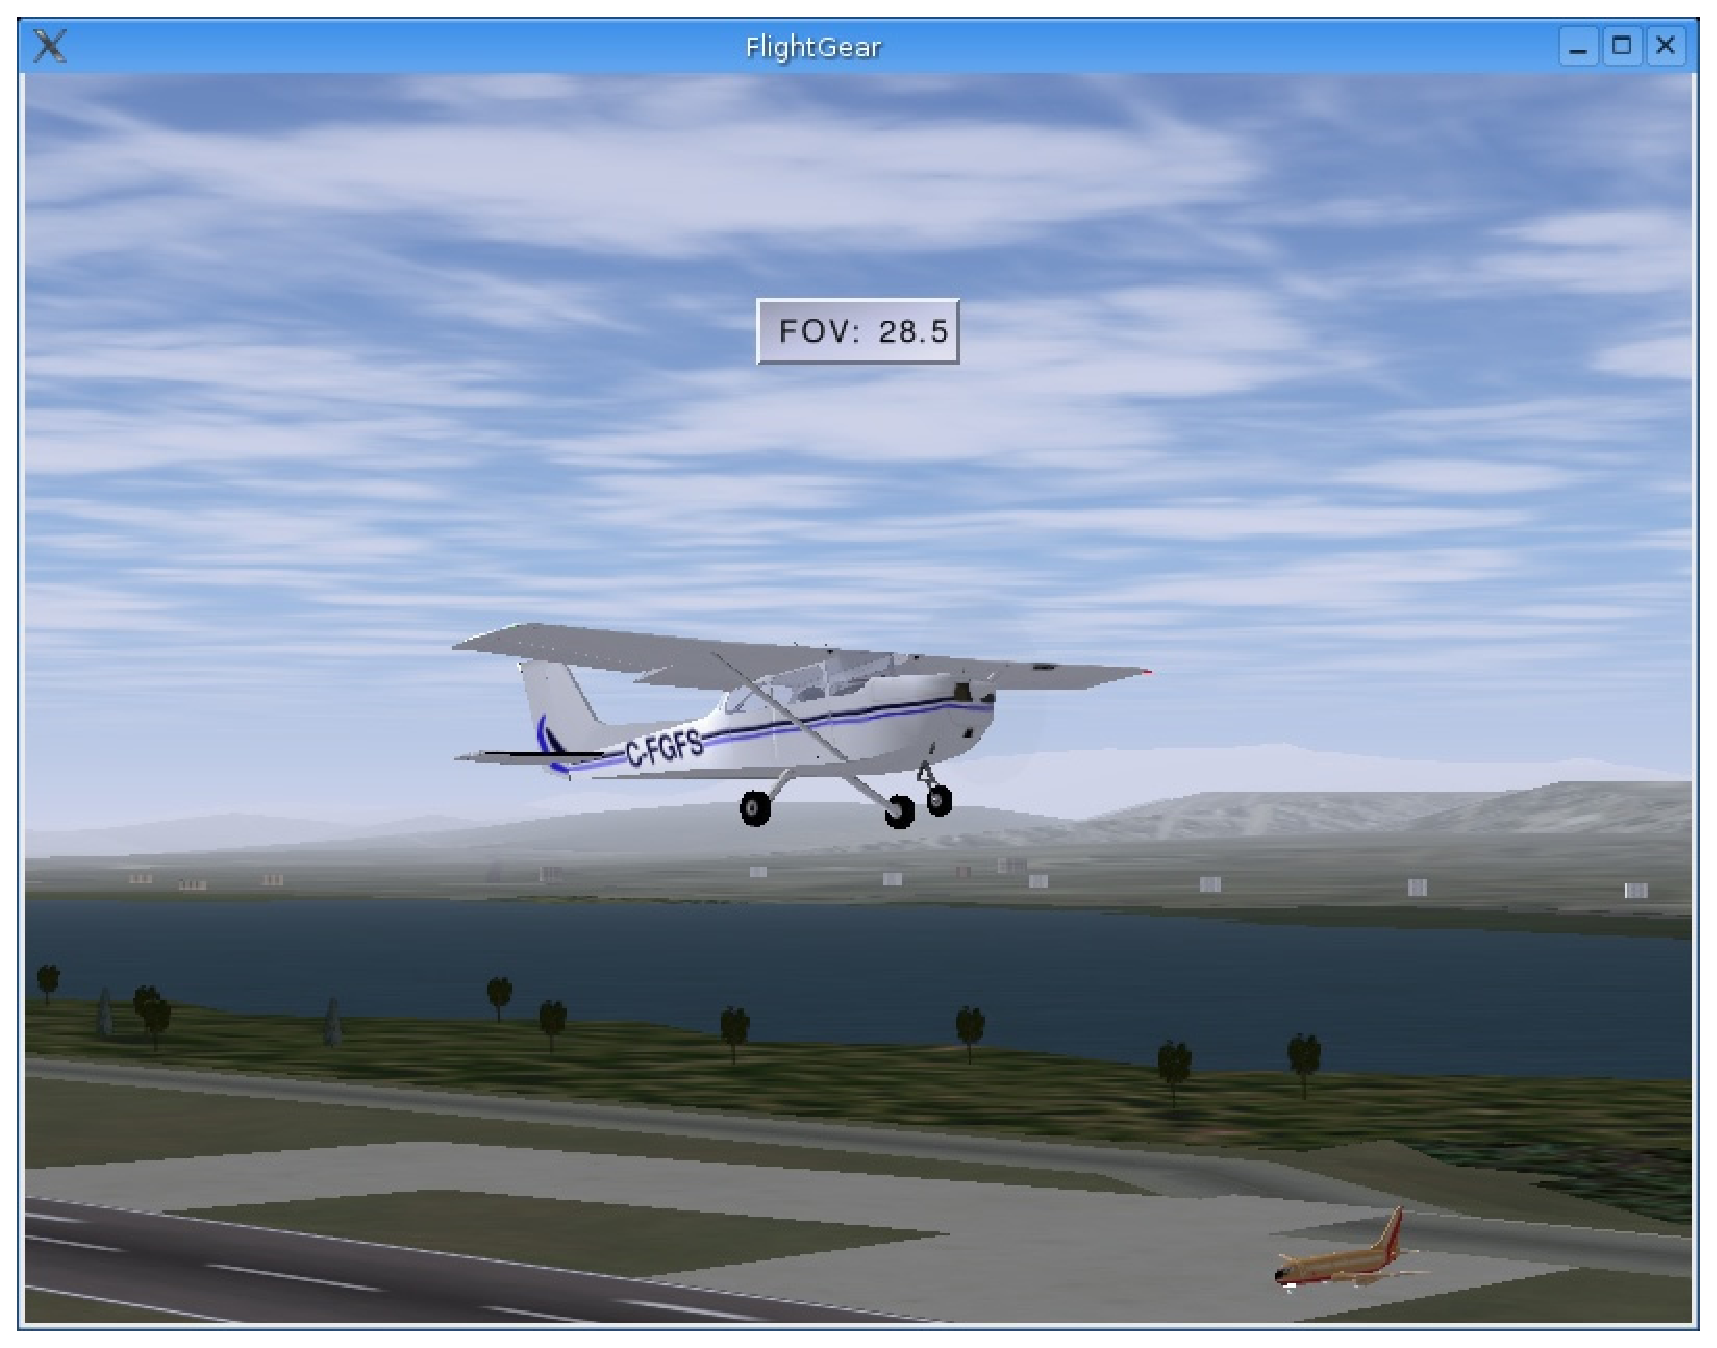
\includegraphics[width=0.5\textwidth]{img/tut_1}
\end{center}
    
You may find the following articles useful if read in conjunction with this
tutorial. They contain many answers to questions that
may arise while reading this tutorial. This first one in paricular is a good
intruction to the airplane's main parts and controls:
\begin{itemize}
	\item \weblong{http://www.gleim.com/aviation/ltf/howtheyfly.php?PHPSESSID=889ab9792636f430a66e3e5d70f7d346}    {http://www.gleim.com/aviation/ltf/howtheyfly.php?PHPSESSID=889ab9792\\636f430a66e3e5d70f7d346}
	\item \weblong{http://www.pilotfriend.com/flight_training/new_site/aerodynamics/aircraft\%20controls.htm}    {http://www.pilotfriend.com/flight\_training/new\_site/aerodynamics/\\aircraft\%20controls.htm}
	\item \web{http://www.flightgear.org/Docs/getstart/getstart.html}
	\item \web{http://en.wikipedia.org/wiki/Aircraft}
	\item \web{http://en.wikipedia.org/wiki/Flight\_controls}
	\item \web{http://en.wikipedia.org/wiki/Airplane\_flight\_mechanics}
	\item \web{http://en.wikipedia.org/wiki/Aircraft\_engine\_controls}
	\item \web{http://www.firstflight.com/flt1.html}
	\item \weblong{http://www.avsim.com/mike/mickey_site/ppilot/ppilot_faq/pp_cessnas.html}{http://www.avsim.com/mike/mickey\_site/ppilot/\\ppilot\_faq/pp\_cessnas.html}
	\item \web{http://www.ig-wilson.com/index.php?f16land}
	\item \web{http://www.navfltsm.addr.com/}
\end{itemize}

This tutorial is accurate to the best of my knowledge, but inevitably will
contain some mistakes. I apologize in advance for any bad habits you may
develop from following this tutorial.
\section{Starting Up}
\label{sec:Hardware}
    
     
On MS Windows, \fg{} has a GUI Wizard that will let you choose what
to fly and where to fly from. First choose the Cessna 172p airplane as shown 
below. To match this tutorial do not choose the 2D panel version. 
(You may however find in the future that the 2D version is more appropriate 
for training) Press the \button{Next} button to choose your airport.


\begin{center}
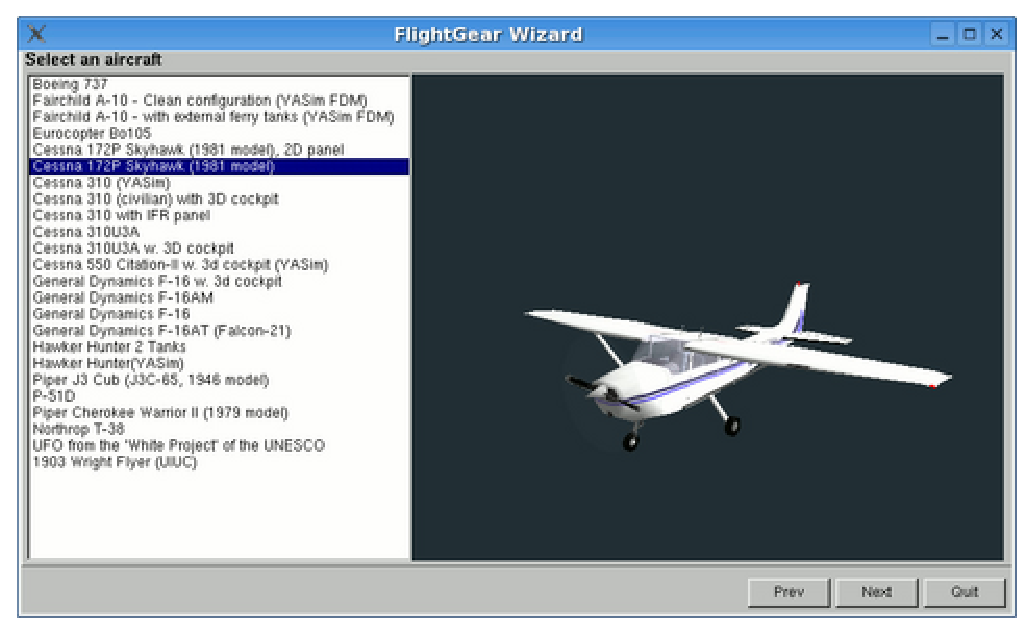
\includegraphics[width=0.5\textwidth]{img/tut_2}
\end{center}
    
You can start from any airport for this tutorial, but I will assume that you 
will start from FlightGear's default airport of San Francisco (KSFO):


\begin{center}
\includegraphics[width=0.5\textwidth]{img/tut_3}
\end{center}

Once you have selected KSFO and pressed the \button{Next} button, you can set
any number of options for the simulator. For your first flight, I suggest
starting at noon. I woul dalso recommend that you start with a small resolution
of $800\times600$. Later on you can play around with the options and use a
higher resolution, but this obviously adversly affects performance.Press the 
\button{Run} button and the \fg{} will start with the options you selected.


\begin{center}
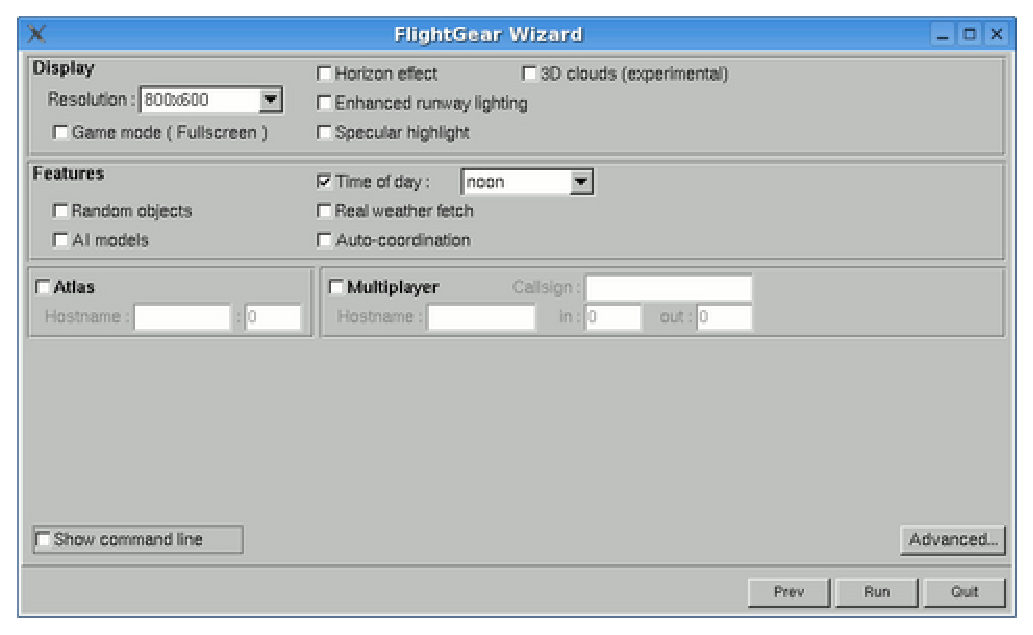
\includegraphics[width=0.5\textwidth]{img/tut_4}
\end{center}

   If you have problems running the latest version FlightGear on
   your Windows system, you may want to try an earlier version with lower
   graphics requirements (for example 0.9.8) You can find previous releases on 
   the FTP mirrors mentioned at the top of the \fg{} download page:
   \weblong{http://www.flightgear.org/Downloads/binary.shtml}.
   
If you are running under Windows Me and the flight simulator suddenly starts
\index{troubles!stuttered simulation}stuttering, with the frame rate dropping, 
try killing all tasks except Explorer and Systray before you
launch FlightGear. If one of the tasks you kill is an antivirus or
such protection software, this is an obvious security risk. Also, on one
Windows Me machine, a \fg{} of $800\times600$ yielded good results,
while a lower resolution of $640\times480$ triggered much lower FPS levels 
(Frames Per Second).)

On Linux and other Unix-like 
systems, you may have to run \fg{} from the command line. If you have
installed \fg{} but cannot find it within your menu system, try the following:

\begin{itemize}
  \item From a terminal window (also named ``console'' window) try
  running the  \command{fgrun} command. If installed, this will run the same 
  cute dialog windows as under Windows.

	\item Alternatively, open a terminal window and type the following command:
  \command{fgfs --timeofday=noon}. If the FlightGear window you get is too 
  small, close it and restart FlightGear with this command: 
  \command{fgfs --timeofday=noon --geometry=1024x768}.
\end{itemize}

Without the \command{--timeofday=noon} option, \fg{} will start at the current
time in San Francisco - often night-time if you are in Europe. To get a 
daytime environment from within the simulator, 
select \button{Weather->Time of Day} from the menu and select \button{Noon}.


\begin{center}
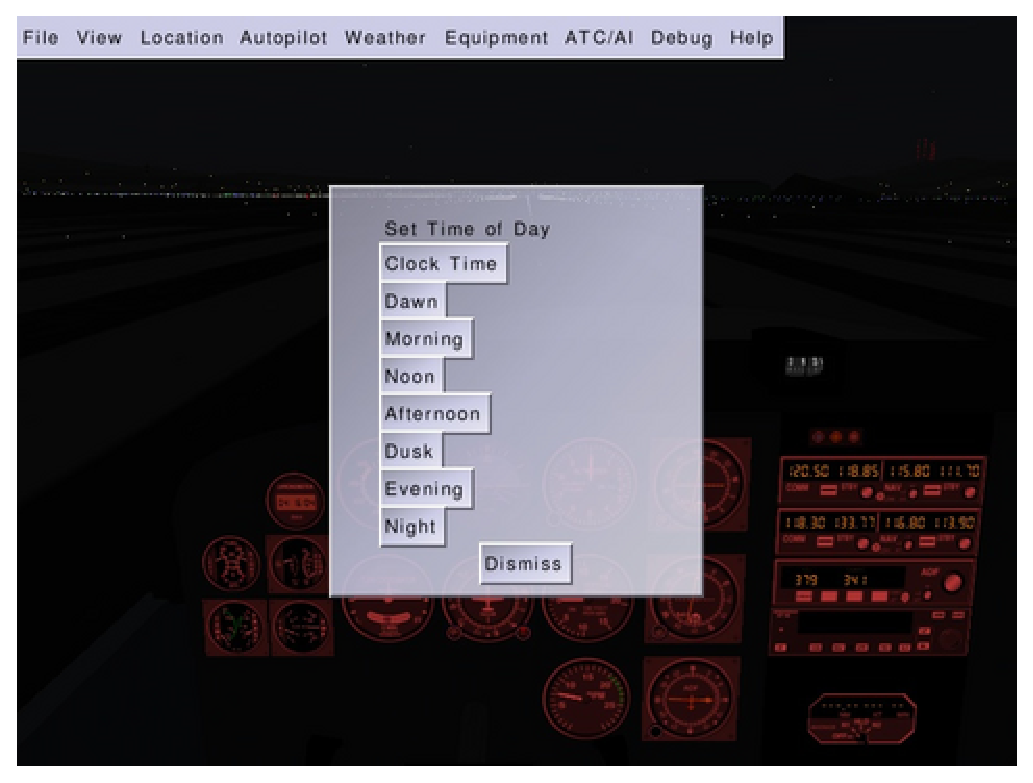
\includegraphics[width=0.5\textwidth]{img/tut_5}
\end{center}


If running \fg{} from a men (e.g. under KDE or Gnome), you can edit the 
FlightGear launch icon properties and change the simple \command{fgfs} fgfs 
command to something like \command{fgfs --timeofday=noon --geometry=1024x768},
or include whatever command options you wish. Further details of the command
line options can be found in Chapter~\ref{takeoff}, 
\textit{Takeoff: How to start the program}.

\section{The First Challenge - Flying Straight}
\label{sec:FlyingStraight}
    
Once \fg{} is started you will see the following window and hear the sound of 
an engine:


\begin{center}
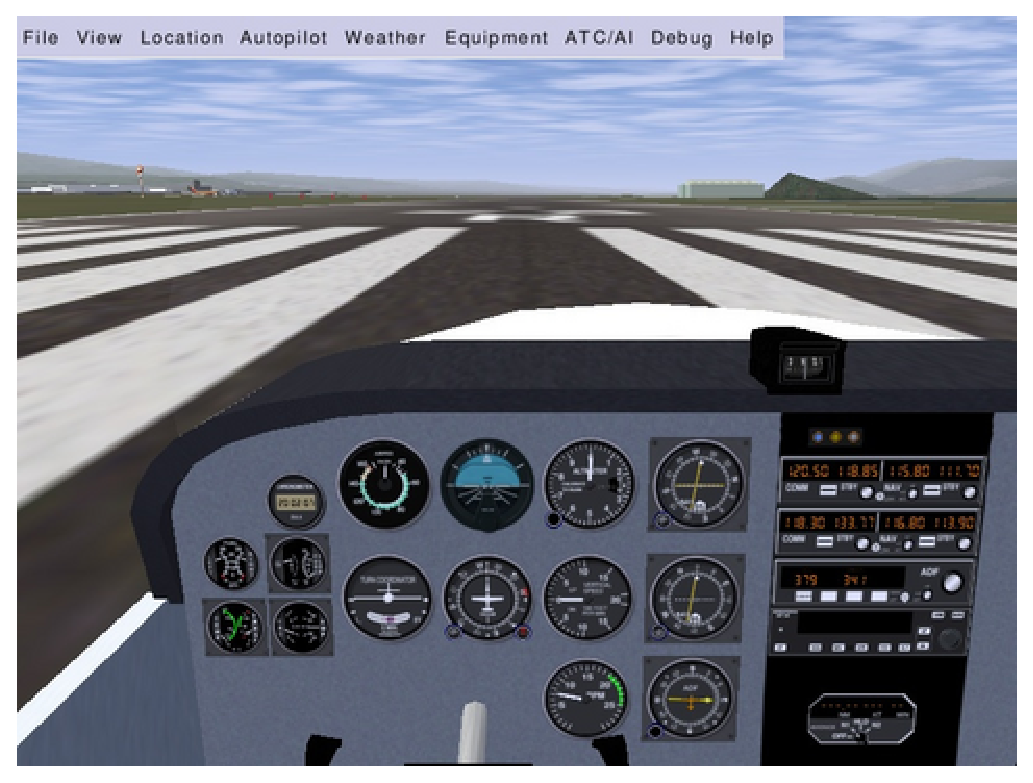
\includegraphics[width=0.5\textwidth]{img/tut_6}
\end{center}

On startup, the aircraft is at the end of the runway with the engine running at
low power. The airplane will ocassionally tremble a little, but it won't move.
    
\subsection*{About the keyboard.}\index{keyboard}
    
\begin{itemize}
	\item In this tutorial, a lowercase key letter indicates you should simply
  press that key. An uppercase means you must press shift and that key. 
  (The \textcolor{blue}{\key{$\Uparrow$~Shift}} keys are those two keys with 
  a hollow fat arrow pointing upwards.) In other words: if you are told to type
  ``v'', simply hit the \key{v} key briefly. 
  \index{keyboard!uppercase and lowercase keys} If you are told to type ``V'', 
  press the \key{Shift} key down and while you have it pushed down, hit the 
  \key{v} key, then release the \key{Shift}  key. (In short: V is the same as 
  \key{Shift-v}.)
	\item The tutorial will assume you have the the \key{NumLock} switched on. 
  \index{keyboard!numeric} When switched on, you should find a small green
  light on at the right of your keyboard. Press the 
  \textcolor{green}{\key{NumLock}}key repeatedly until the lamp is on.
\end{itemize}


\begin{center}
\includegraphics[width=0.5\textwidth]{img/tut_7}
\end{center}

\key{v}\index{view!changing}
Press \key{v}, to view the aircraft from the outside. Type v repeatedly to
scroll through a number of different views until you return to the cockpit.
Typing \key{V} will cycle backwards through the views.):


\begin{center}
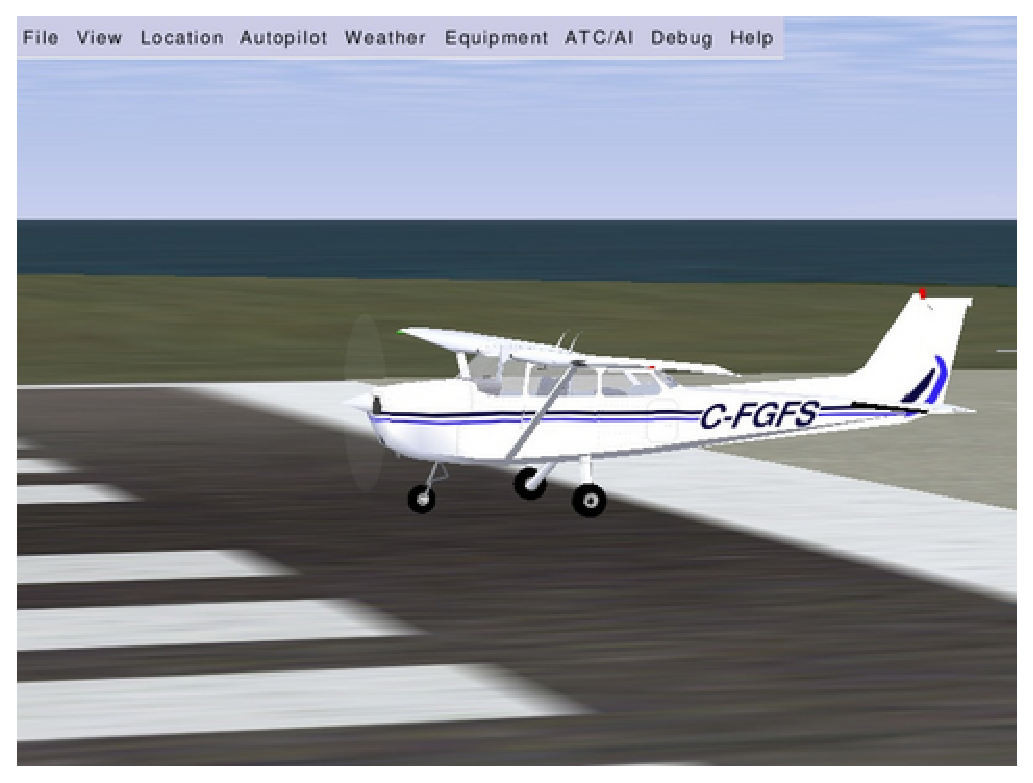
\includegraphics[width=0.5\textwidth]{img/tut_8}
\end{center}

In real life, we would have inspected the airplane all around to check 
everything is working, nothing is hampering the moving parts, 
and nothing is obstructing the instrument openings. In the simulator, this is
already done for us before we start.

Hold the \key{Page Up} key down for eight or so lengthy seconds. You will
hear the engine sound rise.

The airplane will start accelerating down the runway. As it does so, it will 
drift to the left, before finally taking off, banking to the left, 
falling to the ground and crashing. 

\index{view!instant replay}
You can see a replay of the crash using the  \button{View -> Instant Replay}
menu. Click the \button{Replay} button at the bottom of the dialog window, then
use \key{v} and \key{V} to see the airplane from the outside. The
picture below shows the end part of the flight. You can take a snapshot by
typing the \key{F3} key. You can alos use the \key{F10} key to toggle the menu 
bar on or off.


\begin{center}
\includegraphics[width=0.5\textwidth]{img/tut_9}
\end{center}

Having observed your crash, exit from \fg (using \button{File->Quit}) 
and restart the simulator using the same options as before.

In order to fly straight you need the airplane's control\index{yoke}
\weblong{http://en.wikipedia.org/wiki/Yoke_(aircraft)}{yoke}:


\begin{center}
\includegraphics[width=0.5\textwidth]{img/tut_10}
\end{center}

You can control the yoke using a joystick, or by moving the mouse. For this 
you need to be in mouse yoke mode. Get in that mode by clicking the right 
mouse button. The mouse cursor becomes a $+$ sign. Move the mouse and see the 
yoke moving accordingly. Type \key{v} to see the plane from the outside. If you
move the mouse again you will see the tail
\weblong{http://en.wikipedia.org/wiki/Elevator_(aircraft)}{elevator}
and the \weblong{http://en.wikipedia.org/wiki/Aileron}{ailerons}
at both wings ends. If your viewpoint is too far from the aircraft to see the
movement, type \key{x} a few times to zoom in. 
Type \key{X} to zoom back out. \key{Ctrl-x} for default zoom. Type
\key{V} to get back inside the plane.

Clicking the right mouse button again gets you in mouse view mode.
In this mode the mouse cursor will be a $\leftrightarrow$. sign. This allows you
to look around easily. Clicking the left mouse button will re-center the view. 
A further right click will return you to the normal mouse mode.

To summarize, the right mouse button cycles the mouse through three modes:
\begin{itemize}
	\item \textit{Normal mode}\index{mouse!normal mode}. This mode allows you to 
  click on the menu and on the instrument panel.
	\item \textit{Yoke mode}\index{mouse!yoke mode}.\index{yoke!mouse yoke mode} 
  The mouse controls the yoke (+ pointer shape). 
	\item \textit{View mode}\index{mouse!view mode}. The mouse controls the 
  direction you look towards  $\leftrightarrow$) pointer shape).
\end{itemize}

Try taking off again using the mouse to control the yoke. Right-click to put 
the mouse in yoke mode ($+$pointer shape) and raise the engine throttle to 
maximum by holding the \key{Page Up} key down. Do not try to keep the airplane 
rolling straight on the runway using the mouse/yoke. Let it drift leftwards.
Wait till it rises in the air. Then use the mouse to try and get the
airplane to fly straight. (If you want to control the airplane on the
ground see section \ref{sec:TaxiTurning}.)

You will find that you must prevent the airplane from banking to the left:


\begin{center}
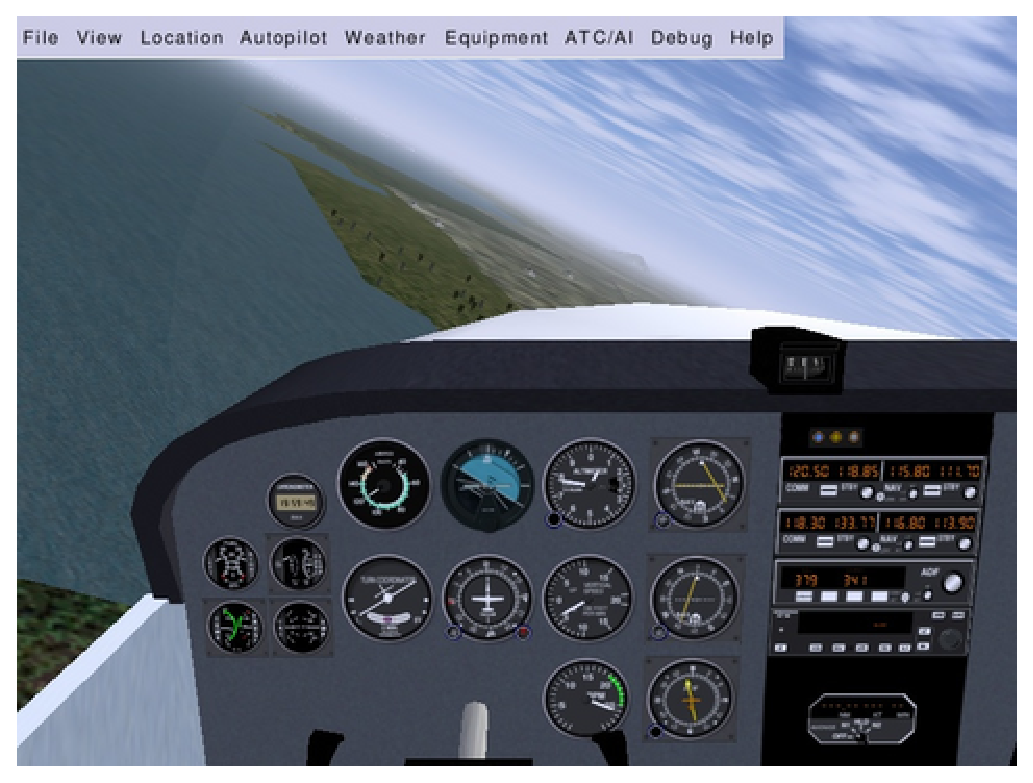
\includegraphics[width=0.5\textwidth]{img/tut_11}
\end{center}

%\pagebreak[4]

Prevent it from banking to the right:


\begin{center}
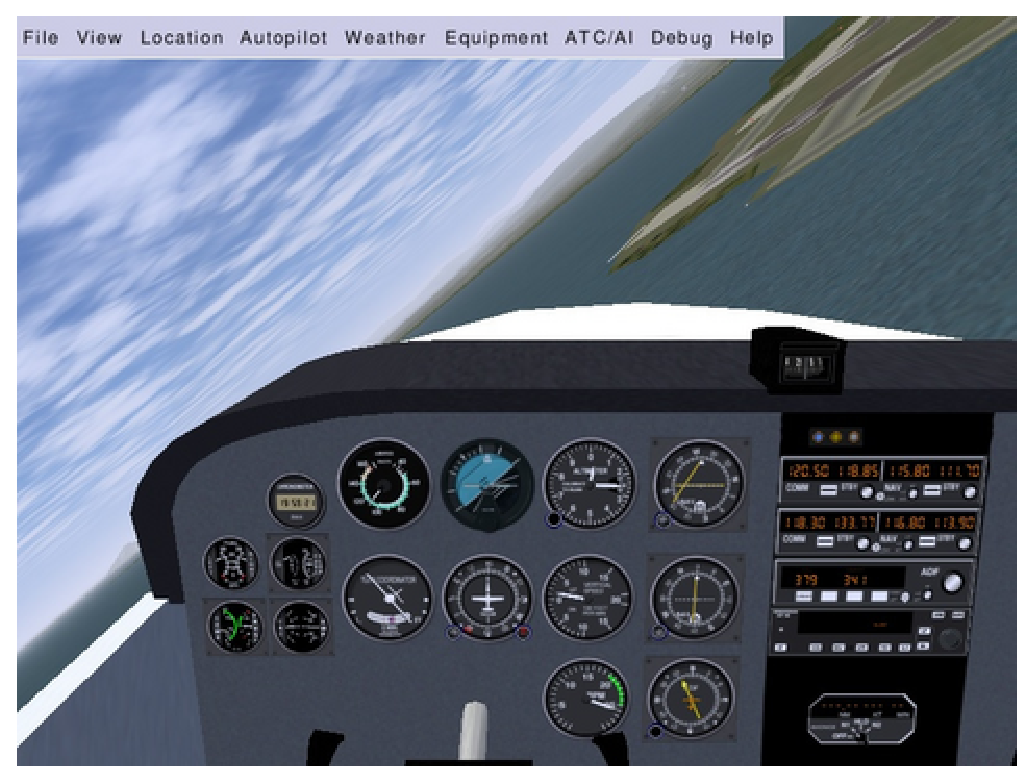
\includegraphics[width=0.5\textwidth]{img/tut_12}
\end{center}

Prevent it from plunging to the ground:


\begin{center}
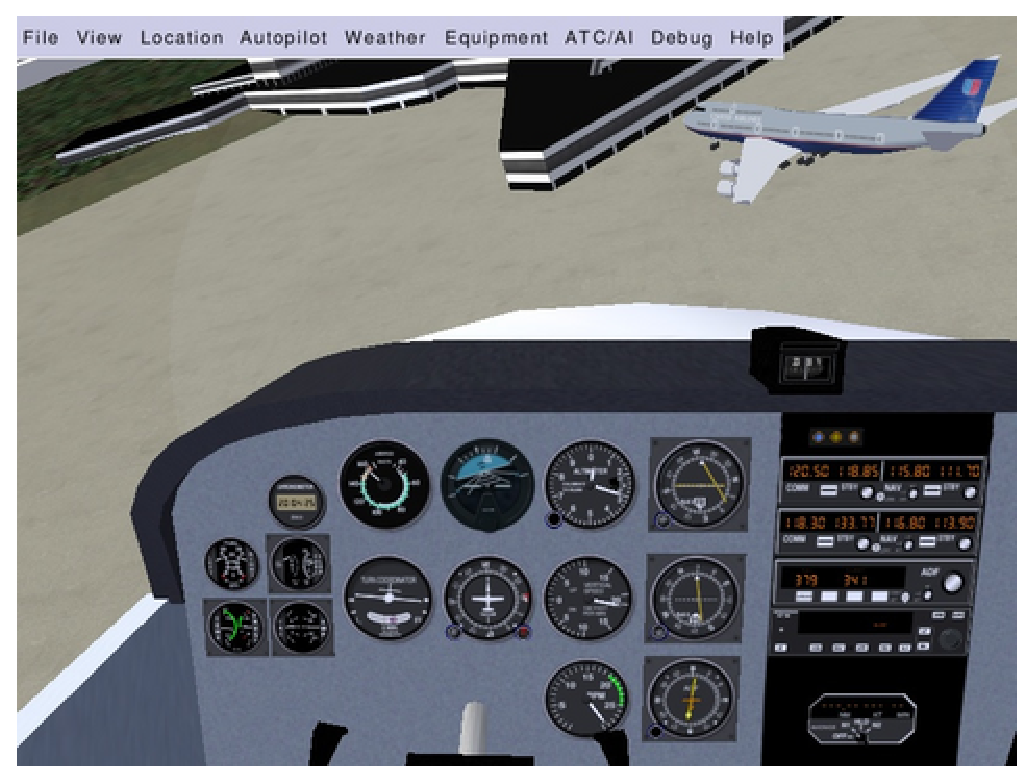
\includegraphics[width=0.5\textwidth]{img/tut_13}
\end{center}

%\pagebreak[4]

Try to fly more or less straight, with the horizon stable above the airplane 
nose:


\begin{center}
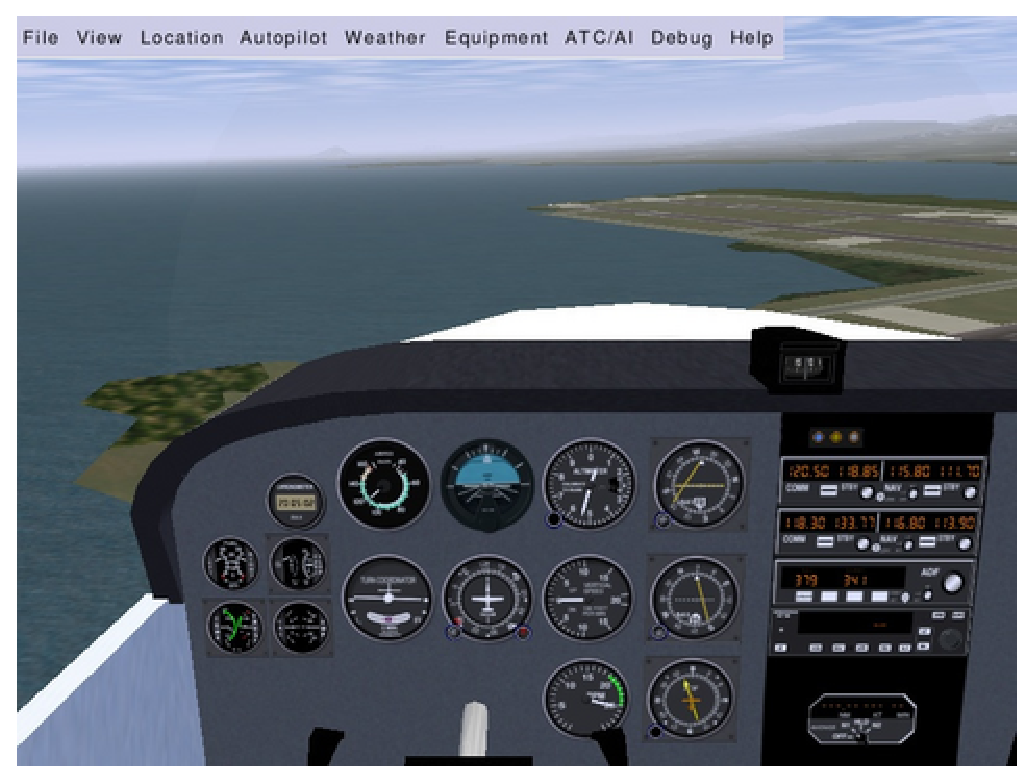
\includegraphics[width=0.5\textwidth]{img/tut_15}
\end{center}

Whatever your skills at video games or simpler simulators, you will probably 
not succeed. The airplane will crash, probably quite soon after take-off.
This is the moment where most candidates get desperate and abandon trying 
to fly a simulator or a real aircraft. Just hold tight and keep trying. 
Eventually you will develop a feel for the control inputs required.

\index{yoke!pulling}
The most common error is moving the mouse forwards to bring the nose up. In
fact, you must pull the yoke by moving the mouse backwards to do this. 

Equally, when you want to lower the airplane's nose, you must move
the mouse forwards. This can seem odd, but all airplane control yokes
are designed that way. With time, you will wonder how you every thought it
worked any other way. \index{troubles!mouse speed} You will also find that 
small mouse movements have a large effect on the aircraft. You may find that
decreasing your mouse sensitivity may help initially.

If you have difficulty visualising this, the following analogy may help.
Imagine a soccer ball is on your desk and you have ``glued'' your hand 
to the top of it. If you move your hand forwards the ball will roll forwards 
and your fingers will point to to the desk. If you move your hand backwards the 
ball will roll  back and your fingers will now point up at the ceiling. 
Your hand is the airplane:


\begin{center}
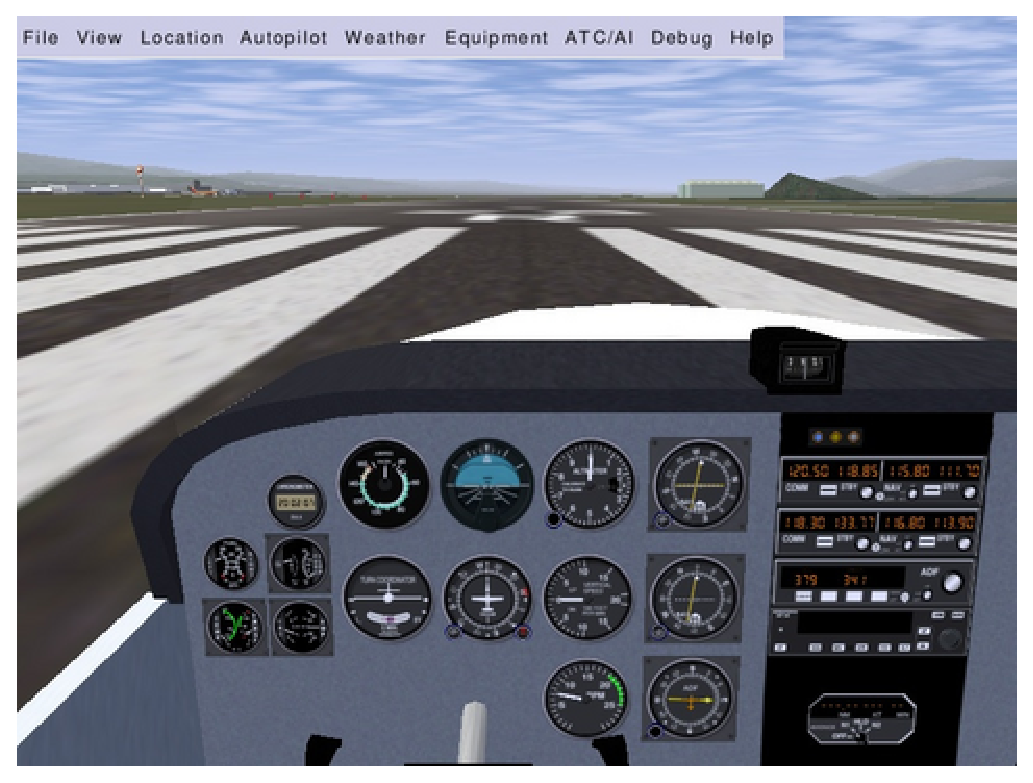
\includegraphics[width=0.5\textwidth]{img/tut_6}
\end{center}

Another common error is the assumption that the control inputs directly
match airplane bank. In other words, you believe if the control yoke is
level, the airplane will fly level. This is false. Actually the yoke
bank controls the speed at which the airplane banks. If the airplane is
banked 20$\textdegree$ to the left and the control yoke is level, the
airplane will stay banked at 20$\textdegree$ left until some other force
affects it. If you want to return the airplane to level flight, you have to
turn the control yoke slightly to the right (move the mouse slightly
rightwards) and keep it slightly to the right for a while. The airplane
will turn slowly rightwards. Once it is level with the horizon, bring the
control yoke level too. Then the airplane will stay level (until some other
force changes its orientation).

A third error is trying to find ``the right position'' for the
yoke/mouse. Naturally, you will want to find the fine tuning that will leave 
the airplane fly straight. Actually there is no such ideal yoke
position. The airplane is inherintely unstable in the air. You must constantly 
correct the airplane's attitude and keep it flying straight with tiny movements
of the mouse. This may seem to take all your concentration intially,
but just like driving a car, keeping the aircraft straight and level will
become second nature. You can also use the to keep the airplane level
during long flights.

A key helper in making the small adjustments is to keep your eyes on the outside
scenery and not get fixated on the instruments or the yoke. Check the angle of 
the horizon and its height above the airplane's nose. The horizon line and the
airplane engine cover are your main flight instruments. Look at
the instrument panel only once in a while.

While the mouse is in yoke\index{yoke!mouse yoke mode} control mode
($+$ pointer shape), don't move it close to the FlightGear window
edges. Once the mouse leaves the window, it stops controlling the aircraft.
If you want to get the mouse outside of the window, first go back to standard 
mouse mode by clicking two times on the right mouse button.

You can also control the yoke using the four \key{keyboard arrow} keys
or the keypad \key{8}, \key{2}, \key{4} and \key{6} keys. While initially this
may seem easier than the mouse, you cannot make the very fine adjustments
required for accurate flying.

You may hear beeping sounds while flying around the airport. Those are
landing aid signals\index{landing!aid signals}. Don't worry about them for the
moment - they aren't warning your of danger.

You will know that you have mastered this when you can make the aircraft climb
steadily in the air. The next step is to learn to keep the aircraft at a constant
altitude, or to make it ascend or descend slowly and under your control.

Keeping the aircraft at a constant altitude involves observing the altimeter
and making small changes with the mouse forwards or backwards to stop the 
aircraft ascending or descending respectively.

\index{altimeter} The altimeter instrument is at the middle top of the 
instrument panel. The long needle shows hundreds of feet, the short needle 
shows thousands of feet. The altimeter below shows an altitude of
300 feet, approximately 100 meters.


\begin{center}
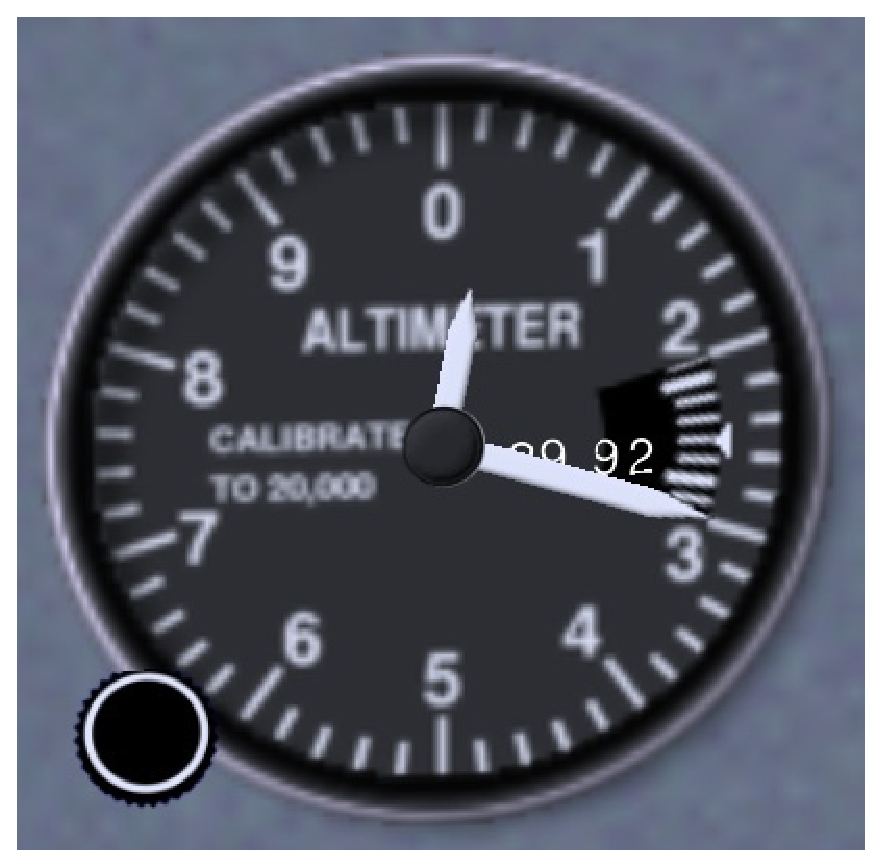
\includegraphics[width=0.25\textwidth]{img/tut_17}
\end{center}

As you ascend or descend the altimeter will change accordingly, turning 
anti-clockwise as you descend, and clockwise as you gain height. If you see
the altimeter ``unwinding'' you will be able to tell that you are losing height
and move the mouse backwards slightly to raise the nose.
After a while you will notice that when flying level the nose of the aircraft
is always in the same position relative to the horizon. This is the aircraft
attitude for level flight. By putting the nose in that same position, you will
achieve almost level flight without having to reference the instruments. From
there you can fine-tune your altitude.

Beware: an altimeter does not automatically show the absolute altitude
above sea level\index{altitude!absolute}. You must adjust for the local air
pressive. The little black knob on the lower left side of the
altimeter\index{altimeter!tuning} allows you to adjust the altimeter. Start 
\fg{} and stay on the ground. Click (in normal mouse mode) inside the black knob. 
A click on the left half makes the altimeter turn back. On the right half the 
altimeter turns forward. Use that little knob to tune in the curraent altitude. 
The principle is you use the knob when you are sure about the altitude. If
you know you are at 1,100 feet altitude, tune in 1,100 feet on the
altimeter. Clicking with the middle mouse button makes the knob
turn faster. Type \key{Ctrl}-\key{c} to see the two button halves
highlighted.

To make settings the altimeter easier, airports advertise their altitude in 
various ways. They may provide a radio service (called ATIS in the USA) 
to broadcast the current air pressure at sea level. This is expressed in 
inches of mercury. The altimeter contains a small scale inside which is
calibrated in this way. You can set your altimeter using this scale. 
Alternatively, if you are on the ground and know the altitude of the airport,
you can simply adjust your altimeter until it displays the correct altitude.

\vfill


\begin{center}
\includegraphics[width=0.25\textwidth]{img/tut_18}
\end{center}

Note that there is an important difference between ``altitude above sea 
level'' and ``altitude above the ground''. If you fly near Mount Everest at an
altitude of 24,000 feet above sea level (AMSL), your altitude above the ground 
(AGL) will be much less. Knowing the altitude of the ground around you is 
obviously useful.

    \section{Basic Turns}
    \label{sec:InFlightTurning}

Once you are able to fly straight, even just approximately, you can begin to 
learn to turn. The principle is simple: 
\begin{itemize}
	\item When the airplane is banked to the left, it turns to the left.
  \item When the airplane is banked to the right, it turns to the right.
\end{itemize}


\begin{center}
\includegraphics[width=0.25\textwidth]{img/tut_19}
\end{center}
\index{turn coordinator}

\index{turn coordinator} To turn, you do not need high levels of bank. 
20$\textdegree$ is a good level of bank to get a safe and steady turn. This it 
what the turn coordinator is used for. On the picture below the indicator shows 
the airplane is banked 20$\textdegree$ to the right. This is just right. You
can also tell the bank angle by observing the angle of the horizon.
   
Try the following: keep the airplane banked around those 20$\textdegree$ for a 
few minutes and look at the ground outside the aircraft You will see the same 
ground features appear again and again, every 120 seconds. This shows you 
need 120 seconds to make a 360$\textdegree$ turn (or 60 seconds for a 
180$\textdegree$)turn). This is particularly important when navigating.
Whatever speed the airplane is flying, if you bank at 20� you always need 60 
seconds to make a 180� turn in the c172p.
      
So, by banking the airplane to the left or to the right, you make it turn to 
the left or to the right. Keeping the airplane level with the horizon keeps 
it flying straight. The little purple ball in the bottom of the turn indicator 
shows the sideways forces. If you turn neatly (using the rudder a little bit), 
the ball will remain centered. If the ball is pushed say rightwards, this 
means you the pilot too are pushed rightwards. Like in a car turning to the 
left. During a neat turn in an airplane, even a strong turn, the passengers 
never endure a sideways force. They are only pushed a little harder on their 
seats by the centrifugal force.

By experimenting you will notice you easily get fast and spectacular turns by 
banking the airplane to high angles and pulling on the yoke. It would be mad 
to do this with a real airplane if you are a beginner or if you have passengers 
aboard. However, part of real life training is making turns at up to a 
60$\textdegree$ bank angle. 
      
      
\section{Taxiing on the ground}
\label{sec:TaxiTurning}
    
The picture below shows the \index{tachometer} instrument. It displays how fast 
the engine is turning in hundreds of revolutions per minute (RPM).


\begin{center}
\includegraphics[width=0.25\textwidth]{img/tut_20}
\end{center}

Type the \key{Page Up}  key a few times,
until the tachometer is showing 1,000 RPM (as shown above). If required
type the \key{Page Down} key to decrease the engine speed.

At roughly 1,000 RPM, the airplane will move forward on the runway, but it will 
not accelerate nor take off.

\index{brakes!right wheel [.] (dot)} Type the ``\key{.}''key (\key{Shift-;} on 
Azerty keyboards). The airplane will make a sharp turn to the right. If you 
keep the ``\key{.}''key down the airplane will halt. When you type the 
``\key{.}'' key, you activate the brake on the right wheel of the airplane. 
That makes the airplane turn right and eventually halt.

\index{brakes!left wheel [,] (colon)} To activate the brake on the left 
wheel, use the ``\key{,}'' key. 

\index{brakes} The ``\key{,}'' and ``\key{.}''  keys simulate two brake pedals 
located at your feet on a real airplane. Using the throttle and the brake pedals
you can fontrol the speed of the aircraft and cause it to turn on the ground. 

The brakes can be very useful when taxiing slowly on the runway. You can also
steer the nosewheel of the aircraft. In a real airplane this is done by pushing
the rudder pedals with your feet. You push with your feet on the side you want 
to turn towards. If you don't have real rudder pedals, there are two ways to 
control the virtual rudder pedals:
\begin{itemize}
	\item Using the keypad  \key{0} and \key{Enter}keys 
  \index{rudder!keyboard control}. If you type the keypad \key{Enter} key say 
  seven times, you will see the airplane firmly turns to the right and 
  stays turning that way. Type the keypad \key{0} key seven times to get the 
  airplane back rolling (almost) straight.
	\item Using the mouse. While the mouse is in yoke control mode 
  ($+$pointer shape), if you hold the left mouse button down, the mouse controls 
  the rudder\index{mouse!rudder control} \index{rudder!mouse control} instead 
  of the yoke. This method is much more precise.
\end{itemize}
 
Start the simulator, Type \key{v} or \key{V} to view the airplane from
the outside and keep \key{x} down a couple of seconds to zoom in on the
airplane. Look at the front wheel and keep keypad \key{0} down. Then
keep keypad \key{Enter} down. See the front wheel turn. Click on the
right mouse button to get in yoke control mode ($+$ pointer shape).
Keep the left mouse button down to get in rudder control mode and move
the mouse to the left and to the right. Note that the rudder, that big
vertical control surface at the rear of the plane, moves together with
the front wheel.

I tend to control the rudder pedals using the mouse while the front
wheel is on the ground and use the keypad \key{0} and \key{Enter}
keys once it has lifter off. In other words: I
keep the left mouse button down while the front wheel is on the
ground. This allows for a precise and easy rudder control on the
ground. Then I simply release the left mouse button once the front wheel 
lifts off. 


\begin{center}
\includegraphics[width=0.5\textwidth]{img/tut_23}
\end{center}

This is the airspeed indicator (ASI), calibrate in nautical
miles per hour (knots).


\begin{center}
\includegraphics[width=0.25\textwidth]{img/tut_24}
\end{center}

A knot\index{speed!units!knot [nautical mile per hour]} is 1.85325
kilometer/hour. So, if you want to have a rough idea of your speed in
flight expressed in km/h, multiply the knots displayed by 2. A knot is
1.15115 miles per hour, so very roughly, 1 knot is 1 mph. Note that some
aircraft ASIs (in particular the Piper J3 Cub) display mph instead of knots.

Note the airspeed indicator displays the speed of the aircraft compared
to the surrounding air, not the speed compared to the ground like a car
speed indicator does. If the plane is halted on the ground and there is
a 10 knot wind blowing towards its face, the airspeed indicator will
display 10 knots airspeed, although the plane will not move.

When the airplane rolls over the runway at more than 40 knots, you must
prevent the front wheel from touching the ground. During take off, once
over 40 knots you can make the front wheel leave the ground by pulling back
a little bit on the control yoke. Don't turn sharply at high speed on the ground. Otherwise you may cause the
aircraft to tip over. 

The picture below shows the front wheel slightly lifted. Don't overdo
this. Keep the airplane's white nose cover well below the horizon. You
just need to lift the plane's nose very slightly.


\begin{center}
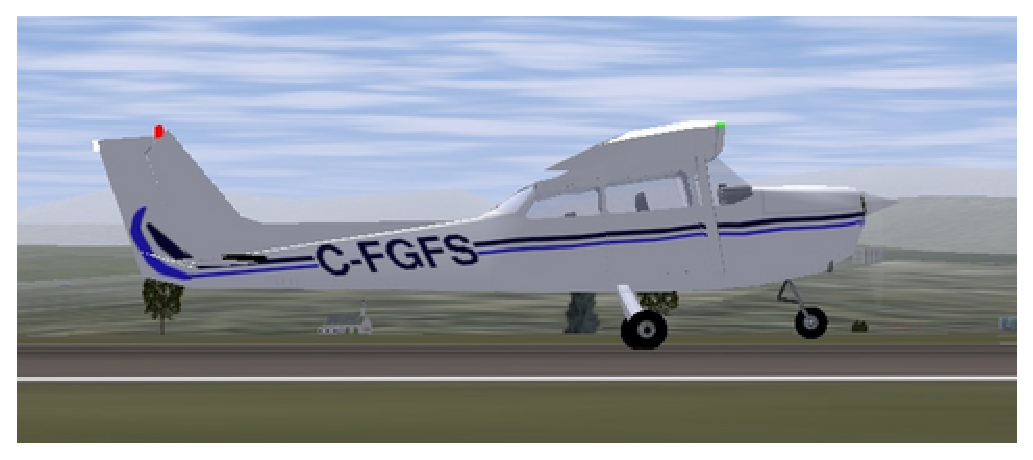
\includegraphics[width=0.5\textwidth]{img/tut_25}
\end{center}

The reason why you must raise the front wheel is it is not designed to
roll at high speeds. It would shimmy and wear out.

Question: if the front wheel no longer touches the runway, how do you
steer the airplane? Answer: still using the rudder pedals. The
rudder pedals are also linked to the tail rudder, that big vertical moving
part at the tail of the plane:


\begin{center}
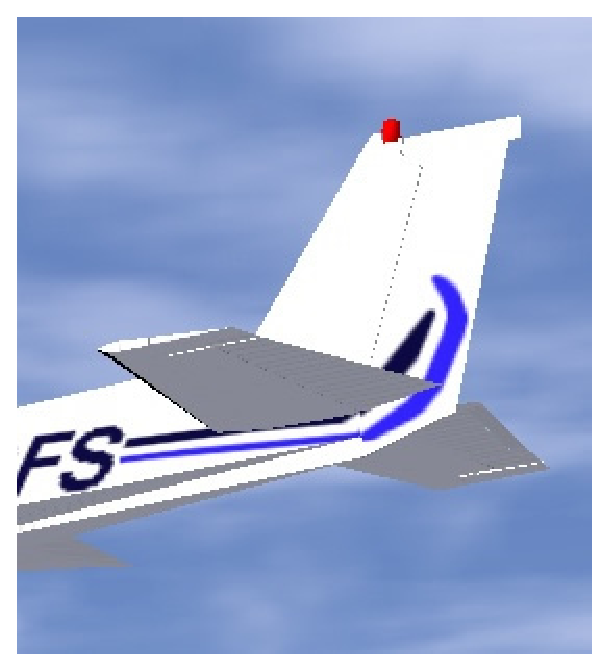
\includegraphics[width=0.5\textwidth]{img/tut_26}
\end{center}

At air speeds above 40 knots, the rudder is adequate to steer the airplane. 

The rudder pedals command both the front wheel and the rudder at the
airplane's tail. So, just move the rudder pedals...

Note the front wheel and the tail rudder don't make the airplane turn
exactly the same way. So when the rudder takes over the front wheel,
you must adapt the rudder pedals angle. That means fast typing keypad
\key{0} and keypad \key{Enter} (or hold the left mouse button down and
tightly control the rudder with the mouse).

Once you've become familiar with this, you will be able to keep the airplane 
straight on the runway during take-off.

Say the airplane is heading too much to the right. You type
keypad \key{0} a few times to make it turn back to the left. Don't
wait till the trajectory is corrected. Type keypad \key{Enter} before
the aircraft reaches the direction you wish to travel. Otherwise you will
find that you will over-correct. If you use the mouse, things are
much easier and more precise.

To summarise: two methods exist to steer the airplane on the ground: the
differential brakes on the side wheels and the rudder pedals. This 
control redundancy is very common in aviation. If one method fails, 
you still have another method available as an alternative way to perform 
the task. 

You may be wondering why the aircraft drifts to the left when it rolls on the 
ground, forcing your to compensate with a little push on the right rudder 
pedal? The main reason is the flow of air produced by the propeller. It 
blows along the airplane body, but also corkscrews around the airplane 
fuselage. The upper part of that slight vortex pushes the vertical tail 
to the right. This causes makes the front of the aircraft to head to the left.

You can center all yoke and rudder controls by typing \key{5} on the
keypad. This is a good preflight precaution. Sometimes it can ``save
your life'' in flight. 

\section{Turning in the air}
\label{sec:Turning}
    
As with turning on the ground, there are two methods of turning in the air. 
You can use the wing ailerons (steered by the yoke/mouse) or
you can use the tail rudder (steered by the rudder pedals / the
keypad keys /\key{0} and \key{Enter}.
    
Why these two ways? Partially for redundancy, but mainly because they are 
complementary. The main effect of the rudder is yaw, while the main effect
of the ailerons is roll.
    
\begin{itemize}
	\item When flying close to the ground, it is better not to bank the 
  airplane in order to turn. The rudder is used more instead. Acting on the 
  rudder pedals allows you to turn the airplane without excessive banking. 
	\item When the plane is close above the runway, the two side wheels need to 
  be at the same height above the runway for landing. That means the wings 
  must be level with the horizon. The plane is not allowed to bank. You keep 
  the plane wings level with the horizon by using the yoke/mouse/ailerons. 
  Note this does not need to be perfect. A bank of a few degrees is harmless.
	\item In flight, especially at high speed, the rudder is a dirty way to make 
  the airplane turn: 
\begin{itemize}
	\item It causes the airplane to present its flank to the airstream, increasing
  drag.. 
	\item The airplane will turn very slowly.
	\item You won't have very good control on the turn.
	\item At high flight speed the centrifugal force will be disturbing or even 
  dangerous.
\end{itemize}
Using the yoke/mouse/ailerons allows for efficient, fast, reliable and 
comfortable turns.
  \item The rudder can be vital when the wings are stalled. Indeed, during a 
  stall the wing ailerons become less effective or even useless. 
  (Note that some airplanes can go in a very dangerous stall if you overdo the 
  rudder control at low speed.)
\end{itemize}

When you turn in flight, using the ailerons, you still need the rudder 
a little bit. You add a little bit of rudder. This allows you to 
perfectly compensate for the adverse yaw created when you roll using the 
ailerons. In a real aircraft, you can feel this sideways motion. In the
simulator, you can check this visually on the turn coordinator. In the 
picture below the little ball is pushed rightwards during a strong turn 
to the right using the ailerons. That means you the pilot endure a rightwards 
force too. You can compensate this by pushing the right rudder pedal 
(type the keypad \key{Enter} key a few times). In normal flight you use the 
rudder to keep the little ball centered. 


\begin{center}
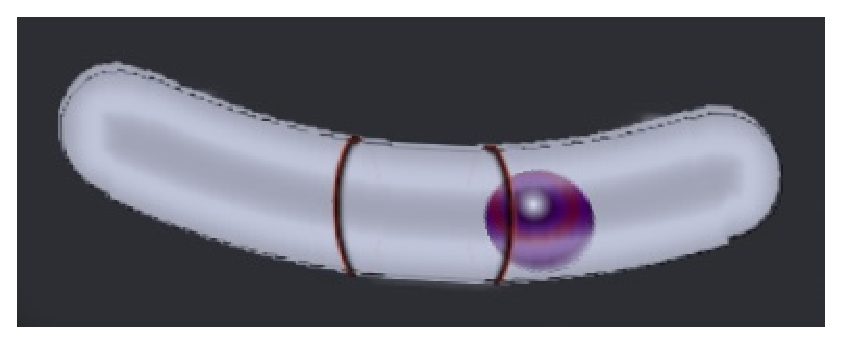
\includegraphics[width=0.25\textwidth]{img/tut_27}
\end{center}
  
So, you tend to turn by using the ailerons in normal flight and by using 
the rudder when close above the ground at low speed. Yet one method never 
completely cancels out the other. You still need the rudder at high altitudes 
and speeds. Reciprocally you have to use the ailerons a little bit when close 
to the ground, to keep the wings level with the horizon. 

Even when taxiing, you should use the ailerons. Otherwise, strong winds can
blow the aircraft onto its side. To counteract this, your should turn the
ailerons into the wind.

It is best never make quick and strong movements with the rudder. On the
ground at high speed this can make the airplane turn to sharply. In flight
at low speed it can cause a very dangerous stall. In flight at high
speed it can cause all kinds of aerodynamic and physical discomfort.
Instead, make gentle movements of the rudder. 

I recommend you train to turn with the rudder in flight. Fly at a low
speed of about 70 knots. Try to keep the altitude stable by increasing
and decreasing the engine power. Use the rudder to turn towards a ground
feature and maintain a heading, then turn the aircraft towards a new heading.
See how the plane yaws. Learn to anticipate rudder
control. Don't try to make steep turns. Use the yoke/ailerons to keep
the wings level constantly.
  
\section{A Bit of Wieheisterology} 
  
Wieheisterology comes from the German phrase ``Wie hei\ss t Er'' -- 
``What's that name''. This section is about gauges, switches and controls of 
the aircraft. It's like the buttons of a video game control pad: you can play 
a game with just the arrow buttons but if you want to get the fun out of the 
game and beat serious opponents you need to learn the functions of the other 
buttons. Equally, in the simulator, you can take off and land a basic airplane 
with just the engine throttle and the yoke but you need all the controls to 
perform securely and efficiently. You need to have at least a basic 
understanding of the physics behind the controls. In emergency situations you 
have to understand how the controls work to be able to cope with their 
deficiencies.

\subsection{Engine control}
\label{sec:EngineControl}
    
An airplane engine is a technological wonder. It is the most powerful, 
efficient, lightweight and reliable fuel energy plant commonly available.

On the bottom left, below the instrument panel you will find the 
\Index{magneto} switch and engine starter:


\begin{center}
\includegraphics[width=0.25\textwidth]{img/tut_28}
\end{center}

To see the switch, either type  \key{P} to get the schematic instrument
panel or type \key{Shift-x} to zoom out (\key{x} or \key{Ctrl-x} to
zoom back in).

You can move the switch with the \key{\{} and \key{\}} keys (use the \key{Alt
Gr} key on Azerty keyboards).

You are probably aware that the fuel inside a car engine is ignited by 
electric sparks. Modern car engines use electronic ignition. An airplane engine 
uses a more old-fashioned (but more reliable) magneto ignition instead. For
redundancy, it contains two such magnetos: the ``left'' one and the ``right'' 
one. When you cahnge the magneto switch on OFF, both magnetos are switched off
and the engine will not run. With the magneto switch on L you are using the 
left magneto. On R you are using the right magneto. On BOTH you use both. 
In flight you will use BOTH.

Given that you use both magnetos in flight, why have the switch? The reason
is that during your pre-flight checks you will verify that each of the magnetos
is working correctly. To do this, increase the RPM to about 1500 then switch 
the magneto switch to L and observe the tachometer. You should observe a 
slight drop in RPM. If the engine cuts out, the left magneto is broken. If 
you do not see an RPM drop, then the switch may be faulty, as both magnetos 
are still switched on. You can then perform the same test on the right magneto.
Of course, in the simulator, the magnetos are unlikely to fail!

Should one of the two magnetos fail in flight, the other one will keep doing 
the job. The failure of one magneto is rare, the failure of both together is 
almost unheard of.

You may have typed \key{\{} to shut the engine down. To start
the engine again after doing so, type \key{\}} three
times in order to put the magneto switch on BOTH. Then use the starter motor
by pressing the \key{Space Bar} for a few seconds, till the engine is started.

You can also turn the magneto switch and start the engine by clicking
left and right of the switch in normal mouse mod). Type \key{Ctrl-c} to
see the two click sides highlighted by yellow rectangles.

If you turn the switch to OFF, the engine noise stops. If you quickly
turn the switch back to L, the engine starts again, though you didn't
turn the switch to START. The reason is the propeller was still
rotating. You should have waited till the propeller came to a halt.
Then, placing the switch on L, R or BOTH won't start the engine. (Once
the engine is halted, always place the magneto switch to OFF.)

\subsection*{The throttle}\index{throttle lever}



\begin{center}
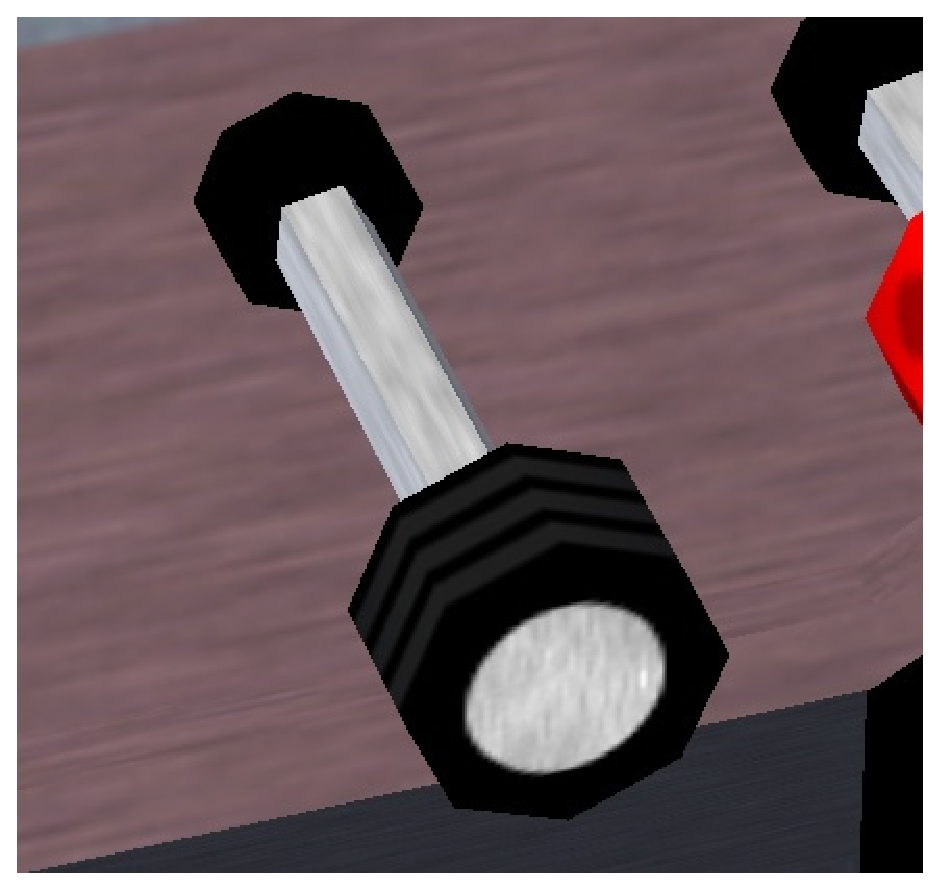
\includegraphics[width=0.25\textwidth]{img/tut_29}
\end{center}

You already know that you increase the engine power by pushing that throttle
lever in (\key{Page Up} key). You decrease the power by pulling the
lever out (\key{Page Down} key). You can also click left and right of
the lever (middle mouse button for quicker moves, \key{Ctrl-c} to
highlight the left and right halves).

What does ``increase the power'' actually mean? Does it mean you increase 
the amount of fuel delivered to the engine? Yes, but this is not enough to 
fully understand what you are doing. You need to be aware that the engine is
also fed with a huge amount of air. The engine's cylinders burn an
\Index{mixture} of fuel and air. Fuel alone wouldn't burn.
Only a mixture of fuel and air can detonate and move the engine
pistons. So when you push the throttle in, you increase both the fuel
and the air fed to the engine.

The amount of air compared to the amount of fuel is critical. The
proportion of the two has to be tuned closely. This is the purpose of
the mixture lever. The picture below displays the mixture lever, pulled out far
too much.


\begin{center}
\includegraphics[width=0.25\textwidth]{img/tut_30}
\end{center}

When the \index{mixture!lever} mixture lever is fully pushed in, you
feed the engine with an lots of fuel and little air. This is known as a 
``rich'' mixture. When the lever is pulled out completely, there is an 
excess of air, known as a ``lean'' mixture. The correct position to produce 
maximum power is in between these two extremes, usually quite close to fully 
pushed in.

When you start the engine and when you take off, you need a fuel-rich
mixture. That means the mixture lever pushed in. A fuel-rich mixture
allows the engine to start easily. It also makes the engine a little
more reliable. The drawback is that a part of the fuel is not burned
inside the engine. It is simply spilled away. This makes the engine
more polluting, it decreases the energy the engine can deliver and it
slowly degrades the engine by causing deposits of residues inside the
cylinders.\index{mixture!optimalisation}

Once in stable flight, you have to pull the mixture lever a little, to
get the optimal mixture. Check this out by doing the following. Start
the simulator. Put the parking brakes on with key B (that is
\key{Shift-b}). Push the throttle in to its maximum. The engine RPM are
now close to the maximum. Slowly pull on the mixture lever (using the
mouse in normal pointer mode). You will see the RPM increases a little.
You get more power, without increasing the fuel intake. You spill no
more fuel in the engine and it pollutes less. If you continue to pull
the mixture lever, the RPM will decrease back away, because now there
is too much air. The excess of air slows the explosions down inside the
cylinders and decreases the explosion temperature, hence the
thermodynamic yield decreases. You have to tune in the optimal mixture. For
thermodynamic reasons, the best mixture isn't exactly at maximum power - it
is better for the engine to be running very slight richer or leaner than
maximum power. You can find the maximum power point by the fact you get the
highest RPM. (Another method is to check the engine exhaust
temperature. Roughly, this is the point at which you get the highest temperature.)

The mixture control allows you to burn less fuel for the same speed and 
distance, and therefore fly farther and pollute less. It can also cause 
serious trouble. Suppose you go flying at high altitude and pull on the 
mixture lever accordingly. Then you descend back in order to land. 
If you forget to push the mixture lever in, The fuel/air mixture will become 
far too lean and the engine will simply halt. You may think the engine is 
failing and panic, while you only have to push the mixture lever back in\ldots

When landing, you have to tune back in a mixture that is a little too
rich in fuel. This means pushing the mixture lever in. That way the
engine becomes a little more reliable and will be better adapted to a
decrease in altitude.

I wrote above that placing the magneto on OFF is not the right way to
stop the engine. The right method is to pull the mixture
level\index{engine!right method to switch off}. First pull the throttle
out completely, to get the engine to minimum power and fuel
consumption. Then pull the mixture lever, till the engine stops because
the mixture contains too much air. This ensures the engine doesn't get
poised by spilled fuel residues. Finally, turn the magneto switch to
OFF to ensure the engine won't start back accidentally.

An important warning: you may think the RPM indicator reflects the
engine power. Wrong. Two things make the RPM increase: the engine power
and the airplane speed. To check this, fly to a given altitude
then pull the engine power to minimum. Try out diving to the ground
then rising back to altitude. You will see the RPM varies significantly. 
It rises while diving and decreases while 

One pitfall of this is when you intend to tune the engine power in for 
landing. Suppose you're
flying fast. You know the ideal RPM for landing is around 1,900 RPM. So
you pull the throttle till you get 1,900 RPM. You think you tuned in
the appropriate RPM. You think you shouldn't bother any more about it.
But now the plane's speed decreases. Hence the RPM decreases. A few
minutes later, you get the low flight speed you wanted. You don't see
the RPM is now at 1,000. Far too slow. You will either lose altitude or
stall. Or both. So, be cautious with the throttle and with the RPM
indicator. Either pull on the throttle more steadily or be mentally
prepared to push it back in quickly.

    \subsection{Wings and speed}
    \label{sec:WingsAndForce}
    
Fly with full engine power. Dropping the nose a little makes you lose altitude 
and raising the nose a little makes you gain altitude. You may think this is 
quite logical. The plane travels in the direction it is heading; the direction 
the propeller is heading. This is not the best way to think about it. 
This model would be fine for a rocket, but not for an airplane. A rocket is 
lifted by its engine, while a plane is lifted by its wings. 
That's a huge difference.

Get a big rigid square of cardboard, hold it horizontally in your hand
with your arm stretched out and make it do fast horizontal movements
while rotating your torso. When the cardboard moves flat through the
air, it experiences no lift force. If you twist your arm slightly to
give the cardboard a slight upward angle, you will feel it tends to
lift in the air. There is an upward force acting on the cardboard.
That's the way a wing holds a plane in the air. The wings have a slight
upward angle and lift the airplane. The more angle you give the
cardboard, the more lift force. (Till you give it too steep an angle.
Then you will rather feel a brake force. The cardboard is ``stalling''
(see below).)



\begin{center}
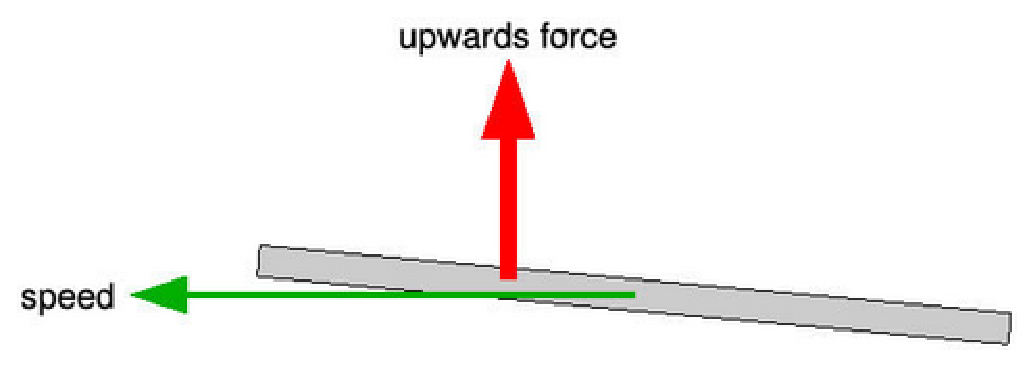
\includegraphics[width=0.5\textwidth]{img/tut_31}
\end{center}

\begin{itemize}
	\item When you pull the yoke, the airplane's nose rises up. Hence the wings 
  travel through the air at a steeper angle. Hence the lift force on the 
  wings is stronger. Hence the plane rises in the air.
  \item When you push the yoke, the airplane's nose dives. Hence the wings 
  travel through the air with less angle. Hence the lift force on the wings 
  decreases. Hence the plane descends.
\end{itemize}

What matters is the angle the wings travel through the air. This is the
angle of attach.

I wrote above that when the wings travel through the air with no angle of 
attack, they don't produce lift. This is false. It would be true if the wings 
were a flat plate like the cardboard. But they aren't. The wings are a
slightly curved airfoil. This makes them create lift even when traveling 
through the air at no angle of attach. Actually, even with a little negative 
angle of attack they still create a lift force. At high speed the airplane 
flies with the wings slightly angled towards the ground! 


\begin{center}
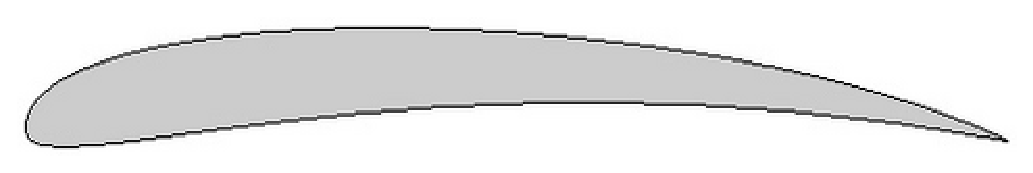
\includegraphics[width=0.5\textwidth]{img/tut_32}
\end{center}
    
The angle at which the wings travel through the air matters. Something
else matters too: the speed. Take the cardboard again in your hand.
Hold it with a given slight angle and don't change that angle. Move it at 
different speeds through the air. The faster you move the cardboard, the more 
upward force it experiences.
\begin{itemize}
	\item When you increase the engine power, the plane increases speed, the 
  lift force on the wings increases and the plane gains altitude.
	\item When you decrease the engine power, the plane decreases speed, the 
  lift force on the wings decreases and the plane loses altitude.
\end{itemize}

To make things a little more complicated: when rising in the air, the
airplane tends to lose speed. When descending, it tends to gain speed.

That's all a matter of compromises. If you want to fly at a constant
altitude and at a given speed, you will have to tune both the engine
power and the yoke/elevator (or better: the trim (see below)), till you
get what you want. If you want to descend yet keep the same speed, you
have to push the yoke a little and decrease the engine power. And so
on. You constantly have to act both on the engine power and on the
yoke. (During a normal flight one doesn't make things that complicated.
Simply tune in a comfortable engine power level then forget about it
and rely on the yoke and trim for the altitude.)

A very interesting exercise you can perform with the simulator is to
fly straight with full engine power. Get maximum speed while keeping in
horizontal flight. Then decrease the engine power to minimum. Pull steadily 
on the yoke to keep the plane at constant altitude.
The plane slows down steadily, meanwhile you have pull more and more on the
yoke to stay level. Since the speed decreases the lift of the wings 
would decrease, but you compensate the loss of speed by increasing the wing 
angle of attack. This proves the plane does not necessarily travel in the
direction its nose is heading. In this experiment we make the nose rise
in order to stay at constant altitude. Once the plane is flying very slowly, 
and the nose is very high, you may hear a
siren yell. That's the stall warning (see below). The angle of attack
of the wings is too high for the airfoil to produce lift. The wings are 
now braking the airplane instead of lifting it. The plane quickly loses 
altitude. The only thing you can do to correct this is push the
yoke forwards, making the nose drop, apply full power to gain speed and 
then bring the yoke carefully back to level flight.

Question: is it better to control the airplane's speed and altitude
with the yoke or with the throttle? Answer: it depends on what exactly
you intent to do and on the situation you are in. In normal flight, as
said above, you tend to set a comfortable engine power level, forget
about it and rely on the yoke and trim. During take off and landing the
procedures are quite strict about the use of yoke and throttle. You do
the opposite: control the speed with the yoke and trim, control the
altitude and descent speed with the engine throttle. That will be
discussed in sections below.

\subsection{The flaps} \index{flaps}
\label{sec:Flaps}
    
The flaps are situated at the rear of the wings, aside the plane's body:


\begin{center}
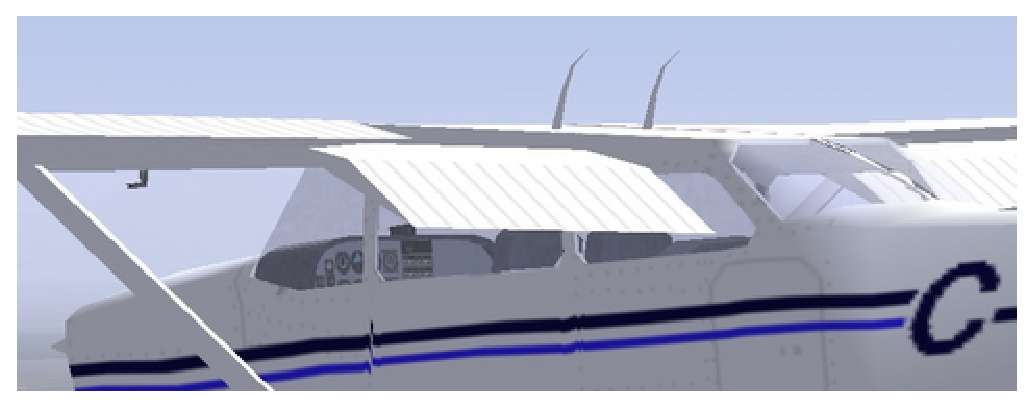
\includegraphics[width=0.5\textwidth]{img/tut_33}
\end{center}

Deploy the flaps and pull them back in by using the 
\index{flaps!control lever}flaps control lever:


\begin{center}
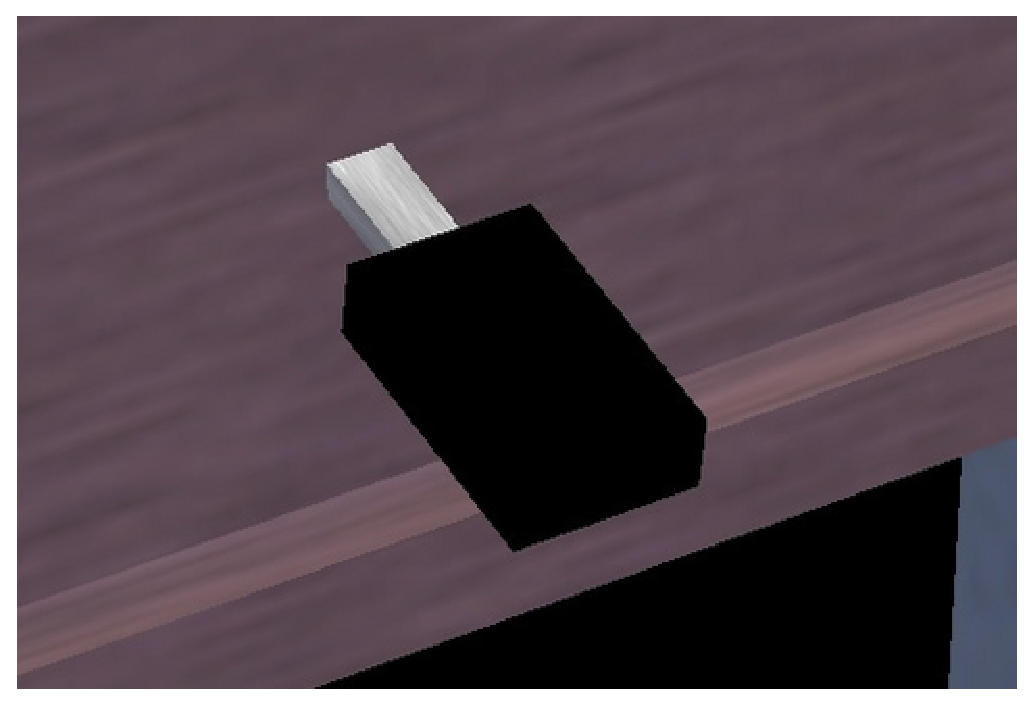
\includegraphics[width=0.25\textwidth]{img/tut_34}
\end{center}

You can either click on it with the mouse or use the \key{[} and
\key{]} keys. Key \key{[} to retract the flaps one step, \key{]} to
deploy them one step at a time. Type \key{v} to view the plane from the outside
and try out \key{[} and \key{]}. (On the schematic instrument panel the
flaps lever is located at the lower right.)

There are four \index{flaps!steps}flaps steps:
\begin{itemize}
	\item No flaps. For normal flight.
	\item One flaps step. For take off, when you want to gain altitude while flying slowly. Or during runway approach, while flying at constant altitude.
	\item Two flaps steps. To brake the plane, in order to lose altitude quickly, for example when you dive towards the runway to land.
	\item Three flaps steps. To lose altitude even more quickly. 
\end{itemize}
    
The flaps are somewhat delicate. Do not deploy the first step of flaps above 
110 knots. Do not deploy the second or third stage of flaps above 85 knots.

The flaps brake the plane at high speed. This is one more reason not to
forget to pull the flaps back in once you fly above 85 or 110 knots.

My favorite way to know the flaps position is to type
\key{Shift}-\key{right arrow}. Then quickly \key{Shift}-\key{up
arrow} to get back to front view. Another method I use is to make
sure the flaps are fully retracted by quickly typing [ several
times. Then type ] the exact amount of times needed.

Flaps increase wing lift by altering the shape of the airfoil. The wing lifts
more at a given speed with the first stage of flaps set. Hence you will get in 
the air a little sooner during take off. It also has the effect to make the 
plane fly with the nose a little more downward. This is handy: it allows to 
keep an eye on the runway while rising in the air. It also allows a better 
view on the runway during landing.

The flaps also incrase drag on the aircraft. The second and third stage of
flaps produce much more drag than lift, so they are used to brake the 
plane. This is particularly useful when landing, because the airplane glides 
very well. If you cut down the engine power completely, the plane will descend, yet
but too slowly. You need to deploy two or three flaps steps in order to
brake and really descend towards the ground.

The fact that the flaps brake during landing makes you need more engine
power during the landing. This can seem odd. Why not simply throttle
the engine down to minimum and use less flaps steps? The answer is that it is
better to have a strongly braking plane and lots of engine power,
as the plane reacts faster to your commands. Should the
engine fail, then just retract flaps as needed and your \ldots

Trying to take off with two or three flaps is a bad idea. This can
sound fun, but beware: suppose you deployed one flaps to take off. Yet
you forgot to pull the flaps back in. Later on you encounter a
emergency situation and you need to gain altitude very fast. You deploy
one flaps step. Actually you add one flaps step to the flaps step
already out. So now you have two flaps steps. Hence the flaps are
braking and you fail to gain altitude\ldots Whenever you feel the plane
is behaving really odd and seems unable to rise in the air, or even
keeps falling whatever your efforts and the engine power, think maybe
you deployed more than one flaps steps.

Redundancy\ldots What can you do if the flaps don't deploy and you
really need to brake? Answer: slowly push the rudder pedals on one
side. This will make the plane present its flank to the air stream and
brake. Compensate the turning by using the ailerons (yoke). This is not
a very comfortable way to brake and you should train it before using it
close to the ground. (I tried to use both the full flaps, the rudder to
an extreme and the throttle to minimum. You really loose altitude very
quickly\ldots)
    
    \subsection{The stall}\index{stall}
    \label{sec:Stall}
    
    
A \weblong{http://en.wikipedia.org/wiki/Stall}{stall} is an emergency
situation, at whatever altitude. It means the plane is flying too
slowly hence the wings travel through the air at too strong an angle.
The wings suddenly start braking the plane instead of lifting it. It is
especially dangerous when close above the ground. It is dangerous even
at high altitude because you lose part of your control over the plane.

During a normal flight, a stall should never occur. As a pilot you have
to constantly keep the plane well above stall speed. Once the stall
siren yells, it means things already have gone very bad.

Some little airplane like the Piper Cub are designed to land using a
near stall. Planes like the Cessna 172 are designed to make stalls less
likely to occur and less deadly when they occur. That's for example one
reason why the wing extremities are square. The Cessna is still
controllable during a stall and a simple stall and fast descent to the
ground should not kill the passengers. (Wind turbulences or a strong
bank can make things go worse\ldots)

A stall can make some airplanes go into a deadly
\weblong{http://en.wikipedia.org/wiki/Spin_(flight)}{spin}\index{spin}.
Fly for example the F-16 Falcon to some altitude, throttle the engine
down to minimum and pull steadily on the yoke to keep the same altitude
while decelerating\ldots One problem with the legendary WWII fighter
plane Spitfire was during too tight turns the inside wing would
suddenly stall completely but not the outside wing.

What can you do during a stall? The procedure can be very different on
different planes. You should not trust this tutorial, especially not
for such a serious matter. Anyway:
\begin{itemize}
	\item On little planes like the Cessna 172p or \index{stall!little planes}the Piper Cub you keep all controls on the airplane: elevator, rudder and both ailerons. Keep in mind the ailerons are on the wings and those wings are stalling. Think of using the rudder to turn. If you are very close to the ground, simply let the plane fall on the ground and keep it on the ground. Just try to make the best possible fall. If you are high in the air, push the yoke to dive the nose and gain speed. Think of retracting the flaps at one step. If possible, immediately add as much engine power as you can. Till you are out of danger.

	\item On the F-16, \index{stall!greater aircrafts}the ailerons loose all control during a stall. Actually that's the first sign of a stall: the ailerons act no more and the plane banks loosily. You only keep control with the rudder and the elevator. If the stall just begins, dive the nose and increase engine power. If the stall degenerated in a spin, engine power and dive won't solve the problem. Only the rudder will help to slow the spin down. Push the rudder to the other extreme of the spin direction. Push the yoke to help. Decrease engine power to minimum to get out of the spin more easily. Once the spin is slow enough, a dive and engine power will help. (If you put full engine power during the spin, you will loose less altitude I believe, but the spin's end will be difficult to control. React quickly to center the rudder again once the spin nearly stops, otherwise you will immediately go spinning in the other direction.) At low altitude you probably won't have the time to do all this. Note a spin with the plane belly up can happen too.


\end{itemize}

Stall-elegant airplanes like the Piper J3 Cub and the Cessna 172 tend
to have roughly rectangular wings. While stall-ugly airplanes like the
F-16 Falcon and the Cessna Citation II tend to have trapezoidal wings.
The advantage of the trapezoidal wings is they have a better
aerodynamic yield. They allow to fly more distance with a same quantity
of fuel. The ends of the rectangular wings engender strong turbulences.
Those turbulences brake the plane but also they keep the air flowing
correctly once the plane stalls...

When you learn to fly a virtual plane, making it stall is a very good exercise:

\begin{itemize}
	\item Fly at constant altitude with no engine power, till the stall begins. Then try to control the plane while it stalls and descends to the ground. Keep the yoke pulled to the maximum. Keep the plane in a steady attitude, the wings parallel with the horizon. Try to change direction. Experiment with the flaps. Note one flaps step decreases the stall speed. Two or more flaps steps don't change the speed much. Then end the stall by pushing the yoke and restoring engine power.
  \item Raise the nose in the air and bring the plane to a halt like a stone thrown upwards. Then try to get the plane back to normal flight.
\end{itemize}

Try to perform the exercices above with different airplanes. You will
notice how elegant the Cessna 172p behaves. First time I tried a stall
with the virtual Cessna Citation II, I was at 1,000 feet altitude,
which is supposed to be safe. The plane suddenly fell from the sky like
a tumbling stone. I was not able to stabilize the plane and it crashed.
I was really frightened by that airplane. On second attempt I managed
to stabilize before the plane hit the ground. Anyway, from now on I
won't fly a Cessna 172p and a Cessna Citation II with the same mood.

If you fly an unknown virtual airplane and wish to know the landing
speed, a rule of thumb is you find out the stall speed by
experimenting. Then you multiply that speed by a factor of 1.2 or more.
(A friend who is Aerospace Engineer told me 1.2.) The stall speed of
the Cessna 172p is 40 knots yet its imposed landing speed is 70 knots
(minimum 65 knots). That makes a factor of 1.75\ldots I made an
experiment landing the virtual Cessna 172p at 50 knots. It virtually
falls to the ground, at close to -1000 feet/minutes vertical speed.
This seems very hard for the landing gear. Next, while approaching at
50 knots with the Cessna 172p, the runway and most of the ground are
completely hidden. This obviously tells a higher speed is mandatory. I
would recommend following rules to find a correct landing speed. It
must be the lowest possible speed that satisfies all these conditions:
\begin{itemize}
	\item Be more than $1,2\times$ \hspace{-2pt}the stall speed.
	\item Be high enough to allow a vertical speed of no more than -500 feet/minute (all or most flaps steps deployed).
	\item On most modern planes, the landing speed must be high enough to allow you to see the runway while approaching at low speed and constant altitude.
\end{itemize}
On big jet airliners the flaps make a lot of difference. Bear that in
mind when you try to find the stall speed. Make the experiment with the
flaps deployed, as they will be deployed during the landing.

The load of the airplane also changes the stall speed a lot, and
therefore the landing speed. You land a fully loaded airplane at a
higher speed than an empty one.

(Once you get used to landing different airplanes, you get a feeling for the landing speed of an unknown airplane. You just feel the airplane "wants" to land at that speed. I suppose this is because the airplane was designed to land at that speed.)

\excl{In a real airplane the sounds and vibrations tell a lot about the state of the airplane. When all vibrations stop, this means you are going to stall. Then push the yoke to get speed.}

   
    \subsection{The trim}\index{trim}
    \label{sec:Trim}
    
    The trim is that dark big vertical wheel with gray dots located at the middle below the instrument panel:
    
    

\begin{center}
\includegraphics[width=0.25\textwidth]{img/tut_35}
\end{center}
    
  On \fg, the keys \key{Home} and \key{End} are used for the trim. The key \key{Home} rolls the wheel upwards while the key \key{End} rolls the wheel downwards. You can also click on the upper or lower half of the trim wheel (\key{Ctrl}-\key{c} for a yellow highlight). Possibly look at the plane from the outside (\key{v} or \key{V} and \key{x}) and move the trim while looking at the elevator.

In first approximation, the trim does the same as the yoke: it acts on
the elevator. Turning the trim wheel downwards is the same as pulling
on the yoke. Yet there is a key difference between the trim and a real
yoke. If you tune the trim, it keeps that tuning. While if you pull or
push on the yoke, it goes back to neutral once you release it.

Once in flight, you would keep the mouse/yoke at a given forward (or
backward) position. That position is optimal to keep the plane at a
roughly steady altitude. In a real airplane, this means you would
constantly keep pushing (or pulling) on the yoke. That would be quite
uncomfortable. This is where the trim falls in. You tune the trim to
impose a default elevator angle. Then you no longer have to push or
pull the yoke constantly. In other words: make a global rough tuning
with the trim and occasional fast tunings with the yoke/mouse.

The trim is an important control. I tend to forget it, for two reasons.
First is the mouse makes the trim virtually useless. This is quite
unnatural of course. People with a force-feedback joystick/yoke will
feel the need for the trim, as well as people flying real airplanes.
Second is the trim didn't operate on the particular version of
FlightGear I was using until recently\ldots

During take off the trim must be neutral. You have to check the trim is
centered before every take off. Also if you abort a landing and start
rising back to altitude, put the trim to neutral. Otherwise the plane
may buck.

During landing, while flying at a constant speed of 70 knots and a
constant altitude of 500 feet, the same applies as for a steady flight:
try to get the yoke/mouse/elevator towards neutral position by tuning
the trim. On the Cessna 172p this means trim on neutral (except when
the plane is loaded). On the Cherokee Warrior II this means the trim a
little ``pulled''.

During the final dive, some people seem to let the trim as it is and
use the yoke, others make the dive using the trim and don't use the
yoke/elevator. I don't know which is best. I use the yoke.

To know the trim position, use the HUD (\key{h}, \key{H} and \key{I})
or the I-shaped indicator on the schematic instrument panel (\key{P}).

The trim movement is very slow. Be patient.

Lots of modern airplanes have a remote control for the trim: a little
switch on the yoke, that you can manipulate easily with your fingers.
So you don't have to duck to roll the big wheel.

    
    \subsection{What direction am I flying?}
    \label{sec:Kierunek}
    
    Four basic methods exist to know what direction you are flying:
    
\begin{itemize}
	\item Look through the windows. Try to learn and recognize all sorts of ground features, like hills, bridges, cities, forests\ldots The Sun and the Moon are essential features, but clouds can cover them and they move through the sky. Looking through the windows can be quite hectic on a flight simulator. You only have a narrow view on the virtual outside world. Using two more displays, placed left and right of the main one, will help. Yet this is expensive and not mandatory. Several ways exist to allow you to pan your virtual head inside the airplane: 
	  \begin{itemize}
    	\item [$\rightarrow$]Use \key{Shift} and the four \key{arrow keys} to look frontwards, backwards, leftwards and rightwards.
    	\item [$\rightarrow$]Use \key{Shift} and the keypad keys to look in the four directions mentioned above and in four diagonal directions in-between
    	\item [$\rightarrow$]Put the mouse in pan mode (right button,  $\leftrightarrow$cursor look). This allows you to look in just every direction, including towards the sky and towards the ground. This method is great while the autopilot is on. It is a little dangerous otherwise, because the plane will bank or fall while you're looking all around. Click the left mouse button to quickly get back to the default forwards vision. Hint: if you click the left mouse button to center the vision back, by the time you click the right mouse button to go out of mouse look mode you will already have panned a few degrees away from the forward view. This is not a serious problem, except for the fact it prevents the instrument panel to appear when typing \key{P}. A solution is to lift the mouse before you click the left button. Then click the right button. Then let the mouse back down. (While the autopilot is on and you are looking all around, use the \key{x}, \key{X} and \key{Ctrl}-\key{x} keys to zoom in and out. Use the \key{z}, \key{Z} and \key{Ctrl}-\key{z} keys to dissolve the mist outside.) %
    \end{itemize}
  \item The compass (picture below). This is the indicator located above the instrument panel. The compass is a very simple and classical, yet not perfectly reliable instrument. When flying over some places, magnetic perturbations on the ground can make the compass tell nonsense. Also, the compass never shows the real direction of the North, East or South. Rather it shows a direction a few degrees aside from the real direction (depending on the country you are in). Close to the poles the error of the compass becomes really strong.  


\begin{center}
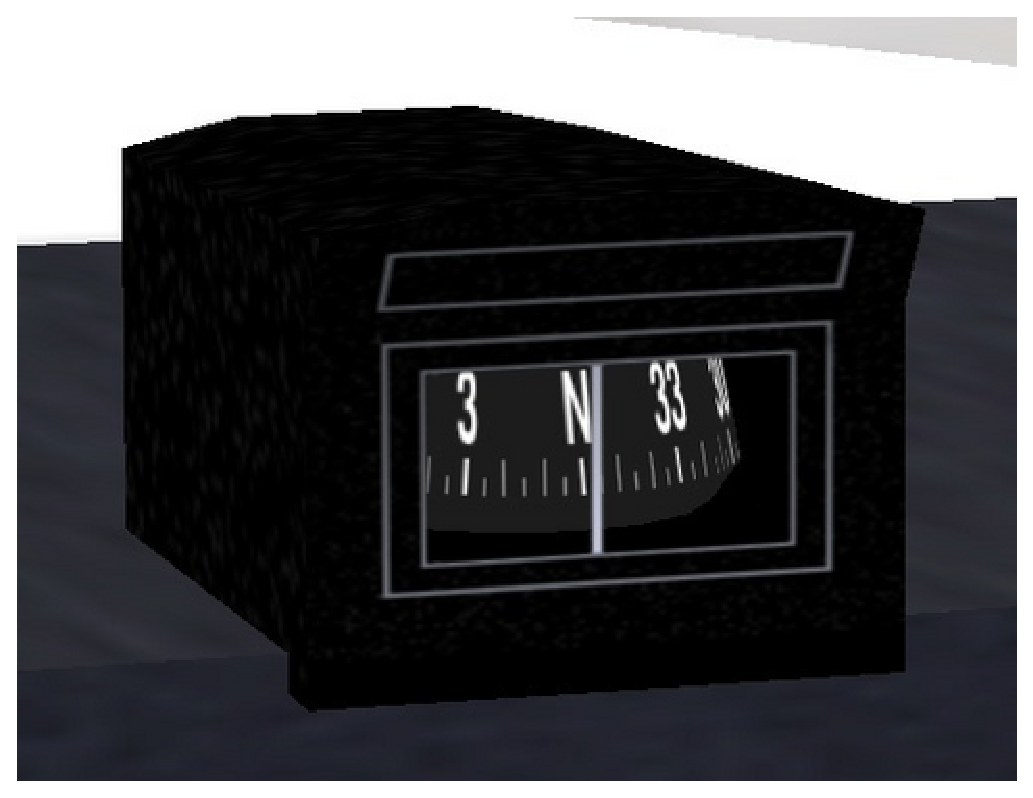
\includegraphics[width=0.25\textwidth]{img/tut_36}
\end{center}


  \item The directional gyro (picture below) or ``heading indicator''. The gyro is started before take off and keeps its initial heading for hours. It simply tells you how many degrees you turned to the left or to the right. You are supposed to tune in the right direction of the North Pole before you take off, using the knob at the bottom left of the instrument (normal mouse pointer mode, click left or right half of the knob, middle mouse button to move faster, \key{Ctrl}-\key{c} to highlight halves). (The red knob, bottom right, is used to tell the autopilot what direction you wish to fly (\textcolor{red}{\button{HDG}} = ``heading'').


\begin{center}
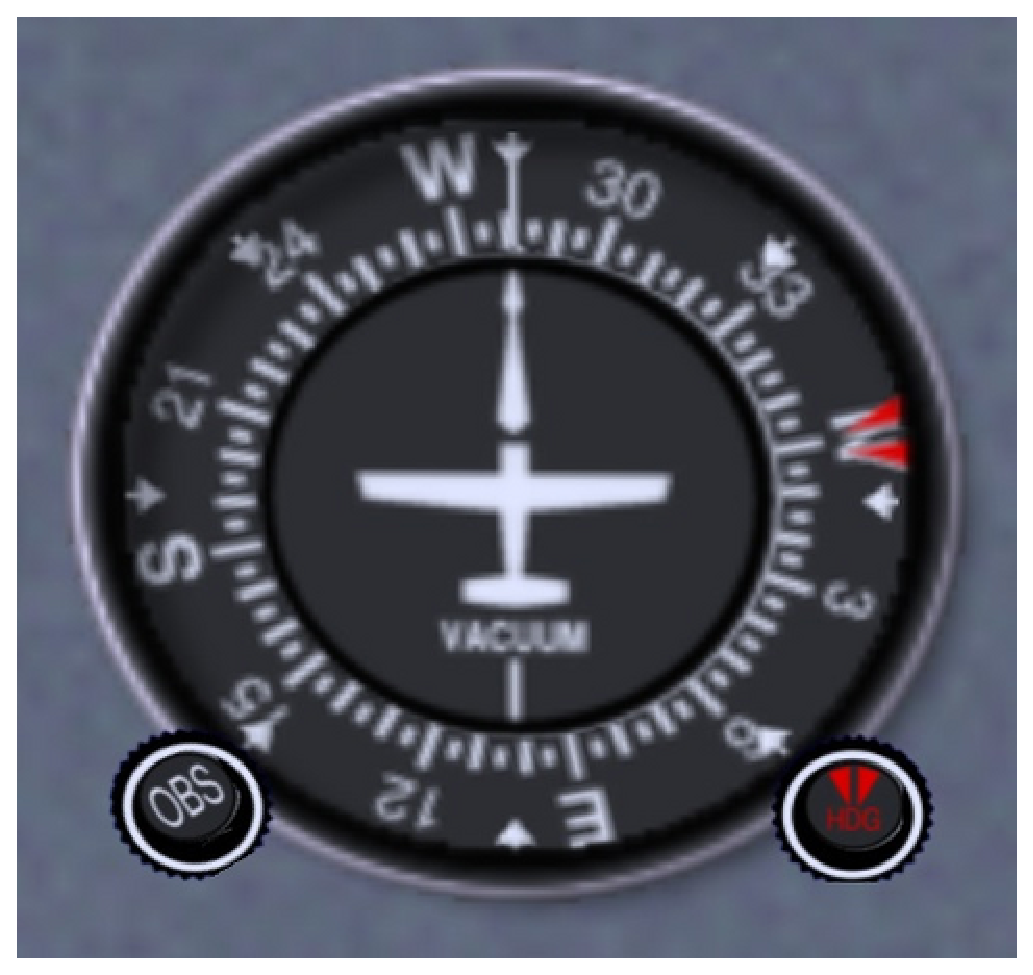
\includegraphics[width=0.25\textwidth]{img/tut_37}
\end{center}

  \item The clock. If you make steady turns, at the angle proposed by the turn indicator, a 180� turn takes 60 seconds whatever the flight speed (yet it is 50 seconds on FlightGear\ldots).

\end{itemize}    

  \excl{During a real flight in a real airplane, you are supposed to cross-check all direction indicators once in a while.}

Memorize the directions: North is 0$\textdegree$, East is
90$\textdegree$, South is 180$\textdegree$ and West is
270$\textdegree$.

  \section{Let's Fly}  
    \subsection{A realistic take off}
    \label{sec:Start}
    
By now I assume you are able to keep the airplane on the runway while
taking off (rudder) and you're able to fly straight, descend
peacefully, gain altitude steadily, make gentle turns (yoke)\ldots No
need you perform this all perfectly. Yet a basic and approximate
control of the airplane has been acquired.

Rules during \weblong{http://en.wikipedia.org/wiki/Take_off}{take off}: 
\begin{itemize}
	\item You are not allowed to keep the front wheel on the ground above 40 knots. It would shimmy.
	\item When close to the ground (I don't know the exact limit) you have to keep the two rear wheels at the same height above the runway. The reason is any moment you will or may touch the ground. You need to touch with both two rear wheels together. That means you need to keep the wings level with the horizon. Hence you cannot make use of the yoke/mouse/ailerons to turn. Instead you use the rudder pedals to turn. (Since you fly around 70 knots, this yields not too much sideways force problems.) The yoke/mouse/ailerons are used to keep the wings level with the horizon.
  \item You are not allowed to fly lower than 500 feet above the ground. The sole exception is in the axis of the runway, during take off and during landing. (While flying over cities you are not allowed to fly lower than 1,000 feet above the ground.)
  \item When lower than 500 feet above the ground, you are not allowed to fly \emph{slower} than 70 knots speed. That's because a blow of wind from the rear can occur any moment. You need to fly fast enough so that such wind blows won't make the plane stall and fall to the ground.
  \item When lower than 500 feet (above the ground), you are not allowed to fly \emph{much faster} than 70 knots. You wouldn't be able to make maneuvers quick enough. You would be more destructive if you hit something. Besides, 70 knots is a nearly optimal speed to gain altitude and your sole acceptable purpose while lower than 500 feet is to gain altitude\ldots
  \item While taking off, you must stay aligned with the runway. Indeed that's the sole place you are allowed to fly below 500 feet. (If you take off from a long runway like KSFO, this also allows to land back safely and quickly should an emergency occur. (Above a short runway, you cannot simply dive and get back on the runway, because it is too short. You need to turn and circuit to make a regular landing. For this you need to have enough engine power or to be at least at 500 feet above the ground. Otherwise, quickly find a place where you can make an emergency landing.)) 

\end{itemize}

So, you need to take off and rise in the air at a steady speed of around 75 knots.

Problem: since the front wheel is slightly lifted and the flaps are one
step deployed, the plane will rise from the ground already at 55 knots.
That's well below the desired flight speed of 75 knots. What to do
then? Answer: as soon the two rear wheels lift from the ground, push
the yoke forwards a little. Keep the plane close above the ground. (The
aim of this is: should a wind blow from the rear occur, the plane will
fall from only a few feet hight.) Keep it close above the ground while
accelerating, till a speed of about 70 knots is reached. Then switch to
the opposite mode: now you must pull on the yoke to prevent the plane
from going above 75 knots. Force the plane to rise in the air, so it
doesn't gain speed. Keep in control. If the speed goes below 75 knots,
push a little on the yoke. If it rises above 75 knots, pull a little on
the yoke. Till you reach 500 feet above the ground.

This is the procedure I use to take off. I assume you just started \fg; the airplane is at the start of the runway and the engine is turning at minimum power:
\begin{enumerate}
	\item Get a HUD ( \key{h}, \key{H}, \key{i} and \key{I}) or the schematic instrument panel with the I indicator (2D panel aircraft from start or key \key{P}).
	\item Deploy one step of flaps (\key{]}).
	\item Get in mouse yoke mode ($+$ pointer shape) by clicking on the right mouse button.
  \item Pull the yoke/mouse/elevator to 1/2 the total way: 


\begin{center}
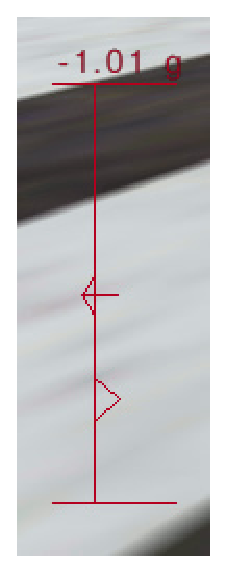
\includegraphics[width=0.25\textwidth]{img/tut_38}
\end{center}

  \item Ensure the yoke/mouse/ailerons is centered: 


\begin{center}
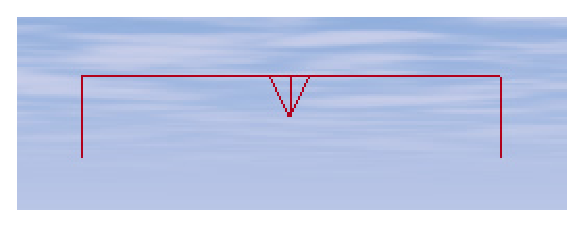
\includegraphics[width=0.25\textwidth]{img/tut_39}
\end{center}

  \item Push the left mouse button down and keep it down, so the mouse gets in rudder control mode. (If you don't want to use the mouse to control the rudder, use the keypad \key{0} and \key{Enter} keys.) (Before you push the left mouse button, ensure the yoke/elevator is pulled 1/2 like asked above and the yoke/ailerons is centered.)
  \item Keep the \key{Page Up} key down till the engine roars at its maximum power.
  \item The airplane is now accelerating. Move the rudder/mouse to the left and to the right to keep aligned with the runway (the left button is pressed). You need to keep in the middle of the runway but this does not need to be very precise. More important is your path is parallel with the runway middle line and stable. 
  
  \item Because the yoke/elevator is pulled $1\over2$ in, around 40 knots the nose will rise up. Immediately release the left mouse button, to get back in yoke control mode. Immediately push the yoke/mouse a little bit, to keep the engine cover below the horizon. You just need to let the front wheel rise a little bit above the runway. Let the rudder keep its angle (probably slightly turned to the right; two keypad \key{Enter} hits from the center position). From now on keep the left mouse button released, to stay in yoke control mode. Use the keypad \key{0} and \key{Enter} keys to control the rudder. (You can also make short presses on the left mouse button to make little rudder adjustments. I prefer using the keys.)
  
  \item The airplane soon leaves the ground. The two rear wheels no longer touch the runway. Push the mouse a little, to prevent the airplane from rising in the air. Keep it flying close above the runway and aligned with it. (Do not try to stick really close to the ground. This would be dangerous. Let the plane rise a little bit. Just do not favor the rising.)
  \item Use the yoke/ailerons/mouse to keep the wings level with the horizon. Use the rudder/keypad \key{0} and \key{Enter} to turn (needs training). Optimal rudder position seems to be slightly right from neutral; two keypad \key{Enter} hits.
  \item Once the airspeed reaches 70 knots, pull on the yoke/mouse a little bit. Now the airplane firmly rises in the air. If the speed gets below 75 knots, push the yoke to force the airplane to rise slower and gain airspeed. If the speed rises above 75, pull the yoke to rise faster and decrease the airspeed. There is no need to be very precise. Try to keep a stable speed. Just avoid to go below 70 knots and above 80 knots.
  \item Don't keep your eyes too much on the speed indicator while you are rising above the runway. Rather look at the horizon and at the engine cover. The top of the engine cover should roughly match with the horizon line:


\begin{center}
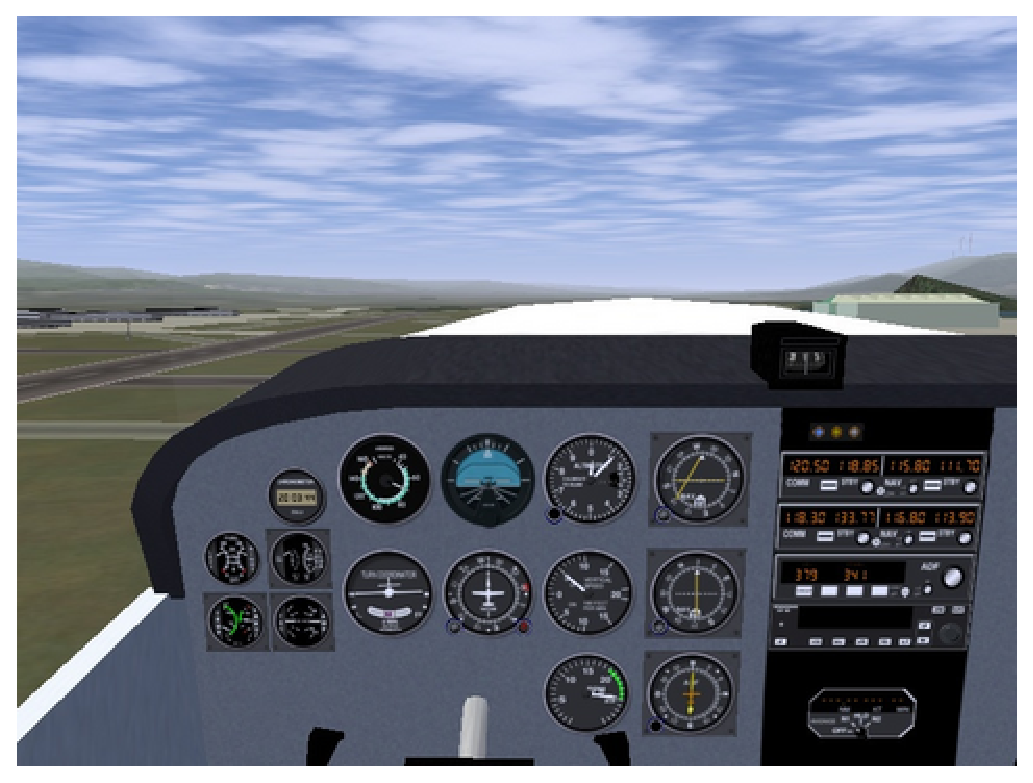
\includegraphics[width=0.5\textwidth]{img/tut_40}
\end{center}
  
  \item If you want to check the position of the runway but you can't see it because it is hidden by the engine cover, push the yoke/mouse a short while to make the nose dive a little bit for a second. This only works for long runways. Another trick is to look for a building, a hill or something far in front of the runway, on the horizon. Keep aiming at that object while rising in the air. Keep the engine cover a little below the horizon line, so the object you aim at stays visible.

  \item Once you reach 500 feet, retract the flaps (\key{[}) and push the yoke a little. Center the rudder (slowly, one step at a time). You are now allowed to gain speed or go on climbing (your choice, or the control tower's). Decrease the engine power a little so the RPM needle gets in the green zone (\key{Page Down}). Turn calmly towards your intended flight direction. Use your time to optimize the mixture. You're in flight.  
\end{enumerate}    
    
500 feet above the ground is the minimum flight altitude above open
land. Above a city the minimum altitude is 1,000 feet.

If you take off from KSFO heading to the West, you have city areas in
front of you and left of you. So, once you reach 500 feet above the
ground, best turn to the right.

Don't forget to center the rudder. If the rudder is pushed to one side,
this will brake the plane. It makes the plane move sideways through the
air, with its flank aerobraking.

Don't forget to retract the flaps.
    
    \excl{During a real take off you must keep in touch with the control tower. You also have to constantly look in all directions to check no other airplane is coming in your direction. }
    
An aviation classic is the
\weblong{http://en.wikipedia.org/wiki/Ground_effect}{ground
effect}\index{ground effect}. It's the fact a wing lifts better when
close above to the ground. That too makes the wheels leave the ground
at quite a low speed, a speed at which the airplane cannot really fly.
While you are accelerating a few feet above the runway, you are in
ground effect. If you know about it, ground effect is an advantage
because it makes flying close above the ground more secure. The
airplane behaves a tiny little bit like a hovercraft. If you are not
aware of the ground effect, it can cause problems. For example it can
make you think the airplane has enough speed to rise in the air, while
it has not.


    
    \excl{During a real take off, if the engine halts below 500 feet, you are not allowed to turn and try to glide and land back on the runway. You only have enough height to try to turn and land back if you are above 500 feet when the engine halts. }
    
    \excl{Before a real take off you have to go through check-lists. A checklists makes you verify, tune and tighten a list of items. You have to follow a long checklist before you enter the runway and a short checklist before you accelerate to take off.}
    
This is the checklist I follow when I take of the virtual Cessna 172p
on \fg. It is very short compared to a real checklist. Anyway I know I
can go into (moderate) trouble if I don't follow it. I had to build up
the discipline to follow it carefully each time:

\begin{itemize}
	\item Check the wind direction
	\item Deploy one step of flaps.
	\item Click the right mouse button and ensure the mouse is in yoke mode ($+$).
	\item Put on a HUD (\key{h}, \key{H}, \key{i}, \key{I}) or the schematic instrument panel  (\key{P}) in order to know the controls positions.
	\item Pull the yoke/mouse to $1\over2$ the pull path.
	\item Check the yoke/ailerons are centered.
	\item Keep the left mouse button down and check the rudder is centered or slightly to the right.
	\item Keep the  \key{Page Up} button down to start accelerating, till the engine RPM is maximum.
\end{itemize}

    
    \subsection{Landing}\index{landing}
    \label{sec:Ladowanie}
  
When I was a boy, I had a simple yet fairly good flight simulator on my
\weblong{http://en.wikipedia.org/wiki/ZX_Spectrum}{Sinclair ZX
Spectrum} home computer. I could do everything with it, except landing.
I always crashed the plane, or reached the end of the runway before
stopping. One day a real pilot saw me trying to land. He had never seen
a flight simulator, but he had no problem to recognize each flight
instrument and ground feature on the screen. He told me what to do.
Decrease engine power, increase engine power, push the nose down, pull
the nose up, turn a little left, turn a little right, get the flaps
out\ldots We made a perfect landing on the second attempt.
  
  Just like for take off, \weblong{http://en.wikipedia.org/wiki/Landing}{landing} is partly a procedure, partly rules you have to stick to. You have to adapt constantly.

  Same basic rules apply as for take off, yet in reverse order:
\begin{itemize}
	\item Stay at 70 knots once below 500 feet. Descend towards the \weblong{http://en.wikipedia.org/wiki/Runway}{runway} while keeping at 70 knots. 
	\item After the final rounding (see below), stay close above the runway while decreasing speed from the 70 knots flight speed down to the roughly 55 knots landing speed.
	\item Touch the runway with the two main wheels. Keep the front wheel from the ground till the speed is below 40 knots.
\end{itemize}

(If you know what you are doing you are allowed to use a speed a little below 70 knots: 65 knots.)

Following rules are essential during the whole procedure of landing:
\begin{itemize}
	\item Tune the speed using the yoke/mouse/elevator: push the yoke if you are flying below 70 knots, pull the yoke if you are flying above 70 knots. No matter this makes you gain or lose altitude (except when this causes a danger of course).
  \item Tune the altitude using the engine throttle. Add power if you are too low, retract power if you are too high.
  \item Once approaching the ground, use the yoke/ailerons to keep the wings level with the horizon. Turn using the rudder.
  \item Don't shut the engine down. Only shut the engine down when the airplane is completely halted on the ground. There are two reasons for this:
\begin{itemize}
	\item [$\rightarrow$] Any moment you may need full engine power to rise back in the air.
  \item [$\rightarrow$] Engine thrust enables you to make more precise landings. For example if you land on a very short runway, you need that precision.
\end{itemize}
\end{itemize}

The reason why the yoke/elevator is used to tune the speed is this
method allows for fast reactions and fine tuning. It is more important
to tune the speed closely than the altitude.

If you are both a little too high and a little too slow, simply push
the yoke a little and both problems will be solved together. No need to
use the throttle. Use your mind...

You have to get aligned with the runway. That means your flight
direction has to match the middle line of the runway (drawing (a)
below). In order to arrive at this, don't aim at the start of the
runway (b). Rather aim at a fictitious point well ahead of the runway
(c). And begin to turn gently towards the runway well before you reach
that fictitious point (d). Note the turns and bankings you make for
these flight corrections are often very soft. You wouldn't even notice
them on the turn coordinator. This is one example where you better rely
on the outside horizon line than on the inside flight instruments.


\begin{center}
\includegraphics[width=1.0\textwidth]{img/tut_41}
\end{center}

Try to get aligned with the runway as soon as possible. Constantly
apply the alignment procedure. The closer you come to the runway, the
better the alignment should become.

My favorite landing procedure for the Cessna 172p is roughly this one:
\begin{enumerate}
	\item Far from the runway, yet already heading towards it, start decreasing the speed and let the plane descend towards 500 feet. 
	\item Check the rudder is neutral. Otherwise the plane will be braking and more engine power is needed. (Type keypad keys \key{0} and \key{Enter} to center the rudder if needed.) If you make corrections using the rudder, keep in mind you may need a little more engine power.
	\item Once the speed is below 100 knots, deploy one flaps step  (\key{]}). 
	\item Once an altitude of 500 feet is reached, keep that altitude. Once a flight speed of 70 knots is reached, keep that speed. (If in doubt, keep above 500 feet.) The exact altitude doesn't matter much provided it is stable. But stick to 70 knots.  
	\item Be firm with the flight speed. Keep a tight and quick control on the yoke/mouse to keep 70 knots. If the speed is lower than 70 knots, push the yoke to gain speed (no matter you lose altitude). If you are above 70 knots, pull the yoke to lose speed (again, no matter this makes you gain a little altitude). Don't panic if the speed rises to 75 knots or decreases to 65 knots. But keep in mind you can really get in trouble if you approach a short runway at 80 knots. I manage to keep the speed between say 68 and 72 knots.  
	\item Tune the trim to get the average position of the yoke/elevator centered. This is not mandatory on the simulator, yet that way you better mimic piloting a real airplane. On the Cessna 172p (with no load) this means trim on neutral.
	\item Be firm with the flight speed. Keep a tight and quick control on the yoke/mouse to keep 70 knots. If the speed is lower than 70 knots, push the yoke to gain speed (no matter you lose altitude). If you are above 70 knots, pull the yoke to lose speed (again, no matter this makes you gain a little altitude). Don't panic if the speed rises to 75 knots or decreases to 65 knots. But keep in mind you can really get in trouble if you approach a short runway at 80 knots. I manage to keep the speed between say 68 and 72 knots.
	\item Fly at constant speed and steady altitude towards the runway. 70 and 500. Keep trying to align with the runway. You will \textbf{never} be perfectly aligned. You have to go on aligning till the airplane halts on the runway.
	\item Now you are at a low flight speed of 70 knots, no more use the ailerons/yoke to turn. Instead use the ailerons to keep the wings horizontal. Turn using the rudder (Keypad keys \key{0} and \key{Enter}). The rudder can seem an odd device for this purpose yet you will get used to it. Move the rudder only a few key hits to the right or to the left. Be patient. Make one key hit at a time and allow the airplane to stabilize before you possibly make another key hit. (When I started making landings, I found the rudder to be hectic and I prefered to use the ailerons to turn. As experience build up, I finally found out that turning with the rudder allowed for more precise and comfortable adjustments.)
	\item The airplane may oscillate a little. Don't bother. Just keep in control using the yoke.
	\item You're flying at constant altitude and 70 knots speed. Once the beginning of the runway passes under the engine cover, it's time to take things up seriously. This is shown in the picture below. (Whatever altitude you are flying, once the engine cover begins to eat the runway, you are at a correct angle towards the runway start.) 


\begin{center}
\includegraphics[width=0.5\textwidth]{img/tut_42}
\end{center}

	\item Type \key{]} two times, to deploy the full three flaps steps.
	\item Immediately push the yoke forwards, to make the airplane plunge to the ground. Indeed, the full flaps deployed make the plane brake. You plunge towards the runway to land, of course, but also to keep the speed at 70 knots. 
	\item Decrease the engine power. $1\over4$ the maximum is often fine. The Cessna 172p needs even less. I tend to decrease the engine power throughout the dive, to end with almost no power. The possibility to add engine power is necessary for your safety and for the precision of the landing, but also the possibility to decrease the engine power. So I try to make my dives a way that I keep the engine at some decent power level throughout the dive. If a dive obviously begins with the need to decrease the power to minimum, there is a risk you touch the runway far beyond its start.
	\item Watch the speed indicator like it if was your heartbeat. Control the speed using the yoke/elevator. 
	\item The dive makes you head towards the runway. You will soon become aware that the plane is going towards a point of the runway much further than the start of the runway. There is nothing wrong with that on a long runway. Yet you should train to land on short runways. In order to correct the dive and head towards the start edge of the runway, decrease the engine power. (On the Cessna 172p this often leads to power to minimum, while on most other airplanes you keep some power tuned in.) The picture below is a snapshot from a good dive. (Note the vertical speed indicator shows $-500$ feet/minute. I never use that indicator. I solely aim at the runway edge and its 12 white strips. Anyway, -500 feet/minute is the right descend speed\ldots) 


\begin{center}
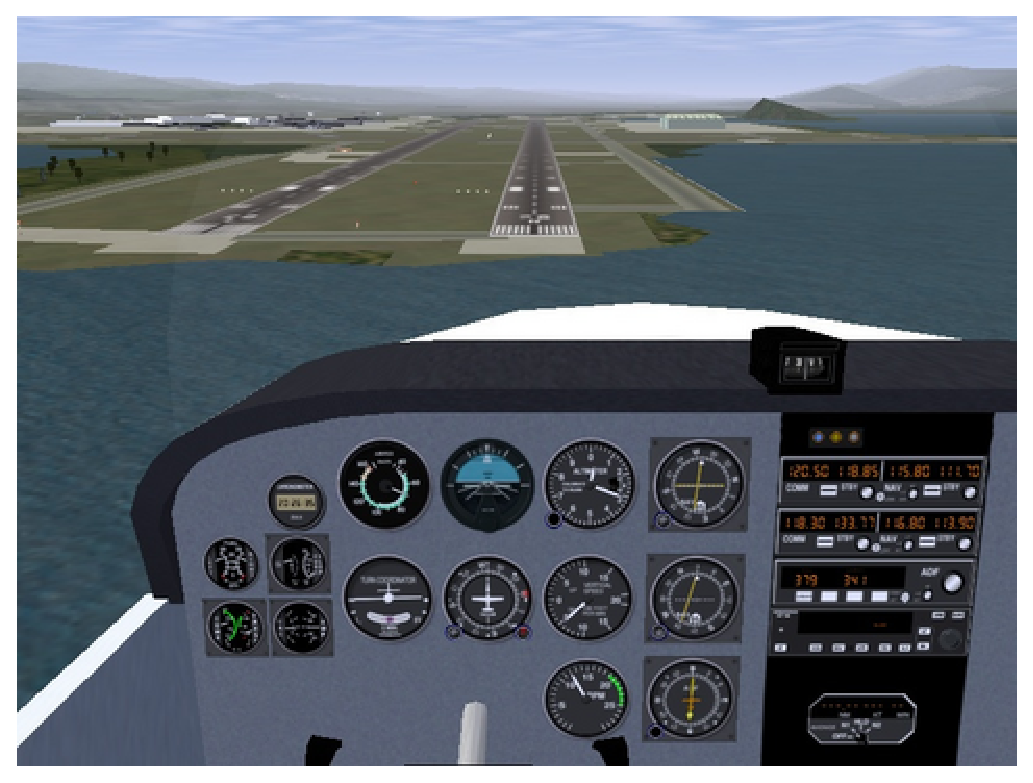
\includegraphics[width=0.5\textwidth]{img/tut_43}
\end{center}
  
  \item Closely keep the speed at 70 knots by pulling and pushing the yoke. Calmly increase and decrease the engine power in order to head the plane towards the starting line of the runway. Don't bother to aim exactly at the start of the runway. It doesn't matter if you arrive a few feet before the runway start or much further after it. Provided you arrive at 70 knots. 
  \item Keep aligning with the runway, using the rudder pedals to turn (keypad keys \key{0} and \key{Enter}). Keep the wings level with the horizon using the mouse/yoke/aile\-rons. (Use the ailerons to turn only if an emergency occurs and you need to make fast and steep turns. Then you probably need to abort the landing and get back to altitude (see below).)
  \item If you suddenly realize you will arrive really far before the beginning of the runway, possibly retract the flaps to one step (\key{[}). You can also let the engine roar to maximum power for a few seconds. If you followed the procedure you shouldn't need to do such extreme things\ldots (At any time, if you feel things are going wrong, retract the flaps to one step, throttle to full engine power, put the trim on neutral and gain back altitude (keep the speed above 70 knots). Whatever wrong happens -- you arrive aside from the runway, too far before the runway, at a wrong speed, a swarm of birds is passing, whatever -- abort the landing. Get back to altitude and retry.) 
  \item The ``\Index{rounding}'' is the most impressive part. You are like going to crash on the runway. Yet you will pull the yoke/mouse before it's too late. Don't pull on the yoke too early. Don't pull on the yoke too firmly. Once you are really close to the runway (for a beginner: once you are convinced it's too late and you are going to smash into the ground), pull the yoke gently and bring the plane in a steady flight above the runway. That's the rounding. (During the rounding, ground effect contributes to your security and ease.)
  \item It is often best to reduce the engine power to minimum during the rounding.
  \item Go on using the rudder pedals (keypad \key{0} and keypad \key{Enter}) to keep aligned with the runway. Use the yoke/ailerons to keep the wings level with the horizon (so both left and right wheels will touch the runway at the same time). 
  \item Now you're flying close above the runway (in ground effect). Throttle the engine power to minimum if it wasn't already done (this is mandatory). Deploy full flaps if they weren't already deployed completely (this is not mandatory on a long runway). (Don't shut the engine down. Just throttle to minimum power. It still can happen that you suddenly must take off again and need full power in a few seconds.)
  \item Keep the plane flying close above the runway. As the speed decreases from 70 knots down to 50 knots and below, keep pulling more and more on the yoke/mouse, steadily. Keep the plane in the air while ensuring it stays really close to the surface of the runway. Steadily lift the nose, while the plane slows down, up to quite a strong angle. Make sure the plane does not gain back altitude (don't look at the instruments, look at the outside). You really have to avoid the plane rises back in the air. Indeed it would do that at a speed below 70 knots... (You shouldn't need to pull the yoke more than $1\over2$ its maximum.) 
  \item Don't land the plane. Let it land by itself, once the speed is too low and the nose is high up in the air. The plane renounces to fly, it calmly sinks in and the two rear wheels touch the runway. If you don't hear the wheels hit the runway and the wheels nevermore leave the runway, you probably made an optimal landing. This also makes the front wheel stays above the runway while the two rear wheels touch.
  \item Once the rear wheels roll on the runway, retract the flaps. That way the wings will lift less and the plane will be more firmly on the ground. (My favorite way to land the airplane is to let the flaps down and keep pulling on the yoke while the airplane is rolling. That way I get maximum braking. I suppose this is an example of the difference between a simulator and reality. Using my way the airplane risks to get back in the air any moment and it is very sensitive to blows of wind. If I made real landings, maybe I wouldn't dare do this\ldots)
  \item When the plane is rolling, an optimal position for the yoke/elevator seems to be pulled $1\over2$ of the total way.
  \item Use the rudder pedals to keep the plane rolling in the middle of the runway and straight while the speed decreases. This most often leads me to two keypad \key{Enter} hits to the right of the center position.
  \item Once rolling at a speed below 40 knots, the nose will go down automatically. Help it by pushing the yoke/mouse calmly, back to neutral position. The front wheel now must touch the runway. Beware: check the rudder position first. If it is too much to the left or to the right, the plane will turn violently once the front wheel touches the runway. The plane may even fall aside and hit the ground with a wing tip. (The rudder slightly to the right; two keypad \key{Enter} hits, seems an optimal position.)
  \item Now the front wheel is on the ground, use the mouse to control the rudder. Keep the left mouse button down and forget the keypad keys. Maybe just check the ailerons and elevator positions are sound before you press the left mouse button. (Actually if everything went correctly and there is no crosswind, you shouldn't need to steer the plane using the rudder.) 
  \item Once the front wheel is on the ground, you are allowed to use the brakes. Your choice. Keep the \key{b} key down. Be prepared to release it should a problem occur. If you forgot to almost center the rudder, braking can go really bad.
\end{enumerate}

    Once the plane is halted or at very low speed, you can release the
    \key{b} key (if you used it) and add a little engine power to taxi
    to the parking or hangar.
 
    To shut the engine down:
\begin{itemize}
	\item Engine throttle to minimum (hold  \key{Page Down} down for a while).
	\item Pull the mixture lever to halt the engine (mouse in normal pointer mode, click on the left of the red mixture lever to pull it out).
  \item Rotate the magneto switch to OFF (a few hits on \key{\{}). 
\end{itemize}
To set the parking brakes in, type \key{B}.    
     
You must be mentally prepared to abort landing anytime. Whatever
happens: an order from the control tower, a wrong speed or landing
angle, a wrong alignment with the runway, a strong blow of wind, birds
flying over the runway\ldots retract the flaps to one, push the engine
to maximum, center the trim and get back to high altitude. Then either
you restart the landing procedure or you go for another airport. The
pride of a pilot is to make only safe landings.

Don't try to find ``the ideal distance'' to start diving to the runway.
The procedure above proposes you start diving when the white engine
cover starts eating the runway edge (provided you fly at 70 knots with
one flaps step) (the altitude doesn't matter). Best is you train to
land while starting the dive earlier and while starting to dive later.
You need to be trained to increase or decrease engine power according
to what is needed. During a real landing, depending on the airplane's
weight, the wind speed and other random things, the ``ideal'' moment to
dive is unpredictable. As experience builds up, you will better feel
the right moment.

If you want to make things simple for your first landing trainings,
make use of the fact the runway at KSFO is very long. Wait a little
more before you begin the dive: let the nose ``eat up'' the whole
length of the leading part of the runway (let the successive pairs of
white strips on the runway disapear below the airplane nose). Then
lower the flaps to three steps and decrease the engine to minimum. Dive
to keep the speed around 70 knots and try to keep aligned with the
runway. You will end the dive quite far beyond the runway start and at
a high vertical speed, but who cares. Make the final rounding. Keep
aligned with the runway and try to fly close above it. Keep pulling
more and more on the yoke/mouse, to keep the airplane flying. Yet avoid
it rising in the air. Till the wheels touch the ground. Then just keep
the airplane on the runway, using the rudder. Once the speed is below
40 knots, push the yoke/mouse and keep key \key{b} down to brake.

If you are a newbie, you probably won't succeed to apply the procedure
perfectly. My advice: invent your own, more simple procedure. Then
regularly come back to the procedure listed here and read it again, to
get hints and ideas to better your procedure. Till you get it. Also
best read other landing procedures. Send me a mail if you find
interesting differences. Analyze your own procedure. If it implies to
fly at very low speed, it is dangerous because a blow of wind from the
rear will make the plane fall. A probable problem with your procedure
is the plane needs a lot of runway length to land. If you look at the
runway start you will see there are successive groups of white stripes.
I land the Cessna 172 always well before the last group of stripes. If
you are a real beginner, your procedure surely will make the plane tilt
over or crash once in a while. The procedure listed here is safe. Train
your procedure, again and again. The more you train it, the more you
will become able to use the one listed here. That's the way I learned
to land\ldots

    \excl{In a real airplane, you must keep in touch with the control tower constantly while landing. You will be contacted by the control tower or you have to contact it in some key parts of the landing. If you don't contact the control tower just after landing, an emergency rescue team is immediately underway. If there is no good reason you didn't contact the tower, you will really be in trouble.}
    
    Maybe you'd like to train landing without having to take off and
    circuit in order to head for the runway and land. Type the command
    line displayed below in a terminal window to start the simulator in
    flight and heading for the runway. The airplane is placed 6 miles
    ahead of the runway, at an altitude of \textbf{1000} feet and a
    speed of about \textbf{120} knots.
    
    \command{fgfs --offset-distance=6 --altitude=1000 --vc=120}
    
    Possibly add   \command{--timeofday=noon --geometry=1024x768}
    jparameters if you need daylight and a bigger window (choose
    anything you need instead of $1024\times768$ (I favor
    $1200\times900$ an my screen)). FlightGear command line parameters
    are listed in \\
    \web{http://www.flightgear.org/Docs/InstallGuide/getstartch4.html\#x9-330004.4}
    
    (Note the parameters above make the airplane have some trim tuned in. Yet you need another trim tuning during the horizontal steady flight towards the runway. See the section \ref{sec:Trim} above, about the trim. If in doubt, just center the trim. On the Cessna 172p, a centered trim seems the right position.)
  
    Once you are trained, you no longer need to do a long horizontal
    flight at 500 feet and 70 knots to get to the runway. Instead you
    can descend all the way from your flight altitude and at a higher
    speed. You should be able to get at 500 feet and 70 knots a short
    while before the final dive.

Landing at 65 knots instead of 70 knots allows to use a much shorter
runway length. Yet to benefit from this you better train landing at 65
knots. It is quite different from landing at 70 knots.

The landing speed varies according to the load of the airplane. The
more load of petrol, passengers and freight, the higher the optimal
landing speed will be.

   \section{``My Friend the Wind''}
    \subsection{How to fly when there is wind}
    \label{sec:Fwsw}
    
    Think of a
    \weblong{http://en.wikipedia.org/wiki/Hot_air_balloon}{hot air
    balloon}. Think of it as being in the middle of a gigantic cube of
    air. The cube of air may move at high speed compared to the ground,
    anyway the
    \weblong{http://en.wikipedia.org/wiki/Balloon_(aircraft)}{balloon}
    itself is completely static in the middle of the cube. Whatever the
    \weblong{http://en.wikipedia.org/wiki/Wind}{wind} speed, persons
    aboard a hot air balloon experience not the faintest blow of wind.
    (To pilot a hot air balloon you bring it at an altitude where the
    wind blows in a direction that more or less suits your needs.) The
    same way, an aircraft flies in the middle of a gigantic cube of air
    and only refers to that cube of air. The motion of the cube of air
    compared to the ground doesn't bother the aircraft.

You, the pilot, on the contrary, do bother for the speed of the
surrounding air compared to the ground. It can make you drift to the
left or to the right. It can make you arrive at your destination much
later or much sooner than planed.

When the wind blows in the same direction as you fly, the speed of the
wind adds itself to the airspeed of the plane. Hence you move faster
compared to the ground. You will arrive earlier at your destination and
have less time to enjoy the landscape. (It sometimes happens that a jet
airliner flying with a strong wind from the rear, moves faster than the
speed of sound compared to the ground. Though it doesn't brake
the\index{sound barrier}
\weblong{http://en.wikipedia.org/wiki/Sound_barrier}{sound barrier}.)

When the wind blows in the opposite direction you fly (towards the nose
of the plane), the speed of the wind subtracts itself from the airspeed
of the plane. Hence you move slower compared to the ground. You will
arrive later at your destination and have more time to enjoy the
landscape. (Some slow airplane flying against strong wind can even seem
to fly backwards, because the speed of the wind is faster than the
flight airspeed of the airplane.)
    
    The two cases above are quite simple. More complex is when the wind
    blows towards the side of the airplane. Look at the pictures below.
        
\begin{itemize}
	\item On picture (a) there is no wind. The pilot wants to reach the green hill situated to the North. He heads for the hill, towards the North, and reaches the hill after a while. When there is no wind, you just head towards your destination and everything's fine.
	\item On picture (b), the pilot keeps heading to the North. Yet there is wind blowing from the left; from the West. The airplane drifts to the right and misses the hill.
	\item On picture (c), the pilot keeps heading towards the hill. This time he will arrive at the hill. Yet the plane flies a curved path. This makes the pilot loose time to get to the hill. Such a curved path is awful when you need to make a precise navigation. (Note something: the airplane tends to get into the wind, like a \weblong{}{weather vane}.)
	\item Picture (d) shows the optimal way to get to the hill. The plane is directed to the left of the hill, slightly towards the West. That way it compensates the wind and keeps on a straight path towards the hill. It will need more time to reach the hill than if there was no wind, anyway this is the best attitude. (Note something: the solution is to let the airplane head a little bit into the wind, like a weather vane would.) 
\end{itemize}
    


\begin{center}
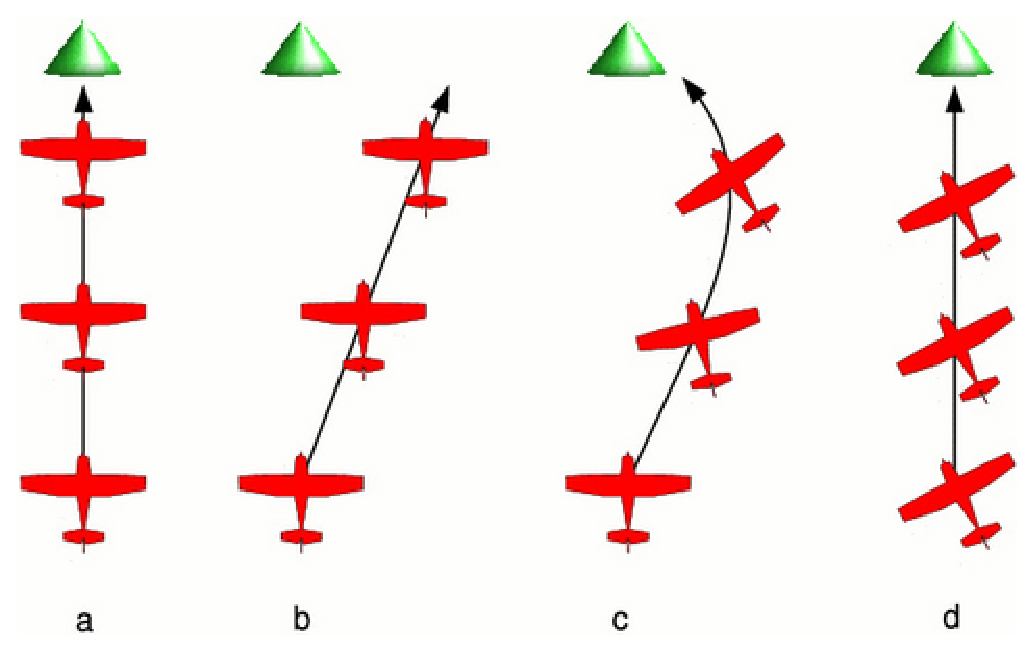
\includegraphics[width=1.0\textwidth]{img/tut_44}
\end{center}

How much to the left or to the right of the object must you head? At
what angle? Serious pilots use tight geometry and trigonometry
computations to get near exact and optimal angles. Yet I wouldn't fly a
virtual Cessna 172p if I had to do such dry things. You need no
computations at all to fly roughly straight. The trick is you must keep
your eyes on the object you fly towards. You know you will head the
plane in a direction to the left or to the right of the object, but you
don't need to know the angle. Just keep your eyes on the object. Get
aware you are drifting leftwards or rightwards. Then let your instinct
slowly head the plane to the right or to the left to compensate the
obvious drift. When you begin training this, you need to force your
instinct a little bit and think of what you are doing. Very soon this
will become automatic, just like when you learned to fly straight. You
will no more keep the plane headed towards the object. You will rather
keep it flying towards the object. The picture below shows a flight
towards the top of the little mountain ahead. Wind blows from the
right. I just look at he mountain top. And I let my hands head the
plane to right of the mountain, without really thinking about it:


\begin{center}
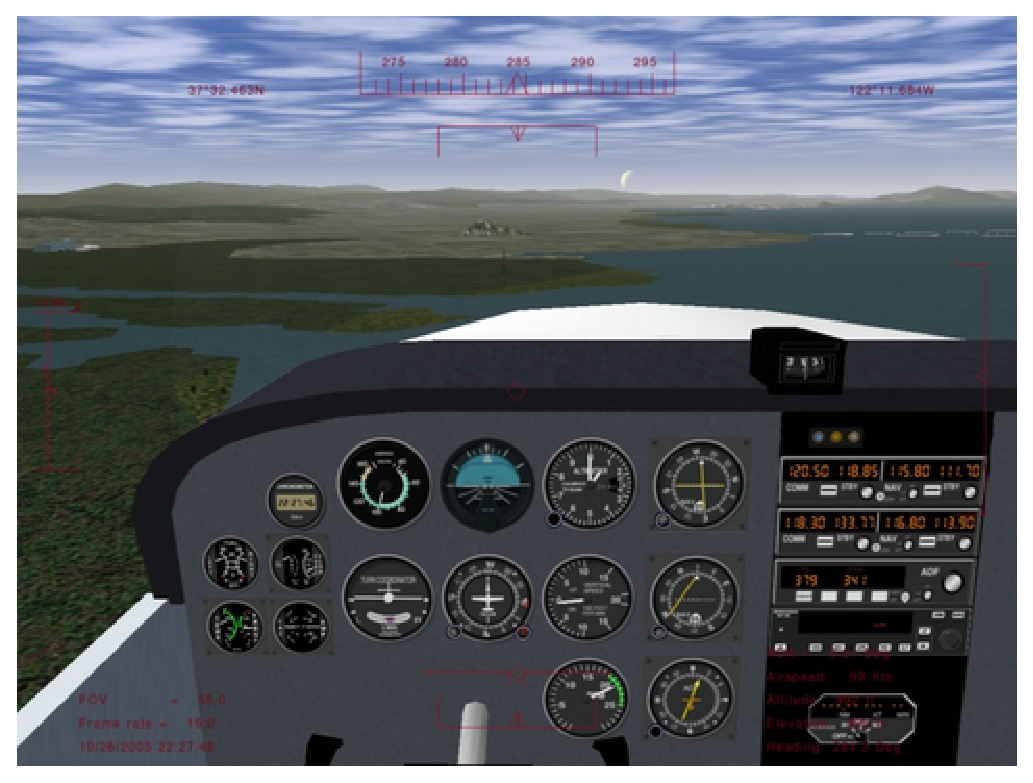
\includegraphics[width=0.5\textwidth]{img/tut_45}
\end{center}
    
    The faster the flight airspeed compared to the wind speed, the less the wind will influence.
    
    \subsection{How to take off when there is wind}
    \label{sec:Swsw}
    
Main recommendation to take off is you must find a way to accelerate
facing the wind; with the wind blowing towards the nose of the
airplane. Before most runways are build, statistics are made about the
wind at that location. The runway orientation is chosen so it aligns
with the wind most often. Lots of
\weblong{http://en.wikipedia.org/wiki/Airport}{airports} have two
runways at different orientations because the wind sometimes blows in
one of these directions and sometimes in the other direction. The
location of an airport is often chosen because at that place the wind
often has a stable direction and speed.

    
    Take off with a faint wind blowing towards the rear of the
    airplane, say 1 knot, for sure is no problem. Yet above a few knots
    you can get into trouble. With a 10 knot wind blowing from the
    rear, the front wheel will rise at the usual 40 knots airspeed, but
    that makes 50 knots compared to the runway. What matters is the
    speed the front wheel roll over the runway, not the airspeed... If
    a problem occurs and you are still rolling at 60 knots on the
    runway, the consequences will be more dramatic. To end with, you
    will need much more runway length and have less opportunities to
    abort the landing.

The main way to know the wind direction and speed is to go to the
control tower or ask the control tower by radio. A necessary and
complementary tool are the
\weblong{http://en.wikipedia.org/wiki/Windsock}{windsocks}\index{windsock}
at both ends of the runway. They show the wind direction and speed. The
longer and the stiffer the windsock, the more wind there is. The
windsock on the picture below shows an airspeed of 5 knots:
    

\begin{center}
\includegraphics[width=0.5\textwidth]{img/tut_46}
\end{center}

So, you have to choose a runway start that allows you to take off with
the airplane facing the wind. In real life you are not always allowed
to do this. Either there is no runway aligned with the wind or the
control tower tells you to use another runway. Then you have to take
off under crosswind; the wind blowing towards a side of the airplane.

Basically, you can use the exact same procedure as listed above for a
take off when there is no crosswind. Yet you have to be aware of
several important facts listed below. To train this, start FlightGear
with the parameter \command{--wind=0@10} which implies a wind of 10
knots blowing from the North (direction 0). If you take off from the
usual San Francisco KSFO airport heading to the West, this makes the
wind blow from the right.


\begin{itemize}
	\item You will have to push the rudder at quite a strong angle to stay rolling aligned with the runway. Keep the rudder at that angle once the front wheel leaves the ground and a little later once the rear wheels leave the ground.

  \item Say the wind is blowing from the right. You would think you have to push the right rudder pedal, to head the airplane a little bit into the wind, to compensate for the leftwards push of the wind. Well you have to do the exact opposite: push the left rudder pedal. This is quite unnatural yet that's life. The reason of this is the rear vertical stabilizer is pushed by the wind leftwards. The plane reacts like a weather vane and heads in the wind. The plane as a whole turns to the right, with quite a strong force. You have to compensate by pushing the rudder to turn to the left. So, you take off with the ruder pedals pushed to the left. The picture below shows a rudder angle during a take off with a 10 knots crosswind blowing from the right:



\begin{center}
\includegraphics[width=0.5\textwidth]{img/tut_47}
\end{center}

  \item The airplane will tend to bank leftwards. Hence you will have to push the yoke/ailerons to the right. Actually you best place the yoke a little to the right before the wheels start leaving the ground. (Best is to push the yoke to the right from the start on. Indeed this is the best way to taxi safely under a crosswind blowing from the right.) The picture below shows an appropriate yoke/ailerons position, while taking off with that 10 knots crosswind blowing from the right.


\begin{center}
\includegraphics[width=0.5\textwidth]{img/tut_48}
\end{center}
  
  \item The airplane will rise in the air much slower. The vertical speed will be quite weak. This is because the rudder is at a a strong angle. The airplane moves through the air with its right flanc and brakes. You have to wait till the rudder is centered before you get the regular vertical speed. Center the rudder very slowly, a little angle step at a time. Meanwhile, using the yoke/ailerons, gradually head the airplane a little bit in the wind, to keep flying aligned with the runway. Wait till you are above a few hundreds feet before you start centering the rudder.
    
\end{itemize}   

    Why do you keep the yoke to the right and the rudder pedals to the
    left once the airplane rises in the air? This can seem odd. It's
    quite logical that way the airplane will fly straight. The ailerons
    and the rudder compensate each other and the airplane turns neither
    to the right, neither to the left. But again, why do this, why not
    simply let the yoke/ailerons and the rudder centered? The airplane
    will fly straight too and be far less braked. The reason why we do
    this is the ailerons keep the airplane banked to the right; towards
    the direction the wind is blowing from. Hence, the huge force on
    the wings, that keeps the airplane in the air, that huge force is
    now slightly directed to the right. In normal circumstances this
    would make the airplane move slowly sideways to the right, at 10
    knots speed... Currently, it compensates for the 10 knots wind and
    keeps the airplane above the runway. So despite the wind, the
    airplane stays headed towards the runway end and stays above the
    runway middle. Everything's fine (except for the braking).

To me, 10 knots wind is a maximum to take off the Cessna 172p safely.
 

    \subsection{How to land when there is wind}
    \label{sec:Lwsw}
    
    You land the Cessna 172p under crosswind the same way you take off:
      
\begin{itemize}
	\item Try to land with the wind blowing towards the airplane face. Bear in mind the wind blows the airplane away from the runway start. So start the dive later, when the engine cover already ate some length of the runway.
	\item Under crosswind, use the exact same rudder and ailerons tuning as for take off under the same crosswind. Train this by taking off and landing under crosswinds. When the wheels leave the ground and you find the appropriate yoke/ailerons angle, note down the rudder angle and the yoke/ailerons angle. Center the rudder and ailerons during the flight and make a circuit to land back. During the landing, when you fly at constant 500 feet altitude and 70 knots speed, knowing the crosswind is the same, tune in back the rudder and ailerons angle that where optimal during take off.
\end{itemize}
  
  Under high crosswind, hence with a strong rudder angle, the plane brakes a lot. This implies two things:   
    
\begin{itemize}
	\item During the approach to the runway, at constant 500 feet altitude, 70 knots speed and 1 flaps step, you need much more engine power to keep the altitude stable.
	\item Once you dive towards the runway start, keep in mind the plane is braking. So you don't need to deploy additional flaps steps. Just decrease the engine power. 
\end{itemize}
   
    Landing that way is quite comfortable, despite the crosswind. You
    just have to be a bit more careful with the rudder once the
    airplane rolls over the runway. And best keep the ailerons as if
    turning towards the wind.

Note such a landing, with a steady crosswind, is unrealistic. In the
real world the wind varies quickly. You get sudden increases and gusts
of wind. The control tower just tells you by radio the maximum speed of
the gusts. You have to adapt constantly during the landing, to react to
the turbulences and gusts.

As for the take off, 10 knots wind seems a maximum to me. (Should you
ever have to land under heavy wind, say 25 knots or more, and there is
no runway aligned with the wind, maybe best don't land on the runway.
Or don't try to align with the runway. Align exactly with the wind and
make use of the fact you need less ground length to stop. When the
plane is going to stop keep the rudder pushed. Don't try to taxi.
Simply push the parking brakes in, push the trim and get help to latch
the airplane to the ground. In fun mode, landing the Cessna 172p under
70 knots wind is great. You simply let it descent to the ground
vertically. This is quite unrealistic because at such a wind speed
there are tremendous turbulences close to the ground.)

The technique described here is the
\weblong{http://en.wikipedia.org/wiki/Slip_landing}{slip landing}.
Another crosswind landing technique is the
\weblong{http://en.wikipedia.org/wiki/Crab_landing}{crab landing}.

    
    \subsection{How to taxi when there is wind}	
    \label{sec:Twsw}	
    
    Under 10 knots wind the Cessna 172p seems not to need particular precautions when taxiing. Yet any sudden increase in wind speed can tilt it and tumble it over. So best apply the recommendations whenever there is wind. 

To train taxiing on the ground when there is wind, ask for a strong
wind like 20 knots. Such a wind can tilt the plane and blow it away
tumbling any moment. One single error during taxiing and the plane is
lost.

Main rule is you must \emph{push the yoke towards the wind}. This deserves some physical explanation: 
\begin{itemize}
	\item When the wind is blowing from 12 o'clock, this is quite logical. The yoke is pushed (towards 12 o'clock) and the elevator makes the tail rise a little. That's the most stable position to avoid the plane be tilted by the wind.
	\item When the wind comes from 10 o'clock, pushing the yoke towards 10 o'clock makes the elevator is close to centered. The elevator almost no more trades in. Now the most important part is played by the ailerons. The left aileron is upward and the right aileron is downward. This pushes the left wing down and lifts the right wing. Again, that's the most stable position to avoid the plane be tilted by the wind. 
  \item When the wind blows from 8 o'clock, you would think you should invert the position of the ailerons, to keep the left wing being pushed down. Hence you should push the yoke to 4 o'clock. Wrong! Keep pushing the yoke to 8 o'clock. The reason is the downward position of the aileron on the right wing makes it act like a \weblong{http://en.wikipedia.org/wiki/Slats}{slat}. This increases the lift on the right wing and this is all we want. Symmetrically, the upward position of the left aileron decreases the lift of the left wing.
  \item When the wind comes from the rear, from 6 o'clock, the yoke is pulled (towards 6 o'clock). The upward position of the elevator tends to make the tail be pushed down. Once again this is the best. Strong wind can push the tail against the ground. This is impressive but the tail is conceived to withstand this.
\end{itemize}
    
    Accept the plane nose can be tilted and the tail pushed against the
    ground. Keep cool. This can be impressive yet there is nothing
    dangerous with it. Go on using the brakes, rudder and engine to
    move the airplane.

If you want to move towards the wind, you will need more engine power.
When the wind blows from the rear you may need no engine power at all.
Always keep the engine power to the minimum needed.

Especially when turning, move very slowly. Make little changes at a
time. Take your time and closely survey the yoke angle. Constantly keep
it pushed towards the wind. Constantly try to reduce the engine power.
Keep in mind using the brakes too firmly may shortly tilt the plane at
an angle that allows the wind to tilt it and blow it away.
 
    \section{The autopilot}\index{autopilot}
    \label{sec:Autopilot}
    
    An \weblong{http://en.wikipedia.org/wiki/Autopilot}{autopilot} is not an ``intelligent'' pilot. It just takes over simple and wearing parts of your work as a pilot. You still are the sole real pilot aboard and have to keep aware of everything. Be prepared to shut the autopilot down. During take off and landing, relying on the autopilot would be suicidal, because you have to keep an immediate control on every function of the airplane. (Dumb autopilot systems are reported to cause less accidents than smart ones with artificial intelligence inside.)
    
    The autopilot is that little rack to the right of the yoke:
    

\begin{center}
\includegraphics[width=0.5\textwidth]{img/tut_49}
\end{center}

Switch it on by pressing its  \button{AP} button (standard mouse mode).
The autopilot then controls the \index{autopilot!modes!roll control
mode}roll. It keeps the wings level with the horizon. This is displayed
in the picture below by the ``\textcolor{orange}{\button{ROL}}''marking.
To switch the autopilot down press again on \button{AP}.


\begin{center}
\includegraphics[width=0.5\textwidth]{img/tut_50}
\end{center}

If you press the  \button{HDG} button the autopilot will try to keep
the plane flying towards the direction tuned on the directional gyro by
the red marking (see the section \ref{sec:Kierunek} about
\index{autopilot!modes!direction mode}direction). 
``\textcolor{orange}{\button{HDG}}'' stands for ``heading''. Press
again on the \button{HDG} button to get back to roll control mode (or
\button{AP} to switch the autopilot down).


\begin{center}
\includegraphics[width=0.5\textwidth]{img/tut_51}
\end{center}

The buttons \button{ALT}, \button{UP} and \button{DN} are used to tell
the autopilot either to control the vertical
\index{autopilot!modes!vertical speed mode}speed
\textcolor{orange}{\button{VS}} or the altitude
\textcolor{orange}{\button{ALT}}.
    
From here on you maybe better study the document used by the author of the autopilot system in FlightGear\index{autopilot!author's documentation}: 
\\[6 pt]
 \weblong{https://www3.bendixking.com/servlet/com.honeywell.aes.utility.PDFDownLoadServlet?FileName=/TechPubs/repository/006-18034-0000_2.pdf}{https://www3.bendixking.com/servlet/com.honeywell.aes.utility\\.PDFDownLoadServlet?FileName=/TechPubs/repository\\/006-18034-0000\_2.pdf}
    
    \section{Security}
    \label{sec:Bezpieczenstwo}

Security is first of all a matter of common sense. Avoid to land with
the landing gear retracted. Fill the reservoirs before take off and
don't let them get empty in flight. This may seem funny
recommendations, the fact remains I made several landings on the
aircraft belly when I started using the flight simulator. I got angry
on myself and now it nevermore happens that I forget such a simple and
essential thing. In real life you are not allowed to land airplanes on
the belly in order to get angry on yourself. I suppose it is a part of
the role of the monitors to make you feel the angriness \textbf{before}
your first solo landing. I suppose they don't let somebody fly on his
own till they feel the angriness is rooted deeply enough in him. People
who cannot cope with this are not meant to become pilots.

There are much more vital details than the landing gear and the fuel. That's why checklists exist. There are checklists for all kinds of normal or emergency situations. There a long checklists and short checklists. This link provides checklists for the Cessna 172p and for other airplanes: 
  \web{http://www.freechecklists.net/}.   Those checklists refer to much more levers, buttons and triggers than talked about in this tutorial. There is nothing complicated in those checklists provided you learned what all those little things are. For example one item is you have to verify the seats backs are upright.

  You have to learn to cope with stress. Wherever I get access to computers I try to install \fg. To me the computer industry should focus solely on building computers for \fg. Secundary tools like browsers, mailers, spreadsheets and the like, should be regarded as optional sub-functions of \fg. Once the installation is finished, I make a demo flight. Strangely, most people simply don't care about what I am doing. They just go on talking, asking questions, requesting my attention\ldots What's more I'm often not in the most adequate position toward the screen, the keyboard and the mouse. It becomes almost impossible to fly correctly, especially to land. Basically there are two possible attitudes. The first one is I get silently angry on the disturbing persons, I stop the demo and I consider it's their fault if I cannot succeed my flight. The second attitude is I breath deeply and calmly, I find ways to go on managing the burdens and the problems, I don't get angry on anybody, I claim nothing to be responsible for anything, I renounce to make a perfect demo flight and I focus on making a mediocre yet secure landing. The advantage of the first attitude is that you feel comfortable about your superiority on \fg{}-unaware persons. The disadvantage of the second attitude is that you have to endure the humiliation of an ugly landing and the people around going on talking and requesting your attention. The advantage of the second attitude is that in real life, on a real airplane, it allows you to stay alive.

Communication is a basis for security. That means communication with
the technicians, with the control tower, with your copilot, with the
passengers and especially with yourself. You have to constantly gather
data about the traffic, the meteorology and the state of mind of your
passengers. You have to constantly inform the control tower and obey
the instructions it sends you in return. You have to keep your
passengers in an acceptable mood and at the same time you have to
obtain they let you focus on your tasks when this is necessary. Lots of
airline accidents occured because of a lack of communication between
the pilot and other crew members. That has been called ``the Superman
syndrome''. Once the problems start, the pilot focuses on his way to
solve the situation. Either the copilot does not understand what the
pilot is doing or he becomes aware of a danger the pilot did not
realize. This results in contradictory commands sent to the airplane
controls, shouting, up to fist fighting\ldots till the final crash of
the airplane. An important part of the training for modern pilots is to
learn to communicate with the other crew members under high stress.
They learn to go on communicating and how to do that a short and
efficient way. (I was once told this anecdote: a monitor and a trainee
were performing landings. The trainee was a strong guy with muscles
like truck tires. At one moment the landing path appeared to be wrong.
The monitor asked the trainee to release the commands so he could take
them over. There is nothing wrong with failing a landing. Monitors
themselves sometimes fail a landing, abort and restart a new landing.
But the trainee panicked and crispated his hands on the yoke. The
monitor could do nothing. The consequence was a damaged landing gear.)

There is no room for luck in real aviation. When you train to become a
pilot, almost every possible situation is put into practice at least
once. For example a monitor makes you take off with a heavily loaded
airplane and suddenly shuts the engine down. You have to train to fly
and land with a random airplane control or indicator out of order.
\fg{} allows to reproduce some of these trainings. You can request
flight instrument failures using \fg{}s' menus or command options. A
really bad instrument failure means the instrument still seems to
operate correctly. Yet it doesn't, and what it does or displays
endangers you. While training you can decide to no more use a given
instrument or control. For example you can glue a sticker on your
screen to hide away an instrument. Best is you ask a friend to
configure a failure without you knowing what he did. This heavy
training and the numerous precautions and rules are the reason why so
few accidents occur. In most cases, even a severe problem does not lead
to an accident. Accidents are often due to the unlucky addition of
several different problems.

The picture below shows the artificial horizon indicator. I hardly
never use it. I fly looking at the real horizon. Anyway the artificial
horizon saved me more than once on the simulator. When you penetrate by
mistake in a cloud or a bank of mist, you suddenly get a white outside.
There is no more way to keep the plane flying level, except by using
the artificial horizon. You may argue this due to the lack of feedback
own to the simulator. You're (dead) wrong. The same problem occurs on a
real airplane. Quite many of the (very few) accidents in little
airplanes like the Cessna 172 or the PA-28 happen that way. It is
prohibited for a pilot with no IFR license to enter a cloud. Some do it
anyway. Or they get caught in a rise of mist the control tower didn't
warn for. The airplane banks and in two minutes time it goes flying
upside down. The pilot is unaware of this. Even worse: some instruments
seem to get mad, with no obvious reason. A crash is unavoidable. I
learned the reflex to focus on the artificial horizon, the altimeter
and the directional gyro. When this happens the plane is often already
severely banked. I keep calm and I use the instruments to maintain the
plane in a sound flight. It will oscillate a lot but serious problems
will be avoided. Either I will wait till I get out of the cloud or I
will gain or loose altitude to get out of the cloud layer. I strongly
advice you train this using the simulator. Best is you make a complete
IFR training.


\begin{center}
\includegraphics[width=0.25\textwidth]{img/tut_52}
\end{center}

  One thing you have to train for your security is landing on very
  short distances.\index{landing!very short distance} Some flight
  incidents, like an engine failure or a sudden change in the weather,
  can force you to land on the first strip of flat land you encounter.

The \index{HUD (Head Up Display)} HUD allows to fly and land more easily, with less stress. It also allows to optimize what you are doing and this is good for security. For example it allows to touch the ground very close after the beginning of the runway. That way you have the whole length of the runway to brake. (A HUD is available for every aircraft on FlightGear, even the 1903 Wright Flyer. In real life, few little civil airplanes contain a HUD. It is too expensive and too recent.)

There are some strong differences between a flight simulator with minimalistic control hardware and a real airplane. The fact the mouse exerts no counterforce, the fact you don't feel the vibrations and forces inside the airplane\ldots On one hand, some aspects of flying are made easier on the simulator. On the other hand, a real airplane constantly gives all sorts of valuable feedback you don't get with a simulator. One thing is common to the simulator and the real airplane: while landing you'd wish you had four arms and two more brains.

\fg{} contains bugs. Consider those problems as a training for real aircrafts. Problems on real aircrafts are not the same. But there are problems. When \fg{} suddenly puts you in a critical situation due to a bug, consider this as a training. Try to solve the situation fast and efficiently while keeping calm. It's not a bug, it's a feature!

The handbooks of airplanes contain procedures and checklists for
emergency situations. It sometime happens that the adequate reaction to
a problem is exactly the opposite for two different airplanes. That's
one reason airline pilots are not allowed to fly different airplanes at
the same time\index{aircrafts change}. If they choose to go flying
another type of airliner, there are imposed to stop flying for a
lengthy period, during which they will practice the other type of
airplane on simulators. The wide range of aircrafts available under
\fg{} allows you to experiment with this.
  
    \section{What then?}
    \label{sec:Poslowie}

Once you master the content of this tutorial, you can claim to have a
basic understanding of what piloting is about. You still lack key
knowledge and training, like these:
\begin{itemize}
	\item How to follow real checklists.
	\item How to make emergency landing on very short fields, possibly with no engine power. 
	\item How to \weblong{http://en.wikipedia.org/wiki/Navigation}{navigate} according to the rules, charts, laws, radio beacons and crosswinds.
	\item How to draw a \weblong{http://en.wikipedia.org/wiki/Flight_plan}{flight plan}.
	\item How to place the loads in an airplane to get a correct center of gravity.
	\item How to deal with the \weblong{http://en.wikipedia.org/wiki/Control_tower}{control tower} and with other airplanes.
	\item How to deal with several fuel reservoirs and their valves, pumps and backup pumps. If two reservoirs are located on the wings ends and you let one of them empty while the other keeps full, you will get severe problems. 
	\item How to deal with the failure of every possible part of the plane. 
\end{itemize}

You probably will learn to deal with a retractable
\weblong{http://en.wikipedia.org/wiki/Undercarriage}{landing gear}
system and with variable pitch
\weblong{http://en.wikipedia.org/wiki/Propeller}{propellers}.

Go to the \fg{} documentation page for more tutorials and reference
pages: \\ \web{http://www.flightgear.org/docs.html}

These are great tutorials to learn further:
\begin{itemize}
	\item \weblong{http://www.flightgear.org/Docs/Tutorials/crosscountry/tutorial.html}{http://www.flightgear.org/Docs/Tutorials/\\crosscountry/tutorial.html}
	\item \web{http://www.navfltsm.addr.com/}
\end{itemize}

I wish to thank:
\begin{itemize}
	\item Benno Schulenberg who corrected lots of mistakes in my English in this tutorial. 
	\item Albert Frank who gave me key data on piloting and corrected technical errors.
	\item Vassilii Khachaturov who learned me new things about \fg. 
	\item Roy Vegard Ovesen for pointing me to the official Autopilot Pilots Guide. 
	\item Dene Maxwell for his solution for problems under Windows Me. 
	\item Mark Akermann and Paul Surgeon for their remarks. 
	\item Michael ``Sam van der Mac'' Maciejewski who made the translation in Polish and converted the tutorial in usable \TeX{} format.
	\item The \fg{} mailing list users for their hearty welcome. 
	\item \weblong{http://www.4p8.com}{4p8} webmaster my friend Fr�d�ric Cloth for the web space used by this tutorial. 
\end{itemize}

\section{`Pilots Fly Not Only On Cessna'}
\label{sec:NieSamaCessnaPilotLata}

I cross-checked all the data about the Cessna 172p, a friend who is a
pilot verified I did not write too blatant crap and I made numerous
virtual test flights. This appendix contains less reliable data about
other airplanes. It can be helpful as an introduction to those airplanes
but keep in mind my only goal was to make flights that seem OK and
acquire basic knowledge. You need other sources if you want to pilot
these airplanes a serious way.

    \subsection{How to land the Cherokee Warrior II}
    \label{sec:Cherokee}
    
    On Linux you get the Cherokee Warrior II (or PA-28) with the   \command{--aircraft=pa28-161} command line parameter. The Cherokee Warrior II has some advantages upon the Cessna 172p. Thanks to its low wings it is far less sensitive to crosswind. Fully extended flaps are more braking and allow to land on a much shorter distance. 

Take off is the same as for the Cessna 172p (in \fg. In real life their take off checklists are not exactly the same). 

You have to get used to some minor differences of the Cherokee Warrior II for the landing:

\begin{itemize}
	\item During the steady horizontal flight before landing, the trim must be pulled a little below neutral in order to get the yoke oscillating around neutral.
	\item The optimal tachometer RPM during landing is at a lower RPM than the tachometer green zone. Roughly, keep the needle vertical.
	\item Only put one more flaps step (which makes two flaps steps deployed) when the dive towards the runway begins. Don't decrease the engine throttle too much.
	\item If you keep it to two flaps deployed during landing, the hover above the runway and the final roll will be similar to the Cessna 172p. Yet if you put the third flaps step in (after the final rounding), the plane will brake firmly. It will very quickly touch the runway then come to a near halt. Be prepared to lower the front wheel very soon. (It is possible to use the third flaps step during the dive towards the runway, instead of tuning the engine power down. Oscillating between two steps and three steps allows to aim the runway start. Yet keep two flaps steps and tune the engine seems easier. An interesting stunt is to fly stable till nearly above the runway start, then tune the engine to minimum and deploy three flaps steps. The plane almost falls to the runway. It's impressive but it works.)
\end{itemize}
    
(In real life, an advantage of the Cessna 172p upon the Cherokee
Warrior II is the fuel reservoirs of the Cessna are located in the
wings close above the center of the plane and higher than the engine.
What's more an automatic system switches between the reservoirs. That
makes you almost don't have to bother for the way the fuel gets to the
engine in flight. On the contrary, on the Cherokee Warrior II the
reservoirs are located separately, on both wings and lower than the
engine. That means you have to constantly switch between the two
reservoirs in flight. Should one reservoir become much lighter than the
other, this would destabilize the airplane. The fact the reservoirs are
lower than the engine means you have to control the fuel pumps and the
backup fuel pumps.)

Some links:\begin{itemize}
	\item \web{http://en.wikipedia.org/wiki/Piper\_Cherokee}
	\item \web{http://www.alioth.net/flying/pa28-161/index.html}
	\item \web{http://faaflyingclub.homestead.com/files/Warrior\_Checklist.pdf} 
\end{itemize}
    
    
    \subsection{How to take off and land the Piper J3 Cub}
    \label{sec:PiperJ3}
    Use the \command{--aircraft=j3cub} parameter to get the Piper J3 Cub on Linux. 

   The \weblong{http://en.wikipedia.org/wiki/Piper_J-3_Cub}{Piper J3 Cub} is a very different airplane from the Cessna 172p and the Cherokee Warrior II. The Cessna 172p and the Cherokee Warrior II are front wheel airplanes. While the Piper J3 Cub is a tail wheel airplane. Take off and landing with tail wheel airplanes is more difficult. You have to tightly use the rudder pedals when rolling over the runway. The yoke often needs to be pulled backwards to the maximum. I'll discuss this more thoroughly once I get more experience and knowledge about tail wheel airplanes. The Piper J3 Cub should be a good introduction and it is quite easy to take off and land provided you follow an appropriate procedure. Stall speed seems to be a little below 40 mph (the airspeed indicator is in mph\index{speed!units!mph [statute mile per hour]}) (about 27 knots according to the HUD). I guess an appropriate speed to rise in the air is a little above 50 mph.

My take off procedure for the Piper Cub is to fully pull the yoke
backwards then throttle the engine to maximum. Once the front wheels
clearly rises from the ground, gently push the yoke back to neutral,
towards a normal flight close above the runway. Let the plane
accelerate to 50 mph. Then pull the yoke to keep a little more than 50
mph while rising in the air.

The landing procedure\ldots well in fact there are two different landing procedures:
\begin{enumerate}
	\item The first one involves the fact the Piper J3 Cub is a very lightweight airplane. While still high in the air, throttle the engine down to minimum and slowly pull the yoke completely in while the speed decreases. This slows the plane down to stall speed (a little less than 40 mph airspeed). It makes a steep descent to the runway. Keep the yoke pulled in completely. The wings seemingly act as a parachute. The plane hits the ground and bounces on its legendary gummy landing gear. It rolls at very low speed. While still pulling the yoke in to maximum, push in the wheel brakes (key  \key{b}).
	\item Second procedure lets you land the plane like a "normal" airplane. Yet with no flaps available, at quite a lower speed and with some big differences on the yoke
\begin{itemize}
	\item Fly at say 500 feet constant altitude and "exactly" 52 mph speed towards the runway (and align with it). Let the engine cover eat up the runway start. The engine cover will hide the runway completely. To see where the runway is, push the yoke/mouse very shortly then stabilize again in normal flight.
	\item Once the runway start matches with the set of instruments (if you could see through the instrument panel), reduce the throttle to a near minimum and begin the dive towards the runway start. Keep 52 mph using the yoke. Add some throttle if you are going to miss the runway edge. (Keep in mind just a little wind is enough to change things a lot for the Piper J3 Cub).
	\item Make the rounding and pull the throttle to minimum. Do not pull steadily on the yoke. Instead let the wheels roll on the runway immediately.
	\item Once the wheels roll on the runway, \emph{push} firmly on the yoke, to its maximum. This rises the tail in the air. You would think the propeller will hit the runway or the airplane will tilt over and be damaged. But everything's fine. The wings are at a strong negative angle and this brakes the plane. (Don't push the yoke this way on other airplanes, even if their shape seems close to that of the Piper J3 Cub. Most of them will tumble forwards.)
	\item The yoke being pushed in to its maximum, push the left mouse button and keep it pushed to go in rudder control mode. Keep the plane more or less centered on the runway. This is quite uneasy. One tip is to stop aiming the rudder to say the left already when the plane just starts to turn to the left.
	\item Once the speed is really low (and the rudder control stabilized), you will see the tail begins to sink to the ground. Release the left mouse button to go back to yoke control. Pull the yoke backwards completely, to the other extreme. The tail now touches the ground and the nose is high up. Now you can use the wheel brakes (\key{b}). (If you use the brakes too early, the plane nose will hit the ground.) 
\end{itemize}
\end{enumerate}
    
    The take off procedure mentioned above is symmetrical to the first
    landing procedure. There exists a second take off procedure,
    symmetrical to the second landing procedure. Yet I don't succeed it
    properly so I won't write about it.
    
    \subsection{How to take off and land a jet}
    \label{sec:Jet}
    
    Take off on a jet is easy but you must have fast reflexes. My
    favorite jet on FlightGear is the A-4 Skyhawk. You get it with the
    \command{--aircraft=a4-uiuc} parameter on Linux, provided it is
    installed.

    This is the ``calm'' procedure to take off:
    
    
\begin{itemize}
	\item Ask for a red and full \index{HUD (Head Up Display)}\index{HUD (Head Up Display!full mode)} HUD by typing \key{h} two times. The engine throttle indicator is the leftmost on the HUD. 
	\item The airspeed indicator is the one labeled "KIAS" on the upper left side of the instrument panel. You can also use the airspeed indicator on the HUD, of course.
  \item Tune in $1\over2$ engine power.
  \item Keep the yoke pulled in $1\over2$ of its total way (picture below: the red arrow on the right side of the vertical line in the middle of the picture). 

    

\begin{center}
\includegraphics[width=0.5\textwidth]{img/tut_53}
\end{center}

  \item It is not mandatory to use the rudder to keep on the runway. The airplane will take off before it drifts off the runway. (For sure it is better and more ``secure'' to keep in the middle of the runway. But using the rudder can make things hectic for a beginner.) 
  \item Once above about 160 knots, the plane rises its nose in the air. Immediately push the yoke back to neutral or almost and stabilize at 200 knots airspeed (which makes a fair climb angle) (I've no idea whether 200 knots is the right climb speed for a real A-4. What's more I suppose one should rather use the AOA (see below).).
  \item Retract the landing gear using key  \key{g}.
  \item Either maintain $1\over2$ engine power and a speed of 200 knots to get above the clouds, or reduce the engine power to less than $1\over4$ and fly normally. (Off course you can ``fly normally'' with full engine power. Great fun.)
\end{itemize}

The ``nervous'' take off procedure is the same but you push in full
engine power. The plane takes off quickly and you need to settle a very
steep climb angle to keep 200 knots. Best retract the landing gear
immediately.

You don't land a jet the same way you land a little propeller airplane.
My way to land the A-4, inspired by some texts I found on the Web, is
this:
\begin{itemize}
	\item Really far from the runway, keep below 2,000 feet and get the speed below 200 knots. Then lower the landing gear (key \key{G}) and I deploy full flaps (all three steps, by hitting \key{]} three times).
	\item Keep a steady altitude of about 1,000 feet and a speed of ``exactly'' 150 knots. Use the mouse/yoke/elevator to tune the altitude and the engine throttle to tune the speed. (The opposite from the Cessna.)
	\item Try to align with the runway.
	\item When do you know the dive towards the runway must begin? For this you need the \index{HUD (Head Up Display)} HUD; the full default HUD with lots of features. Look at the picture below. When you see the ``distance'' between the red ``0'' lines and the runway start is 25\% the distance between the red ``0'' lines and the red ``$-10$'' dotted line, it is time to dive, aiming at the runway start. (In the picture below, that ``distance'' is 64\%, far too much to start a landing.)


\begin{center}
\includegraphics[width=0.5\textwidth]{img/tut_54}
\end{center}

Let's explain this. The two horizontal lines labeled ``0'' show the
horizon line. Rather they show where the horizon would be if the Earth
was flat. When your eyes aim at those ``0'' lines, you are looking
horizontally. Look at the dotted red lines labeled ``$-10$''. A feature
on the ground situated there is situated 10$\textdegree$ below the
ideal horizon. In other words: when you look to objects ``hidden'' by
the lines labeled ``0'', you have to lower your eyes of 10$\textdegree$
to look at objects "hidden" by the dotted lines labeled ``$-10$''. This
implies, and it is very important, that a person in a rowboat,
``hidden'' by the dotted lines labeled ``$-10$'', has to rise his eyes
up 10$\textdegree$ to look at your plane. He sees you 10$\textdegree$
above the horizon. In the picture above, the start of the runway is
situated at 64\% of the way towards the red ``-10'' dotted lines. That
means you have to lower your eyes of 6,4$\textdegree$ to look at the
runway start. This also means that if you start now to descent towards
the runway start, the descent path will be of 6,4$\textdegree$ (too
steep). So, the \index{HUD (Head Up Display)} HUD allows to measure
precisely the angle of the descent path. On a jet plane you need an
angle of 2,5$\textdegree$ (up to 3$\textdegree$), that is 25\% of
$-10\textdegree$ (up to 30\%).


\begin{center}
\includegraphics[width=0.5\textwidth]{img/tut_55}
\end{center}

	\item Once descending towards the runway start, aim at it using the yoke/mouse. And keep 150 knots speed using the engine throttle lever. 
	\item Keep measuring the angle between the ideal horizon and the runway start. It must keep 2,5$\textdegree$ (that is 25\% of  10$\textdegree$):
	  \begin{itemize}
	  \item [$\circ$] If the angle increases above 2,5$\textdegree$, you are above the desired path and you must loose altitude faster. Both decrease the engine power and dive the nose a little.
  	\item [$\circ$] If the angle decreases below  2,5$\textdegree$, you are under the desired path. I wouldn't say you should gain altitude, rather you should loose altitude less fast. Both add a little engine power and rise the nose a little. 
  \end{itemize}
	\item Once very close to the runway start, do no rounding. Don't pull steadily on the yoke like you would for the Cessna 172p. Simply let the plane touch the ground immediately, at high speed. Let it smash on the runway, so to say. All three wheels almost together. Just throttle the engine down to minimum. (If you try to pull steadily on the yoke and hover over the runway while the plane nose rises steadily, on a F-16 you would scrape the plane rear and probably destroy it.)
	\item Keep the key  \key{b} down to brake and use the rudder to stay aligned with the runway. Make only very little tunings with the rudder, otherwise the plane will tumble on one of its sides. 
\end{itemize}
    The HUD in a real jet contains a symbol to show towards what the airplane is moving. It is shown in the picture below. When you are flying at constant altitude, that symbol is on the ideal horizon line. Once you dive towards the runway start, you simply have to place that symbol on the runway start. This is quite an easy and precise way to aim at the runway start. (The diamond in the center of the FlightGear HUD sometimes can help but it does not have the same purpose. It shows towards what the airplane nose is pointing. For example is you descent towards the ground at low speed, the symbol would be somewhere on the ground while the FlightGear diamond will be up in the sky.) (By the way, the HUD on the virtual B-52 on FlightGear has that symbol. It is great to use while landing.)


\begin{center}
\includegraphics[width=0.25\textwidth]{img/tut_56}
\end{center}
Also, a real HUD shows a dotted line at  $-2,\!5\textdegree$, to help find the correct descend path. Simply keep that dotted line too on the runway start.

In a real jet you don't look at the airspeed indicator to land. Rather you look at a tool on the HUD or at the set of three lamps shown below. When the upper  $\vee$  is on, this means the speed is too slow. When the lower  $\wedge$  is on, the speed is too fast. The center  $\bigcirc$  means the speed is OK. This indicator exists in \fg. On \fg{} version 0.9.8 it seems to have wrong speeds tuned in so I didn't use it. On FlightGear version 0.9.9 it seems OK. This indicator does not rely on the speed itself. Rather it relies on the AOA. That is the Angle Of Attack, the angle at which the wings are pitched up against the relative airstream. There is a close link between the AOA and the speed. I suppose the advantage of the AOA indicator is that the optimal AOA does not depend on the plane load. While the speed does. By tuning the correct AOA, always the same for every landing, you get the optimal speed whatever the plane load. (The A-4 on \fg{} has also an AOA indicator but I don't understand its output.)


\begin{center}
\includegraphics[width=0.25\textwidth]{img/tut_57}
\end{center}

The Cessna 172 and the A-4 Skyhawk are two extremes. Most other
airplanes are in-between these two extremes. If you trained them both
(and one or two tail wheel airplanes), you should be able to find out
how to take off and land most other airplanes.

    160 knots seems an appropriate landing speed for the F-16 Falcon.
    Also you need to throttle down the engine to minimum just before
    the plane should touch the runway. Otherwise it will hover over the
    runway. Don't bother for the flaps. It seems they are deployed
    automatically with the landing gear. (Read the section
    \ref{sec:Stall} about the stall).
    
    140 up to 150 knots and all 8 flaps steps deployed seem appropriate
    to land the virtual Boeing 737. But don't trust me especially on
    that one. I just made a few experiments and didn't search for
    serious data. The landing speed varies a lot depending on the plane
    load, I suppose 140 knots is for a plane with no load. The Boeing
    737 seems to like a gentle rounding before the wheels touch the
    runway. Start the rounding early.
    
    In the take off procedure for the Cessna 172 and the A-4 Skyhawk I
    recommend you pull the yoke/mouse/elevator to $1\over2$ the total
    way, from the start on. This seems to be a bad practice on the
    Pilatus PC-7. Keep the elevator neutral. Let the plane accelerate
    and wait till the speed gets over 100 knots. Then pull calmly on
    the yoke. During landing, deploy full flaps once you start plunging
    to the runway but don't decrease the engine throttle. Decrease it
    only when the hovering above the runway starts. 100 knots seems a
    good landing speed.
    
For the Cessna 310 too you better leave the elevator neutral during the
acceleration on the runway. The plane will raise its nose by its own
provided you deployed one flaps step. (If you keep the yoke pulled from
the start on, the nose will rise sooner and you will get
\textcolor[cmyk]{0,0.25,1,0}{\textbf{y}}awful yaw problems.)
 
    (Some virtual airplanes, like some big airliners or fast aircraft,
    need faster physical computations. Then add the
    \command{--model-hz=480} parameter to the command line. If the
    plane is difficult to control during landings, try this.)

    
The angle at which you land a Cessna 172p is far steeper than the
narrow $2,5\textdegree$ for a jet. Nevertheless you are allowed to land
the Cessna at a narrow angle too. (Provided the terrain around the
runway allows for this, of course.) If you have passengers who have
ears problems with the variation of air pressure\ldots
    
    \subsection{How to take off and land the P-51D Mustang}
    \label{sec:P-51D}
    
    Should you ever get a chance to pilot a
    \weblong{http://en.wikipedia.org/wiki/P-51_Mustang}{P-51 Mustang},
    just say no. It is quite dangerous to take off and land. That's the
    kind of airplane you fly only when your country is in danger. You
    need a lot of training. Yet once in the air the P-51 Mustang seems
    no more dangerous to its pilot than other common military
    airplanes. It is quite easy to pilot.
    
    At low and medium altitude the P-51 wasn't better than the Spitfire
    and the Messerschmitts. The big difference was at high altitude.
    The P-51 kept efficient and maneuverable while enemy fighters were
    just capable to hang in the air. This was an advantage at medium
    altitude too because the P-51 was able to plunge towards enemy
    airplanes from high altitude. Another key difference was the P-51
    is very streamlined. Hence it was capable to fly much further than
    the Spitfire. These two differences let the P-51 Mustang fulfill
    its purpose: escort Allied bombers all the way to their targets in
    Germany. This allowed the bombings to be much more efficient and
    contributed to the defeat of the Nazis.
    
    To get the The P-51D Mustang in Linux use the
    \command{--aircraft=p51d} command line parameter.
    
    To take off the P-51D Mustang in \fg, deploy one flaps step, pull
    and keep the yoke completely backwards, push the engine throttle to
    maximum and keep the left mouse button pressed to control the
    rudder and keep on the runway. Once you reach exactly 100 mph,
    suddenly push the rudder 1/3 of its total way to the right.
    Immediately release the left mouse button and push the yoke to rise
    the tail (don't push it too much, as the sooner the wheels leave
    the ground the better). From now on, keep the left mouse button
    released. Only make very short adjustments to the rudder. Let the
    plane rise from the runway and get to altitude at a speed of say
    150 mph. Don't forget to retract the landing gear and the flaps.

Don't make too steep turns. You would loose control on the plane and crash.

To land, deploy full flaps and lower the landing gear from the start
on. 130 mph speed seems fine, up to 140 mph. Make an approach from
1,000 feet altitude and a dive at a low angle, like for a jet. Once
over the runway, shut the engine down completely (key{\{}). Don't hover
over the runway. Get the wheels rolling soon (like for a jet). Hold the
left mouse button down to steer the plane using the rudder. Once the
tail sinks in, briskly pull the yoke (left mouse button shortly
released) to force the tail on the runway. Go on steering the plane
using the rudder. Now the tail is firmly on the ground, use the brakes
if you want.
    
    \subsection{How to take off and land the B-52 Stratofortress}
    \label{sec:B52}
  
  The B-52F bomber implemented in \fg is a success. It is one of my
  favorite airplanes. I'm sorry it was conceived to terrify me. One
  single B-52 bomber can wipe out every main town of my country and
  rise a nightmare of sicknesses and children malformation for
  centuries. All B-52 bombers united can wipe out mankind and almost
  every kinds of plants and animals on Earth.
  
  The differences between the virtual B-52F bomber and the Cessna 172p are these:
\begin{itemize}
	\item The B-52F starts with the flaps deployed and the parking brakes set.
	\item There are only two flaps steps: retracted and deployed. When deployed they are only meant to make the wings lift more, not to brake. If you want to brake, you need the spoilers. They deploy on the the upper side of the wings. Use the key \key{k} to deploy the spoilers and the key \key{j} to retract them. There are seven steps of spoilers.
	\item The main landing gear of the Cessna 172p is composed of two wheels, one on each side of the airplane. In order for these wheels to leave and touch the ground altogether, you need to keep the wings parallel with the ground. The main landing gear of the B-52F is composed of a set of wheels at the front and a set of wheels at the rear. This implies that in order for these wheels to leave and touch the ground altogether, you need to keep the airplane body parallel with the ground. 
\end{itemize}
This is my procedure to take off the virtual B-52F:
\begin{itemize}
	\item \emph{Push} the yoke  $1\over3$ of the total way.
	\item Push the engine throttle to maximum.
	\item Release the parking brakes (key \key{B}).
	\item Push down the left mouse button to control the rudder pedals and keep the airplane on the runway
	\item The whole runway length is needed till the B-52F rises from the ground (KSFO).
	\item Once the B-52F leaves the ground, around 190 knots seems appropriate to get to altitude.
	\item Retract the flaps and the landing gear. 
\end{itemize}

To land, the B-52F's HUD offers that great airplane-shaped symbol I
talked about in the section about jets. So you just have to put that
symbol on the airplane threshold (a few pixels further seems optimal)
and keep the runway start 2,5$\textdegree$ below the ideal horizon
line. 130 up to 140 knots seems a good landing speed. (Instead of the
speed you can make use of the AOA indicator displayed on the schematic
instrument panel (\key{P}). ). Simply keep the AOA at 3$\textdegree$. I
must confess I prefer to tune the speed rather than the AOA.) If the
plane gets to the runway at 130 up to 140 knots, simply ``let it
smash'' on the runway. Otherwise, if the speed is higher, make a
rounding and a short hover. The brakes seem to be very effective
\key{b}). They allow to stop the B-52F on roughly the same short runway
length as the Cessna 172p.

Replays of the flights are a delight. They allow to check the plane
body left the runway and landed back parallel with it. One of the
points of view is situated inside the B-52F rear turret, which allows
you to be your own passenger and to compare what you see with what you
experienced as a passenger in airliners. The key \key{K} allows to
visualize the airplane trajectory.

To cause an accident with the B-52 do this:
\begin{itemize}
	\item Make a steep turn with a very strong bank; the wings nearly perpendicular to the ground.
	\item Try to get the plane back level. It will obey but very slowly. You will get aware that the turn will go on for a while and that you will turn further than your intended flight direction.
	\item Do something that accelerates the stabilization on some airplanes: push the rudder to an extreme, opposite to the current turn. This will suddenly make the airplane drop from the sky. 
\end{itemize}

%%
%% crosscountry.tex -- Flight Gear documentation: The FlightGear Manual
%% Chapter file
%%
%% Written by Michael Basler, started September 1998.
%%
%% Copyright (C) 2002 Michael Basler
%%
%%
%% This program is free software; you can redistribute it and/or
%% modify it under the terms of the GNU General Public License as
%% published by the Free Software Foundation; either version 2 of the
%% License, or (at your option) any later version.
%%
%% This program is distributed in the hope that it will be useful, but
%% WITHOUT ANY WARRANTY; without even the implied warranty of
%% MERCHANTABILITY or FITNESS FOR A PARTICULAR PURPOSE.  See the GNU
%% General Public License for more details.
%%
%% You should have received a copy of the GNU General Public License
%% along with this program; if not, write to the Free Software
%% Foundation, Inc., 675 Mass Ave, Cambridge, MA 02139, USA.
%%
%% $Id: crosscountry.tex,v 0.1 2005/09/09 michael
%% (Log is kept at end of this file)

%%%%%%%%%%%%%%%%%%%%%%%%%%%%%%%%%%%%%%%%%%%%%%%%%%%%%%%%%%%%%%%%%%%%
\ifchinese
\chapter{{\\}短途转场飞行教程}
\fi
\iffalse
\chapter{A Cross Country Flight Tutorial}
\fi
\label{crosscountry}
%%%%%%%%%%%%%%%%%%%%%%%%%%%%%%%%%%%%%%%%%%%%%%%%%%%%%%%%%%%%%%%%%%%%

%%%%%%%%%%%%%%%%%%%%%%%%%% CHINESE VERSION %%%%%%%%%%%%%%%%%%%%%%%%%

\ifchinese
\section{简介}

\begin{figure}[!htp]
\centering
\includegraphics[width=0.5\textwidth]{antonio2}
\caption{从圣安东尼奥大坝飞到利弗莫尔}
\end{figure}

本教程将会模拟一次转场飞行,从里德—晓岚机场(Reid-Hillview,KRHV)到利弗莫尔机场(Livermore,KLVK),使用目视飞行规则(Visual Flight Rules,VFR)。这两个机场都已经包括在了 FlightGear 的基础包里,因此不需要另外安装地景。

我假设你已经学会了 FlightGear 里的起飞、爬升、转弯、下降和降落。否则,建议你看一下之前的教程。本教程基于之前的教程基础,并增加了飞行系统和程序方面更复杂的信息。

\subsection{免责和感谢}

简短的说一句免责。在真实中我是飞 Microlights 的而不是塞斯纳 172。此文中的很多信息从大量非认证的源获取。如果你发现任何错误和误解,请联系我 stuart\_d\_buchanan -at- yahoo.co.uk。

我很想感谢如下这些朋友的帮助,使此教程更精确更深入浅出:Benno Schulenberg, Sid Boyce, Vassilii Khachaturov, James Briggs。

\section{飞行计划}

飞行之前,我们需要先计划一下。否则我们起飞以后都不知道要向哪边转。

首先来看看这一地区的\Index{区域图}。这是一张标示有机场、导航辅助设施及障碍物的地图。VFR 所用的区域图有两种比例尺,分别是 1:500,000 区域图和覆盖某些繁忙空域的 1:250,000 VFR 终端区域图。

都可以在飞行员商店买到,在线的也有很多,比如:

\medskip
\web{http://www.runwayfinder.com/}\footnote{此网站已关闭。可以使用 VFRmap.com 这个网站来查询 VFR / IFR 区域图和终端图,但只支持美国地区。——译者注}
\medskip

只需要搜索 Reid-Hillview 就可以看到如图 ~\ref{sectional} 这样的区域图了。

\begin{figure}[!htp]
\centering
\includegraphics[width=\textwidth]{sectional}
\caption{一张包含里德—晓岚机场和利弗莫尔机场的区域图\label{sectional}}
\end{figure}

如果你需要包含整个地区并显示飞机具体地点的地图,你可以使用 Atlas。这是一个连接到 FlightGear 的可移动地图。详情可参考 \ref{Atlas} 一节。

那么我们如何从里德—晓岚机场到利弗莫尔机场呢?

我们要从 KRHV 的 31R 跑道起飞。KRHV 是 \Index{Reid-Hillview 里德—晓岚}机场的 ICAO 四字代码,并可在 FlightGear 的向导里找到。

“31” 表示跑道的磁航向是 310 度,字母“R”表示使用右侧的跑道,从区域图上也可以看到,KRHV 有两条平行的跑道。多条跑道主要是用在交通繁忙的机场,这样每条跑道双向都可以起降。31 跑道从另一个方向看就是 13 跑道。因此可用的跑道就是 13R、13L、31R 和 31L。起飞降落都可以很容易处在顶风方向,因此当风从西北方吹来时,就可以使用跑道 31L 和 31R。跑道入口处会喷涂巨大的跑道号以供飞机在天上识别。

起飞以后,我们会转航向到 350 度直飞\Index{Livermore 利弗莫尔}机场(KLVK)。巡航高度在 3500 英尺,这可以让我们有 500 英尺余量来飞越途中的各种地形和障碍物,比如无线电天线。

我们也会飞过卡拉韦拉斯水库(Calaveras Reservoir)然后是圣安东尼奥水库(San Antonio Reservoir),两个都是巨大的水库,我们可以利用这两个大水库当作地标导航,确保在正确的路径上。

当我们距离利弗莫尔还有 10 英里的时候(飞越圣安东尼奥水库),我们会联系利弗莫尔的空中交通管制(ATC),获悉我们需要降落在哪里,然后加入机场起落航线并降落。

\section{让我们开始吧}

好了,现在我们已经准备停当了,该开始飞行了。

使用向导启动 FlightGear(用命令行亦可)。我们用 C172P 从圣克拉拉县的里德—晓岚机场(KRHV) 31R 跑道起飞。在佛罗里达飞行,选择黎明会很美。

如果你愿意,可以选择当前真实天气,只需要在向导里勾选“获取真实天气”选项即可。

\begin{figure}[!htp]
\centering
\includegraphics[width=0.5\textwidth]{krhvrunway}
\caption{在 KRHV 的跑道上}
\end{figure}

\subsection{飞行前的程序}

起飞前,我们需要对飞机做起飞前的检查。在真实中,我们需要在飞机周围转一圈,以检查一切部件,并确保油量充足。

在这里,我们要检查天气、设置高度表拨正值并预设一些事情,飞行前来做会比较容易。

天气对飞行来说显然很重要。我们需要知道是否有侧风会影响起飞,以及云的高度(因为是 VFR 飞行,我们需要全程避开云层),任何风都会把我们推出航线。

我们还需要设置高度表拨正值。高度表通过测量当前气压来得知高度,然而天气会影响到气压值,所以高度表读数也会有误差,这在飞越山丘地带时会是致命的。

\subsection{ATIS}

方便的是,机场会通过 \Index{ATIS}\footnote{中国大陆一般将 ATIS 翻译为“情报通播”,本手册中出现 ATIS 的部分,会根据语境,选择是否翻译成中文或保留 ATIS。——译者注} 广播当前的修正海平面气压,以及有用的天气资讯和机场信息。ATIS 是一条预先录制好的无线电语音信息。为了收听 ATIS,我们需要首先调节无线电。

ATIS 的频率可以在区域图里找到(机场标识旁边的“ATIS”字样),同时也可以在 FlightGear 里找到。要查询机场的频率(包括塔台、地面和进近),使用 ATC/AI 菜单并选择“Frequencies”。然后输入 ICAO 代码(此例是 KRHV),然后机场相关的各种频率信息就会显示出来。如果有多个频率,使用其中之一即可。

好了,里德机场的 ATIS 频率是 125.2MHz。

\subsection{无线电}

现在我们该开始处理\Index{无线电}了。所有无线电相关的都在主仪表板右侧的无线电栈里。实际上有两套独立的无线电系统,1 和 2。每一个无线电又被分成两部分,左侧的是负责无线电通讯的(COMM),右侧则是负责无线电导航的(NAV)。我们这里把 COMM1 的频率设为机场 ATIS 的频率。

\begin{figure}[!htp]
\centering
\includegraphics[width=0.5\textwidth]{comm1}
\caption{C172 无线电通讯系统 COMM1 已高亮表示出来\label{comm1}}
\end{figure}

无线电有两套频率。一个是活动频率,也就是正在使用的,另一个是备用频率,表示之后我们将会使用的。左侧的五个数字表示活动频率,而备用频率则在右侧。我们调节备用频率,然后将两者交换,这样备用频率就变成活动频率,相应的活动频率也就变成备用了。这么做可以防止在调节无线电频率时失去联系。

\begin{figure}[!htp]
\centering
\includegraphics[width=0.5\textwidth]{comm1_knob}
\caption{COMM1 调节旋钮\label{comm1knob}}
\end{figure}

要改变频率,点击备用频率下面的灰色旋钮(也就是图 ~\ref{comm1knob} 标出的部分),就在“STBY”旁边。左键点击可改变小数点后面的数字,鼠标中键点击可改变小数点前边的数字。点击左侧是增加,右侧是减少。FlightGear 里的大多数驾驶舱都是这样操作的。如果你操作有困难,也可以按 CTRL-C 来高亮可操作的区域。

\begin{figure}[!htp]
\centering
\includegraphics[width=0.5\textwidth]{comm1_switch}
\caption{COMM1 切换开关\label{comm1switch}}
\end{figure}

当频率调到 125.2 之后,按“COMM”和“STBY”之间的那个按钮,来对调活动频率和备用频率(已在图~\ref{comm1switch} 中标出)。很快你就可以听到 ATIS 的通播了。

\subsection{高度表拨正值和罗盘}

\begin{figure}[!htp]
\centering
\includegraphics[width=0.5\textwidth]{altimeter}
\caption{高度表拨正值调节旋钮\label{altimeter}}
\end{figure}

仔细收听机场通播(ATIS)里有关“\Index{高度表拨正值(Altimeter)}“相关的内容。如果你没有使用“真实天气”,此值一般是 2992,也就是标准大气压并且已经默认在飞机里设置好。如果你正在使用“真实天气”,高度表拨正值并不一样。因此我们需要将高度表拨正值设定到正确的数值,可以用图~\ref{altimeter} 里圈出的旋钮来调节,方法与之前调节无线电频率相近。高度表上的小窗会显示当前的高度表拨正值,随着拨正值的变化(相当于基准气压改变)高度表的数值也会改变。

另一个方式是检查机场标高,也就是机场与海平面之间的高度。机场标高可在区域图里查到。KRHV 的机场标高是 133 英尺,因此我们可以通过这个数值来交叉检查我们的高度表拨正值。

\begin{figure}[!htp]
\centering
\includegraphics[width=0.5\textwidth]{compass}
\caption{航向调节旋钮\label{head}}
\end{figure}

趁此机会,我们也顺便把罗盘上的航向游标设置在 350——也就是从 KRHV 到 KLVK 的航向。如图~\ref{head},调节罗盘下方的红色旋钮。方式和之前一样,用鼠标左键做小幅调整,用中键做大的改动。350 度只需要逆时针旋转到 N 之后第一个标线的位置即可(N 代表 0 度)

\begin{figure}[!htp]
\centering
\includegraphics[width=0.5\textwidth]{takeoff}
\caption{从 KRHV 起飞}
\end{figure}

\subsection{起飞}

现在都搞定了,准备起飞吧。起飞以后,当高度超过 1000 英尺以后,温柔转向 350 度,正如之前我们航向游标设置的那样。现在我们正向着一块突出的山谷飞去。

以 500-700 fpm(Feets per Minutes,每分钟升降速率)的上升率继续爬升到 3500 英尺。到达该高度以后,收油门并适当调整让飞机保持平飞。再次检查发动机动力,确保处于 RPM 转速表的绿色弧线区间。除起飞以外,不要让发动机处于最大转速\footnote{根据真实中塞斯纳 172P 飞机的飞行手册,起飞和爬升阶段,油门都保持最大(FULL POWER)。爬升时可根据高度上升灵活调整油气混合比,以保持较高 RPM。到达巡航平飞高度时,收油门保持 21~26(x1000 RPM)转速区间即可。——译者注}。

\section{巡航}

好了,我们已经起飞并前往利弗摩尔的路上了。现在我们可以用自动驾驶让自己轻松一些,顺便也可以节省一些燃油。同时我们需要检查自己是否已经在正确的航线上。

\subsection{自动驾驶仪}

\begin{figure}[!htp]
\centering
\includegraphics[width=0.5\textwidth]{autopilot}
\caption{C172 的自动驾驶仪\label{autopilot}}
\end{figure}

\Index{自动驾驶仪}面板在无线电栈的底层(如图~\ref{autopilot} 所示)。其上有很多按钮可以很容易的找到。自动驾驶仪可以工作在多种模式,我们这次只关注其中之一——HDG(航向模式)。正如其名字一样,HDG 模式会让飞机飞向之前我们在罗盘上设定航向游标所指示的航向。

要接通自动驾驶,只虚按 AP 按钮来打开自动驾驶,然后按 HDG 按钮激活航向模式。自动驾驶接通以后,会控制飞机调整片来调整飞机的航向。你可以修改航向游标,自动驾驶仪就会令飞机适实做出调整。然而自动驾驶仪并不会考虑风的影响,只会设定飞机的航向。如果是侧风飞行,飞机也许会指向某一点,但实际却偏差很大。

你需要使用调整片来保持水平飞行。也可以用自动驾驶仪来设置,不过会很复杂。

当飞机在自动驾驶仪的帮助下稳定下来以后,我们可以更多专注于外部世界,以及更高的技能。

\subsection{导航}

\begin{figure}[!htp]
\centering
\includegraphics[width=0.5\textwidth]{calaveras1}
\caption{飞临卡拉韦拉斯水库}
\end{figure}

正如之前所说,我们会途径几个水库。起飞以后,首先涌入眼帘的也许是右手边的卡拉韦拉斯水库。你可以通过地图和地标来检查。如果感觉偏离航线,可以直接改变航向游标来修正。

\subsection{油气混合比}

\begin{figure}[!htp]
\centering
\includegraphics[width=0.5\textwidth]{calaveras2}
\caption{卡拉韦拉斯水库}
\end{figure}

随着高度的增加,空气越来越稀薄,氧气越来越少。这也就意味着发动机需要燃烧的燃油就减少了。C172 的发动机比较简单,没有配备自动燃油调整,以适应和修正氧气减少的情况。结果就会造成大量燃油消耗而动力却并不增加,因为油气混合比太多了(富油)。我可以通过\Index{油气混合比}控制杆控制燃油的配比。油气混合控制杆是油门杆旁边红色的那个,将杆向外拉表示“贫油”,即减小油气混合。我们不想让富油,也不想贫油,这种状态都不会有较高的动力输出。我们也不需要太完美,而只需要受控的燃烧即可,否则油气混合会产生爆炸,这很快就会把发动机报废。

\begin{figure}[!htp]
\centering
\includegraphics[width=0.5\textwidth]{mixture}
\caption{混合比控制\label{mixture}}
\end{figure}

用红色混合比杆来控制油气混合。你可能需要稍微移动一下视角才能看到它。

要移动视角,可以按住鼠标右键并移动鼠标。能看到油气混合比杆以后,就松开右键盘。

\begin{figure}[!htp]
\centering
\includegraphics[width=0.5\textwidth]{fuel_flow}
\caption{燃油流量和排气温度(EGT)指示计\label{egt}}
\end{figure}

轻轻向后拉油气混比(可以用 CTRL-C 观察可操作的热点),减少混合比。这样做可以观察到发动机的很多指标油了变化(主仪表板左侧)。燃油流量会下降(因为烧了更少的燃油),EGT(排气温度,Exhaust Gas Temperature)会上升(因为更接近“完美混合比”)并且 RPM 转速也会增加(会增加更多动力)。向外拉混合比杆,直到 EGT 表针超过量程,此时稍稍推混合比杆。现在我们在最佳富油状态。3500 英尺高度并不需要太贫的油,更高的高度适度贫油对发动机性能至关重要。

\section{下降阶段}

当我们抵达第二个水库(圣安东尼奥水库)的时候,我们要开始计划如何下降并降落在利弗摩尔。降落比起飞更复杂一些,如果你想一次性完成,此时可以先读完,并将模拟器暂停(按“p”键)。

\subsection{空中交通管制}

在真实飞行中,我们需要一直保持与\Index{空中交通管制}(ATC)的联通。正如湾区的地面交通一样,空中交通也很拥挤。ATC 会提供“飞行指引”服务,并会警告我们附近的飞机,防止在交汇时发生碰撞。FlightGear 的天空一般没有什么交通,因此我们也不需要飞行指引服务。如果你想修改空中交通的数量,可以从 AI 菜单找到。

利弗摩尔机场有塔台管制(塔台管制机场在区域图里以蓝色标出),因此我们需要联系塔台获取降落相关的信息。

在此之前,我们需要先收听机场通播(ATIS),并重新调整高度表拨正值,以防飞行过程中发生变化。短途飞行可能不会发生什么变化,但在数百英里的长途飞行中就有可能了。为了节省时间,可通过“设备”菜单的无线电设置对话框,输入相应的无线电频率。利弗摩尔机场的 ATIS 频率是 119.65 MHz。

ATIS 的信息以字母开头来标示信息序列,比如 Alpha(代表字母 A),Bravo(代表字母 B),…… Zulu(代表字母 Z)。此字母会在 ATIS 录音信息更新的时候变化。当联系塔台的时候,你需要告知你收到的 ATIS 信息标号,这样塔台可以双向检查飞行员是否获悉最新的机场信息。

除了高度表拨正值和天气状况,ATIS 也会告知正在使用的跑道,可以帮助我们计划降落。正常情况下,因为强劲的西风,利弗摩尔通常使用 25L 和 25R 跑道。

当你获悉 ATIS 以后,就可以将频率调到利弗摩尔机场的塔台了,频率是 118.1 MHz。取决于你设置的 AI 交通情况,你可能会听到塔台与其他正在起降的飞机之间的通话。这些信息并不会通过扬声器放出来,只会看到屏幕上的字幕。

当频道里安静以后,按“'”键打开 ATC 菜单。在左侧无线电按钮上选择你打算对塔台说什么(目前只有一个选项),然后点确认。

你的通话将会在屏幕上方显示出来。通话信息会包括你是谁(机型以及尾号),你在哪(比如,机场以南 6 海里),正打算落地,以及你收到的 ATIS 编号。

数秒之后,利弗摩尔机场塔台就会回应,会以名字称呼你并告诉你用哪条跑道,以及加入哪条起落航线,并告知何时联系他们。例如:

\begin{quote}
``Golf Foxtrot Sierra, Livermore Tower, Report left downwind runway two five left.''\footnote{这句话的意思是:GFS(表示飞机的呼号),利弗摩尔塔台,进入左转机场航线第三边时报告,使用 25L 跑道。——译者注}
\end{quote}

为了理解这句话,需要讲解一下机场起落航线\footnote{一般将 Traffic Pattern 翻译成“机场起落航线”(简称“起落航线“),或“五边航线”,此手册中出现类似情况都会按此翻译。——译者注}。

\subsection{起落航线}

机场周边会有很多飞机,必须有起飞和降落的标准流程,否则一架飞机可能会落在正在起飞的飞机头上。

\Index{起落航线}就是一个机场附近飞机必须遵守的标准航路,无论起飞还是降落。起落航线有四个阶段(或称四个“边”),如图~\ref{pattern} 所示。上文所说的“Downwind”(下风边,第三边),就表示的是图里标号为3的那一边。

\begin{figure}[!htp]
\centering
\includegraphics[width=0.5\textwidth]{pattern}
\caption{起落航线\label{pattern}}
\end{figure}

\begin{enumerate}
\item 飞机从跑道起飞和爬升时。如果正在离开机场,可以继续直线爬升直到脱离起落航线范围,之后做什么都行。如果要返回跑道(比如练习降落),就需要爬升到“起落航线高度”以下几百英尺的高度。此高度与地区差异有关,不过一般都是地面以上(AGL) 500 到 1000 英尺。也就是所谓的\emph{离场边(upwind,第一边)}。

\item 随后飞行员左转 90 度进入\emph{侧风边(Crosswind,第二边)}。他们会继续爬升到“起落航线高度”。

\item 在侧风边飞了 45 秒到一分钟以后,飞行员再向左转 90 度进入\emph{下风边(Downwind,第三边)}。此时很多从其他机场来此机场降落的飞机会加入,他们会以与跑道成 45 度角切入第三边。

\item 当飞过跑道尽头或一两英里(最好是跑道入口与你成 45 度角),随后飞行员再向左转 90 度进入\emph{基线边(Base,第四边)}并开始下降准备落地,适当放襟翼,下降率在 500 fpm 是比较合适的。

\item 45 秒之后飞行员转入\emph{最后进近(Final,第五边)}。这个转弯可能会较难以很精确对准跑道,最后降落时还需调整。我经常需要做小幅转弯以对准跑道。

\item 飞机落地,若飞行员正在练习起飞和降落,可以推油门并收襟翼来起飞,飞机就再次起飞了。这称为“Touch and Go”。

\end{enumerate}

大多数起落航线都是左手侧\footnote{因为飞行员坐在左侧,起落航线向左转有利于飞行员观察地形和其他飞机。——译者注},如上所说,所有转弯都是向左转。也有向右转的\footnote{若左侧起落航线会飞过人口稠密区,或其他不适宜飞机经过的地区,就会将起落航线设置为右手侧。——译者注}。在区域航图上会以“RP”标注。ATC 也会告诉你用何种起落航线。

\subsection{进近}

\begin{figure}[!htp]
\centering
\includegraphics[width=0.5\textwidth]{livermore_pattern3}
\caption{从区域航图里摘抄出来的利弗摩尔进近航路\label{approach}}
\end{figure}

我们正在从南方接近利弗摩尔,因为盛行西风的关系,跑道是东西向的。我们需要使用 25L 或 25R 跑道落地,25R 用来做为右手侧起落航线的,而 25L 则是左手侧起落航线。两种起落航线都在图~\ref{approach} 里标出。取决于分配的跑道,我们需要用这两种起落航线之一。如果是用 25R 跑道落地,我们需要按上图中的蓝色线飞行;25L 跑道,则需要按绿色线飞行。

同时,我们需要降低高度,目标是到达起落航线时,大概距离地面(AGL) 1000 英尺。利弗摩尔机场距离海平面(ASL) 400 英尺,因此我们需要下降到 1400 英尺 ASL。

我们需要让下降操作恰好到达机场。否则可能会太高或者太快,或者甚至从错误的方向进入。不利于最佳降落 :)。

所以,让我们立刻下降。

\begin{enumerate}
\item 首先,关掉自动驾驶仪。按其上的 AP 按钮。
\item 将混合比恢复最大(完全推入)。如果我们降落在一个高海拔机场,需要慢慢增大油气混合并在进入起落航线以后重新调整。
\item 开启汽化器加温(Carb-Heat),这可以防止油气混合进入汽缸前结冰,在潮湿空气中下降时会发生。汽化器加温操纵杆在油门杆和油气混合比杆的左侧,将其拉出就可以打开汽化器加温。
\item 慢慢降低飞机动力,否则我们会因为超速损坏机体。
\item 稍低机头,开始下降。
\item 使用调整片稳定飞机。
\end{enumerate}

利用你和机场、普莱森顿(Pleasanton)和利弗摩尔(Livermore)两镇之间的相对位置来导航,进入如上所述的起落航线。

一旦切入第三边以后,你需要再次联系 ATC。方法与上文相同。他们会告诉你降落的顺序,“Number 1”(第一个)表示前方没有其他飞机降落,“Number 9”表示你也许会想飞向另一个不太忙的机场!他们同时也会告诉你谁在你前方,及其位置。例如,“Number 2 for landing, follow the Cessna on short final”表示你前方只有一架飞机,它正在最后进近。当他们落地并离开跑道以后,他们会报告 ATC,然后 ATC 会告诉你“Number 1 for landing”。

\subsection{VASI}

\begin{figure}[!htp]
\centering
\includegraphics[width=0.5\textwidth]{vasi2}
\caption{利弗摩尔最后进近,可以看到左侧的 VASI\label{vasi}}
\end{figure}

当最后进近时,可以看到跑道左侧两排灯(如图~\ref{vasi})。这是 \Index{VASI}\footnote{VASI 的全称是 Visual Approach Slope Indicator,目视进近下滑道指示器。另一种更加精确的则是 PAPI(Precision Approach Path Indicator,精确进近下滑道指示器)一般用于大型可起降喷气式飞机的大型机场,使用单排四灯的方式,两白两红表示恰好在下滑道上,三红一白表示略低,三白一红表示略高,四白表示太高,四红则表示太低很危险。——译者注} 提供了视觉辅助检查你进近时是否太高或太低。每一排灯光都可以是白色或红色之一。白色表示太高,红色表示太低,如果既有红色也有白色表示恰好在下滑道上。塞斯纳进近时为 60 节,下降率约 500 fpm 时比较好。如果太高,则稍微收油将下降率调整到 700 fpm。如果太低,增加发动机动力,减少下降率到 200 fpm。

\subsection{复飞}

\begin{figure}[!htp]
\centering
\includegraphics[width=0.5\textwidth]{missed}
\caption{在利弗摩尔机场复飞}
\end{figure}

因为各种原因,你可能无法完成降落时,你可以中断降落并重新尝试。这就是“\Index{复飞}”。复飞的流程:

\begin{enumerate}

\item 将发动机动力推到最大
\item 等你飞机产生正上升率——比如通过高度表看到高度在增加了
\item 收襟翼到 10 度(第一阶段)
\item 告诉 ATC,你正在复飞
\item 爬升到起落航线高度
\item 如果你是在最后进近阶段复飞,继续飞过跑道,直到重新加入第二边(侧风边)。如果你在第四边时复飞,则继续转过第五边,然后沿着与跑道平行但与第三边相反的方向飞行,以重新加入第二边。
\item 之后完整飞过起落航线,当进入第三边时告诉 ATC,然后再尝试降落。
\end{enumerate}

\subsection{离开跑道}

当你到地面以后,你需要尽快滑离跑道,然后告诉 ATC 你已经离开跑道。在高海拔机场,你需要让发动机进入贫油状态,防止过多的燃油堵塞火花塞。找到一个好的位置将飞机停下,将油气混合杆完全拉出到贫油状态关闭发动机,然后将油门完全拉出并将磁电机转到 OFF 位。关闭航电系统主电门,将飞机系牢,然后去享受汉堡吧!

我希望此教程有所帮助。如果你还有一些问题,可以发邮件到 stuart\_d\_buchanan \{at\} yahoo.co.uk。

%%%%%%%%%%%%%%%%%%%%%%%%%% ENGLISH VERSION %%%%%%%%%%%%%%%%%%%%%%%%%
\iffalse
\section{Introduction}

\begin{figure}[!htp]
\centering
\includegraphics[width=0.5\textwidth]{antonio2}
\caption{Flying over the San Antonio Dam to Livermore}
\end{figure}

This tutorial simulates a cross-country flight from Reid-Hillview (KRHV) to
Livermore (KLVK) under Visual Flight Rules (VFR). Both airports are
included in the standard FlightGear package, so no additional scenery is required.

I'll assume that you are happy taking off, climbing, turning, descending
and landing in FlightGear. If not, have alook at the tutorials listed above.
This tutorial is designed to follow on from them and provide information on
some of the slightly more complicated flight systems and procedures.

\subsection{Disclaimer and Thanks}

A quick disclaimer. I fly microlights rather than Cessnas in real life. Most of
this information has been gleaned from various non-authoritive sources. If you
find an error or misunderstanding, please let me know. Mail me at
stuart\_d\_buchanan -at- yahoo.co.uk.

I'd like to thank the following people for helping make this tutorial accurate
and readable: Benno Schulenberg, Sid Boyce, Vassilii Khachaturov, James Briggs.

\section{Flight Planning}

Before we begin, we need to plan our flight.
Otherwise we'll be taking off not knowing whether to turn left or right.

First, have a look at the \Index{Sectional} for the area. This is a map for
flying showing airports, navigational aids, and obstructions.
There are two scales of sectionals for VFR flight -
the 1:500,000 sectionals themselves, and a number of
1:250,000 VFR Terminal Area Charts which cover particularly busy areas.

They are available from pilot shops, or on the web from various sources.
You can access a Google-map style interface here:

\medskip
\web{http://www.runwayfinder.com/}
\medskip

Simple search for Reid-Hillview. An extract from the chart is shown in Figure~\ref{sectional}.

\begin{figure}[!htp]
\centering
\includegraphics[width=\textwidth]{sectional}
\caption{Sectional extract showing Reid-Hillview and Livermore airports\label{sectional}}
\end{figure}

If you want a map of the entire area showing exactly where the plane is,
you can use Atlas.
This is a moving-map program that connects to FlightGear. See Section \ref{Atlas} for details.

So, how are we going to fly from Reid-Hillview to Livermore?

We'll be taking off from runway 31R at KRHV. KRHV is the ICAO code
for \Index{Reid-Hillview} airport, and is shown in the FlightGear wizard.
(It is marked on the sectional as RHV for historic reasons.
To get the ICAO code, simply prefix a `K'.)

The 31 indicates that the magnetic heading of the runway is around 310 degrees,
and the R indicates that it's the runway on the right. As can be seen from the
sectional, there are two parallel runways at KRHV. This is to handle the large
amount of traffic that uses the airport. Each of the runways can be used in
either direction. Runway 31 can be used from the other end as runway 13.
So, the runways available are 13R, 13L, 31R, 31L. Taking off and landing
is easier done into the wind, so when the wind is coming from the North West,
runways 31L and 31L will be in use. The name of the runway is written in large
letters at the beginning and is easily seen from the air.

Once we take off we'll head at 350 degrees magnetic towards \Index{Livermore} (KLVK).
We'll fly at about 3,500ft about sea-level. This puts us at least 500ft above any
terrain or obstructions like radio masts on the way.

We'll fly over the Calaveras Reservoir then the San Antonio Reservoir. These are
both large bodies of water and we can use them as navigation aids to ensure we
stay on the right track.

Once we get about 10 miles out of Livermore (above the San Antonia Reservoir),
we'll contact the Livermore Air Traffic Control (ATC) to find out
where we should land. We'll then join the circuit and land.

\section{Getting Up}

OK, we know where we're going and how we'll get there. Time to get started.

Start FlightGear using the Wizard (or command-line if you prefer).
 We want to use a C172P and take off from runway 31R at Reid-Hillview of
 Santa Clara County (KRHV). Dawn is a nice time to fly in California.

If you want, you can fly in the current weather at KRHV by clicking the
Advanced button on the final screen of the Wizard, selecting Weather
from the left-hand pane, selecting `Fetch real weather' and clicking OK.

\begin{figure}[!htp]
\centering
\includegraphics[width=0.5\textwidth]{krhvrunway}
\caption{On the runway at KRHV}
\end{figure}

\subsection{Pre-Flight}

Before we take off, we need to pre-flight the aircraft. In the real world,
this consists of walking around the aircraft to check nothing has fallen
off, and checking we have enough fuel.

In our case, we'll take the opportunity to check the weather, set our
altimeter and pre-set things that are easier to do when you're not flying.

The weather is obviously important when flying. We need to know if
there is any sort of cross-wind that might affect take-off, at what
altitude any clouds are (this is a VFR flight - so we need to stay
well away from clouds at all times), and any wind that might blow us off course.

We also need to calibrate our altimeter. Altimeters calculate the
current alititude indirectly by measuring air pressure, which decreases
as you ascend. However, weather systems can affect the air pressure and
lead to incorrect altimeter readings, which can be deadly if flying in mountains.

\subsection{ATIS}

Conveniently, airports broadcast the current sea-level pressure along
with useful weather and airport information over the \Index{ATIS}.
This is a recorded message that is broadcast over the radio.
However, to listen to it, we need to tune the radio to the correct frequency.

The ATIS frequency is displayed on the sectional (look for `ATIS' near the airport), but is also
available from within FlightGear. To find out the frequencies for an
airport (including the tower, ground and approach if appropriate),
use the ATC/AI menu and select Frequencies. Then enter the ICAO code
(KRHV) into the dialog box. The various frequencies associated with the
airport are then displayed. Duplicates indicate that the airport uses
multiple frequencies for that task, and you may use either.

Either way, the ATIS frequency for Reid-Hillview is 125.2MHz.

\subsection{Radios}

We now need to tune the \Index{radio}. The radio is located in the Radio
Stack to the right of the main instruments. There are actually two
independent radio systems, 1 and 2.  Each radio is split in two,
with a communications (COMM) radio on the left, and a navigation
(NAV) radio on the right. We want to tune COMM1 to the ATIS frequency.

\begin{figure}[!htp]
\centering
\includegraphics[width=0.5\textwidth]{comm1}
\caption{The C172 communications stack with COMM1 highlighted\label{comm1}}
\end{figure}

The radio has two frequencies, the active frequency, which is currently in use,
and the standby frequency, which we tune to the frequency we wish to use next.
The active frequency is shown on the left 5 digits, while the standby frequency
is shown on the right. We change the standby frequency, then swap the two over,
so the standby becomes active and the active standby. This way, we don't lose
radio contact while tuning the radio.

\begin{figure}[!htp]
\centering
\includegraphics[width=0.5\textwidth]{comm1_knob}
\caption{COMM1 adjustment knob\label{comm1knob}}
\end{figure}

To change the frequency, click on the grey knob below the standby frequency
(highlighted in Figure~\ref{comm1knob}), just to the right of the `STBY'.
Using the left mouse button changes the number after the decimal place,
using the middle button changes the numbers before the decimal place.
Click on the right side of the button to change the frequency up, and
the left of the button to change the frequency down. Most of the FlightGear
cockpit controls work this way. If you are having difficulty clicking on the
correct place, press Ctrl-C to highlight the hot-spots for clicking.

\begin{figure}[!htp]
\centering
\includegraphics[width=0.5\textwidth]{comm1_switch}
\caption{COMM1 switch\label{comm1switch}}
\end{figure}

Once you have changed the frequency to 125.2, press the white button between
the words `COMM' and `STBY' to swap the active and standby frequencies
(highlighted in Figure~\ref{comm1switch}). After a second or so, you'll hear the ATIS information.

\subsection{Altimeter and Compass}

\begin{figure}[!htp]
\centering
\includegraphics[width=0.5\textwidth]{altimeter}
\caption{Altimeter calibration knob\label{altimeter}}
\end{figure}

Listen for the `\Index{Altimeter}' setting. If you are not using `real weather',
the value will be 2992, which is standard and already set on the plane.
If you are using `real weather', then the altimeter value is likely to be different.
We therefore need to set the altimeter to the correct value.
To do this, use the knob at the bottom left of the altimeter
(circled in red in Figure~\ref{altimeter}), in the same way as
you changed the radio frequency. This changes the value in the
little window on the right of the altimeter, which is what you are
trying to set, as well as the altitude displayed by the altimeter.

The other way to set the altimeter is to match it to the elevation above
sea-level of the airport. The elevation is listed on the sectional.
For KRHV it is 133ft. This means you can double-check the pressure value reported over ATIS.

\begin{figure}[!htp]
\centering
\includegraphics[width=0.5\textwidth]{compass}
\caption{Heading adjust knob\label{head}}
\end{figure}

We will also take the opportunity to set the heading bug on the compass to 350 -
our bearing from KRHV to KLVK. To do this, use the red button on the compass
housing (highlighted in Figure~\ref{head}), just as you've done before.
Use the left mouse button for small adjustments, and middle mouse button
to make big adjustments. The value of 350 is just anti-clockwise of the
labeled value of N (North - 0 degrees).

\begin{figure}[!htp]
\centering
\includegraphics[width=0.5\textwidth]{takeoff}
\caption{Take-off from KRHV}
\end{figure}

\subsection{Take-Off}

OK, now we've done that we can actually take off!. In my case this usually
involves weaving all over the runway, and swerving to the left once
I've actually left the ground, but you'll probably have better control than me.
Once above 1000ft, make a gentle turn to the right to a heading of 350 degrees.
As we've set the heading bug, it will be easy to follow. We're aiming for a fairly prominent valley.


Continue climbing to 3,500 ft at around 500-700 fpm. Once you reach that altitude,
reduce power, level off to level flight and trim appropriately. Check the power
again and adjust so it's in the green arc of the RPM guage. We shouldn't run the
engine at maximum RPM except during take-off.

\section{Cruising}

OK, we've taken off and are on our way to Livermore. Now we can make our life a
bit easier by using the autopilot and our plane more fuel efficient by tuning
the engine. We'll also want to check we're on-course

\subsection{The Autopilot}

\begin{figure}[!htp]
\centering
\includegraphics[width=0.5\textwidth]{autopilot}
\caption{The C172 Autopilot\label{autopilot}}
\end{figure}

We can make our life a bit easier by handing some control of the aircraft over
to `George' - the \Index{autopilot}.

The autopilot panel is located towards the bottom of the radio stack
(highlighted in Figure~\ref{autopilot}). It is easily distinguishable as
it has many more buttons than the other components on the stack. It can
work in a number of different modes, but we are only interested in one of
them for this flight - HDG. As the names suggest, HDG will cause the
autopilot to follow the heading bug on the compass, which we set earlier.

To set the autopilot, press the AP button to switch the autopilot on,
then press the HDG button to activate heading mode. While the autopilot
is switched on, it will use the trim controls to keep the
plane on the heading. You can change the heading bug, and the autopilot
will maneuver appropriately. However, the autopilot doesn't make any
allowances for wind speed or direction, it only sets the heading of
the airplane. If flying in a cross-wind, the plane may be pointed in
one direction, but be travelling in quite another.

You should use the trim controls to keep a level flight. You can use
the autopilot for this, but it is a bit more complicated.

Once the aircraft has settled down under the autopilot's control, we
can pay more attention to the outside world and higher level tasks.

\subsection{Navigation}

\begin{figure}[!htp]
\centering
\includegraphics[width=0.5\textwidth]{calaveras1}
\caption{The Calaveras Reservoir}
\end{figure}

As we noted above, we're going to be travelling over a couple of reservoirs.
When you leveled off, the first (Calaveras) was probably right in front of you.
You can use them to check your position on the map. If it looks like you're
heading off course, twist the heading bug to compensate.

\subsection{Mixture}

\begin{figure}[!htp]
\centering
\includegraphics[width=0.5\textwidth]{calaveras2}
\caption{The Calaveras Reservoir}
\end{figure}

As altitude increases, the air gets thinner and contains less oxygen.
This means that less fuel can be burnt each engine cycle.
The engine in the C172 is simple and doesn't automatically
adjust the amount of fuel to compensate for this lack of oxygen.
This results in an inefficient fuel burn and a reduction in power
because the fuel-air mixture is too `rich'. We can control the
amount of fuel entering the engine every cycle using the \Index{mixture} control.
This is the red lever next to the throttle. By pulling it out, we `lean'
the mixture. We don't want the mixture too rich, nor too lean.
Both these conditions don't produce as much power as we'd like.
Nor do we want it perfect, because this causes the fuel-air to explode,
rather than burn in a controlled manner, which is a quick way to trash an engine.

\begin{figure}[!htp]
\centering
\includegraphics[width=0.5\textwidth]{mixture}
\caption{Mixture Control\label{mixture}}
\end{figure}

The mixture is controlled by the red lever to the right of the yoke.
You may need to pan your cockpit view to see it.

To pan the cockpit view, hold down the right mouse button Moving the mouse now
pans the view. Once you can see the mixture lever clearly, release the right
mouse button.

\begin{figure}[!htp]
\centering
\includegraphics[width=0.5\textwidth]{fuel_flow}
\caption{Fuel Flow and EGT guages\label{egt}}
\end{figure}

Pull the mixture lever out slowly (use Ctrl-C to see the hot spots),
leaning the mixture. As you do so, you'll see various engine instruments
(on the left of the panel) change. Fuel flow will go down (we're burning
less fuel), EGT (Exhaust Gas Temperature) will go up (we're getting closer
to a `perfect mixture') and RPM will increase (we're producing more power).
Pull the mixture lever out until you see the EGT go off the scale, then
push it in a bit. We're now running slightly rich of peak. While at
3,500ft we don't need to lean much, at higher altitudes leaning the
engine is critical for performance.

\section{Getting Down}

Once you reach the second reservoir (the San Antonio Reservoir),
we need to start planning our descent and landing at Livermore.
Landing is a lot more complicated than taking off, assuming you
want to get down in one piece, so you may want to pause the
simulator (press `p') while reading this.

\subsection{Air Traffic Control}

In the Real World, we'd have been in contact with \Index{Air Traffic Control} (ATC)
continually, as the bay area is quite congested in the air as well as on the ground.
ATC would probably provide us with a `flight following' service, and would continually
warn us about planes around us, helping to avoid any possible collisions.
The FlightGear skies are generally clear of traffic, so we don't need a flight following service.
If you want to change the amount of traffic in the sky, you can do so from the AI menu.

Livermore Airport is Towered (towered airports are drawn in blue on the sectional),
so we will need to communicate with the tower to receive instructions on how and where to land.

Before that, we should listen to the ATIS, and re-adjust our altimeter,
just in case anything has changed. This is quite unlikely on such a short flight,
but if flying hundreds of milesm it might make a difference. To save time when tuning
radios, you can access the Radio Settings dialog from the Equipment menu.
The Livermore ATIS frequency is 119.65MHz.

An ATIS message also has a phonetic letter (Alpha, Bravo, \ldots{} Zulu) to identify
the message. This phonetic is changed each time the recorded message is updated.
When first contacting a tower, the pilot mentions the identifier, so the tower can
double-check the pilot has up to date information.

Besides the altitude and weather information, the ATIS will also say which runway is in use.
This is useful for planning our landing. Normally, due to the prevalent Westerly wind,
Livermore has runways 25R and 25L in use.

Once you've got the ATIS, tune the radio to Livermore Tower. The frequency is 118.1MHz.
Depending on the level of AI traffic you have configured on your system, you may hear
Livermore Tower talking to other aircraft that are landing or departing.
This information is not played over the speakers, it is only displayed on the screen.

Once the frequency goes quiet, press the ' key. This will bring up the ATC menu.
Click on the radio button on the left to select what you wish to say (you only have one option), then OK.

Your transmission will be displayed at the top of the screen.
It will indicate who you are (type and tail number), where you are (e.g. 6 miles south),
that you are landing, and the ATIS you have.

After a couple of seconds, Livermore Tower will respond, addressing you by name and
telling you what runway to use, which pattern is in use and when to contact them, for example

\begin{quote}
``Golf Foxtrot Sierra, Livermore Tower, Report left downwind runway two five left.''
\end{quote}

To understand what this means, we'll have to describe the Traffic Pattern.

\subsection{The Traffic Pattern}

With the number of aircraft flying around, there have to be standard procedures
for take-off and landing, otherwise someone might try to land on-top of an aircraft taking off.

The \Index{Traffic Pattern} is a standard route all aircraft must follow when
near an airport, either taking off or landing. The traffic pattern has four
stages (or `legs'), shown in Figure~\ref{pattern}. The `downwind' mentioned
above refers to one of these, the one with the number 3.

\begin{figure}[!htp]
\centering
\includegraphics[width=0.5\textwidth]{pattern}
\caption{The Traffic Pattern\label{pattern}}
\end{figure}

\begin{enumerate}
\item Aircraft take off from the runway and climb. If they are leaving the
airport, they just continue climbing straight ahead until clear of the
pattern and then do whatever they like. If they are returning to the runway
(for example to practise landing), they continue climbing until they reach a
couple of hundred feet below `pattern altitude'. This varies from country to
country, but is usually between 500ft and 1000ft Above Ground Level (AGL).
This is called the \emph{upwind} leg.

\item The pilot makes a 90 degree left-hand turn onto the \emph{crosswind} leg.
They continue their climb to `pattern altitude' and level out.

\item After about 45 seconds to a minute on the crosswind leg,
the pilot again makes a 90 degree left turn onto the \emph{downwind} leg.
Aircraft arriving from other airports join the pattern at this point,
approaching from a 45 degree angle away from the runway.

\item When a mile or so past the end of the runway (a good guide is when the
runway is 45 degrees behind you), the pilot turns 90 degrees again onto the
\emph{base} leg and begins the descent to the runway, dropping flaps as appropriate.
A descent rate of about 500fpm is good.

\item After about 45 seconds the pilot turns again onto the \emph{final} leg.
It can be hard to estimate exactly when to perform this turn.
Final adjustments for landing are made.
I usually have to make small turns to align with the runway properly.

\item The aircraft lands. If the pilot is practising take-offs and landings,
full power can be applied and flaps retracted for takeoff, and the aircraft
can take off once more. This is known as `touch-and-go'.

\end{enumerate}

Most patterns at left-handed, i.e. all turns are to the left, as described
above. Right-hand patterns also exist, and are marked as `RP' on the sectional.
ATC will also advise you what pattern is in use.

\subsection{Approach}

\begin{figure}[!htp]
\centering
\includegraphics[width=0.5\textwidth]{livermore_pattern3}
\caption{Sectional extract showing approaches to Livermore\label{approach}}
\end{figure}

We're approaching Livermore airport from the South, while the runways run East/West.
Due to the prevailing Westerly wind, we'll usually be directed to either
runway 25R or 25L. 25R uses a right-hand pattern, while 25L uses a left-hand pattern.
Both the patterns are illustrated in Figure~\ref{approach}.
Depending on the runway we've been assigned, we'll approach the airport in one of two ways.
If we've been asked to land on runway 25R, we'll follow the blue line in the diagram.
If we've been asked to land on runway 25L, we'll follow the green line.

We also need to reduce our altitude. We want to end up joining the pattern at pattern
altitude, about 1,000ft above ground level (AGL). Livermore airport is at 400 ft above
sea-level (ASL), so we need to descend to an altitude of 1400 ASL.

We want to begin our maneuvers well before we reach the airport.
Otherwise we're likely to arrive too high, too fast, and probably
coming from the wrong direction. Not the best start for a perfect landing :).

So, let`s start descending immediately.

\begin{enumerate}
\item First switch off the autopilot by pressing the AP switch.

\item Return mixture to fully rich (pushed right in). If we were landing at a
high airport, we'd just enrich the mixture slightly and re-adjust when we reached the pattern.

\item Apply carb-heat. This stops ice forming when the fuel and air mix before
entering the cylinder, something that can often happen during descent in humid air.
The carb-heat lever is located between the throttle and mixture. Pull it out to apply heat.

\item Reduce power quite a bit. Otherwise we might stress the airframe due to over-speeding.

\item Drop the nose slightly to start the descent.

\item Trim the aircraft.

\end{enumerate}

Use your location relative to the airport and the two towns of Pleasanton and
Livermore to navigate yourself to the pattern following the general guide above.

Once you're established on the downwind leg, you'll need to report to ATC again.
Do this in the same way as before. They will then tell you where you are in the
queue to land. `Number 1' means there are no planes ahead of you, while
`Number 9' means you might want to go to a less busy airport! They'll also
tell you who is ahead of you and where. For example `Number 2 for landing,
follow the Cessna on short final' means that there is a single aircraft in
front of you that is currently on the final leg of the pattern. When they land and are
clear of the runway, they'll tell ATC, who can then tell you `Number 1 for landing'.

\subsection{VASI}

\begin{figure}[!htp]
\centering
\includegraphics[width=0.5\textwidth]{vasi2}
\caption{On Final at Livermore with VASI on the left\label{vasi}}
\end{figure}

Once on final, you'll notice two sets of lights on the left of the runway
(enhanced in Figure~\ref{vasi}). This is the \Index{VASI} and provides a
nice visual clue as to whether you're too low or too high on approach.
Each set of lights can either be white or red. White means too high, red
means too low. White and red together means just perfect. On a Cessna
approaching at 60kts, a descent rate of about 500fpm should be fine.
If you are too high, just decrease power to increase your descent rate to
700fpm. If you are too low, increase power to decrease your descent rate to 200fpm.

\subsection{Go Around}

\begin{figure}[!htp]
\centering
\includegraphics[width=0.5\textwidth]{missed}
\caption{Missed approach at Livermore}
\end{figure}

If for some reason it looks like you're going to mess up the landing
you can abort the landing and try again. This is called a `\Index{Go Around}'. To do this

\begin{enumerate}

\item Apply full power

\item Wait until you have a positive rate of climb - i.e.
your altitude is increasing according to the altimeter.

\item Raise your flaps to 10 degrees (first-stage).

\item Tell ATC you are `going around'

\item Climb to pattern height

\item If you aborted on final approach, continue over the runway to
re-join the pattern on the crosswind leg. If on base, fly past the
turn for final, then turn and fly parallel to the runway on the
opposite side from downwind to rejoin on the crosswind leg.

\item Fly the complete pattern, telling ATC when you are on downwind, and try again.

\end{enumerate}

\subsection{Clearing the Runway}

Once you're on the ground, you should taxi off the runway, then tell
ATC you are clear. At high-altitude airports, you would lean the engine to
avoid fouling the spark-plugs with an over-rich mixture.
Find somewhere nice to park, shut down the engine by pulling mixture to full lean,
then throttle off and magnetos to off (knob on the bottom left of the panel).
Switch off the avionics master switch, tie down the aircraft, then go get that hamburger!

I hope this tutorial is of some use. If you have any comments,
please let me know at stuart\_d\_buchanan \{at\} yahoo.co.uk.
\fi

% EYE - check punctuation in quotes.  Do we put commas and periods on
% the inside or outside?

% Cheezy morse code definitions.
%\newcommand{\mdot}{\raisebox{0.58ex}{\texttt{\makebox[0.33em]{.}}}}
%\newcommand{\mdash}{\makebox[0.5em]{\texttt{-}}}
%\newcommand{\mspace}{\makebox[0.5em]{}}

% To get and use the 'morse' package:
%
%   http://tug.ctan.org/tex-archive/fonts/morse/
%
%   Install morse.sty somewhere.
%
%   Move morse10.mf, morse.alf, morse.def, and morse.num to
%
%     $TEX/texmf.local/fonts/source/public/morse
%
%   and run 'sudo texhash'.
%
% \usepackage{morse}
%
% {\morse SOS}

% Necessary for importing pictures.
%\usepackage{graphicx}

% For clickable hyperlinks.
%\usepackage[colorlinks=true, urlcolor=blue]{hyperref}

% Hyperlinks are written in Roman font (default is typewriter).
\urlstyle{rm}

% Add space between paragraphs, just like chapters 7 and 8 (only) of
% the manual.
% \setlength{\parskip}{1.5ex plus 0.5ex minus 0.5ex}

% Note: only necessary when typeset alone.
%\setcounter{chapter}{8}

%%%%%%%%%%%%%%%%%%%%%%%%%%%%%%%%%%%%%%%%%%%%%%%%%%%%%%%%%%%%%%%%%%%%

%%%%%%%%%%%%%%%%%%%%%%%%%% CHINESE VERSION %%%%%%%%%%%%%%%%%%%%%%%%%
\ifchinese
\chapter{{\\}IFR 转场飞行教程}
\label{IFR Tutorial}

\section{简介}

\begin{figure}[h]
  \begin{center}
    \includegraphics[width=6cm]{img/somewhere}
    \caption{正在从圣安东尼奥大坝飞往利弗莫尔,我猜如此}
    \label{fig:somewhere}
  \end{center}
\end{figure}

之前的转场飞行教程,你已经学会使用 VFR(目视飞行规则)飞行,而在此课程中你将更多学习用仪表飞行 C172P。现在我们将会做一次仪表飞行规则(IFR)下的飞行。此飞行中你将会使用剩下的仪表,学习一点 IFR 飞行,以及很多很多的三字母缩写。

我们将会做同样的飞行,从里德 - 晓岚机场(KRHV)的 31R 跑道飞往利弗摩尔机场(KLVK)的 25R 跑道,只不过这次我们使用 IFR 天气条件:云底高 200 英尺,能见度 800 米。此教程假设你已完成上面的转场飞行教程。

\subsection{免责声明}

此教程不会具体教授 IFR 飞行详情。而仅仅只是帮你建立 IFR 的直观印象,并将之前转场飞行里没有介绍到的仪表细节删除。

我并不是一个飞行员,与之前的教程一样,这些信息大多通过非授权渠道获得。如果你发现错误或误解,请给我发邮件告知:bschack-flightgear -at- usa -dot- net。

此教程已在 FlightGear 3.0 下测试过,其他版本可能与此稍有不同。

\section{起飞之前}

我们需要告诉 FlightGear 我们需要的飞行状况。有很多方式来设置我们需要的天气,这里我们使用全局天气。启动 FlightGear 以后,按 \textbf{\textsf{Environment}} $\Rightarrow$ \textbf{\textsf{Weather}} 启动天气对话框,在 \textbf{\textsf{Weather Conditions}} 里选择 \textbf{\textsf{CAT I minimum}}。

这会降低云层和能见度。不幸的是,这也会造成较大的风。如果你不想面对这些,可以做一些修改:

\begin{itemize}
\item 重新进入 \textbf{\textsf{Weather Conditions}} 并选择
  \textbf{\textsf{Manual input}}
\item 在下面的 METAR 字符串里修改``15015KT''(150 $^\circ$刮来的 15 节风)为 ``15000KT''(风速修改为0)
\end{itemize}

最后按确认键让 FlightGear 准备天气并关闭对话框。

我发现,关闭Atmospheric Light Scattering(大气光散射)可以让渲染更好。打开 \textbf{\textsf{View}} $\Rightarrow$ \textbf{\textsf{Rendering Options}},不要勾选 \textbf{\textsf{Atmospheric light scattering}}。

\begin{figure}
  \begin{center}
    \includegraphics[width=10cm]{img/KRHV}
    \caption{在 KRHV 的 31R 跑道}
    \label{fig:KRHV}
  \end{center}
\end{figure}

\subsection{飞行计划}

如果你从窗户望出去,可能会看到如图 \ref{fig:KRHV} 一样的景致。云层很厚,甚至无法看清跑道尽头。

当无法目视的时候,如何从 A 点到 B 点呢?多年来先驱已经总结了多种方法,各有优缺点。我们的教程将会使用塞斯纳 C172P 上所有的导航仪表,尝试各种可能性。

我们的整条航线,以及用到的导航设施都在图 \ref{fig:sectional_labelled} 里标示出来了。绿色是我们的航路,导航设施用蓝色和红色标出。航路有一点疯狂——也许你会想我们如果多使用这些设备而不是靠大脑方向感,就不会迷航了——方法很疯狂。如其在这里将这些问题都解释清楚,不如下面我慢慢道来。

\begin{figure}
  \begin{center}
    \includegraphics[width=20cm, angle=-90]{img/sectional_labelled}
    \caption{绿色:我们的航路,蓝色:VOR 及其径向线,红色:NDB}
    \label{fig:sectional_labelled}
  \end{center}
\end{figure}

\subsection{VHF 全向信标}

首先我们来使用 VOR\footnote{关于 VOR 的更多详情可参见维基百科 \url{http://en.wikipedia.org/wiki/VHF_omnidirectional_range}}(VHF(Very High Frequency) Omnidirectional Range,甚高频全向信标)导航,它会将我们带到利弗摩尔南方 5 海里左右的位置。

区域航图里用翠绿色有罗盘标记的大圆圈住 VOR 台。我已经在图中用蓝色标记出来了。从图 \ref{fig:sectional_labelled} 里可以看到里德 - 晓岚机场与一个 VOR 台(San Jose)很近,在圆圈的中心有一个翠绿色的方框,可以看到台站的信息。根据这些信息,可以看到这是个 VOR-DME 台(稍后解释何为 DME),名字是 San Jose,频率是 114.1 MHz(或者 88 频道,同一个事情的另一种说法),其识别码或“ident”是 SJC(莫尔斯码是 \mdot\mdot\mdot\mspace\mdot\mdash\mdash\mdash\mspace \mdash\mdot\mdash\mdot)

要调到 VOR 台,我们需要使用两台 NAV 接收机中的一台。也就是与 COMM 捆绑在一起的接收机(可参考图 \ref{fig:panel})。同时我们用对应的 VOR 仪表指针。在此例子中我们会选择 NAV1 接收机(对应的是 VOR1 仪表指针),当然也可以用 NAV2。调节频率之前,先来检查 VOR1 仪表。其应该如图 \ref{fig:VOR1} 中左侧的 VOR1。最重要的是红色的“NAV”指示器。这表示没有收到 VOR 信号,因此我们不能相信此仪表。

\begin{figure}
  \begin{center}
    \includegraphics[width=12cm]{img/panel_labelled}
    \caption{IFR 导航仪表}
    \label{fig:panel}
  \end{center}
\end{figure}

NAV 接收机有一个活动频率和一个备用频率,还有一个调频旋钮,与 COMM 接收机类似\footnote{操作 COMM 接收机的教程,已经在上一章的教程里介绍过。}调节其频率到 114.1,并按 SWAP 交换按钮\marginpar{\textsf{NAV1 $\Rightarrow$ 114.1}\footnotemark}\footnotetext{所有重要操作都会放在页边,避免与正文冗长的文字放在一起,更利于飞行参考}。如果你观察 VOR1,你会注意到红色的“NAV”消失了,取而代之的是“TO”标识\footnote{VOR1/2 的 TO/FROM 指示器,“TO”会翻译为“向台”,而“FROM”会翻译为”背台“。——译者注},正如图 \ref{fig:VOR1} 左侧所示。这表示我们收到了信号,然而这是不是正确呢?如果我们恰好设置了错误的频率呢?

\begin{figure}
  \begin{minipage}[b]{0.5\linewidth}
    \includegraphics[width=6cm]{img/VOR1_before}
  \end{minipage}
  \hspace{0.5cm}
  \begin{minipage}[b]{0.5\linewidth}
    \includegraphics[width=6cm]{img/VOR1_after}
  \end{minipage}
  \caption{VOR1,调节频率之前和之后}
  \label{fig:VOR1}
\end{figure}

为了确认我们调到了正确的 VOR 信标台,我们可以听其识别码。如果你听不到,要么是不符合航图,此时不要相信指针。目前为止,也许你还没有听到任何声音。为什么呢?检查音频面板(参考图 \ref{fig:panel})。你会注意到有很多开关控制这些设备,NAV1 也在其中。将开关向上拨(或向下——无所谓),你能听到莫尔斯码 \mdot\mdot\mdot\mspace
\mdot\mdash\mdash\mdash\mspace \mdash\mdot\mdash\mdot\footnote{若还不能听到,检查 NAV1 接收机的音量。若还不行,打开 \textbf{\textsf{File}} $\Rightarrow$ \textbf{\textsf{Sound Configuration}} 并设置声音。检查你电脑的音量,外接音箱的音量。如果依旧不行,检查听觉}。若已经厌倦了听莫尔斯码,可以将开关拨回中间。

回到 VOR1。左下方还有一个旋钮,叫做 OBS(OmniBearing Selector,航道选择旋钮)。正如名字所说,此旋钮用来选择航道。如果你旋转这个旋钮,你能看到垂直的指针在动,这个指针称之为 CDI(Course Deviation Indicator,航道偏离指示器)\footnote{水平的指针用于 ILS 降落,稍后会解释}。尝试让指针维持在中间,此时小三角应该指在 277 左右。这个数字配合 TO 指示表示:“正在 \emph{277$^\circ$} 航向上\emph{向台}飞行”。

好了,根据我们的航路,我们不会这么\emph{向台}飞行,我们会截获图上蓝色的那条 009$^\circ$ 径向线,\emph{背台}(FROM)飞行。如何做呢?非常简单,设置 OBS 到 009 \marginpar{\textsf{VOR1 OBS $\Rightarrow$ 009}}。当穿过径向线时,指针会回中,同时指示器会变成 FROM。这意味着“正在沿 009$^\circ$ 航向背台飞行”,这正是我们想要的,因此在截获径向线时我们转向 009$^\circ$。

起飞前最后一件事,设置方向陀螺仪的航向游标到当前航向,大概 310$^\circ$。 \marginpar{\textsf{航向游标 $\Rightarrow$ 310}}.

\subsection{我们要飞多高?}

设置好天气以后,气压值就不再是标准的“29.92”了。我们需要直到正确的高度表拨正值,否则高度表会设置错误高度。在起飞时也许不严重,但在云中下降时,却有\emph{巨大}的不同(你也许会说这是“可控飞行撞地”\footnote{CFIT,Controlled flight into terrain})。

正如上一章的短途转场飞行教程所说,我们可以通过 ATIS 来获取当前气压值。进入 \textbf{\textsf{AI}} $\Rightarrow$ \textbf{\textsf{ATC Services in Range}} 并选择我们的起飞机场,搜索 ATIS 频率(应该是 125.20 MHz)。将 COMM1 或 COMM2 设置在这个频率(记得在音频面板上打开相应的声音),收听机场通播,并注意调节高度表拨正值。

我们会使用自动驾驶仪(如图 \ref{fig:panel} 和 \ref{fig:ap_vs})来稳定高度(稍后介绍)。因此自动驾驶也需要知道大气压。按自动驾驶仪上的 BARO 按钮,你会看到“29.92”显示出来了,这就是自动驾驶仪内部的大气压值。在 29.92 消失之前(大概 3 秒),转动小旋钮改变其值。

\section{起飞}

好了,起飞以后暂时保持航向 310$^\circ$。\marginpar{\textsf{起飞;沿跑道航向爬升}},建立正上升率。我们计划爬升到 4000 英尺,现在只有唯一的一个问题——我们面前这些丑陋的云在挡路。

\section{在空中}



%%%%%%%%%%%%%%%%%%%%%%%%%%%%%%%%%%%%%%%%%%%%%%%%%%%%%%%%%%%%%%%%%%%%
\fi
%%%%%%%%%%%%%%%%%%%%%%%%%% ENGLISH VERSION %%%%%%%%%%%%%%%%%%%%%%%%%
\iffalse
\chapter{An IFR Cross Country Flight Tutorial}
\label{IFR Tutorial}

\section{Introduction}

\begin{figure}[h]
  \begin{center}
    \includegraphics[width=6cm]{img/somewhere}
    \caption{Flying over the San Antonio Dam to Livermore.  I think.}
    \label{fig:somewhere}
  \end{center}
\end{figure}

In the cross country flight tutorial, you learned about VFR flight,
and in the course of the flight you were introduced to most of the
flight instruments in the C172p.  Now we're going to do an Instrument
Flight Rules (IFR) flight.  In this flight you'll be introduced to the
remaining instruments, learn a bit about IFR flight, and learn many,
many TLAs (Three-Letter Acronyms).

We'll fly the same flight, from Reid-Hillview (KRHV), runway 31R, to
Livermore (KLVK), runway 25R, only this time we'll do it in IFR
conditions: a ceiling 200 feet above ground level, and 800 metre
visibility.  This tutorial assumes you've completed the cross country
flight tutorial.
\subsection{Disclaimers}

This is not intended to teach you how to fly IFR.  Rather, it is meant
to give a flavour of what IFR flying is like, and remove the mystery
of the panel instruments not covered by the cross country flight
tutorial.

I'm not a pilot.  Like the previous tutorial, this information has
been gleaned from various non-authoritative sources.  If you find an
error or misunderstanding, please let me know.  Mail me at
bschack-flightgear -at- usa -dot- net.

This flight was flown using FlightGear 3.0.  Newer or older versions
of FlightGear might be slightly different.

\section{Before Takeoff}

We need to tell FlightGear about our flight conditions.  There are
different ways to set our ``desired'' weather, but we'll use the
global weather menu.  After launching FlightGear, click
\textbf{\textsf{Environment}} $\Rightarrow$ \textbf{\textsf{Weather}}
to bring up the weather dialog.  In the \textbf{\textsf{Weather
    Conditions}} list, select \textbf{\textsf{CAT I minimum}}.

This will give us a low ceiling and reduced visibility.
Unfortunately, it will also give us rather stiff winds.  If you don't
want to deal with them, then you can easily turn off the winds:

\begin{itemize}
\item Click on \textbf{\textsf{Weather Conditions}} again, and select
  \textbf{\textsf{Manual input}}.
\item In the METAR string at the bottom, change ``15015KT'' (15 knot
  winds coming from 150$^\circ$) to ``15000KT'' (0 knot winds coming
  from 150$^\circ$).
\end{itemize}

Hit \textbf{\textsf{OK}} to make FlightGear accept the changes and
close the dialog.  

Finally, I find that the reduced visibility situations are rendered
best when atmospheric light scattering is turned off: click
\textbf{\textsf{View}} $\Rightarrow$ \textbf{\textsf{Rendering
    Options}} and make sure the \textbf{\textsf{Atmospheric light
    scattering}} box is unchecked.

% Porco Rosso!

% Note: If I change the visibility while cruising, the autopilot
% momentarily spazzes.  What's with that?

% What are VFR minimums?  3 miles visibility, and basically 1000'
% ceiling (actually, 500 feet below the clouds, and since the minimum
% flight altitude is 500 feet AGL, that means at least 1000.
% Furthermore, you need to clear obstacles near cities by 1000 feet,
% so near cities, you need 1500' AGL).

% EYE - we need to create real references to the Cross Country Flight
% Tutorial.

\begin{figure}
  \begin{center}
    \includegraphics[width=10cm]{img/KRHV}
    \caption{On runway 31R at KRHV}
    \label{fig:KRHV}
  \end{center}
\end{figure}

\subsection{Flight Planning}

When you look out the window, you'll see something like Figure
\ref{fig:KRHV}.  Those clouds don't look very friendly, and it's hard
to even see past the end of the runway.  Maybe we should just
\emph{drive} there in the Cessna.  We had been planning to practice
ground steering anyway \ldots{}

So how do you get from A to B when you can't see?  There are a variety
of ways that have evolved over the years, with various advantages and
disadvantages.  Our flight will use all of the navigation instruments
the standard Cessna C172p has, just to give a taste of what's
possible.

Our entire route, and the aids we'll be using, are shown in
Figure \ref{fig:sectional_labelled}.  Our route is in green, the
navigational aids blue and red.  The route looks a bit crazy --- in
fact, you might wonder if we're \emph{more} lost using our fancy
equipment than just flying by the seat of our pants --- but there is a
method to the madness.  Rather than overwhelming you with details by
explaining it all now, I'll explain it bit by bit as we go along.

\begin{figure}
  \begin{center}
    \includegraphics[width=20cm, angle=-90]{img/sectional_labelled}
    \caption{Green: our route, Blue: VORs and radials, Red: NDBs}
    \label{fig:sectional_labelled}
  \end{center}
\end{figure}

% IFR sectionals?

\subsection{VHF Omnidirectional Range}

The first bit will involve VOR\footnote{See
  \url{http://en.wikipedia.org/wiki/VHF_omnidirectional_range} for
  more information.} (VHF (Very High Frequency) Omnidirectional Range)
navigation, and will get us to a point about 5 nm (nautical miles)
south of Livermore.

VOR stations are indicated on the sectional by a big bluish-green
circle with compass markings around the outside.  I've helped you by
marking their centers with a big blue dot as well.  Reid-Hillview is
very close to one, San Jose, which you can see in Figure
\ref{fig:sectional_labelled}.  Near the centre of the circle, in a
bluish-green rectangle, is the station information.  According to the
station information, it's a VOR-DME station (I'll explain DME later),
its name is San Jose, its frequency is 114.1 MHz (or Channel 88, which
is an alternative way to say the same thing), and its identifier, or
``ident'', is SJC (which in Morse code is \mdot\mdot\mdot\mspace
\mdot\mdash\mdash\mdash\mspace \mdash\mdot\mdash\mdot).

% In emacs, try M-x morse-region on SJC
% .../.---/-.-.

To tune into a VOR station, we use one of the NAV receivers, which are
paired with the COMM receivers (see Figure \ref{fig:panel}).  And we
navigate using the corresponding VOR gauge.  We'll choose the NAV1
receiver (and VOR1 gauge) in this case (NAV2 would have worked just as
well).  Before setting the frequency, check out the VOR1 gauge.  It
should look like VOR1 on the left in Figure \ref{fig:VOR1}.  The
important thing is the red ``NAV'' flag.  That means there's no VOR
signal, so we can't trust the gauge.

\begin{figure}
  \begin{center}
    \includegraphics[width=12cm]{img/panel_labelled}
    \caption{IFR navigation instruments}
    \label{fig:panel}
  \end{center}
\end{figure}

The NAV receiver has an active frequency, a standby frequency, and a
tuning knob, just like the COMM receiver.\footnote{Operation of the
  COMM receivers was covered in the cross country flight tutorial.}
Tune it to 114.1, and press the swap button\marginpar{\textsf{NAV1
    $\Rightarrow$ 114.1}\footnotemark}\footnotetext{All important
  actions and events will be given in the margin.  This should provide
  a nice summary of the flight, uncluttered by the verbiage of the
  text.}.  If you look at VOR1, you should notice that the red ``NAV''
flag has disappeared, to be replaced with a ``TO'' flag, as shown on
the right of Figure \ref{fig:VOR1}.  That means we're receiving a
signal.  But is it the correct one?  What if we accidentally set the
wrong frequency?

\begin{figure}
  \begin{minipage}[b]{0.5\linewidth}
    \includegraphics[width=6cm]{img/VOR1_before}
  \end{minipage}
  \hspace{0.5cm}
  \begin{minipage}[b]{0.5\linewidth}
    \includegraphics[width=6cm]{img/VOR1_after}
  \end{minipage}
  \caption{VOR1, before and after tuning}
  \label{fig:VOR1}
\end{figure}

To confirm that we're tuned into the correct VOR, we listen for its
ident.  If you can't hear the ident, or if it doesn't match the chart,
don't trust the needle.  So far, you probably haven't heard a thing.
Why?  Check the audio panel (see Figure \ref{fig:panel}).  You'll note
there's a switch for all the instruments that produce useful sounds,
and NAV1 is one of them.  Flip the switch up (or down --- it doesn't
matter), and you should hear this: \mdot\mdot\mdot\mspace
\mdot\mdash\mdash\mdash\mspace \mdash\mdot\mdash\mdot.\footnote{Still
  can't hear it?  Check the volume control on the NAV1 receiver.  If
  that has no effect, click \textbf{\textsf{File}} $\Rightarrow$
  \textbf{\textsf{Sound Configuration}} and adjust the settings.  If
  that doesn't work, check the volume on your computer.  If that
  doesn't work, and you have external speakers, adjust the volume on
  the speakers.  And if that doesn't work, check your ears.} Nice.
Flip the switch back to the centre when you get tired of listening to
dots and dashes.

% EYE - talk about volume knobs on receivers?

% SJC = .../.---/-.-.

% EYE - \circ is ugly in \emph{}!  I need a real degree symbol!
Back to VOR1.  There's a knob on the lower left, called the OBS (Omni
Bearing Selector).  As the name vaguely suggests, it is used to select
a bearing.  If you turn it, you should see the vertical needle, called
the CDI (Course Deviation Indicator) move.\footnote{The horizontal
  needle is used in ILS landings, which will be explained later.}  Try
to center the needle.  It should center when the little arrow at the
top points to somewhere around 277.  That number, and the TO flag
means: ``Flying at a heading of \emph{277$^\circ$} will lead you
directly \emph{to} the station''.

That's great, except, according to our route, we don't want to go
\emph{to} the station.  We actually want to intercept the light blue
line labelled ``009$^\circ$'' (the ``9 degree radial'') coming
\emph{from} the station.  How do we do that?  Simple.  Set the OBS to
9\marginpar{\textsf{VOR1 OBS $\Rightarrow$ 009}}.  When we fly across
the radial, the needle will center, and the flag will say FROM.  This
tells us: ``flying at a heading of \emph{9$^\circ$} will lead you
directly away \emph{from} the station'', which is what we want.  At
that point we'll turn right to a heading of 9$^\circ$.

% EYE - explain the bug?
One final thing --- set the heading bug on the directional gyro to our
current heading (about 310$^\circ$)\marginpar{\textsf{Heading bug
    $\Rightarrow$ 310}}.

\subsection{How High Are We Really?}

One effect of our changing the weather conditions is that the
barometric pressure is no longer the standard value of 29.92.  Our
altimeter needs to know the correct value, otherwise it will report
the wrong altitude.  This isn't critical at takeoff, but it can make a
\emph{huge} difference when descending through the clouds (can you say
``controlled flight into terrain''?).

As described in the cross-country flight tutorial, we get the current
barometric pressure via ATIS.  To recap, click \textbf{\textsf{AI}}
$\Rightarrow$ \textbf{\textsf{ATC Services in Range}}, select our
airport, and look up the ATIS frequency (it should be 125.20 MHz).
Dial this frequency into COMM1 or COMM2 (remembering to flip the
appropriate switch on the audio panel), listen to the ATIS report, and
set the altimeter to the given barometric pressure.

We are going to be using the autopilot (see Figures \ref{fig:panel}
and \ref{fig:ap_vs}) to hold an altitude (more on that later), so it
also needs to know the barometric pressure.  To do so, click the BARO
button on the autopilot.  You should see ``29.92'' displayed --- this
is what the autopilot thinks the barometric pressure is.  Before the
``29.92'' disappears (within about 3 seconds), rotate the big dial to
change it to the correct value.

\section{Takeoff}

We're ready to take off.  There are other preparations that we should
have made, but again, in the interests of not overwhelming your
brains, I'm only feeding you a bare minimum of information, and
feeding it in trickles.  This brings us to the most important control
you have --- the `p' key.  Use this often, especially when a new
concept is introduced.

Okay.  Take off, keeping a heading of 310$^\circ$ for
now\marginpar{\textsf{Take off; climb on runway heading}}.  Establish
a steady rate of climb.  We plan to climb to 4000 feet.  There's just
one problem though --- those ugly-looking clouds are standing in our
way.

\section{In the Air}

If this is your first attempt at IFR flight, you will find it
impossible to fly once you enter the clouds.  When you enter the
clouds, you will be momentarily disconcerted by the lack of visual
cues.  ``No matter,'' you then think.  ``I'll just keep things
steady.''  In a few moments, though, you'll probably notice dials and
needles spinning crazily, and without knowing it, you'll be flying
upside down, or diving towards the ground, or stalling, or all three.

It takes practice to get used to flying without external visual clues,
although it's a skill that you definitely \emph{must} master if you
want to fly IFR.  For now though, we'll use ``George'', the autopilot,
to make this part of flying easier.

\subsection{George I}

Once you've established a steady rate of climb and heading, engage the
autopilot by pressing the AP button.  You should see ``ROL'' displayed
on the left to show that it's in ``roll mode'' --- it is keeping the
wings level.  In the middle it will display ``VS'', to show it is in
``vertical speed'' mode --- it is maintaining a constant vertical
speed.  On the right it will \emph{momentarily} display that vertical
speed (in feet per minute).  Initially, the value is your vertical
speed at the moment the autopilot is turned on.  In the case of Figure
\ref{fig:ap_vs}, the autopilot has set the vertical speed to 300 feet
per minute.

\begin{figure}
  \begin{center}
    \includegraphics[width=7cm]{img/ap_vs}
    \caption{Autopilot after engaging}
    \label{fig:ap_vs}
  \end{center}
\end{figure}

% EYE - is it a bug?

When you engage the autopilot, CHECK THIS CAREFULLY.  Sometimes the
autopilot gets a very funny idea about what your current rate of climb
is, like 1800 feet per minute.  Our little Cessna cannot sustain this,
and if the autopilot tries to maintain this (and it will), you will
stall before you can say ``Icarus''.  This is a bug, to be sure, and a
bit annoying, but it is also a useful cautionary lesson --- don't put
blind faith in your equipment.  Things fail.  You have to monitor and
cross-check your equipment, and be prepared to deal with problems.

We want a vertical speed of around 500 to 700 feet per minute.  Hit
the up and down (UP and DN) buttons to adjust the vertical speed to a
nice value.  Take into account the airspeed as well.  We want a
sustainable rate of climb.

Finally, once you're climbing nicely, hit the heading (HDG)
button\marginpar{\textsf{Engage autopilot; set vertical speed; engage
    heading mode}}.  On the display, ``ROL'' will change to ``HDG'',
and the autopilot will turn the airplane to track the heading bug.
Since you set the heading bug to the runway heading, and you took off
straight ahead (didn't you?), it shouldn't turn much.

\subsection{MISON Impossible}

It's around 8 nm to the 009 radial intercept, so we've got a bit of
time.  Since there's no scenery to admire (eg, see Figure
\ref{fig:murk}), we might as well prepare for the next phase of the
flight.

\begin{figure}
  \begin{center}
    \includegraphics[width=6cm]{img/murk}
    \caption{Typical IFR scenery}
    \label{fig:murk}
  \end{center}
\end{figure}

If you look along our route, just after we intercept the 009 radial
and turn north, we pass by a point labelled MISON (see Figure
\ref{fig:Oakland} for a closeup of that section of the chart without
my fat blue and green lines drawn on top.  MISON is in the lower
right).  Just above and to the left of MISON are two crossed arrows.
MISON is an intersection.  We're actually going to pass east of MISON,
but the radial passing roughly from northwest to southeast through
MISON (and our route) is of interest to us.  We're going to use it to
monitor our progress.

\begin{figure}
  \begin{center}
    \includegraphics[width=10cm]{img/Oakland}
    \caption{Oakland VOR and 114 radial to MISON intersection}
    \label{fig:Oakland}
  \end{center}
\end{figure}

Noting our passage of that radial isn't strictly necessary --- we can
just keep flying along the 009 radial from San Jose until we need to
turn.  But it's useful for two reasons: First, it's nice to know
exactly where we are.  Second, it confirms we are where we think we
are.  If we fly and fly and never cross the radial, alarm bells should
start going off.

% 009 or 9?

Looking at the sectional, we see that the radial is the 114 radial
from the Oakland VORTAC (VOR TACAN, where TACAN stands for Tactical
Air Navigation).  Oakland's frequency is 116.8, and its ident is OAK
(\mdash\mdash\mdash\mspace \mdot\mdash\mspace \mdash\mdot\mdash).
NAV2 should already be tuned to Oakland, but if it isn't, do it
now.\marginpar{\textsf{NAV2 $\Rightarrow$ 116.8}} Turn on NAV2 in the
audio panel and make sure you're getting the correct ident.

% OAK = ---/.-/-.-

We need to adjust the OBS, to tell VOR2 which radial we're interested
in.  Set the OBS to 114\marginpar{\textsf{VOR2 OBS $\Rightarrow$
    114}}.\footnote{If you get tired of clicking on the knobs, much of
  this can be done more easily using the \textbf{\textsf{Equipment}}
  $\Rightarrow$ \textbf{\textsf{Radio Settings}} dialog.} See if you
can guess whether the flag should read TO or FROM when we cross the
114 radial.  And see if you can guess whether the needle will move
from left to right or right to left as we cross the radial.

A final note: For our purposes, there's nothing magical about the 114
radial --- we could have used 113, or 115, or 100, or 090.  The reason
I chose 114 is because there was a line on the map already drawn along
the 114 radial, which saved me the trouble of drawing a line myself.

\subsection{George II}

As we continue towards the 009 radial intercept, let's look a bit more
closely at the autopilot.  First of all, if you aren't in the habit of
trimming the airplane, you'll probably notice a flashing ``PT'' with
an arrow on the autopilot.  The autopilot is telling you to adjust the
pitch trim.  I tend to ignore it because, flying with a mouse,
trimming is more trouble than it's worth.  Those of you lucky people
with yokes and joysticks and who find flashing lights annoying might
want to trim to get rid of it.

Also, on the right there's a big knob, the altitude select knob, which
we can use to dial in a target altitude.  We're going to use it.  Turn
it until you see our desired cruising altitude, 4000 feet, displayed
on the right.  When you started turning it, ``ALT ARM'' should have
appeared in the autopilot display (as in Figure \ref{fig:ap_alt}).
This indicates that you've selected a target
altitude\marginpar{\textsf{Set autopilot altitude to 4000}}.  The
autopilot will maintain the current rate of climb until reaching that
altitude, at which point it will level off and change from vertical
speed (VS) mode to altitude hold (ALT) mode.  In altitude hold mode it
maintains an altitude (in this case our target altitude of 4000
feet).\footnote{ Of course, you don't really have to do this --- you
  could just watch the altimeter, and when it gets to 4000 feet,
  reduce the vertical speed to 0, or press the ALT button to enter
  altitude hold mode.  But by using the altitude select knob, we've
  demystified one more mystery button.}  It will also politely beep 5
times when you cross 3000 feet to remind you that you're within 1000
feet the armed altitude.

\begin{figure}
  \begin{center}
    \includegraphics[width=7cm]{img/ap_alt}
    \caption{Autopilot with altitude armed}
    \label{fig:ap_alt}
  \end{center}
\end{figure}

Don't forget that the autopilot won't adjust the throttle, so when it
levels out, the airplane (and engine) will speed up.  You'll need to
adjust the throttle to get a proper cruise.

\subsection{Staying the Course}

At some point you'll intercept the 009 radial (the VOR1 needle will
centre).  Turn to a heading of 009\marginpar{\textsf{Turn to
    009$^\circ$ upon VOR1 intercept}}.  You can do this using the
heading bug on the directional gyro if you're using the autopilot.

Unless you're good or lucky, the needle probably won't be centered.
We need to adjust our course.  The CDI needle (the vertical needle on
the VOR) tells us where to go.  If it's to the left, that means the
radial is to the left, so we need to go left.  Ditto for right.

It's quite easy in theory, although in practice you may find that it's
hard to keep the needle centered, and that you are slaloming down the
radial.  The key is to realize this: the \emph{position} of the needle
tells us where we \emph{are}, the \emph{motion} of the needle tells us
what to \emph{do}.

I'll explain.  If the needle is to our left, then, yes, the radial is
definitely to our left.\footnote{Unless you're heading in the opposite
  direction, but that's another story.}  But if the needle is
\emph{moving} towards us, that means we're going to cross the radial,
sooner or later, so our situation is improving, and we probably just
need to wait for the needle to center.  On the other hand, if the
needle is \emph{moving} away, we need to turn towards it to stop, and
reverse, its motion.

Note that the amount we need to turn is difficult to guess correctly
at first, so experiment.  Try 10$^\circ$.  If the needle moves too
fast, cut it down to 5$^\circ$ (ie, turn back 5$^\circ$).  If, on the
other hand, the needle moves too slowly, double it to 20$^\circ$ (ie,
add another 10$^\circ$), and see what happens.

\subsection{Yet More Cross-Checks}

Cross-checking your position is always a good thing.  The intersection
with the Oakland 114 radial is one way\marginpar{\textsf{Cross OAK 114
    radial}}.  Ahead of that lies the SUNOL intersection.  If you look
closely, 5 separate radials join at the point, so we have an
embarrassment of choices with regards to the intersecting radial.
Because it will come in useful later, we're going to use the one
coming in from the upper right.  Another check of the sectional
reveals that this is the 229 radial of the Manteca VORTAC, 116.0 MHz,
ident ECA (\mdot\mspace \mdash\mdot\mdash\mdot\mspace \mdot\mdash).

% ECA = ./-.-./.-

You should know the drill by now: Tune NAV2 to 116.0, set the OBS to
229, and check the ident to confirm the station\marginpar{\textsf{NAV2
    $\Rightarrow$ 116.0\\VOR2 OBS $\Rightarrow$ 229}}.

Meanwhile, let's introduce another piece of gear on the panel that
will cross-check the SUNOL passage.  Some VOR stations have a distance
capability, called DME\footnote{See
  \url{http://en.wikipedia.org/wiki/Distance_Measuring_Equipment} for
  more information.} (Distance Measuring Equipment).  For example, San
Jose does (remember it's a VOR-DME station), as do Oakland and Manteca
(VORTACs have DME capabilities).

Using DME, you can find out how far you are, in straight-line
distance, from the VOR station.  In our scenario, the DME isn't
necessary, but we'll use it anyway, just to see how it works, and to
reconfirm our position.

The DME is the instrument below the autopilot (refer to Figure
\ref{fig:panel}).  Make sure it's turned on.  The selector to the left
of the on/off switch is probably set to N1, where ``N1'' means
``listen to NAV1''.  Since NAV1 is tuned to San Jose, it's telling us
the distance to the San Jose VOR-DME.  Switch the DME to
N2\marginpar{\textsf{DME $\Rightarrow$ N2}}.  It now shows us the
distance to the Manteca VOR.

The DME shows you 3 things: the distance in nautical miles to the
station, your speed towards or away from the station, and estimated
time to the station at the current speed.  Note that the distance is
the direct distance from your plane to the station (called the ``slant
distance''), not the ground distance.  Note as well that the speed is
relative to the station, so unless you're flying directly to or from
the station, it will probably be lower than your true groundspeed.
For example, the speed from San Jose, which is directly behind us,
should be greater than the speed towards Manteca, which is off to the
right.

If we look up information about the SUNOL intersection,\footnote{For
  example, from \url{http://www.airnav.com/airspace/fix/SUNOL}.} it
tells us that it is 33.35 nm (as measured by a DME receiver) from ECA
on the 229.00 radial (that's what ``ECAr229.00/33.35'' means).

Now we have two ways to confirm the SUNOL intersection: The VOR2
needle will center, and the DME will read 33.4 or so.  Note that the
DME doesn't provide us with a very precise fix here because Manteca is
at such an oblique angle.  But it does give us a good warning of
SUNOL's impending arrival.  Moreover, if it has an unexpected value
(like 30), it should raise a few alarm bells.

% EYE - acronym, then expansion, or vice-versa?

You may be wondering what ``HLD'' means (the setting between N1 and N2
on the DME).  It stands for ``hold'', and means ``retain the current
frequency, regardless of whether NAV1 or NAV2 are retuned''.  For
example, if we switch from N2 to HLD, the DME will continue to display
(and update) information to Manteca.  Even if we retune NAV2, the DME
will remain tuned to Manteca.  This is handy, because it basically
represents a third independent receiver, and in IFR flight two
receivers just never seem like enough.

\section{Getting Down}

We're getting close to SUNOL, flying along the 009 radial from San
Jose, monitoring our position with the DME.  At SUNOL we'll be less
than 5 nm from Livermore, somewhere down there in the clouds.  Perhaps
if we just descended to 700 feet or so (Livermore is at 400, the
ceiling is at 750) and headed more or less directly north after SUNOL,
we'd get there?  A recipe for disaster my friend, and you know it.

\subsection{Instrument Approach Procedures}

As you recall from the previous tutorial, when flying VFR, you don't
just point your airplane to the nearest runway to land.  You need to
fly a pattern.  This helps you line up, and helps prevent planes from
crashing into one another, which is a Good Thing.

Similarly with IFR landings.  There's a procedure to follow.  In fact,
there are \emph{procedures} to follow.  Because of the complexity of
landing in IFR conditions, there's no single procedure for all
airports.  You need to check for your particular airport.  In fact,
you usually need to check for your particular airport, runway, and
navigation equipment.

Our airport is Livermore (KLVK).  Let's check the information for that
airport.  Go to \url{http://www.airnav.com/airport/KLVK} to see what
they've got.  Down near the bottom, we have IAPs (Instrument Approach
Procedures).  There are two listed for runway 25R.  One is an ILS
(Instrument Landing System) approach, the other a GPS (Global
Positioning System) approach.  Our plane has no GPS, but it does have
ILS capabilities (I'll explain ILS later), so we'll choose that.

Although Livermore only has two different instrument approach
procedures, big airports have many many more.  If you look at nearby
San Francisco, you'll see they have a \emph{slew} of procedures.
There are ILS procedures, GPS procedures, LDA procedures, VOR
procedures, \ldots{} I wouldn't be surprised if they had a procedure
for someone with a sextant and an hourglass in there.  To learn IFR
flight, you'll need to master all of them.

Back to Livermore.  If you download the procedure, you'll see
something like Figure \ref{fig:big_plate} (except for the colour).
It's pretty overwhelming at first --- it compresses a lot of
information in a small space.  We'll ignore as much as we can,
restricting ourselves to the three parts that have been coloured in.
And we'll do those parts on a ``need to know'' basis --- we'll only
look at them when we really have to.

\begin{figure}
  \begin{center}
    \includegraphics[width=14cm]{img/big_plate}
    \caption{ILS approach plate for Livermore runway 25R}
    \label{fig:big_plate}
  \end{center}
\end{figure}

Where to start?  At the beginning of course.  An IAP will have one or
more Initial Approach Fixes (IAFs).  These are your entry points to
the approach procedure and can be found in the ``plan view'', which
I've coloured purple in Figure \ref{fig:big_plate}.  Our IAP lists
two, one in the middle and one on the right (see Figure \ref{fig:IAFs}
for a close-up).

\begin{figure}
  \begin{center}
    \includegraphics[width=10cm]{img/IAFs}
    \caption{Initial approach fixes}
    \label{fig:IAFs}
  \end{center}
\end{figure}

% EYE - is the altitude important?

An IAF is a \emph{fix}, and a fix is an identifiable point in space.
In fact, we've already encountered another kind of fix, namely a VOR
intersection.  Fixes are also usually named (eg, MISON, SUNOL).  The
IAF on the right is named TRACY, and consists of a radial, a distance,
and an altitude.  Specifically, it's 15 DME (15 nm as measured by a
DME receiver) along the 229 radial from the ECA (ie, Manteca) VOR.

% , at an altitude of 3300 feet.

% Notice that I said 15 DME, which means the distance in nautical
% miles as reported by a DME.  This is usually different than ground
% distance.  Notice as well we need an altitude --- the distance
% reported by the DME is straight-line distance to your plane, and so
% your height makes a difference.

\subsection{Nondirectional Beacons}

However, we're not going to use TRACY as our IAF.  We're going to use
the IAF in the middle, which is a marker (LOM stands for ``Locator
Outer Marker'').  We'll worry about what an outer marker is later.
For now let's concentrate on the locator part.  The locator in an LOM
is an NDB\footnote{See
  \url{http://en.wikipedia.org/wiki/Non-directional_beacon} for more
  information.} (nondirectional beacon).  It's a bit like a VOR, in
that it can be used to determine your heading and navigate from place
to place.  Like a VOR, it has a name (REIGA, in this case), a
frequency (374 kHz), and an ident (LV, or
{\mdot\mdash\mdot\mdot\mspace \mdot\mdot\mdot\mdash} in Morse).  NDBs
also appear on sectionals, as fuzzy red circles with a small circle in
the middle, with their identification information placed in a red box
nearby. (see Figure \ref{fig:NDB} for a closeup.  Don't confuse the
NDB, which is fuzzy, with the solid red circle on the left, nor the
circle below with the ``R'' inside).

% LV = .-../...-
% EYE - I checked this on one flight and it didn't sound right, and
% there were loong pauses between idents.  However, later I checked it
% from the ground at KLVK and it was fine.  Hmmm ...

\begin{figure}
  \begin{center}
    \includegraphics[width=8cm]{img/NDB}
    \caption{REIGA nondirectional beacon}
    \label{fig:NDB}
  \end{center}
\end{figure}

An NDB station basically broadcasts a signal that says ``I'm over
here'', and the receiver on the plane can receive that signal and tell
you, the pilot, ``the station is over there''.  You just need to tune
the receiver and monitor the correct instruments.  The receiver,
labelled ADF (Automatic Direction Finder) Receiver, and the
corresponding instrument, also labelled ADF, are shown in Figure
\ref{fig:panel}.

To tune into REIGA, turn the tuning knob on the receiver until 374 is
displayed as the standby (STDBY) frequency\marginpar{\textsf{ADF
    $\Rightarrow$ 374}}.  As usual, use the middle mouse button for
big changes (100 kHz in this case), and the left mouse button for
small changes (1 kHz).  Then hit the swap button (labelled ``FRQ'').
The 374 is now displayed as the selected (SEL) frequency.  The needle
on the ADF should swing around, eventually pointing ahead to the
right, to REIGA.  But it might not.  Why?  Because the receiver might
be in antenna mode (as show by the ``ANT'' in the upper-left portion
of the display).\footnote{Antenna mode, by the way, is usually used to
  ident an NDB, because it gives better audio reception.  While in
  antenna mode, however, the ADF will \emph{not} point to the station
  --- the needle will be parked pointing directly right.}  If it is in
antenna mode, hit the ADF button so that ``ADF'' shows.  Now the
needle should swing to point to REIGA.  Like VORs, to be sure we're
really tuned into the right station, we need to hear the ident as
well, so hit the ADF switch on the audio panel and check.

% EYE - ADF buttons (ADF, BFO, FRQ, FLT/ET, SET/RST)
% Aircraft/c172p/Instruments/kr87-adf/kr87.xml
% Looks like its model number is KR 87 TSO
% ADF - switches between ADF and ANT modes (who would ever use ANT?)
% BFO - beat frequency occilator (allows morse code ID to be heard on
%   unmodulated stations)
% FRQ - swaps standby and active frequencies, also shows frequencies
%   when in timer mode
% FLT/ET - swaps between flight time (since power on?) and elapsed
%   time (resetable via SET/RST).  Standby frequency is not shown.
%   Note that when the standby frequency is not shown, turning the
%   tuning knob should change the *active* frequency, but it doesn't
% SET/RST - resets the elapsed time timer (no SET as far as I can
%   tell, but the manual says you can use it to count down, so there
%   must be a way)

Notice there's no OBS to set for an ADF --- the needle just points to
the station, which is nice.  This leads us to our first rule for ADFs:

\begin{quote}
  \begin{description}
  \item[ADF Rule 1:] The needle points to the station.
  \end{description}
\end{quote}

Pretty simple.  In fact, you may not think it merits a ``rule'', but
it's important to emphasize the difference between ADFs and VORs.  A
VOR, remember, tracks a single radial, which you specify by turning
the OBS.  An ADF has a knob, and a identical-looking compass card, so
it's tempting to believe it acts the same way.  It doesn't.  Turn the
ADF heading knob (labelled ``HD'') and see what happens.  The compass
card moves, but the arrow doesn't.  It just \emph{points to the
  station}.

In our current situation, where we just want to fly to REIGA, that's
all we need to know to use the ADF.  If the needle points ``over
there'', then we'll fly ``over there'', and eventually we'll pass over
REIGA.  However, for the sake of practice, and because it will be
necessary later, I'm going to give the second rule for ADFs, which
explains what the compass card is there for:

\begin{quote}
  \begin{description}
  \item[ADF Rule 2:] \emph{If} the compass card reflects our current
    heading, then the needle gives the bearing \emph{to} the station.
  \end{description}
\end{quote}

In other words, the compass card gives ``over there'' a number.

% EYE - heading vs bearing vs track vs course
% heading: where your nose is pointed
% bearing: a radial
% tracking (v): compensating for wind to fly a constant heading and
%   bearing
% course: planned/plotted flight path
% track: actual flight path

Now we're ready to head to REIGA.  Rotate the ADF heading knob until
our current heading is at the top (basically, the ADF should match the
directional gyro).  When we pass the SUNOL intersection, look at the
ADF needle, and set the DG bug to that heading (I assume you're using
the autopilot.  If not, just turn to that heading).  At the end of the
turn, the ADF needle should point straight
ahead.\marginpar{\textsf{Cross SUNOL; turn to REIGA}} And if it
doesn't, adjust your heading so that it does.\footnote{Which is
  actually bad technique in the presence of a crosswind, but I'm
  ignoring the wind to simplify the tutorial.}

By the way, the closer you get to REIGA, the more sensitive the needle
becomes to changes in your heading.  Don't go crazy trying to keep the
needle centered as you get close.  Maintain a steady heading, and get
ready for the \ldots{}

\subsection{Procedure Turn}

So, once we hit REIGA, do we just turn left and head down to the
runway?  Ah, if only life were so simple.  No, we turn right,
\emph{away} from the airport, and do a \emph{procedure turn}.  We know
there's a procedure turn because of the barbed arrow in the plan view
(see Figure \ref{fig:PT}).  As you can see if you follow the arrow, we
need to fly away, on a heading of 075$^\circ$, then turn left
45$^\circ$ to a heading of 030$^\circ$.  We do a U-turn (to the right,
\emph{away} from the airport --- that's one of the rules about
procedure turns) to come back at 210$^\circ$, then a 45$^\circ$ right
turn to 255$^\circ$, heading straight towards the runway.  All of this
turning gives us time to set ourselves correctly on course, at the
right altitude, to land on 25R.

% EYE - get higher resolution scan?  Crop along turn?
\begin{figure}
  \begin{center}
    \includegraphics[width=7cm]{img/PT}
    \caption{Livermore ILS procedure turn}
    \label{fig:PT}
  \end{center}
\end{figure}

Hmmm.  I mentioned ``right altitude'', but how do we know that is?
That's down below, in the profile view (the yellow part of Figure
\ref{fig:big_plate}).  You can see that at the top is the LOM, our
IAF.  Now follow the arrows.  After the IAF, we head out at
075$^\circ$.  During the procedure turn we can descend to 3300 feet,
but \emph{no lower} (that's what the line \emph{under} the 3300
means).  After we finish our procedure turn and are heading back at
255$^\circ$, we can descend to 2800 feet, but \emph{no lower}, until
we intercept the glide slope.

One thing the instrument approach procedure does \emph{not} tell you
is the length of the procedure turn.  The only constraint is that you
must not fly more than 10 nm away from the NDB.  You'll notice there's
a 10 nm circle drawn around it in the plan view, and a note in the
profile view saying ``Remain within 10 NM''.  They're not kidding.
So, since we fly at around 110 knots, two minutes on each leg is
reasonable --- two minutes at 075$^\circ$, and two minutes at
030$^\circ$.  On the way back we don't care about times --- we just
want to intercept 255$^\circ$.

So, after we pass REIGA, turn right to 075$^\circ$.  Our ADF receiver
has a built-in timer, so we'll use that to time our two-minute leg.
Hit the ``FLT/ET'' (flight time/elapsed time) button.  The ``FRQ'' in
the middle of the display will disappear, ``FLT'' will appear on the
right, and the standby frequency will be replaced by a time.  This is
the total flight time, and cannot be changed, except by cycling the
power.  Hit ``FLT/ET'' again.  Now you'll see ``ET'' displayed, and a
time, probably the same as the flight time.  To reset the elapsed
time, hit the next switch, labelled ``SET/RST''.  The timer should
reset to 0, then start counting up (see Figure
\ref{fig:ADF}).\footnote{The timer can also be set to count down from
  a time you specify --- except that feature has not yet been
  implemented.}  In elapsed time mode, each time you hit ``SET/RST'',
the time resets to 0.  If you want to see the standby frequency again,
hit ``FRQ'' once.  The timers will continue to run.

\begin{figure}
  \begin{center}
    \includegraphics[width=7cm]{img/ADF}
    \caption{ADF with timer running}
    \label{fig:ADF}
  \end{center}
\end{figure}

\subsection{Chasing the Needle}

% EYE - using --ndb=LV to set my initial position doesn't work,
%       because several NDBs have the same ident
% EYE - documentation should state whether options use magnetic or
%       true headings
% EYE - do --offset-distance and --offset-azimuth only work in
%       relation to a runway specification?

% To set up FlightGear to take images of the ADF, just put it on the
% ground somewhere, and pause it.  Then, set the following two
% properties:
%
% /instrumentation/adf/rotation-deg
% /instrumentation/adf/indicated-bearing-deg
%
% to the following values:
%
% 75, 150
% 120, 115
% 120, 125
% 75, 180

When we approached REIGA, we weren't particularly concerned about our
course --- we just aimed for REIGA.  Now, however, our course is
important.  We want to be flying directly away from REIGA \emph{on a
  course of 075$^\circ$}\marginpar{\textsf{Cross REIGA; fly at
    075$^\circ$ away from REIGA for two minutes}}.

Now, in an ideal world, after we turned to 075$^\circ$, the ADF needle
would be pointed directly behind you (ie, we'd be on course).
Probably it isn't, so we need to adjust our course.  The key to
adjusting our course is ADF Rule 2.  If we've set the compass card
correctly, then the needle shows us the current NDB bearing.  If we
turn and fly until we intercept the 255 bearing, then turn to
075$^\circ$, we'll be right on course.

Figure \ref{fig:NDB_flying} shows what I mean.  In the figure, the
plane, flying along the green line, is initially off
course.\footnote{\emph{Way} off course, actually.  I've exaggerated
  the angles to make the explanation clearer.}  The heading is
correct, 075$^\circ$, but the station is at 225$^\circ$, not
255$^\circ$.  To correct this, we turn right (remembering to adjust
the ADF compass card to match our new heading).  As we fly on this new
heading, we get closer to the correct position, crossing the 235 and
245 bearings (shown in red).  Finally, when we the ADF needle points
to 255$^\circ$, we turn left to 075$^\circ$, and readjust the ADF
compass card.\footnote{You might be thinking ``Wouldn't it be nice if
  there was an ADF where the compass card rotated automatically?''
  Well, such an ADF does exist, and it comes with its own acronym ---
  RMI (Radio Magnetic Indicator).} We are now on course.

\begin{figure}
  \begin{center}
    \includegraphics[width=10cm]{img/NDB_flying}
    \caption{Getting back on course}
    \label{fig:NDB_flying}
  \end{center}
\end{figure}

Of course, even when you get back on track, that won't be the end of
the story.  Your airplane drifts; your mind drifts; your compass
drifts; the wind pushes you around.  What you find is that you will be
constantly making little corrections.  That's okay, as long as we're
close.  And anyway, before long (2 minutes actually), we'll turn left
45$^\circ$ to 030$^\circ$ as part of our procedure turn, at which
point we'll just ignore the NDB anyway.  Sigh.  All that effort for
just 2 minutes.  Hardly seems worth it.

\subsection{FOOTO Time}

While you're flying outbound, take an occasional look at VOR2, tuned
to Manteca, and the DME.  Assuming the OBS is still at 229, and the
DME still tuned to N2, at some point the needle should center, meaning
you've crossed the 229 radial, and, if you're on course, at the same
time the DME should read 20.8.  How do I know that?  If you look at
the approach plate (Figure \ref{fig:big_plate}), you'll notice an
intersection, named FOOTO.  FOOTO is on the approach, and is defined
to be 20.8 DME from ECA.  Although this intersection is not strictly
necessary for us, it comes for free, and provides good confirmation of
our position both outbound and, later, inbound.

Depending on how fast you're flying, you'll probably pass FOOTO close
to the time your two minutes at 075$^\circ$ are up.  At the end of two
minutes, turn left 45$^\circ$ to 030$^\circ$.  Reset the timer, and
fly for another two minutes on this heading.

\subsection{George III}

This leg is relatively uneventful, so we'll take advantage of the lull
in the action to descend to 3300.\marginpar{\textsf{Turn left to
    030$^\circ$; fly for two minutes while descending to 3300}} Before
descending, check the KLVK ATIS (it should be 119.65 MHz) and make
sure your altimeter is correct.

Assuming you're using the autopilot, you will need to do a few things
to descend:

\begin{enumerate}
\item If you're in altitude hold (ALT) mode, you need to get back into
  vertical speed (VS) mode.  Press the ALT button --- the ``ALT'' in
  the middle of the display should change to ``VS'', and your current
  vertical speed (probably 0) should be displayed momentarily on the
  right.
\item Click the DN button until you get a vertical speed of -500 feet
  per minute.
\item If you want to set the target altitude, like before, rotate the
  big knob on the right until ``3300'' shows up on the right side of
  the display.  ``ALT ARM'' should appear on the bottom.
\end{enumerate}

Note that if you're using the autopilot to descend, it will just push
the nose down, like a bad pilot, so the airplane will speed up.  We
want to go down, but we don't want to speed up, so we need to reduce
engine RPMs to keep the speed at 110 knots.  Later, when you level off
at 3300 feet, you'll have to increase power again.

If you're flying manually, then you just need to adjust the engine to
get the descent rate you want --- the plane should stay magically at
110 knots if it's already trimmed for 110.

\subsection{ILS Landings}

While descending, we also need to start considering how we're going to
intercept 255$^\circ$ on the way back and follow it down to the
runway.  You might think we're going to use the NDB like we did on the
outbound leg, but at this point, the NDB is not good enough.  This is
an ILS landing, a so-called ``precision'' landing, and an NDB is just
not precise enough.  It can get us close to the runway, but not close
enough.

So, we're going to switch over to our ILS system.  It is much more
accurate horizontally.  As well, it offers vertical guidance,
something which the NDB does not give at all.  And hey, it also gives
you something else to learn in our few remaining minutes so that you
don't get bored.

As with NDB and VOR navigation, the ILS system\footnote{See
  \url{http://en.wikipedia.org/wiki/Instrument_Landing_System} for
  more information.} has a transmitter (or \emph{transmitters} --- a
localizer \emph{and} a glide slope) on the ground, and a receiver and
a gauge in the aircraft.  The receiver, it turns out, is just a NAV
receiver, of which we have two.  The gauge is like a VOR indicator,
but it has an added glide slope indicator, which is a horizontal (you
hope) needle.  Like a VOR, the vertical needle shows whether you're
left or right.  The horizontal needle shows whether you're high or
low.  Our ILS gauge is our old friend VOR1.

As you might have guessed, the localizer has a frequency and ident
associated with it (there's no need to tune the glide slope
separately.  If you tune the localizer, you've tuned the glide slope).
This is shown on the approach plate in two places: at the top left
corner, and in the plan view by the runway (see Figure
\ref{fig:localizer}).  As we can see, the frequency is 110.5 MHz, and
the ident is I-LVK (\mdot\mdot\mspace \mdot\mdash\mdot\mdot\mspace
\mdot\mdot\mdot\mdash\mspace \mdash\mdot\mdash).

% I-LVK = ../.-../...-/-.-

\begin{figure}
  \begin{center}
    \includegraphics[width=7cm]{img/localizer}
    \caption{Livermore 25R localizer}
    \label{fig:localizer}
  \end{center}
\end{figure}

If you look at VOR1 now, it should be showing a red ``GS'' flag (this
can be seen in Figure \ref{fig:VOR1}).  This indicates that there is
no glideslope signal.  Now tune NAV1 to 110.5\marginpar{\textsf{NAV1
    $\Rightarrow$ 110.5}}.  The red ``GS'' flag should disappear.
Check for the ident.  Sounds lovely, doesn't it?  That localizer is
going to save your bacon and get you out of this interminable soup.
When you tuned into the localizer, you'll also have noticed the ILS
needles move.  And the OBS?  Well, it's useless.  Try moving it.  No
matter how you turn it, the needles don't move in response.  That's by
design.  A localizer is basically a VOR with \emph{one} radial, the
approach heading.  We don't care about any others, so we don't need an
OBS to declare interest in any others.  However, it does serve as a
useful reminder, so move the OBS to 255, our desired
heading\marginpar{\textsf{VOR1 OBS $\Rightarrow$ 255}}.

\subsection{Intercepting the Localizer}

We're now ready to intercept the ILS localizer.  When the two minutes
on the 030$^\circ$ leg have passed, make your U-turn to the right to
210$^\circ$\marginpar{\textsf{Turn right 180$^\circ$ to 210$^\circ$}}.
Soon after you complete your turn, the vertical (localizer) needle on
the ILS will begin to move.  And it will move \emph{fast}, much faster
than the ADF and VOR needles did\marginpar{\textsf{Intercept
    localizer}}.  A localizer is 4 times as sensitive as a VOR,
relatively small movements of the aircraft make big changes in the
needles.  You'll probably overshoot, but don't worry, because we have
around 5 or 10 minutes to get things straightened out.

Just remember: don't chase the needles.  That mantra is now more
important than ever.  Those needles are sensitive --- if you just turn
left when the localizer needle is to the left and right when it's to
the right, you'll be flying like a drunken sailor.  If you're lucky,
the runway will be passing underneath you as you swing across the
track for the umpteenth time.  Luck, though, is something we should
not be relying on.  Determine on how the needles are moving before
making your move.

Now that you're heading back inbound at 255$^\circ$, slow to 75 knots,
drop a notch of flaps, and descend to 2800 feet (but no
lower)\marginpar{\textsf{Slow to 75 knots; drop a notch of flaps;
    descend to 2800}}.  And check for the inbound passage of FOOTO to
confirm your position.  And pat your head and rub your stomach.

\subsection{Intercepting the Glide Slope}

As we fly towards the runway, don't forget to look at the horizontal
needle, the glide-slope needle.  When we intercepted the localizer, it
should have been high above us, because we were actually under the
glide slope.  As we levelled out at 2800, the glide slope started
coming ``down'' to us.  Eventually, you should see the needle start to
move down.  When the needle is horizontal, that means you're on the
glide slope.\footnote{Maybe.  There can be false glideslopes, and
  FlightGear models these, so we have to make sure we're on the real
  one.  One purpose of the procedure turn is to get you in the correct
  position, at the correct altitude, to intercept the true
  glideslope.}  And, soon after we intercept the glide slope, we
should pass over the outer marker.  Several things will happen more or
less simultaneously, all of which confirm your position:

% EYE - marker test (``MKR TEST'') on audio panel?

% The following site talks about airway markers:

% http://www.airwaysmuseum.com/VAR%20&%20Markers%20Ops%20Notes%201953.htm

% It seems they were used to mark positions along the old radio range
% tracks.  They could be received at altitudes of up to 20,000'.  As
% far as I know, they no longer exist.

\begin{enumerate}
\item You'll hear a continuous series of dashes.
\item The blue light labelled ``O'' above COMM1 will flash.
\item The ADF needle will swing around.
\end{enumerate}

Once on the glideslope, we need to start descending.  What's a good
rate?  It depends on our groundspeed.  In our case, we're going at 75
knots (there's almost no wind, so our airspeed and groundspeed are the
same), and it turns out that we need to descend at around 400 feet per
minute.  With the autopilot, that's pretty easy --- just dial in -400,
and you're set (but remember to reduce power to keep our speed at 75
knots, or you'll hit the runway going pretty fast, and be prepared to
adjust things if you drift above or below the glide
slope).\marginpar{\textsf{Intercept glideslope; cross outer marker;
    drop second notch of flaps}}

Without the autopilot, it's also pretty easy --- just reduce power.
How much?  In this case, with our plane, to around 1700 RPM.  Again,
it depends on many things --- plane, elevation, winds, weight,
\ldots{}, so you'll have to adjust things if you see the glide-slope
needle start to move up or down.  Like the localizer needle though,
\ldots{} (are you ready?)  DON'T CHASE IT.  Watch how it's moving,
then make your adjustment.

Since we're on final approach, you might want to drop a second notch
of flaps.  This will affect your trim, and you'll have to adjust power
a bit as well.

\subsection{Touchdown, Almost}

After all the excitement of the procedure turn, it will seem like a
long way down to the runway from the outer marker.  There's not much
to do but stare at those needles.  In fact, you'll probably stare at
them like you've never stared at them before.  Take a look around at
the other gauges too, though --- they have useful things to tell you.
Is our airspeed okay?  We don't want to stall.  RPMs about right?  If
flying manually, you'll want to constantly check the attitude
indicator and directional gyro.  This being a simulator, we don't have
to worry about oil pressure and engine temperature, but you might want
to glance over there anyway, just to get into the habit.  And I hope
you've done things like set the mixture to full rich (you did lean it
out while cruising, didn't you?).  If you want, you can lower the
flaps completely as you get closer.

\subsection{A Confession}

I've actually made you do more work than you have to.  We've been
using the autopilot as a fancy steering wheel, but it's capable of
more than that.  You may have noticed that the autopilot has some
buttons I haven't explained --- NAV, APR, and REV.  Well, using those
buttons, the autopilot can:

\begin{description}
\item[NAV:] Track a VOR radial.
\item[APR:] Do a direct ILS approach, tracking both the localizer
  \emph{and} the glideslope.
\item[REV:] Intercept the ILS before the procedure turn (ie, head
  \emph{away} from the localizer.
\end{description}

So, in fact, even more of the work you've done could have been done by
the autopilot.  After takeoff, you could have asked it to track the
009 radial from SJC all the way to SUNOL in NAV mode; at SUNOL, you
could have asked it to fly the ``back-course approach'' from I-LVK in
REV mode; done the procedure turn in HDG mode; finally, tracked the
localizer and glideslope in APR mode.

However, I didn't give you this information for two reasons.  First,
flying by hand (even with the autopilot gently holding your hand, as
we've been doing) gives you a better idea of what's happening.
Second, the autopilot doesn't behave quite as the official manual says
it should for some of these functions --- best stick to the features
that are known to work well.

\subsection{Touchdown, Not}

% EYE - a nice 1/2 symbol?

Although ILS approaches can get us close to the runway, closer than
VFR, NDB, or VOR approaches can, we still need \emph{some} visibility
to land,\footnote{Well, unless it's a Category IIIC ILS approach.} so
we need a way to decide if landing is possible or not.  That's what
the landing minimums section of the procedure plate is for (coloured
green in Figure \ref{fig:big_plate}).  In the category labelled
``S-ILS 25R'' (that's us), you'll see ``597-1/2 200(200-1/2)''.  This
tells us that we can track the glide slope down to an altitude of 597
feet (200 feet above the runway).  At 597 feet we make our decision
--- if we can't see the runway, then we have to execute a missed
approach.  597 feet is our \emph{decision height} (DH).

In addition to the altimeter, this particular approach also has
another indication that we're close --- a middle marker (MM).  This
marker will sound --- in this case, a dot dash series --- and the
yellow light labelled ``M'' above COMM1 will flash.  Passage over the
middle marker should coincide with reaching decision
height.\footnote{As you may have guessed, the remaining light ---
  white, and labelled ``A'' --- indicates passage of the inner marker.
  Our approach doesn't have one, but San Fransisco's runway 28R does.
  While passing over it, you should hear a rapid, high-pitched series
  of dots.  Why is it labelled ``A'' and not ``I''?  Because in
  ancient times, it was also used to identify passage over ``airway''
  markers along radio range tracks.}

So, what if you can't see the runway at decision height?  As you might
have expected, just as you can't land willy-nilly, you can't just go
around willy-nilly.  There's a Procedure.  A Missed Approach
Procedure.  This is shown in several places on the approach plate (see
Figure \ref{fig:MAP}): At the top, where it says ``MISSED APPROACH'',
in the plan view, where you can see a dashed arrow coming off the end
of the runway and a dashed oval on the right, and in the profile view,
where a series of boxes shows graphically what to do.  In our case,
these all tell us to:

\begin{enumerate}
\item Climb straight ahead to 1100 feet
\item Make a climbing right turn to 3000 feet
\item Fly to REIGA
\item Fly outbound from REIGA at 062$^\circ$
\item Fly a holding pattern at the TRACY intersection
\end{enumerate}

\begin{figure}
  \begin{center}
    \includegraphics[width=7cm]{img/MAP}
    \caption{Missed approach procedure}
    \label{fig:MAP}
  \end{center}
\end{figure}

The holding pattern, as you might have guessed, is a place where you
can ``park'' while sorting things out, and has its own set of
procedures and techniques which we won't go into here, because
\ldots{}

\subsection{Touchdown}

In our ideal simulator world, you probably won't have to execute a
missed approach\marginpar{\textsf{Sight runway; disengage autopilot;
    cross middle marker}}.  Assuming you stayed on the glide slope,
you should have popped out of the murk at the decision height, and
with 800 metre visibility, the runway should have been in view soon
after.  With the runway in sight, you could then turn wildly to get on
course\footnote{Remembering, of course, to disengage the autopilot.}
(it's very hard to be lined up perfectly) and land ``normally'' (which
for me involves a lot of bouncing around and
cursing)\marginpar{\textsf{Land; eat hamburger}}.  Park the plane,
then stagger out of the cockpit and have another hamburger!

\begin{figure}
  \begin{center}
    \includegraphics[width=10cm]{img/DH_plane_clipped}
    \caption{On course, runway in view.  We're going to live!}
    \label{fig:DH_plane_clipped}
  \end{center}
\end{figure}

% EYE - better navigational information websites?

\section{Epilogue}

%% There is so much more to IFR flying than what I've just presented.  In
%% FlightGear, we're all alone in our silent world and can do whatever we
%% want.  In the real world, you need to file flight plans, get them
%% approved, watch out for traffic, stay in contact with ATC, accept
%% instructions (which may deviate from your oh-so-carefully-conceived
%% flight plan), \ldots{}, the list goes on and on.  As if flying wasn't
%% hard enough, with ATC you need to fly and talk at the same time!

That was a lot of information in a short time, a rather brutal
introduction to ILS flying.  Hopefully, instead of turning you off, it
has whetted your appetite for more, because there \emph{is} more.
Some of the major issues I've ignored are:

\begin{description}
\item[Wind] This is a big one.  Flying IFR in a crosswind affects
  everything you do, and you need to be aware of it or your navigation
  will suffer.
\item[Flying without the autopilot] George tries his best, but he's
  not completely trustworthy.  You have to be prepared to go it
  alone.
\item[DG precession] The directional gyro in the c172p is not perfect.
  Over time, the values it gives you are less and less reliable --- it
  \emph{precesses}.  It needs to be periodically calibrated against
  the compass (using the OBS knob on the DG to adjust it).
\item[IFR charts] We used sectionals, which are really intended for
  VFR flight.  There are a whole set of charts devoted exclusively to
  IFR flight.
\item[ATC] The other people out there need to know what you're doing.
  As well, they'll probably tell you what to do, including to ignore
  the approach plate you so fastidiously studied.
\item[SIDs/DPs, Airways, and STARs] This tutorial introduced IAPs,
  which are standard ways to make approaches.  In IFR flight, there
  are standard ways to \emph{leave} airports (Standard Instrument
  Departures, \emph{SIDs}, or Departure Procedures, \emph{DPs}),
  standard ways to travel \emph{between} airports (airways), and
  standard ways to go from airways to IAPs (Standard Terminal Arrival
  Routes, \emph{STARs}).
\item[Holding Patterns] Most missed approaches end in a holding
  pattern somewhere, so you'd better know how to fly them.
\item[GPS] Our Cessna doesn't have a GPS, but nowadays most small
  planes do, and GPS is rapidly replacing radio-based navaids.
\end{description}

If you want to learn more, try the following resources:

\begin{itemize}
\item \href{http://www.navfltsm.addr.com}{\textit{Flight Simulator
    Navigation}}, written by Charles Wood.  It covers everything from
  basic navigation to ILS approaches, with lots of examples and
  practice flights to improve your skills.  Everything is linked
  together by an entertaining storyline in which you are the pilot for
  a fictional charter service.

  Two caveats, though.  First, it is Microsoft Flight Simulator-based,
  so you'll have to translate into ``FlightGear-ese'' as appropriate.
  Second, it is a bit out of date, and things in the real world have
  changed since it was written.  NDB beacons have been decommissioned,
  new approaches have replaced old ones --- even an airport has
  disappeared (!).  Treat this as a learning opportunity.  You'll get
  better at finding more up to date information, and learn not to
  blindly trust your charts, just as you have learned not to blindly
  trust your instruments.

\item If you're \emph{really} keen and want to hear it straight from
  the horse's mouth, there's the official
  \href{http://www.faa.gov/regulations_policies/handbooks_manuals/aviation/media/FAA-H-8083-15B.pdf}{\textit{FAA
      Instrument Flying Handbook}}.  It's big and detailed, and
  there's \emph{no} interesting storyline in which you're a pilot for
  a fictional charter service.  More documents can be found at their
  \href{http://www.faa.gov/regulations_policies/handbooks_manuals/aviation/}{\textit{Aviation
      Handbooks \& Manuals}} page.

% http://www.faa.gov/regulations_policies/handbooks_manuals/aviation/

\item If you'd like practice deciphering what the instruments are
  telling you, without the bother flying (or even virtual flying), you
  can try
  \href{http://www.luizmonteiro.com/Learning.aspx}{\textit{luizmonteiro.com}},
  which has Flash tutorials of various instruments, including a VOR
  and an ADF.

\item Another simulated instrument site is
  \href{http://www.visi.com/~mim/nav/}{\textit{Tim's Air Navigation
      Simulator}}.  It has a Java applet that simulates a plane flying
  in the vicinity of two navaids.  The simulation allows you to use
  different kinds of instruments and navaids, so you can see their
  behaviour, and the advantages and disadvantages of each.

\item If it's navigation information you're after, an excellent site
  is \href{http://www.airnav.com}{\textit{AirNav.Com}}, which I've
  used extensively in the course of this tutorial.  It has detailed
  airport, navaid, and fix information, and links to IAPs.
  Unfortunately, the information is only for the USA.

\item Another source of airport and navaid information is
  \href{http://worldaerodata.com}{\textit{World Aero Data}}.  Its
  information isn't as detailed as AirNav's, but it is international.

\item \textit{FlightSim.Com} has a very informative series of articles
  entitled
  \href{http://www.flightsim.com/vbfs/content.php?2133}{``How
    To \ldots{} Use Approach Plates''}.  It starts with a \emph{very,
    very} dense tutorial on how to read an approach plate, then
  follows with a set of approaches at Kodiak, Alaska.  These are an
  excellent supplement to the approaches given in Charles Wood's
  \textit{Flight Simulator Navigation} (see above).

  Most interesting, though, is section two --- ``Dangerous
  Approaches.''  Approaches at six airports around the world, from
  Penticton, BC to Kathmandu, Nepal, are described.  Fly them if you
  dare!

  Warning --- the series is even more Microsoft Flight
  Simulator-centric than Charles Wood's, and some of it is out of date
  (some outside links are broken, and some of the approaches have
  changed).

% Add?
%
% http://www.acukwik.com/
%
% More airport and flying information

% Add?
%
% http://www.fsstation.com/tutorials/approachplates.html
%
% Another short tutorial on approach plates.

% Add?
%
% http://www.fsstation.com/tutorials/dangerous-airports-approaches.html
%
% Five approaches with short descriptions.

% Add?
%
% http://www.flightsim.com/cgi/kds?$=main/howto/glass/glass.htm
%
% An explanation of glass cockpits.  It's pretty good, but still
% leaves a fair bit unexplained.

% Add?
%
% http://www.fsstation.com/tutorials/boeing-pmdg-737ng.html
%
% A complete flight in a nice 737 simulation.  Has descriptions of
% using the Flight Management Computer (FMC), and many pictures of the
% Primary Flight Display (PFD) and Navigation Display (ND).  Often it
% talks about the ``FMA'' (Flight Mode Annunciator), which are the
% labels at the top of the PFD.

% Add?
%
% http://www.united-virtual.com/classes/index.html
%
% The first entry in a series about flying with another virtual
% airline (United, in this case).  It's geared totally toward big
% airliners, so offers a different perspective on things.  It's a nice
% introduction, providing useful information without expecting you to
% know everything already.

% Add?
%
% http://www.jeppesen.com/wlcs/index.jsp?section=resources&content=publications_aopa.jsp
%
% A page with pointers to 3 sets of publications: 'Jeppesen Electron
% Chart Clinic, 'The NavData Chart Clinic', and 'The Chart Clinic'.
% It's all Jeppesen specific of course, but the 'Chart Clinic' series
% looks like it may be generally useful.

% Add?
%
% http://www.free-online-private-pilot-ground-school.com/index.html
%
% As the URL indicates, a free, online, private pilot ground school.

\item Also from \textit{FlightSim.Com} is
  \href{http://www.flightsim.com/vbfs/content.php?1756}{``Golden
    Argosy''}, a description of a flight from New York to Rome by Tony
  Vallillo, an American Airlines 767 captain.  It gives some
  interesting information about navigation that doesn't appear in the
  other sites mentioned here, such as the North Atlantic Tracks.
  However, its main appeal is that it gives a good answer to the
  question ``What's it \emph{really} like to be a pilot?''  The
  author's love of flying is evident throughout the article.

\item For those who are interested in the ATC side of things, and want
  information from an authoritative source, check out Michael Oxner's
  \href{http://bathursted.ccnb.nb.ca/vatcan/fir/moncton/WeeklyTopics/WeeklyTopicIntro.html}{``Aviation
    Topic of the Week''}, a series of articles about flying ``in many
  types of airspaces in many situations.''  Michael Oxner is a
  professional controller and private pilot who obviously can't get
  enough of airplanes, because in his spare time he's also an on-line
  controller with VatSim.  Particularly interesting are a set of
  articles describing a complete IFR flight and a complete VFR flight.

%% \item Holds are mentioned frequently, but rarely described (viz., this
%%   tutorial).  A good description can be found at:

%%   \url{http://www.flightsim.com/cgi/kds?$=main/howto/hold2.htm}

%% \item Freeworld Airways is a virtual airline.  Their
%%   \href{http://www.freeworld-airways.net/main/training.php}{``flight
%%     school''} has lots of useful information about navigation
%%   (including holding patterns, SIDs, and STARs), ATC and
%%   communication, and weather.

%%   Also interesting are two example flights, one in Europe and one in
%%   North America, showing the interaction between pilot and ATC.

\end{itemize}
\fi

%%%%%%%%%%%%%%%%%%%%%%%%%%%%%%%%%%%%%%%%%%%%%%%%%%%%%%%%%%%%%%%%%%%%
\chapter{A Helicopter Tutorial}
\label{helicopter}
%%%%%%%%%%%%%%%%%%%%%%%%%%%%%%%%%%%%%%%%%%%%%%%%%%%%%%%%%%%%%%%%%%%%

\section{Preface}
 
First: in principle everything that applies to real helicopters, applies 
to \FlightGear. Fundamental maneuvers are well described here:\\ 
\weblong{http://www.cybercom.net/~copters/pilot/maneuvers.html}
{http://www.cybercom.net/\~{}copters/pilot/maneuvers.html} Some details are 
simplified in \FlightGear, in particular the engine handling and some 
overstresses are not simulated or are without any consequence. 
In \FlightGear{} it is (up to now) not possible to damage a helicopter in 
flight. 

\photo{}{}{Bo105_cockpit} 

The helicopter flight model of \FlightGear{} is 
quite realistic. The only exceptions are ``vortex ring conditions''. 
These occur if you descend too fast and perpendicularly 
(without forward speed). The heli can get into its own rotor downwash 
causing the lift to be substantially reduced. Recovering from this condition 
is possible only at higher altitudes. On the Internet you can find a video 
of a Seaking helicopter, which got into this condition during a flight 
demonstration and touched down so hard afterwards that it was completely 
destroyed. 

For all \FlightGear{} helicopters the parameters are not completely optimized 
and thus the performance data between model and original can deviate slightly. 
On the hardware side I recommend the use of a ``good'' joystick. A joystick 
without springs is recommended because it will not center by itself. You 
can either remove the spring from a normal joystick, or use a force feedback 
joystick, with a disconnected voltage supply. Further, the joystick should 
have a ``thrust controller'' (throttle). For controlling the tail rotor you 
should have pedals or at least a twistable joystick - using a keyboard is hard.
\FlightGear{} supports multiple joysticks attached at the same time. 

\section{Getting started}

The number of available helicopters in \FlightGear{} is limited. In my opinion 
the Bo105 is the easiest to fly, since it reacts substantially more directly 
than other helicopters. For flight behavior I can also recommend the S76C. 
The S76C reacts more retarded than the Bo. 

Once you have loaded \FlightGear, take a moment to centralize the controls by 
moving them around. In particular the collective is often at maximum on startup. 

\photo{}{}{S76c_landed} 

The helicopter is controlled by four functions. The stick (joystick) controls 
two of them, the inclination of the rotor disc (and thus the inclination of 
the helicopter) to the right/left and forwards/back. Together these functions 
are called ``cyclic blade control''. Next there is the ``collective blade 
control'', which is controlled by the thrust controller. This causes a change 
of the thrust produced by the rotor. Since the powering of the main rotor 
transfers a torque to the fuselage, this must be compensated by the 
tail rotor. Since the torque is dependent on the collective and on the flight 
condition as well as the wind on the fuselage, the tail rotor is also 
controlled by the pilot using the pedals. If you push the right pedal, 
the helicopter turns to the right (!). The pedals are not a steering wheel. 
Using the pedals you can yaw helicopter around the vertical axis. The 
number of revolutions of the rotor is kept constant (if possible) by the 
aircraft. 

\photo{}{}{Ec135_in_the_air} 

\section{Lift-Off}

First reduce the collective to minimum. To increase the rotor thrust, you have 
to ``pull'' the collective. Therefore for minimum collective you have to push 
the control down (that is the full acceleration position (!) of the thrust 
controller). Equally, ``full power'' has the thrust controller at idle. 
Start the engine with \key{\}}. After few seconds the rotor will start to 
turn and accelerates slowly. Keep the stick and the pedals approximately 
centered. Wait until the rotor has finished accelerating. For the Bo105 there 
is an instruments for engine and rotor speed on the left of the upper row. 

Once rotor acceleration is complete, pull the collective very slowly. Keep 
your eye on the horizon. If the heli tilts or turns even slightly, stop 
increasing the collective and correct the position/movement with stick and 
pedals. If you are successful, continue pulling the collective (slowly!). 

As the helicopter takes off, increase the collective a little bit more and try 
to keep the helicopter in a leveled position. The main challenge is reacting 
to the inadvertent rotating motion of the helicopter with the correct control 
inputs. Only three things can help you: practice, practice and practice. 
It is quite common for it to take hours of practice to achieve a halfway good 
looking hovering flight. Note: The stick position in a stable hover is not 
the center position of the joystick. 

\section{In the air}
 
To avoid the continual frustration of trying to achieve level flight, you may 
want to try forward flight. After take off continue pulling the collective a 
short time and then lower the nose a slightly using the control stick. The 
helicopter will accelerate forward. With forward speed the tail rotor does not 
have to be controlled as precisely due to the relative wind coming from 
directly ahead. Altogether the flight behavior in forward flight is quite 
similar to that of an badly trimmed airplane. The ``neutral'' position of the 
stick will depend upon airspeed and collective. 

Transitioning from forward flight to hovering is easiest if you reduce speed 
slowly by raising the nose of the helicopter. At the same time, reduce the 
collective to stop the helicopter from climbing. As the helicopter slows, 
``translation lift'' is reduced, and you will have to compensate by pulling 
the collective. When the speed is nearly zero, lower the nose to the position 
it was when hovering. Otherwise the helicopter will accelerate backwards! 

\section{Back to Earth I}
 
To land the helicopter transition to a hover as described above while reducing 
the altitude using the collective. Briefly before hitting the ground reduce 
the rate of descent slowly. A perfect landing is achieved if you managed to 
zero the altitude, speed and descent rate at the same time (gently). 
However, such landing are extremely difficult. Most pilots perform a hover 
more or less near to the ground and then decent slowly to the ground. Landing 
with forward velocity is easier, however you must make sure you don't land 
with any lateral (sideways) component to avoid a rollover. 

\photo{}{}{Bo105_landed} 

\section{Back to Earth II}

It is worth mentioning autoration briefly. This is a unpowered flight condition, 
where the flow of air through the rotors rotates the rotor itelf. At an 
appropriate altitude select a landing point (at first in the size of a larger 
airfield) and then switch the engine off by pressing \key{\{}. Reduce 
collective to minimum, place the tail rotor to approximately 0$\textdegree$ 
incidence (with the Bo push the right pedal about half, with As350 the left). 
Approach at approximately 80 knots. Don't allow the rotor speed to rise more 
than a few percent over 100\%, otherwise the rotor will be damaged (though 
this is not currently simulated). As you reach the ground, reduce the airspeed 
by lifting the nose. The descent rate will drop at the same time, so you do 
not need to pull the collective. It may be the case that the rotor speed 
rises beyond the permitted range. Counteract this by raising the collective 
if required. Just above the ground, reduce the descent rate by pulling the 
collective. The goal is it to touch down with a very low descent rate and no 
forward speed. With forward speed it is easier, but there is a danger of a 
roll over if the skids are not aligned parallel to the flight direction. 
During the approach it is not necessary to adjust the tail rotor, since 
without power there is almost no torque. If you feel (after some practice), 
that autorotation is too easy, try it with a more realistic payload via 
the \command{payload} menu. 

\photo{}{}{Bo105_auto} 














\part{Appendices}
\begin{appendix}
%%
%% getstart.tex -- Flight Gear documentation: The FlightGear Manual
%% Chapter file
%%
%% Written by Michael Basler % Bernhard Buckel, starting September 1998.
%%
%% Copyright (C) 2002 Michael Basler
%%                  & Bernhard Buckel
%%
%% This program is free software; you can redistribute it and/or
%% modify it under the terms of the GNU General Public License as
%% published by the Free Software Foundation; either version 2 of the
%% License, or (at your option) any later version.
%%
%% This program is distributed in the hope that it will be useful, but
%% WITHOUT ANY WARRANTY; without even the implied warranty of
%% MERCHANTABILITY or FITNESS FOR A PARTICULAR PURPOSE.  See the GNU
%% General Public License for more details.
%%
%% You should have received a copy of the GNU General Public License
%% along with this program; if not, write to the Free Software
%% Foundation, Inc., 675 Mass Ave, Cambridge, MA 02139, USA.
%%
%% $Id: missed.tex,v 0.6 2002/09/09 michael
%% (Log is kept at end of this file)

%%%%%%%%%%%%%%%%%%%%%%%%%%%%%%%%%%%%%%%%%%%%%%%%%%%%%%%%%%%%%%%%%%%%%%%%%%%%%%%%%%%%%%%%%%%%%%%
\iflanguage{english}{
\chapter{Missed approach: If anything refuses to work}
}{}
\iflanguage{french}{
\chapter{Approche manqu\'{e}e : si rien ne fonctionne}
}{}
\label{missed}
%%%%%%%%%%%%%%%%%%%%%%%%%%%%%%%%%%%%%%%%%%%%%%%%%%%%%%%%%%%%%%%%%%%%%%%%%%%%%%%%%%%%%%%%%%%%%%%

\iflanguage{english}{
\markboth{\thechapter.\hspace*{1mm} MISSED APPROACH}{\thesection\hspace*{1mm} ???}
}{}
\iflanguage{french}{
\markboth{\thechapter.\hspace*{1mm} APPROCHE MANQUEE}{\thesection\hspace*{1mm} ???}
}{}

\iflanguage{english}{
In the following section, we tried to sort some \Index{problems} according to operating system,
but if you encounter a problem, it may be a wise idea to look beyond ``your'' operating system -- just in case. If you are experiencing problems, we would strongly advise you to first check the \Index{FAQ} maintained by Cameron Moore\index{Moore Cameron} at
}{}
\iflanguage{french}{
Dans la section suivante, nous avons essay\'{e} de trier quelques \Index{probl\`{e}mes} qui peuvent \^{e}tre rencontr\'{e}s, en fonction des syst\`{e}mes d'exploitation. Cependant, si jamais vous rencontrez un probl\`{e}me, sachez qu'il peut parfois \^{e}tre une bonne id\'{e}e de regarder plus loin que ``votre'' syst\`{e}me d'exploitation - au cas o\`{u}. Si vous rencontrez des difficult\'{e}s, nous vous recommandons vivement de consulter en premier lieu la \Index{FAQ} maintenue par Cameron Moore\index{Moore Cameron} \`{a} l'adresse suivante :
}{}

\medskip

\web{http://wiki.flightgear.org/Frequently\_asked\_questions}.
\medskip

\iflanguage{english}{
Moreover, the source code contains a directory \texttt{docs-mini} containing numerous
ideas on and solutions to special problems. This is also a good place to go for further reading.
}{}
\iflanguage{french}{
De plus, le code source comporte un r\'{e}pertoire \texttt{docs-mini} qui contient de nombreuses id\'{e}es
et solutions pour des probl\`{e}mes sp\'{e}cifiques. Il s'agit donc \'{e}galement d'un bon endroit pour trouver d'avantage d'informations.
}{}

%%%%%%%%%%%%%%%%%%%%%%%%%%%%%%%%%%%%%%%%%%%%%%%%%%%%%%%%%%%%%%%%%%%%%%%%%%%%%%%%%%%%%%%%%%%%%%%
\iflanguage{english}{
\section{FlightGear Problem Reports}\index{problem report}
}{}
\iflanguage{french}{
\section{Signaler des probl\`{e}mes relatifs \`{a} FlightGear}\index{signaler un probl\`{e}me}
}{}
%%%%%%%%%%%%%%%%%%%%%%%%%%%%%%%%%%%%%%%%%%%%%%%%%%%%%%%%%%%%%%%%%%%%%%%%%%%%%%%%%%%%%%%%%%%%%%%

\iflanguage{english}{
The best place to look for help is generally the \Index{mailing lists}, specifically the  \textbf{[Flightgear-User]} mailing list. If you happen to be running a Git version of \FlightGear{}, you may want to subscribe to the \textbf{[Flightgear-Devel]} list. Instructions for subscription can be found at
}{}
\iflanguage{french}{
Le meilleur endroit pour obtenir de l'aide est g\'{e}n\'{e}ralement de faire appel aux \Index{listes de diffusion}, et tout particuli\`{e}rement \`{a} la liste de diffusion \textbf{[Flightgear-User]}, ainsi que les \Index{forums}. Si jamais vous utilisez une version Git de \FlightGear{}, vous pourriez vouloir vous inscrire \`{a} la liste de diffusion \textbf{[Flightgear-Devel]}. Les informations pour s'y inscrire peuvent \^{e}tre trouv\'{e}es \`{a} l'adresse :
}{}

 \medskip
\web{http://www.flightgear.org/mail.html}.
 \medskip

\noindent
\iflanguage{english}{
It's often the case that someone has already dealt with the issue you're dealing with, so it may be worth your time to search the mailing list archives at
}{}
\iflanguage{french}{
Bien souvent, vous n'\^{e}tes pas le premier \`{a} rencontrer ce type de difficult\'{e}. Donc une recherche sur les archives des listes de diffusion devrait vous permettre de trouver une solution rapide. Ces archives peuvent \^{e}tre consult\'{e}es \`{a} l'adresse :
}{}

 \medskip

\web{http://sourceforge.net/mailarchive/forum.php?forum\_name=flightgear-users}

\web{http://sourceforge.net/mailarchive/forum.php?forum\_name=flightgear-devel}.
 \medskip

\noindent

\iflanguage{english}{
You should also consider searching the \Index{FlightGear forums} for help, instructions and archives at
}{}
\iflanguage{french}{
Vous devriez \'{e}galement consid\'{e}rer visiter les \Index{forums FlightGear} pour rechercher de l'aide, des instructions et des archives \`{a} l'adresse :
}{}

 \medskip
\web{http://www.flightgear.org/forums}.
 \medskip

\iflanguage{english}{
There are numerous developers and users reading those lists and forums, so questions are generally answered. However, messages of the type
\textit{FlightGear does not compile on my system. What shall I do?}
 \noindent
are hard to answer without any further detail given, aren't they? Here are some things to consider including in your message when you report a problem:
}{}
\iflanguage{french}{
De nombreux d\'{e}veloppeurs et utilisateurs lisent ces listes et forums, donc les questions trouvent g\'{e}n\'{e}ralement une r\'{e}ponse. Cependant, avouez qu'il est difficile de r\'{e}pondre \`{a} des messages du type :
\textit{Je n'arrive pas \`{a} compiler FlightGear sur mon syst\`{e}me, que dois-je faire ?}
 \noindent
si vous ne donnez pas plus de d\'{e}tails, non ? Voici donc quelques \'{e}l\'{e}ments qu'il serait bon d'inclure dans votre message lorsque vous signalez un probl\`{e}me :
}{}

 \medskip

\begin{itemize}
\iflanguage{english}{
\item \textbf{Operating system:} (Linux Fedora 17\ldots/Windows Seven 64 bits\ldots)
\item \textbf{Computer:} (Pentium Dual Core, 2,3GHz\ldots)
\item \textbf{Graphics board/chip:} (ATI Radeon HD 770 XT/NVidia GeForce GTX 590\ldots)
\item \textbf{Compiler/version:} (GCC version 4.6.3\ldots)
\item \textbf{Versions of relevant libraries:} (PLIB 1.8.5, OpenSceneGraph 3.0.1\ldots)
\item \textbf{Type of problem:} (Linker dies with message\ldots)
\item \textbf{Steps to recreate the problem:} Start at KSFO, turn off brakes \ldots
}{}
\iflanguage{french}{
\item \textbf{Syst\`{e}me d'exploitation :} (Linux Fedora 17\ldots/Windows Seven 64 bits\ldots)
\item \textbf{Ordinateur :} (Pentium Dual Core, 2,3 GHz\ldots)
\item \textbf{Carte graphique/processeur :} (ATI Radeon HD 770 XT/Nvidia GeForce GTX 590\ldots)
\item \textbf{Compilateur/version :} (GCC version 4.6.3\ldots)
\item \textbf{Versions des librairies concern\'{e}es :} (PLIB 1.8.5, OpenSceneGraph 3.0.1\ldots)
\item \textbf{Type de probl\`{e}me :} (Le compilateur s'arr\^{e} avec le message suivant\ldots)
\item \textbf{Etapes pour reproduire le probl\`{e}me :} D\'{e}marrer \`{a} KSFO, l\^{a}cher les freins\ldots
}{}
\end{itemize}

\iflanguage{english}{
For getting a trace of the output which \FlightGear{} produces, the following command may come in handy (may need to be modified on some OSs or may not work on others at all, though):
}{}
\iflanguage{french}{
Afin d'obtenir une trace de la sortie que \FlightGear{} produit, la commande suivante peut s'av\'{e}rer utile (elle devra \'{e}ventuellement \^{e}tre adapt\'{e}e sur certains syst\`{e}mes d'exploitation ou peut ne pas fonctionner du tout sur d'autres, d'ailleurs) :
}{}

\medskip

\texttt{\%FG$\underline{~}$ROOT/BIN/fgfs >log.txt 2>\&1}
\medskip

\iflanguage{english}{
\textbf{One final remark:} Please avoid posting binaries to these lists or forums! List subscribers are widely distributed, and some users have low bandwidth and/or metered connections. Large messages may be rejected by the mailing list administrator. Thanks.
}{}
\iflanguage{french}{
\textbf{Une derni\`{e}re petite remarque :} Merci d'essayer d'\'{e}viter de poster du code binaire sur ces forums ou sur ces listes ! Il y a de nombreux abonn\'{e}s et personnes consultant ces informations, et certains disposent de bandes passantes limit\'{e}es et/ou factur\'{e}es. Des messages trop volumineux pourraient \^{e}tre refus\'{e}s par l'administrateur des listes de diffusion. Merci.
}{}

%%%%%%%%%%%%%%%%%%%%%%%%%%%%%%%%%%%%%%%%%%%%%%%%%%%%%%%%%%%%%%%%%%%%%%%%%%%%%%%%%%%%%%%%%%%%%%%
\iflanguage{english}{
\section{General problems}\index{problems!general}
}{}
\iflanguage{french}{
\section{Probl\`{e}mes g\'{e}n\'{e}raux}\index{probl\`{e}mes!g\'{e}n\'{e}raux}
}{}
%%%%%%%%%%%%%%%%%%%%%%%%%%%%%%%%%%%%%%%%%%%%%%%%%%%%%%%%%%%%%%%%%%%%%%%%%%%%%%%%%%%%%%%%%%%%%%%
\begin{itemize}

\iflanguage{english}{
\item{\FlightGear{} runs SOOO slow.}\\
 If \FlightGear{} says it's running with something like 1 fps
 (frame per second) or below you typically don't have working hardware
 \Index{OpenGL} support. There may be several reasons for this. First,
 there may be no OpenGL hardware drivers available for older
 cards. In this case it is highly recommended to get a new board.

 Second, check if your drivers are properly installed. Several
 cards need additional OpenGL support drivers besides the
 ``native'' windows ones.

\item{Either \texttt{configure} or \texttt{make} dies with not found \PLIB{} headers or
 libraries.}\\
  Make sure you have the latest version of \PLIB{} ($>$ version 1.8.4) compiled and installed.
  Its headers like \texttt{pu.h} have to be under \texttt{/usr/include/plib} and its libraries, like \texttt{libplibpu.a} should be under \texttt{/lib}. Double check there are no stray \PLIB{} headers/libraries sitting elsewhere!

  Besides, check carefully the error messages of \texttt{configure}. In several cases, it
  says what is missing.
}{}
\iflanguage{french}{
\item{\FlightGear{} fonctionne siiiiiii lentement.}\\
 Si \FlightGear{} fonctionne, disons \`{a} quelque chose comme une image par seconde
 (\textit{fps, frame per second}), ou moins, c'est que vous n'avez pas de mat\'{e}riel prenant en charge
 \Index{OpenGL}. Il peut y avoir plusieurs raisons \`{a} cela. Tout d'abord, il peut effectivement n'y avoir
 aucun pilote mat\'{e}riel OpenGL disponible pour des cartes anciennes. Dans ce cas, il vous est vivement
 recommand\'{e} d'envisager l'achat d'une nouvelle carte.

 Ensuite, v\'{e}rifiez que vos pilotes sont correctement install\'{e}s. Plusieurs cartes n\'{e}cessites des pilotes
 compl\'{e}mentaires pour faire fonctionner OpenGL en compl\'{e}ment des pilotes ``natifs'' du gestionnaire de fen\^{e}tres.

\item{\texttt{configure} ou \texttt{make} \'{e}chouent car ils ne trouvent pas les en-t\^{e}tes ou biblioth\`{e}ques \PLIB{}.}\\
  Soyez certains de disposer de la derni\`{e}re version de \PLIB{} ($>$ version 1.8.4) compil\'{e}e et install\'{e}e.
  Ses en-t\^{e}tes comme \texttt{pu.h} doivent se situer dans le r\'{e}pertoire \texttt{/usr/include/plib} et ses biblioth\`{e}ques,
  comme\texttt{libplibpu.a}, dans le r\'{e}pertoire \texttt{/lib}. V\'{e}rifiez \`{a} nouveaux qu'il n'y a pas d'autre en-t\^{e}tes ou biblioth\`{e}ques \PLIB{} parasites pr\'{e}sentes ailleurs !

  Enfin, v\'{e}rifiez attentivement les messages d'erreur(s) de \texttt{configure}. Dans de nombreux cas, ils donnent des informations pr\'{e}cieuses sur les \'{e}l\'{e}ments manquants.
}{}

\end{itemize}

%%%%%%%%%%%%%%%%%%%%%%%%%%%%%%%%%%%%%%%%%%%%%%%%%%%%%%%%%%%%%%%%%%%%%%%%%%%%%%%%%%%%%%%%%%%%%%%
\iflanguage{english}{
\section{Potential problems under Linux}\index{problems!Linux}
}{}
\iflanguage{french}{
\section{Probl\`{e}mes potentiels sous Linux}\index{probl\`{e}mes!Linux}
}{}
%%%%%%%%%%%%%%%%%%%%%%%%%%%%%%%%%%%%%%%%%%%%%%%%%%%%%%%%%%%%%%%%%%%%%%%%%%%%%%%%%%%%%%%%%%%%%%%
\iflanguage{english}{
Since we don't have access to all possible flavors of Linux distributions, here are some
thoughts on possible causes of problems. (This Section includes contributions by Kai
Troester.)\index{Troester, Kai}
}{}
\iflanguage{french}{
Comme nous n'avons pas acc\`{e}s \`{a} toutes les versions possibles des distributions Linux, voici quelques-
unes des causes possibles de probl\`{e}mes sous cet environnement. (Cette section comprend des contributions
de Kai Troester.)\index{Troester, Kai}
}{}

\begin{itemize}

\iflanguage{english}{
\item{Wrong library versions}\\
  This is a rather common cause of grief especially when you prefer to
  install the libraries needed by \FlightGear{} by hand. Be sure that
  especially the Mesa library contains support for the
  \Index{3DFX} board and that \Index{GLIDE} libraries are installed and can be
  found. If a \texttt{ldd \`which fgfs\`} complains about missing
  libraries you are in trouble.

  You should also be sure to \emph{always} keep the \emph{latest} version
  of \PLIB{} on your system. Lots of people have
  failed miserably to compile \FlightGear{} just because of an outdated
  plib.
}{}
\iflanguage{french}{
\item{Mauvaises versions des biblioth\`{e}ques}\\
  C'est une origine assez commune de griefs tout sp\'{e}cialement lorsque vous
  pr\'{e}f\'{e}rez installer les biblioth\`{e}ques n\'{e}cessaires \`{a} \FlightGear{}
  \`{a} la main. V\'{e}rifiez bien que, en particulier, la biblioth\`{e}que Mesa comprend bien
  la prise en charge de la carte \Index{3DFX} et que les biblioth\`{e}ques \Index{GLIDE} sont install\'{e}es et qu'elles peuvent \^{e}tre
  trouv\'{e}es. Si un \texttt{ldd \`which fgfs\`} se plaint de biblioth\`{e}ques manquantes, alors vous aurez des difficult\'{e}s.

  Soyez \'{e}galement certain de \emph{toujours} disposer de la \emph{derni\`{e}re} version
  de \PLIB{} sur votre syst\`{e}me. De nombreuses personnes ont lamentablement \'{e}chou\'{e} \`{a} compiler \FlightGear{} simplement
  \`{a} cause d'une version trop ancienne de plib.
}{}

\iflanguage{english}{
\item{Missing \Index{permissions}}\\
 In case you are using \Index{XFree86} before release 4.0 the \FlightGear{} binary may need to be  setuid root in order to be capable of  accessing some accelerator boards (or a special kernel module as described earlier in this document) based on 3DFX chips.
  So you can either issue a

  \texttt{chown root.root /usr/local/bin/fgfs ;}\\
  \texttt{chmod 4755 /usr/local/bin/fgfs}

  to give the \FlightGear{} binary the proper rights or install
  the 3DFX module. The latter is the ``clean''
  solution and strongly recommended!
}{}
\iflanguage{french}{
\item{Droits \Index{manquants}}\\
 Si vous utilisez \Index{XFree86} d'une version ant\'{e}rieure \`{a} 4.0, le binaire \FlightGear{} peut n\'{e}cessiter de disposer du bit setuid
 root afin de pouvoir acc\'{e}der \`{a} certaines cartes d'acc\'{e}l\'{e}ration (ou un module sp\'{e}cial du noyau comme d\'{e}crit pr\'{e}c\'{e}demment dans ce document) bas\'{e}es sur des puces 3DFX.
  Vous pouvez alors essayer un :

  \texttt{chown root.root /usr/local/bin/fgfs ;}\\
  \texttt{chmod 4755 /usr/local/bin/fgfs}

  pour donner au binaire \FlightGear{} les droits appropri\'{e}s ou installer le module 3DFX. Cette derni\`{e}re solution \'{e}tant la plus  ``propre'' et donc fortement recommand\'{e}e !
}{}

\iflanguage{english}{
\item{Non-default install options}\\
  \FlightGear{} will display a lot of diagnostics while starting up.
  If it complains about bad looking or missing files, check that you
  installed them in the way they are supposed to be installed (i.e\. with the latest
  version and in the proper location). The canonical location \FlightGear{}
  wants its data files under \texttt{/usr/local/lib}.
  Be sure to grab the latest versions of everything that might be needed!
}{}
\iflanguage{french}{
\item{Options d'installation particuli\`{e}res}\\
  \FlightGear{} affichera un nombre important d'informations de diagnostic lors de son lancement.
  S'il se plaint de fichiers incorrects ou manquants, v\'{e}rifiez que vous les avez install\'{e}s de
  la mani\`{e}re dont ils sont suppos\'{e}s \^{e}tre install\'{e}s (c'est-\`{a}-dire dans leur version
  la plus r\'{e}cente et \`{a} l'emplacement pr\'{e}vu). L'emplacement canonique de \FlightGear{}
  attend ses donn\'{e}es dans le r\'{e}pertoire \texttt{/usr/local/lib}.
  Soyez certain de r\'{e}cup\'{e}rer les derni\`{e}res versions de tout ce qui peut \^{e}tre n\'{e}cessaire !
}{}

\iflanguage{english}{
\item{Compile problems in general}\\
  Make sure you have the latest (official) version of gcc. Old versions of
  gcc are a frequent source of trouble! On the other hand, some versions
  of the RedHat 7.0 reportedly have certain problems compiling \FlightGear{} as they include
  a preliminary version of gcc.
}{}
\iflanguage{french}{
\item{Probl\`{e}mes plus g\'{e}n\'{e}raux de compilation}\\
  Soyez certain de disposer de la derni\`{e}re version officielle de gcc. D'anciennes version de gcc
  la cause de nombreux probl\`{e}mes ! D'un autre c\^{o}t\'{e}, certaines version de RedHat 7.0 sont connues pour avoir
  des difficult\'{e}s de compilation de \FlightGear{}, car elles incluent une version pr\'{e}liminaire de gcc.
}{}

 \end{itemize}

%%%%%%%%%%%%%%%%%%%%%%%%%%%%%%%%%%%%%%%%%%%%%%%%%%%%%%%%%%%%%%%%%%%%%%%%%%%%%%%%%%%%%%%%%%%%%%%
\iflanguage{english}{
\section{Potential problems under Windows}\index{problems!Windows}
}{}
\iflanguage{french}{
\section{Probl\`{e}mes potentiels sous Windows}\index{probl\`{e}mes!Windows}
}{}
%%%%%%%%%%%%%%%%%%%%%%%%%%%%%%%%%%%%%%%%%%%%%%%%%%%%%%%%%%%%%%%%%%%%%%%%%%%%%%%%%%%%%%%%%%%%%%%
\begin{itemize}
\iflanguage{english}{
\item{The executable refuses to run.}\\
 You may have tried to start the executable directly either by
 double-clicking \texttt{fgfs.exe} in Windows Explorer or by invoking it
 within a MS-DOS shell. Double-clicking via Explorer never works
 (unless you set the environment variable \texttt{FG\_ROOT}
 in \texttt{autoexec.bat} or otherwise). Rather double-click \texttt{fgrun}.
  For more details, check Chapter~\ref{takeoff}.

 Another cause of grief might be that you did not download the
 most recent versions of the base package files required by \FlightGear{}, or
 you did not download any of them at all. Have a close look
 at this, as the scenery/texture format is still under development and may
 change frequently.  For more details, check Chapter~\ref{prefligh}.

 Next, if you run into trouble at runtime, do not use Windows utilities for unpacking the
 \texttt{.tar.gz}. If you did, try it in the Cygnus shell with \texttt{tar xvfz}
 instead.
}{}
\iflanguage{english}{
\item{L'ex\'{e}cutable refuse de se lancer.}\\
 Vous pouvez avoir essay\'{e} de lancer l'ex\'{e}cutable directement en double-cliquant sur \texttt{fgfs.exe}
 dans l'explorateur Windows ou en l'invoquant au travers d'une invite de commandes MS-DOS. Double-cliquer via
 l'explorateur de fonctionne jamais (sauf si vous avez d\'{e}fini la variable d'environnement \texttt{FG\_ROOT}
 dans l'\texttt{autoexec.bat} ou d'une autre mani\`{e}re). Pr\'{e}f\'{e}rez le double-clic sur \texttt{fgrun}.
 Pour plus de d\'{e}tails, consultez le chapitre~\ref{takeoff}.

 Une autre cause de grief peut s'expliquer par le fait que vous n'avez pas t\'{e}l\'{e}charg\'{e} les versions les
 plus r\'{e}centes du paquetage de base n\'{e}cessaires \`{a} \FlightGear{}, ou que vous ne les avez pas t\'{e}l\'{e}charg\'{e}
 du tout. Jetez souvent un \oe{}il \`{a} ceux-ci, car le format des sc\`{e}nes et des textures fait toujours l'objet d'un
 d\'{e}veloppement intensif. Pour plus de d\'{e}tails, reportez-vous au chapitre~\ref{prefligh}.

 Ensuite, si vous rencontrez un probl\`{e}me au d\'{e}marrage, n'utilisez pas les utilitaires Windows pour d\'{e}compresser
 les fichiers \texttt{.tar.gz}. Si vous l'avez fait, essayez de le faire dans l'invite de commandes Cygnus en pr\'{e}f\'{e}rant un \texttt{tar xvfz} \`{a} la place.
}{}

\iflanguage{english}{
\item{\FlightGear{} ignores the command line parameters.}\\
 There can be a problem with passing command line options containing a
 ''='' on the command line. Instead create a batch job to include your options and run that instead.
}{}
\iflanguage{french}{
\item{\FlightGear{} ignore les param\`{e}tres de ligne de commande.}\\
 Il peut y avoir une difficul\'{e} \`{a} passer des options de ligne de commande contenant un caract\`{e}re ''='' sur la ligne de commande. Pr\'{e}f\'{e}rez plut\^{o}t la cr\'{e}ation d'un fichier \textit{batch} pour y inclure vos options et lancez plut\^{o}t celui-ci.
}{}

\iflanguage{english}{
\item{I am unable to build \FlightGear{} under \Index{MSVC}/\Index{MS DevStudio}.}\\
 By default, \FlightGear{} is build with GNU GCC. The Win32 port of GNU GCC is known as
 \Index{Cygwin}. For hints on \textit{Makefiles} required for MSVC or MSC DevStudio have a look into
}{}
\iflanguage{french}{
\item{Je ne parviens pas \`{a} compiler \FlightGear{} avec \Index{MSVC}/\Index{MS DevStudio}.}\\
 Par d\'{e}faut, \FlightGear{} est compil\'{e} avec GNU GCC. Le portage Win32 de GNU GCC est connu sous le nom de
 \Index{Cygwin}. Pour obtenir des astuces sur les fichiers \textit{Makefile} n\'{e}cessaires pour MSVC ou MSC DevStudio veuillez consulter :
}{}

  \medskip

 \web{https://www.gitorious.org/fg/flightgear/trees/next}.
  \medskip

 \noindent
\iflanguage{english}{
In principle, it should be possible to compile \FlightGear{} with the project files provided with the source code.
}{}
\iflanguage{french}{
En princpe, il devrait \^{e}tre possible de compiler \FlightGear{} \`{a} l'aide des fichiers de projet fournis avec le code source.
}{}

\iflanguage{english}{
\item{Compilation of \FlightGear{} dies.}\\
 There may be several reasons for this, including true bugs. However, before trying to do
 anything else or report a problem, make sure you have the latest version of the
 \Cygwin{} compiler. In case of doubt, start
 \texttt{setup.exe} anew and download and install the most recent versions of bundles
 as they possibly may have changed.
}{}
\iflanguage{french}{
\item{La compilation de \FlightGear{} \'{e}choue.}\\
 Il peut y avoir plusieurs raisons \`{a} cela, y compris l'existence de v\'{e}ritables anomalies. Cependant, avant
 de tenter quoi que ce soit ou de signaler un probl\`{e}me, soyez certain de disposer de la derni\`{e}re version du compilateur
 \Cygwin{}. En cas de doute, lancez \`{a} nouveau \texttt{setup.exe} et t\'{e}l\'{e}chargez et installez la version la plus r\'{e}cente
 de l'ensemble, car il est possible que cette version ait chang\'{e}.
}{}

\end{itemize}


%% revision 0.10  1998/10/01  bernhard
%% added win stuff michael
%% final proofreading for release
%% revision 0.11  1998/11/01  michael
%% Remark on mini-OpenGL drivers, new general Section
%% Access violation error under win32 added
%% Command line problem in win32 added
%% revision 0.12  1999/03/07  bernhard
%% Remark on EGCS compiler
%% revision 0.12  1999/03/07  michael
%% Added Contribution by Kai Troester
%% Reworked Win32 Stuff
%% revision 0.20  1999/06/04  michael
%% added hint to FAQ, gfc problem
%% revision 0.22 XXX
%% added hint on install.exe with Cygnus
%% revision 0.3 2000/04/20 michael
%% hint on revised PLIB paths, removed outdated stuff
%% revision 0.3 2000/04/20 michael
%% Deleted some outdated stuff
%% Added Old PLIB problem
%% revision 0.31 2000/05/01 michael
%% Reworked/Added Achnowledgements
%% Added hint on gunzip/tar from Marc Anderson
%% revision 0.4 2001/05/12 michael
%% added some points (RedHat...), deleted some outdated ones
%% complete rewrite and check still to be done ... sometime
%% revision 0.5 2002/01/01 michael
%% removed several outdated issues
%% Added problem linking MetaKit
%% revision 0.601 2002/09/14 michael
%% activated two links

%% %%
%% getstart.tex -- Flight Gear documentation: The FlightGear Manual
%% Chapter file
%%
%% Written by Michael Basler % Bernhard Buckel, starting September 1998.
%%
%% Copyright (C) 2002 Michael Basler
%%                  & Bernhard Buckel
%%
%% This program is free software; you can redistribute it and/or
%% modify it under the terms of the GNU General Public License as
%% published by the Free Software Foundation; either version 2 of the
%% License, or (at your option) any later version.
%%
%% This program is distributed in the hope that it will be useful, but
%% WITHOUT ANY WARRANTY; without even the implied warranty of
%% MERCHANTABILITY or FITNESS FOR A PARTICULAR PURPOSE.  See the GNU
%% General Public License for more details.
%%
%% You should have received a copy of the GNU General Public License
%% along with this program; if not, write to the Free Software
%% Foundation, Inc., 675 Mass Ave, Cambridge, MA 02139, USA.
%%
%% $Id: building.tex,v 0.6 2002/09/09 michael
%% (Log is kept at end of this file)

%%%%%%%%%%%%%%%%%%%%%%%%%%%%%%%%%%%%%%%%%%%%%%%%%%%%%%%%%%%%%%%%%%%%%%%%%%%%%%%%%%%%%%%%%%%%%%
\chapter{Building the plane: Compiling\index{compiling} the program\label{building}}
%%%%%%%%%%%%%%%%%%%%%%%%%%%%%%%%%%%%%%%%%%%%%%%%%%%%%%%%%%%%%%%%%%%%%%%%%%%%%%%%%%%%%%%%%%%%%%
\markboth{\thechapter.\hspace*{1mm} BUILDING THE
PLANE}{\thesection\hspace*{1mm} COMPILING UNDER LINUX}

This appendix describes how to build \FlightGear{} on several systems. In case you
are on a Win32 (i.\,e. Windows95/98/ME/NT/2000/XP) platform or any of the other platforms
for which binary executables are available, you may not want to go through that
potentially troublesome process but skip this section for now and go back to the
chapter on installing \FlightGear{} one. (Not everyone wants to build his or her plane
himself or herself, right?)
However, there may be good reason for at least trying to build the simulator:

\begin{itemize}
\item In case you are on a \Index{UNIX}/\Index{Linux} platform there may be no
pre-compiled binaries\index{binaries, pre-compiled} available for your system. In
practice it is common to install programs like this one on \Index{UNIX} systems by
recompiling them.

\item There are several options you can set during compile time only.

\item You may be proud you did.
\end{itemize}

On the other hand, compiling \FlightGear{} is not a task for novice users. Thus, if
you're a beginner (we all were once) on a platform which \Index{binaries} are available
for, we recommend postponing this task and just starting with the binary
distribution\index{distribution!binary} to get you flying.

As you will notice, this Chapter is far from being complete. Basically, we describe
compiling for two operating systems only, \Index{Windows} and \Index{Linux}, and for only
one compiler, the GNU C compiler. \FlightGear{} has been shown to be built under
different compilers (including Microsoft Visual C) as well as different systems
(Macintosh) as well. The reason for these limitations are:

\begin{itemize}
\item Personally, we have access to a Windows machine running the Cygnus compiler only.
\item According to the mailing lists, these seem to be the systems with the largest user base.
\item These are the simplest systems to compile \FlightGear{} on. Other compilers may need special
add-ons (workplace etc.) or even modification of the code.
\item The GNU compiler is free in the same sense of the GPL as \FlightGear{} is.
\end{itemize}

You might want to check Section~\ref{missed}, \textit{Missed approach},
if anything fails during compilation. In case this does not help we
recommend sending a note to one of the mailing lists (for hints on
subscription see Chapter~\ref{landing}).

There are several \Index{Linux distributions} on the market, and most
of them should work. Some come even bundled with (often outdated)
versions of \FlightGear{}. However, if you are going to download or
buy a distribution, \Index{Debian} (Sarge) is highly recommended by most people.
\Index{SuSE} and Ubuntu works well, too.

Contrary to Linux/Unix systems, Windows usually comes without any development tools. This
way, you first have to install a development environment. On Windows, in a sense, before
building the plane you will have to build the plant for building planes. This will be the
topic of the following section, which can be omitted by Linux users.

%%%%%%%%%%%%%%%%%%%%%%%%%%%%%%%%%%%%%%%%%%%%%%%%%%%%%%%%%%%%%%%%%%%%%%%%%%%%%%%%%%%%%%%%%%%%%%
\section{Preparing the \Index{development environment} under Windows\label{preparewin}}
%%%%%%%%%%%%%%%%%%%%%%%%%%%%%%%%%%%%%%%%%%%%%%%%%%%%%%%%%%%%%%%%%%%%%%%%%%%%%%%%%%%%%%%%%%%%%%

There is a powerful development environment available for Windows and this even for free:
The Cygnus development tools,\index{Cygnus!development tools} resp. \Cygwin. Their home
is at
 \medskip

\web{http://sources.redhat.com/cygwin/},
 \medskip

 \noindent
and it is always a good idea to check back what is going on there now and then.

Nowadays, installing \Cygwin{}\index{Cygwin!setup} is nearly automatic.
First, make sure the drive you want \Cygwin{}, \OSG{}, \PLIB{},
\SimGear{} and \FlightGear{} to live on, has nearly 1 GB of free
\Index{disk space}. Create a temporary directory and download the
installer from the site named above to that directory. (While the
installer does an automatic installation of the Cygnus environment, it
is a good idea to download a new installer from time to time.)

Invoke the installer now. It gives you three options. To avoid having to download stuff
twice in case of a re-installation or installation on a second machine, we highly
recommended to take a two-step procedure. First, select the option \texttt{Download from
Internet}. Insert the path of your temporary directory, your Internet connection settings
and then choose a mirror form the list. Near servers might be preferred, but may be
sometimes a bit behind with mirroring. We found
\medskip

\web{ftp://mirrors.rcn.net}
\medskip

 \noindent
a very recent and fast choice. In the next windows the default settings are usually a
good start. Now choose \texttt{Next}, sit back and wait.

If you are done, invoke the installer another time, now with the option
\texttt{Install from local directory}. After confirming the temporary directory you can
select a root directory (acting as the root directory of your pseudo UNIX file system).
Cygnus does not recommend taking the actual root directory of a drive, thus choose
\texttt{c:/Cygwin}
(while other drives than \texttt{c:} work as well). Now, all \Cygwin{}
stuff and all \FlightGear{} stuff lives under this directory. In
addition, select

 \texttt{Default text file type: Unix}

\noindent
 In addition, you have the choice to install the compiler for all users or just for you.
 
  The final window before installation gives you a selection of
  packages to install. It is hard, to provide a minimum selection of
  packages required for \FlightGear{} and the accompanying libraries to
  install. We have observed the following (non minimum) combination to
  work:\index{Cygwin!packages to install}
  
  \begin{itemize}
  \item{\texttt{Admin}} skip
  \item{\texttt{Archive}} install
  \item{\texttt{Base}} install
  \item{\texttt{Database}} skip
  \item{\texttt{Devel}} install
  \item{\texttt{Doc}} install
  \item{\texttt{Editors}} skip
  \item{\texttt{Graphics}} install
  \item{\texttt{Interpreters}} install
  \item{\texttt{Libs}} install
  \item{\texttt{Mail}} skip
  \item{\texttt{Net}} skip
  \item{\texttt{Shells}} install
  \item{\texttt{Text}} install
  \item{\texttt{Utils}} install
  \item{\texttt{Web}} skip
  \item{\texttt{XFree86}} do not install!
  \end{itemize}

\textbf{Note} XFree86\index{Cygwin!XFree86} must be not installed for building \FlightGear{} and the accompanying libraries. If it is installed you have to deinstall it first. Otherwise \FlightGear{}'s configuration scripts will detect the XFree86 OpenGL libraries and link to them, while the code is not prepared to do so.

As a final step you should include the \Index{binary directory} (for instance:\\
\texttt{c:/Cygwin/bin}) into your path by adding \verb/path=c:\Cygwin\bin/ in
your \texttt{autoexec.bat} under Windows 95/98/ME\. Under
WindowsNT/2000/XP, use the \texttt{Extended} tab under the
\texttt{System properties} page in Windows \texttt{control panel}.
There you'll find a button \texttt{Environment variables}, where you
can add the named directory.

Now you are done. Fortunately, all this is required only once. At this point you have
a nearly UNIX-like (command line) development environment. Because of this, the following
steps are nearly identical under Windows and Linux/Unix.

%%%%%%%%%%%%%%%%%%%%%%%%%%%%%%%%%%%%%%%%%%%%%%%%%%%%%%%%%%%%%%%%%%%%%%%%%%%%%%%%%%%%%%%%%%%%%%
\section{Preparing the \Index{development environment} under Linux\label{preparelin}}
%%%%%%%%%%%%%%%%%%%%%%%%%%%%%%%%%%%%%%%%%%%%%%%%%%%%%%%%%%%%%%%%%%%%%%%%%%%%%%%%%%%%%%%%%%%%%%
Linux, like any UNIX, usually comes with a compiler pre-installed. On
the other hand, you still have to make sure several required libraries
are present.

First, make sure you have all necessary OpenGL libraries. Fortunately,
most of the recent Linux distributions (i.e. SuSE-7.3) put these
already into the right place. (There have been reports, though, that on
Slackware you may have to copy the libraries to \texttt{/usr/local/lib}
and the headers to \texttt{/usr/local/include} by hand after building
\texttt{glut-3.7}). Be sure to install the proper packages: Besides the
basic X11 stuff you want to have - SuSE as an example - the following
packages: mesa, mesa-devel, mesasoft, xf86\_glx, xf86glu,
xf86glu-devel, mesaglut, mesaglut-devel and plib.

Also you are expected to have a bunch of tools installed that are usually
required to compile the Linux kernel. So you may use the Linux kernel source
package to determine the required dependencies. The following packages
might prove to be useful when fiddling with the \FlightGear{} sources:
automake, autoconf, libtool, bison, flex and some more, that are not
required to build a Linux kernel.

{\bfseries Please compare the release of the plib library with the one that ships with
your Linux distribution.} It might be the case that \FlightGear{} requires a
newer one that is not yet provided by your vendor.

%%%%%%%%%%%%%%%%%%%%%%%%%%%%%%%%%%%%%%%%%%%%%%%%%%%%%%%%%%%%%%%%%%%%%%%%%%%%%%%%%%%%%%%%%%%%%%
\section{One-time preparations for Linux and Windows users\label{preparelinwin}}
%%%%%%%%%%%%%%%%%%%%%%%%%%%%%%%%%%%%%%%%%%%%%%%%%%%%%%%%%%%%%%%%%%%%%%%%%%%%%%%%%%%%%%%%%%%%%%

There are a couple of 3rd party libraries which your Linux or Windows
system may or may not have installed, i.e\. the \textbf{\textit{ZLIB}}
library. You can either check your list of installed packages or just
try building \SimGear{}: It should exit and spit an error message
(observe this!) if one of these libraries is missing.

If you make this observation, install the missing libraries, which is
only required once (unless you re-install your development
environment).

Both libraries come bundled with \SimGear{}, which links to them, but
does not automatically install them. For installing either of them, get
the most recent file \texttt{SimGear-X.X.X.tar.gz}\index{SimGear} from
  \medskip

\web{http://www.simgear.org/downloads.html}
   \medskip

 \noindent
Download it to \texttt{/usr/local/source}. Change to that directory and unpack \SimGear{}
using

        \texttt{tar xvfz SimGear-X.X.X.tar.gz}.

You will observe a directory \texttt{src-libs} which contains the two names libraries. 

\subsection{Installation of \textbf{\textit{ZLIB}\index{ZLIB!installation}\label{zlibinstall}}}

\noindent
 \texttt{cd} into \texttt{SimGear-X.X.X/scr-libs} and unpack \textbf{\textit{ZLIB}} using
 \medskip
 
 \noindent
 				\texttt{tar xvfz zlib-X.X.X.tar.gz}.
 	\medskip

\noindent 				
 Next, change to the newly created directory \texttt{zlib-X.X.X} and type
 \medskip

 \noindent
        \texttt{./configure}\\
        \texttt{make}\\
        \texttt{make install}
 \medskip

 \noindent
 Under Linux, you have to become root for being able to \texttt{make install}, for instance via the \texttt{su} command. 
 
  You may want to consult the Readme files under \texttt{SimGear-X.X.X/scr-libs} in case you run into trouble.

%%%%%%%%%%%%%%%%%%%%%%%%%%%%%%%%%%%%%%%%%%%%%%%%%%%%%%%%%%%%%%%%%%%%%%%%%%%%%%%%%%%%%%%%%%%%%%%%
\section{Compiling \FlightGear{} under Linux/Windows\label{compilinglinwin} \index{compiling!Linux}\index{compiling!Windows}}
%%%%%%%%%%%%%%%%%%%%%%%%%%%%%%%%%%%%%%%%%%%%%%%%%%%%%%%%%%%%%%%%%%%%%%%%%%%%%%%%%%%%%%%%%%%%%%%%

The following steps are identical under Linux/Unix and under Windows with minor
modifications. Under Windows, just open the \Cygwin{} icon from the Start menu or from
the desktop to get a command line.

To begin with, the \FlightGear{} build process is based on five
packages which you need to built and installed in this order:

\begin{itemize}
\item OSG
\item PLIB
\item SimGear
\item FlightGear, program
\item FlightGear, base (data - no compilation required)
\end{itemize}

\begin{enumerate}
\item First, choose an \Index{install directory} for FlightGear. This will
not be the one your binaries will live in but the one for your source
code and compilation files. We suggest

\texttt{cd:/usr/local/}

\texttt{mkdir source}

\item Now, you have to install three support libraries,
    \OPENAL\index{OpenAL}, \OSG\index{OpenSceneGraph} and
    \PLIB\index{PLIB} which are absolutely essential for the building
    process. \OSG{} contains most of the basic graphics rendering,
    \OPENAL{} is for audio and \PLIB{} contains keyboard and joystick
    routines. Download the latest stable versions of these libraries
    from
     \medskip

    \web{http://www.openscenegraph.org/}
     \medskip

    \web{http://www.openal.org/}
     \medskip

    \web{http://plib.sourceforge.net/}
     \medskip

 \noindent
  to \texttt{/usr/local/source}. Change to that directory and unpack \PLIB{} using

        \texttt{tar xvfz plib-X.X.X.tar.gz}.

 \texttt{cd} into \texttt{plib-X.X.X} and run

        \texttt{./configure}\\
        \texttt{make}\\
        \texttt{make install}.

Under Linux, you have to become root for being able to \texttt{make install}, for
instance via the \texttt{su} command.

Confirm you now have \PLIB's header files\index{PLIB!header files} (as
\texttt{ssg.h} etc.) under\\ \texttt{/usr/include/plib} (and nowhere
else).

\item Next, you have to install another library \SimGear{}\index{SimGear}
containing the basic simulation routines. Get the most recent file
\texttt{SimGear-X.X.X.tar.gz}\index{SimGear} from
  \medskip

\web{http://www.simgear.org/downloads.html}
   \medskip

 \noindent
Download it to \texttt{/usr/local/source}. Change to that directory and unpack \SimGear{}
using

        \texttt{tar xvfz SimGear-X.X.X.tar.gz}.

\noindent
 \texttt{cd} into \texttt{SimGear-X.X.X} and run

        \texttt{./configure}\\
        \texttt{make}\\
        \texttt{make install}

 \noindent
 Again, under Linux, you have to become root for being able to \texttt{make
install}, for instance via the \texttt{su} command.

\item Now, you're prepared to build \FlightGear{} itself, finally.
 Get\\ \texttt{FlightGear-X.X.X.tar.gz} from
  \medskip

\web{http://www.flightgear.org/Downloads/}
   \medskip

 \noindent
and download it to \texttt{/usr/local/source}. Unpack \FlightGear{} using
 \medskip

        \texttt{tar xvfz FlightGear-X.X.X.tar.gz}.
 \medskip

\texttt{cd} into \texttt{FlightGear-X.X.X} and run

        \texttt{./configure}
 \medskip

\Index{configure} knows about numerous options, \index{options, configure} with the more
relevant ones to be specified via switches as

\begin{itemize}
\item{\texttt{-$ $-with-network-olk}}:      Include Oliver Delise's multi-pilot \Index{networking  support},

\item{\texttt{-$ $-with-new-environment}}:    Include new experimental environment subsystem,

\item{\texttt{-$ $-with-weathercm}}:    Use WeatherCM instead of FGEnvironment,\index{weather}

\item{\texttt{-$ $-with-plib=}PREFIX}:  Specify the prefix path to \PLIB{},

\item{\texttt{-$ $-with-simgear=}PREFIX}:  Specify the prefix path to \SimGear{},

\item{\texttt{-$ $-prefix=/XXX}}: Install \FlightGear{} in the directory \texttt{XXX}.

\item{\texttt{-$ $-disable-jsbsim}}: Disable \JSBSim{}m FDM (in case of trouble compiling it).

\item{\texttt{-$ $-disable-yasim}}: Disable \YASim{} FDM (in case of trouble compiling it).

\item{\texttt{-$ $-disable-larcsim}}: Disable \textbf{\textit{LaRCsim}} FDM (in case of trouble compiling it).

\item{\texttt{-$ $-disable-uiuc}}: Disable UIUC FDM (in case of trouble compiling it).
\end{itemize}

A good choice would be \texttt{-$ $-prefix=/usr/local/FlightGear}. In this case
\FlightGear{}'s binaries\index{binaries!directory} will live under
\texttt{/usr/local/FlightGear/bin}. (If you don't specify a \texttt{-$ $-prefix} the binaries will go into
\texttt{/usr/local/bin} while the base package files are expected under
\texttt{/usr/local/share/FlightGear}.)

Assuming \texttt{configure} finished successfully, run
 \medskip

        \texttt{make}\\
        \texttt{make install}.

 \noindent
 Again, under Linux, you have to become root for being able to \texttt{make
install}, for instance via the \texttt{su} command.

 \noindent
 Note:  You can save a significant amount of space by stripping all the
    debugging symbols off the executable.  To do this, make a
     \medskip

    \texttt{cd /usr/local/FlightGear/bin}

 \noindent
    to the directory in the \texttt{install tree} where your binaries live and run
     \medskip

    \texttt{strip *}.
  \end{enumerate}


 This completes building the executable and should result in a file \texttt{fgfs} (Unix) or
 \texttt{fgfs.exe} (Windows) under \texttt{/usr/local/FlightGear/bin}

\textbf{Note:} If for whatever reason you want to re-build the simulator, use the command
\texttt{make distclean} either in the \texttt{SimGear-X.X.X} or in the
\texttt{FlightGear-X.X.X} directory to remove all the build. If you want to re-run
\texttt{configure} (for instance because of having installed another version of \PLIB{}
etc.), remove the files \texttt{config.cache} from these same directories before.

%%%%%%%%%%%%%%%%%%%%%%%%%%%%%%%%%%%%%%%%%%%%%%%%%%%%%%%%%%%%%%%%%%%%%%%%%%%%%%%%%%%%%%%%%%%%%%%%
\section{Compiling \FlightGear{} under Mac OS X \index{compiling!Macintosh}}
%%%%%%%%%%%%%%%%%%%%%%%%%%%%%%%%%%%%%%%%%%%%%%%%%%%%%%%%%%%%%%%%%%%%%%%%%%%%%%%%%%%%%%%%%%%%%%%%

For compiling under Mac OS X you will need

\begin{itemize}
\item Mac X OS 10.1+ with developer tools installed.
\item 500MB disk (minimum) free disk space.
\item Fearlessness of command line compiling.
\end{itemize}

This will need a bit more bravery than building under Windows or Linux.
First, there are less people who tested it under sometimes strange
configurations. Second, the process as described here itself needs a
touch more experience by using CVS repositories.

First, download the development files. They contain files that help simplify
the build process, and software for automake, autoconf, and plib:
\medskip

     \href{http://expert.cc.purdue.edu/~walisser/fg/fgdev.tar.gz}{http://expert.cc.purdue.edu/\~{}walisser/fg/fgdev.tar.gz}
\medskip

\noindent
or
\medskip

\web{http://homepage.mac.com/walisser}
\medskip

\noindent
Once you have this extracted, make sure you are using TCSH as your shell,
since the setup script requires it. 

\noindent
\textbf{Important for Jaguar users:}

If you run Mac OS X 10.2 or later, gcc 3.1 is the default compiler.
However, only version 2.95 works with \FlightGear{} as of this writing.
To change the default compiler, run this command (as root). You'll only
have to do this once and it will have a global effect on the system.
\medskip

\texttt{sudo gcc\underline{~}select 2}

\begin{enumerate}
\item Setup the build environment:\\
 \texttt{cd fgdev}\\
 \texttt{source bin/prepare.csh}

\item Install the latest versions of the automake and autoconf build tools:\\
 \texttt{cd {\$}BUILDDIR/src/automake-X.X.X}\\
 \texttt{./configure -$ $-prefix={\$}BUILDDIR}\\
 \texttt{make install}\\
  \texttt{rehash}
  
 \texttt{cd {\$}BUILDDIR/src/autoconf-X.XX}\\
 \texttt{./configure -$ $-prefix={\$}BUILDDIR}\\
 \texttt{make install}\\
  \texttt{rehash}
  
\item Download PLIB\\
 \texttt{cd {\$}BUILDDIR/src} \\
 \texttt{setenv CVSROOT :pserver:anonymous@cvs.plib.sourceforge.net:/cvsroot/plib}\\
 \texttt{cvs login}\\
 Press $<$enter$>$ for password\\
 \texttt{cvs -z3 checkout plib} 

\item Build PLIB\\
 \texttt{cd {\$}BUILDDIR/src/plib}\\
 \texttt{./autogen.sh}\\
  \texttt{./configure -$ $-prefix={\$}BUILDDIR}\\
 \texttt{make install}

\item Get the \SimGear{} sources\\
 \texttt{cd {\$}BUILDDIR/src}\\
 \texttt{setenv CVSROOT :pserver:cvsguest@cvs.simgear.org:/var/cvs/SimGear-0.3}\\
 \texttt{cvs login}\\
 Enter $<$guest$>$ for password\\
 \texttt{cvs -z3 checkout SimGear}\\
 
\item Build \SimGear{}\\
 \texttt{cd {\$}BUILDDIR/src/SimGear}\\
 \texttt{./autogen.sh}\\
 \texttt{./configure --prefix={\$}BUILDDIR}\\
 \texttt{make install}\\
 
\item Get the \FlightGear{} sources\\
 \texttt{cd {\$}BUILDDIR/src}\\
 \texttt{setenv CVSROOT :pserver:cvsguest@cvs.flightgear.org:/var/cvs/FlightGear-0.9}\\
 \texttt{cvs login}\\
 Enter $<$guest$>$ for password\\
 \texttt{cvs -z3 checkout FlightGear}

\item  Build \FlightGear{}\\
 \texttt{cd {\$}BUILDDIR/src/FlightGear}\\
 \texttt{patch -p0 < ../jsb.diff}\\ 
 \texttt{./autogen.sh}\\
 \texttt{./configure --prefix={\$}BUILDDIR }\\
 \texttt{--with-threads --without-x} (one line)\\
 \texttt{make install}
 
\item Get the base data files (if you don't have them already)\\
 \texttt{cd {\$}BUILDDIR}\\
 \texttt{setenv CVSROOT :pserver:cvsguest@cvs.flightgear.org:/var/cvs/FlightGear-0.9}\\
 \texttt{cvs login}\\
 Password is "guest"\\
 \texttt{cvs -z3 checkout data}

\item Move data files (if you have them already)\\
 just make a symlink or copy data files to "fgfsbase" in {\$}BUILDDIR\\
 alternatively adjust \texttt{-$ $-fg-root=xxx} parameter appropriately

\item Run FlightGear\\
 \texttt{cd {\$}BUILDDIR}\\
 \texttt{src/FlightGear/src/Main/fgfs}
\end{enumerate}

%%%%%%%%%%%%%%%%%%%%%%%%%%%%%%%%%%%%%%%%%%%%%%%%%%%%%%%%%%%%%%%%%%%%%%%%%%%%%%%%%%%%%%%%%%%%%%
\section{Compiling on other systems\index{compiling!other systems}\index{compiling!IRIX}\index{compiling!Solaris}}
%%%%%%%%%%%%%%%%%%%%%%%%%%%%%%%%%%%%%%%%%%%%%%%%%%%%%%%%%%%%%%%%%%%%%%%%%%%%%%%%%%%%%%%%%%%%%%

Compiling on other \Index{UNIX} systems - at least on \Index{IRIX} and on

\Index{Solaris}, is pretty similar to the procedure on Linux - given the presence of a
working GNU C compiler. Especially IRIX and also recent releases of
Solaris come with the basic OpenGL libraries.\index{OpenGL!libraries}
Unfortunately the ``glut'' libraries are mostly missing and have to be
installed separately (see the introductory remark to this chapter). As
compilation of the ``glut'' sources is not a trivial task to everyone,
you might want to use a pre-built binary. Everything you need is a
static library ``libglut.a'' and an include file ``glut.h''. An easy
way to make them usable is to place them into \texttt{/usr/lib/} and
\texttt{/usr/include/GL/}. In case you insist on building the library
yourself, you might want to have a look at \Index{FreeGLUT}
\medskip

\web{http://freeglut.sourceforge.net/}
 \medskip

 \noindent
which should compile with minor tweaks. Necessary patches might be found in
\medskip

\href{ftp://ftp.uni-duisburg.de/X11/OpenGL/freeglut_portable.patch}{ftp://ftp.uni-duisburg.de/X11/OpenGL/freeglut\_portable.patch}
 \medskip

 \noindent
Please note that you do \textbf{not} want to create 64 bit binaries in IRIX
with GCC (even if your CPU is a R10/12/14k) because GCC produces a broken
``fgfs'' binary (in case the compiler doesn't stop with ``internal compiler
error''). Things look better since Eric Hofman\index{Hofman, Eric}
managed to tweak the \FlightGear{} sources for proper compiling with MIPSPro
compiler.

There should be a workplace for Microsoft \Index{Visual C++} (MSVC6) included in the official
\FlightGear{} distribution. \Index{Macintosh} users find the required \Index{CodeWarrior}
files as a \texttt{.bin} archive at
 \medskip

\href{http://icdweb.cc.purdue.edu/~walisser/fg/}{http://icdweb.cc.purdue.edu/\~{}walisser/fg/}.

Numerous (although outdated, at times) hints on compiling on different systems are included in the source code under \texttt{docs-mini}.

%%%%%%%%%%%%%%%%%%%%%%%%%%%%%%%%%%%%%%%%%%%%%%%%%%%%%%%%%%%%%%%%%%%%%%%%%%%%%%%%%%%%%%%%%%%%%%
\section{Installing the base package\index{base package!installation}}
%%%%%%%%%%%%%%%%%%%%%%%%%%%%%%%%%%%%%%%%%%%%%%%%%%%%%%%%%%%%%%%%%%%%%%%%%%%%%%%%%%%%%%%%%%%%%%

If you succeeded in performing the steps named above, you will have a directory holding the
executables for \FlightGear{}. This is not yet sufficient for performing
\FlightGear{}, though. Besides those, you will need a collection of support data
files (scenery, aircraft, sound) collected in the so-called base package. In case you
compiled the latest official release, the accompanying base package is available from
 \medskip

\web{ftp://www.flightgear.org/pub/flightgear/Shared/fgfs-base-X.X.X.tar.gz}.

This package\index{base package!installation} is usually quite large (around 25 MB), but
must be installed for \FlightGear{} to run. There is no compilation required for it. Just download it to \texttt{/usr/local} and install it with
 \medskip

    \texttt{tar xvfz fgfs-base-X.X.X.tar.gz}.

 \noindent
Now you should find all the \FlightGear{} files under \texttt{/usr/local/Flightgear} in the
following directory structure:\index{directory structure}\index{FlightGear!directory
structure}:
\medskip

 \texttt{/usr/local/Flightgear}

 \texttt{/usr/local/Flightgear/Aircraft}

 \texttt{/usr/local/Flightgear/Aircraft-uiuc}

 \ldots

 \texttt{/usr/local/Flightgear/bin}

 \ldots

 \texttt{/usr/local/Flightgear/Weather}.


%%%%%%%%%%%%%%%%%%%%%%%%%%%%%%%%%%%%%%%%%%%%%%%%%%%%%%%%%%%%%%%%%%%%%%%%%%%%%%%%%%%%%%%%%%%%%%
\section{For test pilots only: Building the CVS snapshots}
%%%%%%%%%%%%%%%%%%%%%%%%%%%%%%%%%%%%%%%%%%%%%%%%%%%%%%%%%%%%%%%%%%%%%%%%%%%%%%%%%%%%%%%%%%%%%%

It you are into adventures or feel you're an advanced user, you can try one of the recent \Index{bleeding edge snapshots}\index{snapshots} at
  \medskip

\web{http://www.flightgear.org/Downloads/}.
 \medskip

 \noindent
In this case you have to get the most recent Snapshot from \SimGear{} at
 \medskip

\web{http://www.simgear.org/downloads.html}
 \medskip

 \noindent
 as well. But be prepared: These are for development and may (and often do)
contain bugs.

If you are using these CVS snapshots, the base package named above will usually not be
in sync with the recent code and you have to download the most recent developer's version
from
 \medskip

 \web{http://rockfish.net/fg/}.
 \medskip

\noindent
We suggest downloading this package \texttt{fgfs$\_$base-snap.X.X.X.tar.gz} to a temporary
directory. Now, decompress it using
\medskip

 \texttt{tar xvfz fgfs$\_$base-snap.X.X.X.tar.gz}.
 \medskip
 
Finally, double-check you got the directory structure named above.

%% Revision 0.00 1998/09/08 michael
%% Initial revision for version 0.53.
%% employing redame.win32/readame.linux
%% by c. olson , b. buckel
%% Revision 0.01 1998/09/20 michael
%% several extensions and corrections
%% revision 0.10 1998/10/01 michael
%% final proofreading for release
%% revision 0.11 1998/11/01 michael
%% deleted some obsolete stuff from the Linux Section
%% revision 0.12 1999/03/07 michael
%% changed Windows to Cygnus b20
%% revision 0.20 1999/06/04 michael
%% complete rewrite of the windows build Section exploiting Curt's README.win32
%% revision 0.21 1999/06/30 bernhard
%% complete rewrite of Linux build Section
%% revision 0.22 2000/01/18 michael
%% added hint to "missed approach" and some more hints from J. Berndt on Cygnus stuff
%% Corrected path to mesa libs
%% revision 0.3 2000/04/20 michael
%% Complete rewrite Linux and Windows reflecting split /SimGear/FlightGear, numerous changes and updates,
%% made Linux/Windows more similar (for later merging???)
%% Removed building TerraGear and its libraries (should go into Scenery Guide)
%% revision 0.4 2001/05/12 michael
%% Chapter Completely rewritten, Merged former Linux/Windows sections, added separate Cygwin section
%% Separate description and reference to base package
%% Removed reference to other compilers
%% new section on nightly snapshots (more people are using them)
%% revision 0.41 2001/07/01 martin
%% enlarged section on Irix, Solaris
%% revision 0.5 2002/01/01 michael/martin
%% General update on contents and links without re-structuring
%% Paragraphs by Martin on rewuired Linux Libs
%% Added section on compiling for Mac OS X added based on Darrel's Readme
%% List of required packages
%% Modified section on CVS (former nightly) snapshots
%% revision 0.6 2002/09/09 michael
%% update of D. Wallissers Mac recipe
%% added selection of Cygwin packeges to install/not install
%% Installation of ZLIB/MetaKit
%% added/removed configure options
%% Dave Perry edits (typos and grammar mostly)(p.19 added "r" to though, 
%% p.22 replaced Windows with Linux in section 2.2 title, 
%% "are" for being, "to" for top, 
%% p.23 "not have" for have not, "is only" for only is, remove "don't" before re-install,
%% "your" for you, "but" for bus, p.24 edited metakit instructions to match README

%% %%
%% getstart.tex -- Flight Gear documentation: The FlightGear Manual
%% Chapter file
%%
%% Written by Michael Basler % Bernhard Buckel, starting September 1998.
%%
%% Copyright (C) 2002 Michael Basler
%%                  & Bernhard Buckel
%%
%% This program is free software; you can redistribute it and/or
%% modify it under the terms of the GNU General Public License as
%% published by the Free Software Foundation; either version 2 of the
%% License, or (at your option) any later version.
%%
%% This program is distributed in the hope that it will be useful, but
%% WITHOUT ANY WARRANTY; without even the implied warranty of
%% MERCHANTABILITY or FITNESS FOR A PARTICULAR PURPOSE.  See the GNU
%% General Public License for more details.
%%
%% You should have received a copy of the GNU General Public License
%% along with this program; if not, write to the Free Software
%% Foundation, Inc., 675 Mass Ave, Cambridge, MA 02139, USA.
%%
%% $Id: opengl.tex,v 0.6 2002/09/09 michael
%% (Log is kept at end of this file)
%%%%%%%%%%%%%%%%%%%%%%%%%%%%%%%%%%%%%%%%%%%%%%%%%%%%%%%%%%%%%%%%%%%%%%%%%%%%%%%%%%%%%%%%%%%%%%%
\chapter{Some words on OpenGL graphics drivers}
\label{opengl}
%%%%%%%%%%%%%%%%%%%%%%%%%%%%%%%%%%%%%%%%%%%%%%%%%%%%%%%%%%%%%%%%%%%%%%%%%%%%%%%%%%%%%%%%%%%%%%%
\markboth{\thechapter.\hspace*{1mm} GETTING THE ENGINE}{\thesection\hspace*{1mm}
INSTALLING DRIVERS}

\FlightGear{}'s graphics engine is based on a \Index{graphics library} called
\Index{OpenGL}. Its primary advantage is its platform independence, i.\,e., programs
written with \Index{OpenGL} support can be compiled and executed on several platforms,
given the proper drivers having been installed in advance. Thus, independent of if you
want to run the binaries only or if you want to compile the program yourself you must
have some sort of \Index{OpenGL} support installed for your \Index{video card}.

A good review  on OpenGL drivers\index{OpenGL drivers} can be found at
\medskip

\web{http://www.flightgear.org/Hardware}.
 \medskip

 \noindent
 Specific information is collected for windows at
  \medskip

\web{http://www.x-plane.com/SYSREQ/v5ibm.html}
 \medskip

 \noindent
 and for Macintosh at
  \medskip

\web{http://www.x-plane.com/SYSREQ/v5mac.html}.
 \medskip

%%Bernhard, 21.02.1999,25.06.1999
 \noindent
An excellent place to look for documentation about Linux and 3D accelerators is the{\it Linux \Index{Quake} HOWTO} at
 \medskip

\web{http://www.linuxquake.com}.
 \medskip

\noindent
 This should be your first aid in case something goes wrong with your Linux 3D setup.

Unfortunately, there are so many graphics boards, chips and drivers out there that we are
unable to provide a complete description for all systems. Given the present market
dominance of NVIDIA combined with the fact that their chips have indeed been proven
powerful for running \FlightGear{}, we will concentrate on NVIDIA
drivers\index{NVIDIA!drivers} in what follows.

%%%%%%%%%%%%%%%%%%%%%%%%%%%%%%%%%%%%%%%%%%%%%%%%%%%%%%%%%%%%%%%%%%%%%%%%%%%%%%%%%%%%%%%%%%%%%%%
\section{NVIDIA chip based cards under \Index{Linux}\label{nvidialinux}}
%%%%%%%%%%%%%%%%%%%%%%%%%%%%%%%%%%%%%%%%%%%%%%%%%%%%%%%%%%%%%%%%%%%%%%%%%%%%%%%%%%%%%%%%%%%%%%%
Recent \Index{Linux} distributions include and install anything needed to run OpenGL
programs under \Index{Linux}. Usually there is no need to install anything else.

If for whatever reason this does not work, you may try to download the most recent
drivers from the NVIDIA site at
 \medskip

\web{http://www.nvidia.com/Products/Drivers.nsf/Linux.html}
 \medskip

 \noindent
At present, this page has drivers for all NVIDIA chips for the following Linux
distributions:\index{NVIDIA!Linux drivers} RedHat 7.1, Redhat 7.0, Redhat 6.2, Redhat
6.1, Mandrake 7.1, Mandrake 7.2, SuSE 7.1, SuSE 7.0 in several formats (.rpm,\ \.tar.gz).
These drivers support OpenGL natively and do not need any additional stuff.

The page named above contains a detailed \texttt{README and Installation Guide} giving a
step-by-step description, making it unnecessary to copy the material here.
Please enshure to replace any OpenGL related libraries with those that are
shipped with the NVIDIA driver - not only user space libraries but also
those in the X server extension modules directory.

%%%%%%%%%%%%%%%%%%%%%%%%%%%%%%%%%%%%%%%%%%%%%%%%%%%%%%%%%%%%%%%%%%%%%%%%%%%%%%%%%%%%%%%%%%%%%%%
\section{NVIDIA chip based cards under \Index{Windows}\label{nvidiawindows}}
%%%%%%%%%%%%%%%%%%%%%%%%%%%%%%%%%%%%%%%%%%%%%%%%%%%%%%%%%%%%%%%%%%%%%%%%%%%%%%%%%%%%%%%%%%%%%%%

Again, you may first try the drivers coming with your graphics card. Usually they should
include \Index{OpenGL} support. If for whatever reason the maker of your board did not
include this feature into the driver, you should install the \Index{Detonator reference
drivers}\index{NVIDIA!Windows drivers} made by \Index{NVIDIA} (which might be a good idea
anyway). These are available in three different versions (Windows 95/98/ME, Windows 2000,
Windows NT) from
 \medskip

  \web{http://www.nvidia.com/products.nsf/htmlmedia/detonator3.html}
  \medskip

\noindent
 Just read carefully the Release notes to be found on that page. Notably do not
forget to uninstall your present driver and install a standard VGA graphics adapter
before switching to the new NVIDIA drivers first.


%%%%%%%%%%%%%%%%%%%%%%%%%%%%%%%%%%%%%%%%%%%%%%%%%%%%%%%%%%%%%%%%%%%%%%%%%%%%%%%%%%%%%%%%%%%%%%%
\section{3DFX chip based cards under \Index{Windows}\label{3dfxwindows}}
%%%%%%%%%%%%%%%%%%%%%%%%%%%%%%%%%%%%%%%%%%%%%%%%%%%%%%%%%%%%%%%%%%%%%%%%%%%%%%%%%%%%%%%%%%%%%%%

With the Glide drivers no longer provided by 3DFX there seems to be little chance to get
it running (except to find older OpenGL drivers somewhere on the net or privately). All
pages which formerly provided official support or instructions for 3DFX are gone now. For
an alternative, you may want to check the next section, though.


%%%%%%%%%%%%%%%%%%%%%%%%%%%%%%%%%%%%%%%%%%%%%%%%%%%%%%%%%%%%%%%%%%%%%%%%%%%%%%%%%%%%%%%%%%%%%%%
\section{An alternative approach for Windows users}
%%%%%%%%%%%%%%%%%%%%%%%%%%%%%%%%%%%%%%%%%%%%%%%%%%%%%%%%%%%%%%%%%%%%%%%%%%%%%%%%%%%%%%%%%%%%%%%

There is now an attempt to build a program which detects the graphics chip on your board
and automatically installs the appropriate OpenGL drivers. This is called \Index{OpenGL
Setup} and is presently in beta stage. It's home page can be found at
\medskip

\web{http://www.glsetup.com/}.
\medskip

We did not try this ourselves, but would suggest it for those completely lost.

%%%%%%%%%%%%%%%%%%%%%%%%%%%%%%%%%%%%%%%%%%%%%%%%%%%%%%%%%%%%%%%%%%%%%%%%%%%%%%%%%%%%%%%%%%%%%%%
\section{3DFX chip based cards under \Index{Linux}\label{3dfxlinux}}
%%%%%%%%%%%%%%%%%%%%%%%%%%%%%%%%%%%%%%%%%%%%%%%%%%%%%%%%%%%%%%%%%%%%%%%%%%%%%%%%%%%%%%%%%%%%%%%

%% MAS, 19.06.2001
Notably, with \Index{3DFX} now having been taken over by \Index{NVIDIA},
manufacturer's support already has disappeared. However with XFree86-4.x
(with x at least being greater than 1) Voodoo3 cards are known to be pretty
usable in 16 bit color mode. Newer cards should work fine as well. If you
are still running a version of Xfree86 3.X and run into problems, consider
an upgrade. The recent distributions by Debian or SuSE have been reported to
work well.

%%%%%%%%%%%%%%%%%%%%%%%%%%%%%%%%%%%%%%%%%%%%%%%%%%%%%%%%%%%%%%%%%%%%%%%%%%%%%%%%%%%%%%%%%%%%%%%
\section{ATI chip based cards under \Index{Linux}\index{ATI}\label{atilinux}}
%%%%%%%%%%%%%%%%%%%%%%%%%%%%%%%%%%%%%%%%%%%%%%%%%%%%%%%%%%%%%%%%%%%%%%%%%%%%%%%%%%%%%%%%%%%%%%%

There is support for \Index{ATI} chips in XFree86-4.1 and greater. Lots of
AGP boards based on the Rage128 chip - from simple Rage128 board to ATI
Xpert2000 - are mostly usable for FlightGear. Since XFree86-4.1 you can use
early Radeon chips - up to Radeon7500 with XFree86-4.2, up to Radeon9100
with XFree86-4.3.
Be careful with stock XFree86-4.3.0, it was released with (known) bugs in
the Radeon driver. Ongoing development provides functional drivers for R100
(Radeon7000 up to 7500) and R200 (Radeon8500 and 9100) chips.

ATI provides an alternative with their binary drivers. You need to build a
kernel module using a script that is supplied with the package and add
several X server modules into your XFree86 tree. In most cases, the RPM
installation will do that for you.

%%%%%%%%%%%%%%%%%%%%%%%%%%%%%%%%%%%%%%%%%%%%%%%%%%%%%%%%%%%%%%%%%%%%%%%%%%%%%%%%%%%%%%%%%%%%%%%
\section{Building your own OpenGL support under \Index{Linux}\index{OpenGL}\label{ownopengl}}
%%%%%%%%%%%%%%%%%%%%%%%%%%%%%%%%%%%%%%%%%%%%%%%%%%%%%%%%%%%%%%%%%%%%%%%%%%%%%%%%%%%%%%%%%%%%%%%

Setting up proper OpenGL support\index{OpenGL!Linux} with a recent Linux
distribution should be pretty simple. As an example \Index{SuSE} ships
everything you need plus some small shell scripts to adjust the missing bits
automagically. If you just want to execute pre-built binaries of FlightGear,
then you're done by using the supplied \FlightGear{} package plus the
mandantory runtime libraries (and kernel modules). The package manager will
tell you which ones to choose.

In case you want to run a self-made kernel, you want to compile
\FlightGear{} yourself, you're tweaking your X server configuration file
yourself or you even run a homebrewed Linux ``distribution'' (this means,
you want to compile everything yourself), this chapter might be useful for
you.

Now let's have a look at the parts that build OpenGL support on Linux. First
there's a Linux kernel with support for your graphics adapter.

Examples on which graphics hardware is supported natively by Open Source
drivers are provided on
\medskip

\noindent
\web{http://dri.sourceforge.net/dri\_status.phtml}.
\medskip

There are a few graphics chip families that are not directly or no more than
partly supported by \Index{XFree86}, the X window implementation on Linux,
because vendors don't like to provide programming information on their
chips. In these cases - notably IBM/DIAMOND/now: \Index{ATI} FireGL graphics
boards and \Index{NVIDIA} GeForce based cards - you depend on the
manufacturers will to follow the ongoing development of the XFree86 graphics
display infrastructure. These boards might prove to deliver impressing
performance but in many cases - considering the CPU's speed you find in
today's PC's - you have many choices which all lead to respectable
performance of \FlightGear{}.

As long as you use a distribution provided kernel, you can expect to find
all necessary kernel modules at the appropriate location. If you compile the
kernel yourself, then you have to take care of two sub-menus in the kernel
configuration menu. You'll find them in the ``Character devices'' menu.
Please notice that AGP support is not compulsory for hardware accelerated
OpenGL support on Linux. This also works quite fine with some PCI cards
(\Index{3dfx} Voodoo3 PCI for example, in case you still own one). Although
every modern PC graphics card utilizes the AGP `bus' for fast data transfer.

Besides ''\Index{AGP Support}'' for your chipset - you might want to ask
your mainboard manual which one is on - you definitely want to activate
``Direct Rendering Manager'' for your graphics board. Please note that
recent releases of XFree86 - namely 4.1.0 and higher might not be supported
by the DRI included in older Linux kernels. Also newer 2.4.x kernels from
2.4.8 up to 2.4.17 do not support DRI in XFree86-4.0.x.

After building and installing your kernel modules and the kernel itself this
task might be completed by loading the `agpgart' module manually or, in case
you linked it into the kernel, by a reboot in purpose to get the new kernel
up and running. While booting your kernel on an AGP capable mainboard you
may expect boot messages like this one:
\medskip

\begin{ttfamily}
\noindent
> Linux agpgart interface v0.99 (c) Jeff Hartmann\\
> gpgart: Maximum main memory to use for agp memory: 439M\\
> agpgart: Detected Via Apollo Pro chipset\\
> agpgart: AGP aperture is 64M @ 0xe4000000
\end{ttfamily}
\medskip

If you don't encounter such messages on Linux kernel boot, then you might
have missed the right chip set. Part one of activation hardware accelerated OpenGL support on your Linux system is now completed.

The second part consists of configuring your \Index{X server} for OpenGL\. This is
not a big deal as it simply consists of to instructions to load the
appropriate modules on startup of the X server.
This is done by editing the configuration file \texttt{/etc/X11/XF86Config}. Today's
Linux distributions are supposed to provide a tool that does this job for
you on your demand. Please make sure there are these two instructions:
\medskip


 \texttt{Load ``glx''}
 
 \texttt{Load ``dri''}
\medskip

\noindent
in the ``Module'' section your \Index{X server} configuration file. If everything is
right the X server will take care of loading the appropriate Linux kernel
module for DRI support of your graphics card. The right Linux kernel module
name is determined by the `Driver' statement in the ``Device'' section of the
XF86Config. Please see three samples on how such a ``Device'' section should
look like:
\medskip

\begin{ttfamily}
\noindent
  Section ``Device''
    
  
    BoardName  	``3dfx Voodoo3 PCI'' 
        
    BusID  	``0:8:0''
        
    Driver  	``tdfx''
    
    Identifier  ``Device[0]''
    
    Screen  	0
    
    VendorName  ``3Dfx''
    
 
\noindent   
  EndSection
  \medskip

\noindent   
  Section ``Device''
  
  
    BoardName  	``ATI Xpert2000 AGP''
    
    BusID  	``1:0:0''
    
    Driver  	``ati''
    
    Option	``AGPMode'' ``1''
    
    Identifier  ``Device[0]''
    
    Screen  	0
    
    VendorName  ``ATI''
    
 \noindent   
  EndSection
 \medskip

\noindent   
  Section ``Device''
  
    BoardName    ``ATI Radeon 32 MB DDR AGP''
    
    BusID        ``1:0:0''
    
    Driver       ``radeon''
    
    Option	 ``AGPMode'' ``4''
    
    Identifier   ``Device[0]''
    
    Screen       0
    
    VendorName   ``ATI''
    
\noindent   
  EndSection
  \medskip
  \end{ttfamily}

By using the Option ``AGPMode'' you can tune AGP performance as long as the
mainboard and the graphics card permit. The BusID on \Index{AGP} systems should
always be set to ``1:0:0'' - because you only have one AGP slot on your board
- whereas the \Index{PCI} BusID differs with the slot your graphics card has been
applied to. `lspci' might be your friend in desperate situations. Also a
look at the end of /var/log/XFree86.0.log, which should be written on X
server startup, should point to the PCI slot where your card resides.

This has been the second part of installing hardware accelerated OpenGL
support on your Linux box.

The third part carries two subparts: First there are the OpenGL runtime
libraries,\index{OpenGL!runtime libraries} sufficient to run existing appliactions. For compiling FlightGear you also need the suiting developmental headers.
As compiling the whole X window system is not subject to this abstract we
expect that your distribution ships the necessary libraries and headers. In
case you told your package manager to install some sort of OpenGL support
you are supposed to find some OpenGL test utilities, at least there should
be `glxinfo' or `gl-info'.

These command-line utilities are useful to say if the previous steps where
successfull. If they refuse to start, then your package manager missed
something because he should have known that these utilities usually depend
on the existence of OpenGL runtime libraries. If they start, then you're one
step ahead. Now watch the output of this tool and and have a look at the
line that starts with

\Index{OpenGL renderer string}:

If you find something like
\medskip

  \texttt{OpenGL renderer string: FireGL2 / FireGL3 (Pentium3)}
  \medskip

\noindent
or
\medskip

  \texttt{OpenGL renderer string: Mesa DRI Voodoo3 20000224}
  \medskip

\noindent
or
\medskip

  \texttt{OpenGL renderer string: Mesa DRI Radeon 20010402}
    
  \texttt{AGP 4x x86}
  \medskip

  \texttt{OpenGL renderer string: Mesa GLX Indirect}
  \medskip

\noindent
mind the word `Indirect', then it's you who missed something, because OpenGL
gets dealt with in a software library running solely on your CPU\. In this
case you might want to have a closer look at the preceding paragraphs of
this chapter. Now please make sure all necessary libraries are at their
proper location.
You will need three OpenGL libraries for running \FlightGear{}. In most cases
you will find them in /usr/lib/:

\texttt{/usr/lib/libGL.so.1}

\texttt{/usr/lib/libGLU.so.1}

\texttt{/usr/lib/libglut.so.3}

These may be the libraries itself or symlinks to appropriate libraries
located in some other directories. Depending on the distribution you use
these libraries might be shipped in different packages. \Index{SuSE} for example
ships libGL in package `xf86\_glx', libGLU in `xf86glu' and libglut in
`mesaglut'. Additionally for \FlightGear{} you need libplib which is part of
the `plib' package.

For compiling \FlightGear{} yourself - as already mentioned - you need the
appropriate header files which often reside in /usr/include/GL/. Two are
necessary for libGL and they come in - no, not `xf86glx-devel' (o.k., they
do but they do not work correctly) but in `mesa-devel':
\medskip

\texttt{/usr/include/GL/gl.h}

\texttt{/usr/include/GL/glx.h}
\medskip

\noindent
One comes with libGLU in `xf86glu-devel':
\medskip

\texttt{/usr/include/GL/glu.h}
\medskip

and one with libglut in `mesaglut-devel'
\medskip

\texttt{/usr/include/GL/glut.h}
\medskip

The `plib' package comes with some more libraries and headers that are too
many to be mentioned here. If all this is present and you have a comfortable
compiler environment, then you are ready to compile \FlightGear{} and enjoy the
result.


Further information on \Index{OpenGL} issues of specific \Index{XFree86} releases is
available here:
\medskip

\underline{http://www.xfree86.org/{$<$}RELEASE NUMBER{$>$}/DRI.html}

\medskip

\noindent
Additional reading on \Index{DRI}:
\medskip

\web{http://www.precisioninsight.com/piinsights.html}
\medskip

\noindent
In case you are missing some `spare parts':
\medskip

\web{http://dri.sourceforge.net/documentation.phtml}


%%%%%%%%%%%%%%%%%%%%%%%%%%%%%%%%%%%%%%%%%%%%%%%%%%%%%%%%%%%%%%%%%%%%%%%%%%%%%%%%%%%%%%%%%%%%%%%
\section{OpenGL on Macintosh}\index{OpenGL!Macintosh}
%%%%%%%%%%%%%%%%%%%%%%%%%%%%%%%%%%%%%%%%%%%%%%%%%%%%%%%%%%%%%%%%%%%%%%%%%%%%%%%%%%%%%%%%%%%%%%%

OpenGL is pre-installed on Mac OS 9.x and later. You may find a newer version than the one installed for \Index{Mac OS 9.x} at
\medskip

\web{http://www.apple.com/opengl}
\medskip

You should receive the updates automatically for \Index{Mac OS X}.


 \noindent
 \textbf{One final word:} We would recommend that you test your \Index{OpenGL} support
 with one of the programs that accompany the drivers, to be absolutely confident
that it is functioning well. There are also many little programs, often available as
screen savers, that can be used for testing.  It is important that you are confident in
your graphics acceleration because \FlightGear{} will try to run the card as fast as
possible. If your drivers aren't working well, or are unstable, you will have difficulty
tracking down the source of any problems and have a frustrating time.

%% Revision 0.00  1998/09/08  michael
%% Initial revision for version 0.53.
%% incl. Linux stuff from b buckel
%% Revision 0.01  1998/09/20  michael
%% several extensions and corrections
%% revision 0.10  1998/10/01  michael
%% added 3dfx stuff from b. buckel
%% final proofreading for release
%% revision 0.11  1998/11/01  michael
%% Remark on mini-OpenGL drivers
%% revision 0.12  1999/03/07  bernhard
%% Complete rewrite of 3DFX/Linux part
%% revision 0.12  1999/03/07  michael
%% Added Riva TNT Win95
%% Added 3DFX Win95
%% revision 0.20  1999/06/04  michael
%% corrections of links
%% revision 0.21 1999/06/30 bernhard
%% updated and expanded 3DFX/Linux
%% revision 0.3 2000/04/20 michael
%% Minor corrections, mainly on software rendering
%% revision 0.31 2000/05/01 michael
%% Added remarks on OpenGL/Matrox by Alex Perry
%% revision 0.5 2002/01/01 michael/martin
%% completely shortened and rewritten
%% removed all stuff old cards, notably 3DFX related
%% added new description for NVIDIA cards
%% removed section on software rendering - no longer useful,
%% added OpenGL setup
%% Section ATI chip based cards under Linux by Martin
%% revision 0.6 2002/01/01 michael
%% removed numerous spelling errors :-(

%%
%% getstart.tex -- Flight Gear documentation: Installation and Getting Started
%% Chapter file
%%
%% Written by Michael Basler, started September 1998.
%%
%% Copyright (C) 2002 Michael Basler
%%
%%
%% This program is free software; you can redistribute it and/or
%% modify it under the terms of the GNU General Public License as
%% published by the Free Software Foundation; either version 2 of the
%% License, or (at your option) any later version.
%%
%% This program is distributed in the hope that it will be useful, but
%% WITHOUT ANY WARRANTY; without even the implied warranty of
%% MERCHANTABILITY or FITNESS FOR A PARTICULAR PURPOSE.  See the GNU
%% General Public License for more details.
%%
%% You should have received a copy of the GNU General Public License
%% along with this program; if not, write to the Free Software
%% Foundation, Inc., 675 Mass Ave, Cambridge, MA 02139, USA.
%%
%% $Id: landing.tex,v 0.6 2002/09/09 michael
%% (Log is kept at end of this file)

%%%%%%%%%%%%%%%%%%%%%%%%%%%%%%%%%%%%%%%%%%%%%%%%%%%%%%%%%%%%%%%%%%%%%%%%%%%%%%%%%%%%%%%%%%%%%%%
\chapter{Landing: Some further thoughts before leaving the plane\label{landing}}
%%%%%%%%%%%%%%%%%%%%%%%%%%%%%%%%%%%%%%%%%%%%%%%%%%%%%%%%%%%%%%%%%%%%%%%%%%%%%%%%%%%%%%%%%%%%%%%
\markboth{\thechapter.\hspace*{1mm}
LANDING}{\thesection\hspace*{1mm} THOSE, WHO DID THE WORK}


%%%%%%%%%%%%%%%%%%%%%%%%%%%%%%%%%%%%%%%%%%%%%%%%%%%%%%%%%%%%%%%%%%%%%%%%%%%%%%%%%%%%%%%%%%%%%%%
\section{A Sketch on the \Index{History} of \FlightGear{}}
%%%%%%%%%%%%%%%%%%%%%%%%%%%%%%%%%%%%%%%%%%%%%%%%%%%%%%%%%%%%%%%%%%%%%%%%%%%%%%%%%%%%%%%%%%%%%%%

History may be a boring subject. However, from time to time there are people asking for the history of \FlightGear{}. As a result, we'll give a short outline.

The \FlightGear{} project goes back to a discussion among a group of net citizens in 1996 resulting in a proposal written by David Murr\index{Murr, David} who, unfortunately, dropped out of the project (as well as the net) later. The original \Index{proposal} is still available
from the \FlightGear{} web site and can be found under
 \medskip

\web{http://www.flightgear.org/proposal-3.0.1}.
 \medskip

\noindent
 Although the names of the people and several of the details have changed over time,
the spirit of that proposal has clearly been retained up to the present time.

Actual coding started in the summer of 1996 and by the end of that year essential
graphics routines were completed. At that time, programming was mainly performed and
coordinated by Eric Korpela\index{Korpela, Eric} from Berkeley University. Early code ran
under \Index{Linux} as well as under \Index{DOS}, \Index{OS/2}, \Index{Windows 95/NT},
and \Index{Sun-OS}. This was found to be quite an ambitious project as it involved, among
other things, writing all the \Index{graphics routines} in a system-independent way
entirely from scratch.

Development slowed and finally stopped in the beginning of 1997 when Eric was completing
his thesis. At this point, the project seemed to be dead and traffic on the mailing list
went down to nearly nothing.

It was Curt Olson\index{Olson, Curt} from the University of Minnesota who re-launched the
project in the middle of 1997. His idea was as simple as it was powerful: Why invent the
wheel a second time? There have been several free flight simulators\index{Flight
simulator!free} available running on \Index{workstation}s under different flavors of
\Index{UNIX}. One of these, \Index{LaRCsim} (developed by Bruce Jackson\index{Jackson,
Bruce} from NASA), seemed to be well suited to the approach. Curt took this one apart and
re-wrote several of the routines such as to make them build as well as run on the
intended target platforms. The key idea in doing so was to exploit a system-independent
graphics platform: \Index{OpenGL}.

In addition, a clever decision on the selection of the basic \Index{scenery}
data was made in the very first version. \FlightGear{} scenery is created
based on satellite data published by the \Index{U.\,S. Geological Survey}.
These terrain data are available from
 \medskip

 \href{http://edc.usgs.gov/geodata/}{http://edc.usgs.gov/geodata/}
 \medskip

\noindent
 for the U.S., and
  \medskip

 \href{http://edcdaac.usgs.gov/gtopo30/gtopo30.html}{http://edcdaac.usgs.gov/gtopo30/gtopo30.html},
  \medskip

\noindent
 resp., for other countries. Those freely accessible scenery data, in
 conjunction with scenery building tools included with
 \FlightGear{}$\!$, are an important feature enabling anyone to
  create his or her own scenery.

This new \FlightGear{} code - still largely being based on the original \Index{LaRCsim}
code - was released in July 1997. From that moment the project gained momentum again.
Here are some milestones in the more recent development history.

%%%%%%%%%%%%%%%%%%%%%%%%%%%%%%%%%% List of Development %%%%%%%%%%%%%%%%%%%%%%%%%%%%%
%%%%%%%%%%%%%%%%%%%%%%%%%Scenery%%%%%%%%%%%%%%%%%%%%%%%%%%%%%%%%%%%%%%
\subsection{Scenery}\index{history!scenery}
\begin{itemize}

\item Texture support\index{textures} was added by Curt
Olson\index{Olson, Curt} in spring 1998. This marked a significant
improvement in terms of reality. Some high-quality \Index{textures} were
submitted by Eric Mitchell\index{Mitchell, Eric} for the \FlightGear{}
project. Another set of high-quality textures was added by Erik
Hofman\index{Hofman, Erik} ever since.

 \item After improving the \Index{scenery} and \Index{texture} support  frame rate\index{frame rate} dropped down to a point where \FlightGear{} became unflyable in spring 1998. This issue was resolved by exploiting hardware \Index{OpenGL}  support, which became available at that time, and implementing  \Index{view frustrum culling} (a rendering technique that ignores the
 part of the scenery not visible in a scene), done by Curt Olson\index{Olson, Curt}.
 With respect to \Index{frame rate} one should keep in mind that the code, at present, is in no way optimized, which leaves room for further improvements.
 \item In September 1998 Curt Olson\index{Olson, Curt}  succeeded in creating a complete terrain model for the U.S. The  scenery is available worldwide now, via a clickable map \index{map, clickable} at:
   \medskip

\web{http://www.flightgear.org/Downloads/world-scenery.html}.
 \medskip

\item Scenery\index{scenery} was further improved by adding \Index{geographic features} including lakes, rivers,and coastlines later, an effort still going on. Textured runways were added by Dave Cornish\index{Cornish, Dave} in spring 2001. Light textures\index{light textures} add to the visual impression at night. To cope with the constant growth of scenery data, a binary scenery format was introduced in spring 2001. Runway lighting\index{runway lighting} was introduced by Curt Olson\index{Olson, Curt} in spring 2001. Finally, a completely new set of \Index{scenery} files for the whole world was created by William Riley\index{Riley, William} based on preparatory documentation by David Megginson\index{Megginson, David} in summer 2002. This is based on a data set called VMap0\index{VMap0 data} as an alternative to the \Index{GSHHS data} used so far. This scenery is a big improvement as it has world wide coverage of main streets, rivers, etc., while it's downside are much less accurate coast lines. \FlightGear{}'s base scenery is based on these new scenery files since summer 2002. The complete set is available via a clickable map,\index{map, clickable} too, from
\medskip

\web{http://www.randdtechnologies.com/fgfs/newScenery/world-scenery.html}.
 \medskip
 \item There was support added for \Index{static objects} to the scenery in 2001, which permits placing buildings, static planes, trees and so on in the scenery. However, despite a few proofs of concept systematic inclusion of these landmarks is still missing.
\item The world is populated with \Index{random ground objects} with appropriate type and density for the local ground cover type since summer 2002. This marks a mayor improvement of reality and is mainly thanks to work by D. Megginson\index{Megginson, David}.
\end{itemize}

%%%%%%%%%%%%%%%%%%%%%%%%%Aircraft%%%%%%%%%%%%%%%%%%%%%%%%%%%%%%%%%%%%%%
\subsection{Aircraft}\index{history!aircraft}
\begin{itemize}
\item A \Index{HUD} (\Index{head up display}) was added based on code
 provided by Michele America\index{America, Michele} and Charlie Hotch\-kiss\index{Hotchkiss, Charlie} in the fall of 1997 and was improved later by Norman Vine. While not generally available for real \Index{Cessna 172}, the HUD conveniently reports the actual flight performance of the simulation and may be of further use in military jets later.
 \item A rudimentary \Index{autopilot} implementing heading hold was
contributed by Jeff Goeke-Smith\index{Goeke-Smith, Jeff} in April 1998. It was improved
by the addition of an altitude hold and a terrain following switch in October 1998 and
further developed by Norman Vine\index{Vine, Norman} later.
\item Friedemann Reinhard \index{Reinhard, Friedemann} developed early \Index{instrument panel} code, which was added in June 1998. Unfortunately, development of that panel slowed down later. Finally, David Megginson \index{Megginson, David} decided to rebuild the panel code from scratch in January 2000. This led to a rapid addition of new instruments and features to the panel, resulting in nearly all main instruments being included until spring 2001. A handy minipanel was added in summer 2001.
\item Finally, \Index{LaRCsim}s \Index{Navion} was replaced as the default aircraft
 when the \Index{Cessna 172} was stable enough in February 2000 - as move most users will welcome. There are now several \Index{flight model} and airplane options to choose from at runtime. Jon Berndt\index{Berndt, Jon, S.} has invested a lot of time in a more
realistic and versatile flight model with a more powerful aircraft configuration method.
\JSBSim, as it has come to be called, did replace LaRCsim as the default
\Index{flight dynamics model} (\Index{FDM}), and it is planned to include such features as fuel slosh effects, turbulence, complete flight control systems, and other features not often found
all together in a flight simulator. As an alternative, Andy Ross\index{Ross, Andy} added another flight dynamics model called \YASim{} (Yet Another Flight Dynamics Simulator) which aims at simplicity of use and is based on fluid dynamics, by the end of 2001. This one bought us flight models for a 747, an A4, and a DC-3. Alternatively, a group around Michael Selig\index{Selig, Michael} from the \Index{UIUC} group provided another flight model along with several planes since around 2000.
\item A fully operational \Index{radio stack} and working radios were added to the panel by Curt Olson\index{Olson, Curt} in spring 2000. A huge database of Navaids contributed by Robin
Peel\index{Peel, Robin} allows IFR navigation since then. There was basic \Index{ATC} support added in fall 2001 by David Luff\index{Luff, David}. This is not yet fully implemented, but displaying \Index{ATIS messages} is already possible. A \Index{magneto switch} with proper functions was added at the end of 2001 by John Check\index{Check, John} and David Megginson.\index{Megginson, David}. Moreover, several panels were continually improved during 2001 and 2002 by John and others. \FlightGear{} now allows flying ILS approaches and features a \Index{Bendix transponder}.
\item In 2002 functional \Index{multi-engine support} found it's way into
\FlightGear{}. \JSBSim{} is now the default FDM in \FlightGear{}.
\item Support of ''true'' \Index{3D panels} became stable via contributions from John Check\index{Check, John} and others in spring 2002. In addition, we got movable control surfaces\index{control surface, movable} like propellers etc., thanks to David Megginson.\index{Megginson, David}
\end{itemize}

%%%%%%%%%%%%%%%%%%%%%%%%%Environment%%%%%%%%%%%%%%%%%%%%%%%%%%%%%%%%%%%%%%
\subsection{Environment}\index{history!environment}
\begin{itemize}
\item The display of sun, moon and stars have been a weak point for PC flight simulators
 for a long time. It is one of the great achievements of \FlightGear{} to include accurate modeling and display of sun, moon, and planets very early. The corresponding \Index{astronomy code} was implemented in fall 1997 by Durk Talsma\index{Talsma, Durk}.
\item Christian Mayer, \index{Mayer, Christian}  together with Durk Talsma,\index{Talsma, Durk}
contributed weather code in the winter of 1999. This included \Index{clouds}, \Index{winds}, and even \Index{thunderstorms}.
\end{itemize}

%%%%%%%%%%%%%%%%%%%%%%%%%User Interface%%%%%%%%%%%%%%%%%%%%%%%%%%%%%%%%%%%%%%
\subsection{User Interface}\index{history!user interface}
\begin{itemize}
\item The foundation for a menu system\index{menu} was laid based on another library,
 the Portable Library \PLIB\index{PLIB}, in June 1998. After having been idle for a time, the first working menu entries came to life in spring 1999.
 
  \PLIB{} underwent rapid development later. It has been distributed as a separate package by
  Steve Baker\index{Baker, Steve} with a much broader range of applications in mind, since spring 1999. It  has provided the basic graphics rendering engine for \FlightGear{} since fall 1999. 
\item In 1998 there was basic \Index{audio support}, i.\,e. an audio library
and some basic background engine sound. This was later integrated into the
above-mentioned portable library, \PLIB\index{PLIB}. This same library was extended to
support joystick/yoke/rudder\index{joystick} in October 1999, again marking a huge step
in terms of realism. To adapt on different joystick, configuration options were
introduced in fall 2000. Joystick support was further improved by adding a self detection\index{joystick/self detection} feature based on xml joystick files, by David Megginson\index{Megginson, David} in summer 2002.
\item Networking/multiplayer\index{networking code}\index{multiplayer code}
 code has been integrated by Oliver Delise \index{Delise, Oliver} and Curt
Olson\index{Olson, Curt} starting fall 1999. This effort is aimed at enabling
\FlightGear{}  to run concurrently on several machines over a \Index{network}, either an Intranet or the \Index{Internet}, coupling it to a \Index{flight planner} running on a second
machine, and more. There emerged several approaches for remotely controlling \FlightGear{} over a Network during 2001. Notably there was added support for the ''Atlas''\index{Atlas} moving map program. Besides, an embedded \Index{HTTP server} developed by Curt Olson\index{Olson, Curt} late in 2001 can now act a \Index{property manager} for external programs.
\item Manually changing \Index{views} in a flight simulator is in a sense always ''unreal'' but
nonetheless required in certain situations. A possible solution was supplied by Norman
Vine\index{Vine, Norman} in the winter of 1999 by implementing code for changing views
using the mouse. Alternatively, you can use a hat switch for this purpose, today.
\item A \Index{property manager} was implemented by David Megginson\index{Megginson, David} in
fall 2000. It allows parsing a file called \texttt{.fgfsrc}\index{.fgfsrc} under
UNIX/Linux and \texttt{system.fgfsrc}\index{system.fgfsrc} under Windows for input
options. This plain ASCII file has proven useful in submitting the growing number of
input options, and notably the \Index{joystick settings}. This has shown to be a useful
concept, and joystick, keyboard, and panel settings are no longer hard coded but set
using *.xml files since spring 2001 thanks to work mainly by David Megginson and John
Check.\index{Check, John}
\end{itemize}
%%%%%%%%%%%%%%%%%%%%%%%%%%%%%%%%%% End List of Development %%%%%%%%%%%%%%%%%%%%%%%%%

During development there were several code reorganization efforts. Various code
subsystems were moved into packages. As a result, code is organized as follows at present:
\medskip

The base of the graphics engine is \textbf{\Index{OpenGL}}, a platform independent
graphics library. Based on \Index{OpenGL}, the Portable Library \PLIB{}\index{PLIB}
provides basic rendering, audio, joystick etc. routines. Based on \PLIB\index{PLIB} is
\SimGear{}\index{SimGear}, which includes all of the basic routines required for the
flight simulator as well as for building scenery. On top of \SimGear{}\index{SimGear}
there are (i) \FlightGear{}\index{FlightGear} (the simulator itself), and (ii)
\TerraGear{}\index{TerraGear}, which comprises the scenery building tools.

This is by no means an exhaustive history and most likely some people who have made
important contributions have been left out. Besides the above-named contributions there
was a lot of work done concerning the internal structure by: Jon S. Berndt\index{Berndt,
Jon, S.}, Oliver Delise, \index{Delise, Oliver} Christian Mayer, \index{Mayer, Christian}
Curt Olson,\index{Olson, Curt} Tony Peden, \index{Peden, Tony} Gary R. Van
Sickle\index{van Sickle, Gary, R.}, Norman Vine\index{Vine, Norman}, and others. A more
comprehensive list of contributors can be found in Chapter \ref{landing} as well as in
the \texttt{Thanks} file provided with the code. Also, the \FlightGear{}
Website\index{FlightGear Website} contains a detailed history worth reading of all of the
notable development milestones at
 \medskip

 \web{http://www.flightgear.org/News/}

%%%%%%%%%%%%%%%%%%%%%%%%%%%%%%%%%%%%%%%%%%%%%%%%%%%%%%%%%%%%%%%%%%%%%%%%%%%%%%%%%%%%%%%%%%%%%%%
\section{Those, who did the work}\index{contributors}
%%%%%%%%%%%%%%%%%%%%%%%%%%%%%%%%%%%%%%%%%%%%%%%%%%%%%%%%%%%%%%%%%%%%%%%%%%%%%%%%%%%%%%%%%%%%%%%

Did you enjoy the flight? In case you did, don't forget those who devoted hundreds of
hours to that project. All of this work is done on a voluntary basis within spare time,
thus bare with the \Index{programmers} in case something does not work the way you want
it to. Instead, sit down and write them a kind (!) mail proposing what to change.
Alternatively, you can subscribe to the \FlightGear{} \Index{mailing lists} and
contribute your thoughts there. Instructions to do so can be found at
 \medskip

 \web{http://www.flightgear.org/mail.html}.
  \medskip

\noindent
 Essentially there are two lists, one of which being mainly for the developers
and the other one for end users. Besides, there is a very low-traffic list for
announcements.
\medskip

 \noindent
The following names the people who did the job (this information was essentially taken
from the file \texttt{Thanks} accompanying the code).
 \medskip

\noindent \textbf{A1 Free Sounds}\index{A1 Free Sounds} (\mail{techie@mail.ev1.net})\\
   Granted permission for the \FlightGear{} project to use some of the sound effects from their  
   site. Homepage under   
   \medskip
   
   \href{http://www.a1freesoundeffects.com/}{http://www.a1freesoundeffects.com/}
   \medskip

\noindent \textbf{Raul Alonzo}\index{Alonzo, Raul} (\mail{amil@las.es})\\
   Mr. Alonzo is the
 author of Ssystem and provided his kind permission for using the moon texture.
 Parts of his code were used as a template when adding the texture.
  Ssystem Homepage can be found at:
   \medskip

  \href{http://www1.las.es/~amil/ssystem/}{http://www1.las.es/$\tilde{~~}$amil/ssystem/}.
 \medskip

 \noindent \textbf{Michele America}\index{America, Michele}
(\mail{nomimarketing@mail.telepac.pt})\\
  Contributed to the \Index{HUD} code.
 \medskip

\noindent \textbf{Michael Basler}\index{Basler, Michael} (\mail{pmb@epost.de})\\
 Author of Installation and Getting Started. Flight Simulation Page at
  \medskip

 \web{http://www.geocities.com/pmb.geo/flusi.htm}
\medskip

\noindent \textbf{Jon S. Berndt}\index{Berndt, Jon, S.} (\mail{jsb@hal-pc.org})\\
 Working on a complete C++ rewrite/reimplimentation of the core \Index{FDM}.
  Initially he is using X15 data to test his code, but once things are
  all in place we should be able to simulate arbitrary aircraft. Jon
  maintains a page dealing with Flight Dynamics at:
   \medskip

  \href{http://jsbsim.sourceforge.net/}{http://jsbsim.sourceforge.net/}
   \medskip

\noindent
  Special attention to X15 is paid in separate pages on this site. Besides, Jon
  contributed via a lot of suggestions/corrections to this Guide.
\medskip

\noindent \textbf{Paul Bleisch}\index{Bleisch, Paul} (\mail{pbleisch@acm.org})\\
  Redid the debug system so that it would be much more
  flexible, so it could be easily disabled for production system, and
  so that messages for certain subsystems could be selectively
  enabled. Also contributed a first stab at a config file/command line parsing
  system.
 \medskip


\noindent \textbf{Jim Brennan}\index{Brennan, Jim} (\mail{jjb@kingmont.com})\\
  Provided a big chunk of online space to store USA scenery for \FlightGear{}$\!$.
 \medskip

\noindent \textbf{Bernie Bright}\index{Bright, Bernie}
(\mail{bbright@bigpond.net.au})\\
  Many C++ style, usage, and implementation improvements, STL
  portability and much, much more.
  Added threading support and a threaded tile pager.
 \medskip

\noindent \textbf{Bernhard H. Buckel}\index{Buckel, Bernhard}
(\mail{buckel@mail.uni-wuerzburg.de})\\
  Contributed the README.Linux.  Contributed several sections to earlier versions of
 Installation and Getting Started.
 \medskip

\noindent \textbf{Gene Buckle}\index{Buckle, Gene} (\mail{geneb@deltasoft.com})\\
  A lot of work getting \FlightGear{} to compile with the \Index{MSVC}++
  compiler. Numerous hints on detailed improvements.
 \medskip


\noindent \textbf{Ralph Carmichael}\index{Carmichael, Ralph} (\mail{ralph@pdas.com})\\
  Support of the project. The Public Domain Aeronautical Software web site at
\medskip

\href{http://www.pdas.com/}{http://www.pdas.com/}
 \medskip

 \noindent
 has the PDAS CD-ROM for sale containing great programs for astronautical engineers.

\noindent \textbf{Didier Chauveau}\index{Chauveau, Didier}
(\mail{chauveau@math.univ-mlv.fr})\\
  Provided some initial code to parse the 30 arcsec DEM files found at:
   \medskip

  \href{http://edcwww.cr.usgs.gov/landdaac/gtopo30/gtopo30.html}{http://edcwww.cr.usgs.gov/landdaac/gtopo30/gtopo30.html}.
 \medskip

\noindent \textbf{John Check}\index{Check, John} (\mail{j4strngs@rockfish.net})\\
 John maintains the base package CVS repository. He contributed cloud textures, wrote an excellent Joystick Howto as well as a panel Howto. Moreover, he contributed new instrument panel configurations. \FlightGear{}
 page at
 \medskip

 \href{http://www.rockfish.net/fg/}{http://www.rockfish.net/fg/}.
 \medskip

\noindent \textbf{Dave Cornish}\index{Cornish, Dave} (\mail{dmc@halcyon.com})\\
 Dave created new cool runway textures plus some of our cloud textures.
 \medskip

\noindent \textbf{Oliver Delise} \index{Delise, Oliver} (\mail{delise@mail.isis.de})\\
 Started a FAQ, Documentation, Public relations. Working on adding some
  networking/multi-user code.\index{networking code} Founder of the FlightGear MultiPilot
  Project at
   \medskip

  \href{http://www.isis.de/members/~odelise/progs/flightgear/}{http://www.isis.de/members/$\tilde{~~}$odelise/progs/flightgear/}.
\medskip

\noindent \textbf{Jean-Francois Doue}\index{Doue, Jean-Francois}\\
  Vector 2D, 3D, 4D and Matrix 3D and 4D inlined C++ classes.  (Based on
  Graphics Gems IV, Ed. Paul S. Heckbert)
  \medskip

\href{http://www.animats.com/simpleppp/ftp/public_html/topics/developers.html}{http://www.animats.com/simpleppp/ftp/public\_html/topics/developers.html}.
 \medskip

\noindent \textbf{Dave Eberly} \index{Eberly, Dave} (\mail{eberly@magic-software.com})\\
  Contributed some sphere interpolation code used by Christian Mayer's
  weather data base system.  On Dave's web site there are tons of
  really useful looking code at
  \medskip

\href{http://www.magic-software.com/}{http://www.magic-software.com/}.
  \medskip

\noindent \textbf{Francine Evans}\index{Evans, Francine} (\mail{evans@cs.sunysb.edu})
  Wrote the GPL'd tri-striper we use.
  \medskip

\href{http://www.cs.sunysb.edu/~stripe/}{http://www.cs.sunysb.edu/$\tilde{~~}$stripe/}
\medskip

\noindent \textbf{Oscar Everitt}\index{Everitt, Oscar} (\mail{bigoc@premier.net})\\
  Created single engine piston engine sounds as part of an F4U package
  for \Index{FS98}.  They are pretty cool and Oscar was happy to contribute
  them to our little project.
 \medskip

\noindent \textbf{Bruce Finney}\index{Finney, Bruce} (\mail{bfinney@gte.net})\\
  Contributed patches for MSVC5 compatibility.
 \medskip

\noindent \textbf{Melchior Franz}\index{Franz, Melchior} (\mail{a8603365@unet.univie.ac.at})\\
  Contributed joystick hat support, a LED font, improvements of the telnet and the http interface. Notable effort in hunting memory leaks in \FlightGear{}, \SimGear{}, and \JSBSim{}.
  \medskip

\noindent \textbf{Jean-loup Gailly}\index{Gailly, Jean-loup} and \textbf{Mark
Adler}\index{Adler, Mark} (\mail{zlib@gzip.org})\\
  Authors of the \Index{zlib library}.  Used for on-the-fly compression and
  decompression routines,

  \href{http://www.gzip.org/zlib/}{http://www.gzip.org/zlib/}.
 \medskip

\noindent \textbf{Mohit Garg}\index{Garg, Mohit}
(\href{mailto:theprotean_1@hotmail.com}{theprotean\_1@hotmail.com})\\
 Contributed to the manual.
 \medskip

\noindent \textbf{Thomas Gellekum}\index{Gellekum, Thomas}
(\mail{tg@ihf.rwth-aachen.de})\\
  Changes and updates for compiling on \Index{FreeBSD}.
 \medskip

\noindent \textbf{Neetha Girish}\index{Girish, Neetha}
(\mail{neethagirish@usa.net})\\
  Contributed the changes for the xml configurable HUD.
 \medskip

\noindent \textbf{Jeff Goeke-Smith}\index{Goeke-Smith, Jeff}
(\mail{jgoeke@voyager.net})\\
  Contributed our first \Index{autopilot} (Heading Hold).
  Better autoconf check for external timezone/daylight variables.
 \medskip

\noindent \textbf{Michael I. Gold}\index{Gold, Michael, I.}
(\mail{gold@puck.asd.sgi.com})\\
 Patiently answered questions on \Index{OpenGL}.
 \medskip

\noindent \textbf{Habibe}\index{Habibe} (\mail{habibie@MailandNews.com})\\
 Made RedHat package building changes for SimGear.
 \medskip

\noindent \textbf{Mike Hill}\index{Hill, Mike} (\mail{mikehill@flightsim.com})\\
 For allowing us to concert and use his wonderful planes, available form
 \medskip

 \web{http://www.flightsimnetwork.com/mikehill/home.htm},

 \noindent
 for \FlightGear{}.
 \medskip

\noindent \textbf{Erik Hofman}\index{Hofman, Erik} (\mail{erik@ehofman.com})\\
  Major overhaul and parameterization of the sound module to allow
  aircraft-specific sound configuration at runtime.
  Contributed SGI IRIX support (including binaries) and some really great
  textures.
 \medskip

\noindent \textbf{Charlie Hotchkiss}\index{Hotchkiss, Charlie}
(\mail{clhotch@pacbell.net})\\ Worked on improving and enhancing the \Index{HUD} code.
Lots of code style tips and code tweaks.
 \medskip

\noindent \textbf{Bruce Jackson}\index{Jackson, Bruce} (NASA)
(\mail{e.b.jackson@larc.nasa.gov})
 \medskip

   Developed the \Index{LaRCsim} code under funding by NASA which we use to provide the
   flight model. Bruce has patiently answered many, many questions.
 \medskip

  \href{http://dcb.larc.nasa.gov/www/DCBStaff/ebj/ebj.html}{http://dcb.larc.nasa.gov/www/DCBStaff/ebj/ebj.html}
  \medskip


\noindent \textbf{Ove Kaaven} \index{Kaaven, Ove} (\mail{ovek@arcticnet.no})\\
 Contributed the Debian binary.
 \medskip

\noindent \textbf{Richard Kaszeta} \index{Kaszeta, Richard} (\mail{bofh@me.umn.edu})\\
  Contributed screen buffer to ppm screen shot routine.
  Also helped in the early development of the "altitude
  hold autopilot module"\index{autopilot} by teaching Curt Olson the basics of Control Theory
  and helping him code and debug early versions. Curt's ''Boss'' Bob Hain
 (\mail{bob@me.umn.edu}) also contributed to that.  Further details available at:
 \medskip

  \href{http://www.menet.umn.edu/~curt/fgfs/Docs/Autopilot/AltitudeHold/AltitudeHold.html}{http://www.menet.umn.edu/$\tilde{~~}$curt/fgfs/Docs/Autopilot/AltitudeHold/AltitudeHold.html}.
  \medskip

\noindent
  Rich's Homepage is at
  \medskip

  \href{http://www.kaszeta.org/rich/}{http://www.kaszeta.org/rich/}.
  \medskip

\noindent \textbf{Tom Knienieder}\index{Knienieder, Tom} (\mail{tom@knienieder.com})\\
  Ported the audio library\index{audio library} first to OpenBSD and IRIX and after that to Win32.
 \medskip

\noindent \textbf{Reto Koradi}\index{Koradi, Reto} (\mail{kor@mol.biol.ethz.ch})
 \medskip

  Helped with setting up \Index{fog effects}.
 \medskip

\href{http://www.mol.biol.ethz.ch/wuthrich/people/kor/}{http://www.mol.biol.ethz.ch/wuthrich/people/kor/}
 \medskip

\noindent \textbf{Bob Kuehne}\index{Kuehne, Bob} (\mail{rpk@who.net})\\
  Redid the Makefile system so it is simpler and more robust.
 \medskip

\noindent \textbf{Kyler B Laird}\index{Laird, Kyler B.} (\mail{laird@ecn.purdue.edu})\\
 Contributed corrections to the manual.
 \medskip

\noindent \textbf{David Luff}\index{Luff, David} (\mail{david.luff@nottingham.ac.uk})\\
 Contributed heavily to the IO360 piston engine model.
 \medskip

\noindent \textbf{Christian Mayer}\index{Mayer, Christian}
(\mail{flightgear@christianmayer.de})\\
 Working on \Index{multi-lingual conversion tools} for fgfs as a demonstration of technology.
 Contributed code to read Microsoft Flight Simulator scenery textures. Christian is working on a completely new \Index{weather} subsystem.
 Donated a \Index{hot air balloon} to the project.
 \medskip

\noindent \textbf{David Megginson}\index{Megginson, David} (\mail{david@megginson.com})\\
  Contributed patches to allow mouse input to control view direction yoke.
  Contributed financially towards hard drive space for use by the
  flight gear project. Updates to README.running.
  Working on getting fgfs and ssg to work without textures.
  Also added the new 2-D panel and the save/load support.
  Further, he developed new \Index{panel} code, playing better with OpenGL, with new features.
  Developed the property manager and contributed to joystick support.
  Random ground cover objects
 \medskip

 \medskip

\noindent \textbf{Cameron Moore}\index{Moore, Cameron}
(\mail{cameron@unbeatenpath.net})\\
 FAQ maintainer. Reigning list administrator. Provided man pages.
 \medskip

\noindent \textbf{Eric Mitchell}\index{Mitchell, Eric} (\mail{mitchell@mars.ark.com})\\
  Contributed some topnotch scenery \Index{textures} being all original creations by him.
 \medskip

\noindent \textbf{Anders Morken}\index{Morken, Anders} (\mail{amrken@online.no})\\
  Former maintainer of European web pages.
  \medskip

\noindent \textbf{Alan Murta}\index{Murta, Alan} (\mail{amurta@cs.man.ac.uk})
 \medskip

  Created the Generic Polygon Clipping library.
 \medskip

  \web{http://www.cs.man.ac.uk/aig/staff/alan/software/}
   \medskip

\noindent \textbf{Phil Nelson}\index{Nelson, Phil} (\mail{phil@cs.wwu.edu})\\
  Author of GNU dbm, a set of database routines that use extendible hashing and work
  similar to the standard UNIX dbm routines.
  \medskip

\noindent \textbf{Alexei Novikov}\index{Novikov, Alexei}
(\mail{anovikov@heron.itep.ru})\\
  Created European Scenery. Contributed a script to turn fgfs scenery into beautifully rendered
  2-D maps. Wrote a first draft of a Scenery Creation Howto.
  \medskip

\noindent \textbf{Curt Olson}\index{Olson, Curt} (\mail{curt@flightgear.org})\\
 Primary organization of the project.\\
 First implementation and modifications based on \Index{LaRCsim}.\\
 Besides putting together all the pieces provided by others mainly concentrating on the \Index{scenery subsystem} as well as the graphics stuff. Homepage at

 \href{http://www.menet.umn.edu/~curt/}{http://www.menet.umn.edu/$\tilde{~~}$curt/}
 \medskip
 
\noindent \textbf{Brian Paul}\index{Paul, Brian}\\
 We made use of his TR library and of course of Mesa:
 
 \web{http://www.mesa3d.org/brianp/TR.html}, \web{http://www.mesa3d.org}
 \medskip

\noindent \textbf{Tony Peden}\index{Peden, Tony}  (\mail{apeden@earthlink.net})\\
  Contributions on flight model development, including a LaRCsim based
  Cessna 172. Contributed to  {\JSBSim} the initial conditions code, a more complete
  standard atmosphere model, and other bugfixes/additions.
  His Flight Dynamics page can be found at:
   \medskip

  \href{http://www.nwlink.com/~apeden}{http://www.nwlink.com/$\tilde{~~}$apeden/}.
  \medskip


\noindent \textbf{Robin Peel}\index{Peel, Robin} (\mail{robin@cpwd.com})\\
  Maintains worldwide airport and runway database for \FlightGear{} as well as X-Plane.
 \medskip

\noindent \textbf{Alex Perry}\index{Perry, Alex} (\mail{alex.perry@ieee.org})\\
 Contributed code to more accurately model VSI, DG, Altitude.
 Suggestions for improvements of the layout of the simulator on the mailing list
 and help on documentation.
 \medskip

\noindent \textbf{Friedemann Reinhard}\index{Reinhard, Friedemann}
(\mail{mpt218@faupt212.physik.uni-erlangen.de})\\
  Development of an early textured instrument \Index{panel}.
 \medskip

\noindent \textbf{Petter Reinholdtsen}\index{Reinholdtsen, Petter}
(\mail{pere@games.no})\\
  Incorporated the GNU automake/autoconf system (with libtool).
  This should streamline and standardize the build process for all
  UNIX-like platforms.  It should have little effect on IDE type
  environments since they don't use the UNIX make system.
 \medskip

\noindent \textbf{William Riley}\index{Riley, William} (\mail{riley@technologist.com})\\
  Contributed code to add ''\Index{brakes}''. Also wrote a patch to support a first  joystick with more than 2 axis. Did the job to create scenery based on VMap0 data.
 \medskip
 
\noindent \textbf{Andy Ross}\index{Ross, Andy} (\mail{andy@plausible.org})\\
 Contributed a new configurable FDM called \YASim{} (Yet Another Flight Dynamics Simulator, based on geometry information rather than aerodynamic coefficients.
 \medskip

\noindent \textbf{Paul Schlyter}\index{Schlyter, Paul} (\mail{pausch@saaf.se})\\
  Provided Durk Talsma with all the information he needed to write the
  astro code. Mr. Schlyter is also willing to answer astro-related questions
  whenever one needs to.
  \medskip
  
  \href{http://www.welcome.to/pausch/}{http://www.welcome.to/pausch/}
 \medskip

\noindent \textbf{Chris Schoeneman}\index{Schoenemann, Chris}
(\mail{crs@millpond.engr.sgi.com})\\
  Contributed ideas on audio support.
 \medskip

\noindent \textbf{Phil Schubert}\index{Schubert, Phil} (\mail{philip@zedley.com})\\
  Contributed various textures and engine modeling.
   \medskip

  \href{http://www.zedley.com/Philip/}{http://www.zedley.com/Philip/}.
  \medskip

 \noindent \textbf{Jonathan R. Shewchuk}\index{Shewchuk, Jonathan}
(\mail{Jonathan\_R\_Shewchuk@ux4.sp.cs.cmu.edu})\\
  Author of the Triangle\index{triangle program} program.  Triangle
  is used to calculate the  Delauney triangulation of our irregular terrain.
 \medskip

\noindent \textbf{Gordan Sikic}\index{Sikic, Gordan} (\mail{gsikic@public.srce.hr})\\
  Contributed a \Index{Cherokee flight model} for \Index{LaRCsim}.  Currently is not
  working and needs to be debugged.  Use configure
  \texttt{-$ $-with-flight-model=cherokee}
  to build the cherokee instead of the \Index{Cessna}.
 \medskip

\noindent \textbf{Michael Smith}\index{Smith, Michael} (\mail{msmith99@flash.net})\\
  Contributed cockpit graphics, 3-D models, logos, and other images.
  Project Bonanza
   \medskip

\noindent \textbf{Martin Spott}\index{Spott, Martin} (\mail{Martin.Spott@uni-duisburg.de})\\
  Co-Author of the ''Getting Started''.
  \medskip

\noindent \textbf{Durk Talsma}\index{Talsma, Durk} (\mail{d.talsma@chello.nl})\\
  Accurate Sun, Moon, and Planets.  Sun changes color based on
  position in sky. Moon has correct phase and blends well into the
  sky.  Planets are correctly positioned and have proper magnitude. Help with time
  functions, GUI, and other things. Contributed 2-D cloud layer.\index{clouds} Website
  at
   \medskip

 \href{http://people.a2000.nl/dtals/}{http://people.a2000.nl/dtals/}.
 \medskip

\noindent \textbf{UIUC}\index{UIUC} - Department of Aeronautical and Astronautical
Engineering\\
  Contributed modifications to LaRCsim to allow loading of aircraft
  parameters from a file.  These modifications were made as part of an
  icing research project.
  \medskip

  Those did the coding and made it all work:\\
      Jeff Scott \mail{jscott@students.uiuc.edu}\index{Scott, Jeff}\\
      Bipin Sehgal \mail{bsehgal@uiuc.edu}\index{Sehgal, Bipin}\\
      Michael Selig \mail{m-selig@uiuc.edu}\index{Selig, Michael}
  \medskip

  Moreover, those helped to support the effort:\\
      Jay Thomas \mail{jthomas2@uiuc.edu}\index{Thomas, Jay}\\
      Eunice Lee \mail{ey-lee@students.uiuc.edu}\index{Lee, Eunice}\\
      Elizabeth Rendon \mail{mdfhoyos@md.impsat.net.co}\index{Rendon, Elizabeth}\\
      Sudhi Uppuluri \mail{suppulur@students.uiuc.edu}
  \medskip


\noindent
 \textbf{\Index{U.\,S. Geological Survey}}
  \medskip

  Provided geographic data used by this project.
 \medskip

\href{http://edc.usgs.gov/geodata/}{http://edc.usgs.gov/geodata/}
 \medskip

\noindent \textbf{Mark Vallevand}\index{Vallevand, Mark}
(\mail{Mark.Vallevand@UNISYS.com})\\
  Contributed some METAR parsing code and some win32 screen printing routines.
\medskip

\noindent \textbf{Gary R. Van Sickle}\index{van Sickle, Gary, R.}
(\mail{tiberius@braemarinc.com})\\
  Contributed some initial \Index{GameGLUT} support and other fixes. Has done
  preliminary work on a binary file format. Check
  \medskip

 \href{http://www.woodsoup.org/projs/ORKiD/fgfs.htm}{http://www.woodsoup.org/projs/ORKiD/fgfs.htm}.
 \medskip

\noindent
  His 'Cygwin Tips' page might be helpful for you at
  \medskip
  
  
  
   \href{http://www.woodsoup.org/projs/ORKiD/cygwin.htm}{http://www.woodsoup.org/projs/ORKiD/cygwin.htm}.
  \medskip

\noindent \textbf{Norman Vine}\index{Vine, Norman} (\mail{nhv@yahoo.com})\\
  Provided more numerous URL's to the ''FlightGear Community''.
  Many performance optimizations throughout the code.  Many contributions
  and much advice for the scenery generation section.  Lots of Windows
  related contributions. Contributed wgs84 distance and course routines.
  Contributed a great circle route autopilot mode based on wgs84 routines.
  Many other GUI, HUD and autopilot contributions.  Patch to allow mouse input to control view direction. Ultra hires tiled screen dumps. Contributed the initial 'goto airport' and 'reset' functions and the initial http image server code
\medskip

\noindent \textbf{Roland Voegtli}\index{Voegtli, Roland}
(\mail{webmaster@sanw.unibe.ch})\\
 Contributed great photorealistic textures.   Founder of European Scenery Project for
 X-Plane:
 \medskip

  \href{http://www.g-point.com/xpcity/esp/}{http://www.g-point.com/xpcity/esp/}
\medskip


\noindent \textbf{Carmelo Volpe}\index{Volpe, Carmelo}
(\mail{carmelo.volpe@mednut.ki.se})\\
  Porting \FlightGear{} to the \Index{Metro Works} development environment
  (PC/Mac).
 \medskip

\noindent \textbf{Darrell Walisser}\index{Walisser, Darrell}
(\mail{walisser@mac.com})\\
 Contributed a large number of changes to porting \FlightGear{} to the Metro Works development environment (PC/Mac). Finally produced the first Macintosh port. Contributed to the Mac part of Getting Started, too.
\medskip

\noindent \textbf{Ed Williams}\index{Williams, Ed}
(\href{Ed_Williams@compuserve.com}{Ed\_Williams@compuserve.com}).\\
  Contributed magnetic variation code (impliments Nima WMM 2000).
  We've also borrowed from Ed's wonderful aviation formulary at various
  times as well. Website at
  \medskip
  \href{http://williams.best.vwh.net/}{http://williams.best.vwh.net/}.
 \medskip


\noindent \textbf{Jim Wilson}\index{Wilson, Jim}
(\href{jimw@kelcomaine.com}{jimw@kelcomaine.com}).\\
 Wrote a major overhaul of the viewer code to make it more flexible and modular. Contributed many small fixes and bug reports. Contributed to the PUI property browser and to the autopilot.
 \medskip

 \noindent \textbf{Jean-Claude Wippler}\index{Wippler, Jean-Claude}
 (\mail{jcw@equi4.com})\\
  Author of \Index{MetaKit} - a portable, embeddible database with a
  portable data file format previously used in \FlightGear{}. Please
  see the following URL for more info:
 \medskip

  \href{http://www.equi4.com/metakit/}{http://www.equi4.com/metakit/}
  \medskip

\noindent \textbf{Woodsoup Project}\index{Woodsoup}\\

  While \FlightGear{} no longer uses Woodsoup servies we appreciate the
  support provided to our project during the time they hosted us. Once they
  provided computing resources and services so that the \FlightGear{} project
  could have a real home.

\href{http://www.woodsoup.org/}{http://www.woodsoup.org/}
  \medskip

\noindent \textbf{Robert Allan Zeh}\index{Zeh, Allan} (\mail{raz@cmg.FCNBD.COM})\\
  Helped tremendously in figuring out the \Index{Cygnus} Win32 compiler and
  how to link with .dll's.  Without him the first run-able Win32
  version of \FlightGear{} would have been impossible.

%%%%%%%%%%%%%%%%%%%%%%%%%%%%%%%%%%%%%%%%%%%%%%%%%%%%%%%%%%%%%%%%%%%%%%%%%%%%%%%%%%%%%%%%%%%%%%%
\section{What remains to be done}
%%%%%%%%%%%%%%%%%%%%%%%%%%%%%%%%%%%%%%%%%%%%%%%%%%%%%%%%%%%%%%%%%%%%%%%%%%%%%%%%%%%%%%%%%%%%%%%

If you read (and, maybe, followed) this guide up to this point you may probably agree: \FlightGear{}$\!$, even in its present state, is not at all for the birds. It is
already a flight simulator which sports even several selectable flight models, several planes with panels and even a HUD, terrain scenery, texturing, all the basic controls and weather.

Despite, \FlightGear{} needs -- and gets -- further development. Except internal tweaks,
there are several fields where \FlightGear{} needs basics improvement and development. A
first direction is adding \Index{airport}s, buildings, and more of those things bringing
scenery to real life and belonging to realistic airports and cities. Another task is further
implementation of the \Index{menu system}, which should not be too hard with the basics
being working now. A lot of options at present set via command line or even during
compile time should finally make it into menu entries. Finally, \FlightGear{} lacks any
\Index{ATC} until now. 

There are already people working in all of these directions. If you're a programmer and
think you can contribute, you are invited to do so.

%%%%%%%%%%%%%%%%%%%%%%%%%%%%%%%%%%%%%%%%%%%%%%%%%%%%%%%%%%%%%%%%%%%%%%%%%%%%%%%%%%%%%%%%%%%%%%%
\subsection*{Achnowledgements}
%%%%%%%%%%%%%%%%%%%%%%%%%%%%%%%%%%%%%%%%%%%%%%%%%%%%%%%%%%%%%%%%%%%%%%%%%%%%%%%%%%%%%%%%%%%%%%%
Obviously this document could not have been written without all those contributors
mentioned above making \FlightGear{} a reality.

First, I was very glad to see Martin Spott \index{Spott, Martin} entering
the documentation effort. Martin provided not only several updates and
contributions (notably in the OpenGL section) on the Linux side of the
project but also several general ideas on the documentation in general.

Besides, I would like to say special thanks to Curt Olson,\index{Olson, Curt} whose
numerous scattered Readmes, Thanks, Webpages, and personal eMails were of special help to
me and were freely exploited in the making of this booklet.

Next, Bernhard Buckel \index{Buckel, Bernhard} wrote several sections of early versions
of that Guide and contributed at lot of ideas to it.

Jon S. Berndt \index{Berndt, Jon, S.} supported me by critical proofreading of several
versions of the document, pointing out inconsistences and suggesting improvements.

Moreover, I gained a lot of help and support from Norman Vine\index{Vine, Norman}. Maybe,
without Norman's answers I would have never been able to tame different versions of the
\Cygwin{} -- \FlightGear{} couple.

We were glad, our Mac expert Darrell Walisser \index{Walisser, Darrell} contributed the section on compiling under Mac OS X. In addition he submitted several Mac related hints and fixes.

Further contributions and donations on special points came from John Check,\index{Check,
John} (general layout), Oliver Delise \index{Delise, Oliver} (several suggestions
including notes on that chapter), Mohit Garg \index{Garg, Mohit} (OpenGL), Kyler B. Laird
\index{Laird, Kyler B.} (corrections), Alex Perry\index{Perry, Alex} (OpenGL), Kai
Troester\index{Troester, Kai} (compile problems), Dave Perry \index{Perry, Dave} (joystick support), and Michael Selig\index{Selig, Michael} (UIUC models).

Besides those whose names got lost withing the last-minute-trouble we'd like to express our
gratitude to the following people for contributing valuable 'bug fixes' to this version of Getting Started (in random order): Cameron Moore,\index{Moore, Cameron} Melchior Franz,\index{Franz, Melchior} David Megginson,\index{Megginson, David} Jon Berndt,\index{Berndt, Jon} Alex Perry,\index{Perry, Alex}, Dave Perry,\index{Perry, Dave}, Andy Ross,\index{Ross, Andy} Erik Hofman\index{Hofman, Erik}, and Julian Foad\index{Foad, Julian}. 

%% Revision 0.00  1998/09/08  michael
%% Initial revision for version 0.53.
%% Revision 0.01  1998/09/20  michael
%% several extensions and corrections
%% revision 0.10  1998/10/01  michael
%% final proofreading for release
%% revision 0.11  1998/11/01  michael
%% corrections on audio library, getting started
%% revision 0.12  1999/03/07  michael
%% Updated Credits
%% revision 0.20  1999/06/04  michael
%% added O. Delise, Ch. Mayer, R. Peel, R. Voegtli, several updates
%% revision 0.3 2000/03/01 michael
%% Supplemented to Jon Berndt, Oliver Delise, Christian Mayer, Durk Talsma
%% Norman Vine
%% Added David Meggison
%% Revised Acknowledgements
%% Several additions suggested and collected by Oliver Delise
%% revision 0.4 2001/05/12 michael
%% added several people entering the game during the last year
%% changed countless mail addresses
%% revision 0.5 2002/01/01 michael
%% update on history during the last year
%% added new people entering the game
%% revision 0.6 2002/09/09 michael
%% reorganized history section for better readability
%% added progress for versions 0.7.10 & 0.8
%% removed outdated Navion picture
\end{appendix}

/home/tonghuix/git-pro/flightgear-getstart/bin/../source/GSIndex.tex

\end{document}

%% Revision 0.00  1998/09/08  michael
%% Initial revision for version 0.53.
%% incl. Linux stuff from b buckel
%% Revision 0.01  1998/09/20  michael
%% several extensions and corrections, added Fig.1.
%% Revision 0.02  1998/09/29  michael
%% added Chapter takeoff from b buckel
%% revision 0.10  1998/10/01  michael
%% added Chapter missed approach from b buckel
%% inclusion file splitting
%% final proofreading for release
%% revision 0.11  1998/11/01 michael
%% corrected ~, _ in URLs
%% revision 0.12  1999/03/07  michael
%% changed Font to Times in print version
%% dropped .ps file
%% working URLs in .html version
%% corrected misspellings
%% revision 0.20  1999/06/04  michael
%% updated for fgfs 0.6
%% added sections on menu and panel
%% smaller and updated pix for faster download
%% revision 0.21 1999/06/30 michael
%% Linux update by Bernhard
%% revision 0.22 2000/01/18 michael
%% Minor corrections
%% revision 0.3 2000/04/20 michael
%% Rewrite for version 0.7.2
%% Discarded TerraGear which should go into a Scenery Maker's Guide
%% Complete Proofreading
%% Chapter Freeflight proofread by Jon Berndt
%% revision 0.31 2000/04/22 michael
%% Added remarks on OpenGL/Matrox by Alex Perry
%% revision 0.4 2001/05/12 michael
%% several chapters completely re-writte, others updated, outdated stuff deleted
%% changed (hopefully) all addresses to point to the Sourceforge server
%% complete proof-reading and correction
%% revision 0.41 2001/07/01 michael & martin
%% added Martin Spott as contributor
%% Numerous corrections to all sections by Martin after proof-reading
%% reset all links to the FlightGear site back to flightgear.org :-(
%% revision 0.5 2002/02/15 michael/martin
%% Updates for version 0.7.9, plit into three parts including appendices, 
%% re-arrangement of several stuff for better  clarity, updated links
%% OpenGL stuff as last chapter reflecting most systems being OpenGl ready today
%% clickable links and bookmarks in the .pdf version using pdflatex
%% revision 0.51 2002/02/16 michael/martin
%% Proofreading corrections by us and others
%% revision 0.6 2002/09/09 michael/martin
%% Update for version 0.8 if FlightGear
%% Spell checking
%% Several 3rd party contributions (see landing.tex)

